% =====================================================================
%  CHAPTER 4 -- DESIGN  (new in Version 3)
% =====================================================================
\chapter{Design}
\label{ch:design}
\sloppy

Chapters~\ref{ch:identification} and~\ref{ch:analysis} established \emph{what} the E-Commerce Information System of ABC Fashion must do, and Chapter~\ref{ch:ai} designed its two AI components. This chapter answers the next question: \emph{how is the system built?} It turns the requirements into a structure of classes, tables and layers and ends with executable code. It follows the five steps below, each of which takes the result of the previous one as its input:

\begin{enumerate}[label=\textbf{4.\arabic*}]
  \item \textbf{Class diagram in analysis} --- the concepts of the business, their attributes with Python types, and their relationships (Section~\ref{sec:analysisclass}).
  \item \textbf{Data model} --- the relational tables derived from the analysis classes, generated as a PostgreSQL database and filled with data (Section~\ref{sec:datamodel}).
  \item \textbf{Class diagram in design} --- the view (\textsf{Frm}), control (\textsf{DAO}) and entity classes with their attributes, operations and relationships (Section~\ref{sec:designclass}).
  \item \textbf{Layers, classes and relations} --- the design classes placed into the layers \texttt{view}, \texttt{control} and \texttt{model} of the architecture, with the gateway classes for the external systems, the use-case views of the layers and the component diagram (Section~\ref{sec:layers}).
  \item \textbf{Code generated from the layered design} --- the Python package structure generated from the Visual Paradigm model, presented layer by layer and checked against the design (Section~\ref{sec:code}).
\end{enumerate}

\textbf{Traceability of the design.} Every design element can be traced back to the requirements: classes to the preliminary data entities (Table~\ref{tab:entities}) and the information catalogue (Table~\ref{tab:infocatalogue}); operations to the steps of the use cases (Chapter~\ref{ch:analysis}); constraints to business rules and non-functional requirements. The design model, the database, the diagrams and the code are kept consistent by construction: all class, package and component diagrams are views of one Visual Paradigm model, the database is generated from the entity--relationship diagram drawn in the same tool, the code skeleton is generated from the model, and an automated check verifies that the code conforms to the model and to the layer rules (Section~\ref{subsec:verification}).

% =====================================================================
\section{Class Diagram in Analysis}
\label{sec:analysisclass}

The analysis class diagram (also called the domain model) shows the things ABC Fashion must keep information about, their attributes and the relationships between them \cite{dennis2020}. It contains no methods and no technical classes such as controllers or repositories: every class is a concept of the business that staff of ABC Fashion can recognise. Because the system will be written in Python (Chapter~\ref{ch:ai}), each attribute is already given the Python type that will hold it (\texttt{str}, \texttt{int}, \texttt{float}, \texttt{bool}, \texttt{date}, \texttt{datetime}, \texttt{list[str]} or an enumeration), and attribute names follow the Python naming convention (\texttt{snake\_case}). The diagram was drawn in Visual Paradigm.

\subsection{Identifying the Analysis Classes}
\label{subsec:findclasses}
Candidate classes were collected from the nouns of the earlier chapters: the information produced, consumed and stored (Table~\ref{tab:infoclasses}), the preliminary data entities (Table~\ref{tab:entities}), the functional requirements (Table~\ref{tab:fr}), the actors (Table~\ref{tab:actors}) and the use case specifications. A candidate was kept as a class when ABC Fashion has to store several facts about it, it has an identity of its own and it takes part in relationships; otherwise it became an attribute or an enumeration, or it was rejected (Table~\ref{tab:candidates}).

{\small
\begin{xltabular}{\textwidth}{@{}L{3.6cm} L{3.4cm} Y@{}}
\caption{Candidate classes and the decision taken}\label{tab:candidates}\\
\toprule
\textbf{Candidate (source)} & \textbf{Decision} & \textbf{Reason} \\ \midrule
\endfirsthead
\toprule
\textbf{Candidate (source)} & \textbf{Decision} & \textbf{Reason} \\ \midrule
\endhead
\bottomrule
\endlastfoot
Customer, staff, supplier (actors; FR01, FR02, UC17) & Classes \textsf{Customer}, \textsf{StaffMember}, \textsf{Supplier} with the abstract superclass \textsf{User} & All three log in with an e-mail and a password; the supplier logs in to confirm restock requests \\
Administrator, Merchandiser, Warehouse Staff\ldots{} (actors) & Enumeration \textsf{StaffRole}, attribute \texttt{role} & The roles differ in permissions, not in the data stored (FR02) \\
Saved sizes (FR03, FR09) & Class \textsf{SavedSize} & A size is saved per category (tops M, shoes 42), so it needs a link to \textsf{Category} \\
Preferred colours (FR03) & Attribute \texttt{preferred\_colours: list[str]} & A simple list without facts of its own \\
Shipping address, linked card or e-wallet (FR03, UC03) & Classes \textsf{Address}, \textsf{PaymentMethod} & A customer keeps several of each \\
Product / style, variant / SKU (FR04, FR05) & Classes \textsf{Style}, \textsf{ProductVariant} & The style carries the description; the variant (size $\times$ colour) is the unit that is sold and stocked (P1) \\
Material composition, size chart, images (Table~\ref{tab:entities}, FR05) & Classes \textsf{MaterialComponent}, \textsf{SizeChartEntry}, \textsf{ProductMedia} & Repeating groups of a style with several facts each \\
Category, collection (FR04, FR06) & Classes \textsf{Category}, \textsf{Collection} & Used for browsing and seasonal planning \\
Inventory, warehouse (FR08, FR22, FR23) & Classes \textsf{StockLevel}, \textsf{StockLocation} & Every variant has one stock record kept at a warehouse \\
Stock movement (Table~\ref{tab:entities}, FR38) & Class \textsf{StockMovement} & Every change of stock must be traceable and counted once (NFR11) \\
Restock request (FR24, UC17) & Classes \textsf{RestockRequest}, \textsf{RestockItem} & One request lists several variants with quantities \\
Shopping cart (FR10--FR12) & Classes \textsf{Cart}, \textsf{CartItem} & The cart is kept between visits and devices (NFR12) \\
Order, order line (FR13--FR18) & Classes \textsf{Order}, \textsf{OrderItem} & Ordering at variant level \\
Promotion, discount code (FR21, FR33, UC26) & Classes \textsf{Promotion}, \textsf{Voucher} & One campaign can have several codes with usage limits \\
Payment, refund (FR19, FR20) & Class \textsf{Payment} & Several attempts, the charge and refunds per order \\
Shipment, delivery status (FR15, FR25, FR26) & Classes \textsf{Shipment}, \textsf{ShipmentRecord}, \textsf{ShipmentEvent} & An order can travel in several parcels; the carrier reports a status history \\
Return or exchange request (FR27--FR30) & Classes \textsf{ReturnRequest}, \textsf{ReturnItem}, \textsf{ReturnEvidence} & Several items, inspected one by one, with images or videos \\
Review, fit feedback (FR31, FR43, FR44) & Class \textsf{Review} & Size bought and fit vote are attributes of the review \\
Assistant answer, removed claim (FR39, FR45) & Classes \textsf{AssistantTurn}, \textsf{GroundingEvent} & Each answer and each removal must be logged \\
Notification (FR30), audit log (FR38) & Classes \textsf{Notification}, \textsf{AuditLogEntry} & Must be stored to prove what was sent or changed \\
Statuses, types, reasons (all use cases) & 34 enumerations & A closed set of values (Table~\ref{tab:enums}) \\
Invoice, order confirmation & Rejected & Documents printed from \textsf{Order} and \textsf{Payment} \\
Sales, inventory and return reports (FR34--FR36) & Rejected & Computed from the stored data \\
Payment Service, Shipping Provider (actors) & Rejected & External systems outside the boundary (Table~\ref{tab:boundary}) \\
Language model (Chapter~\ref{ch:ai}) & Rejected & A technical component; only its answers are logged in \textsf{AssistantTurn} \\
\end{xltabular}
}

The result is \textbf{37 classes} and \textbf{34 enumerations}. Each class is placed in a package of its own together with the enumerations it uses, so that one package later becomes one group of tables (Section~\ref{sec:datamodel}) and one Python module (Section~\ref{sec:code}).

\subsection{The Analysis Class Diagram}
\label{subsec:analysisdiagram}
Figure~\ref{fig:analysisfull} shows the complete diagram. Because it is large, Figures~\ref{fig:an1}--\ref{fig:an6} repeat it area by area at a readable size; a line that leaves the edge of a part continues in another part.

\begin{landscape}
\begin{figure}[p]
\centering
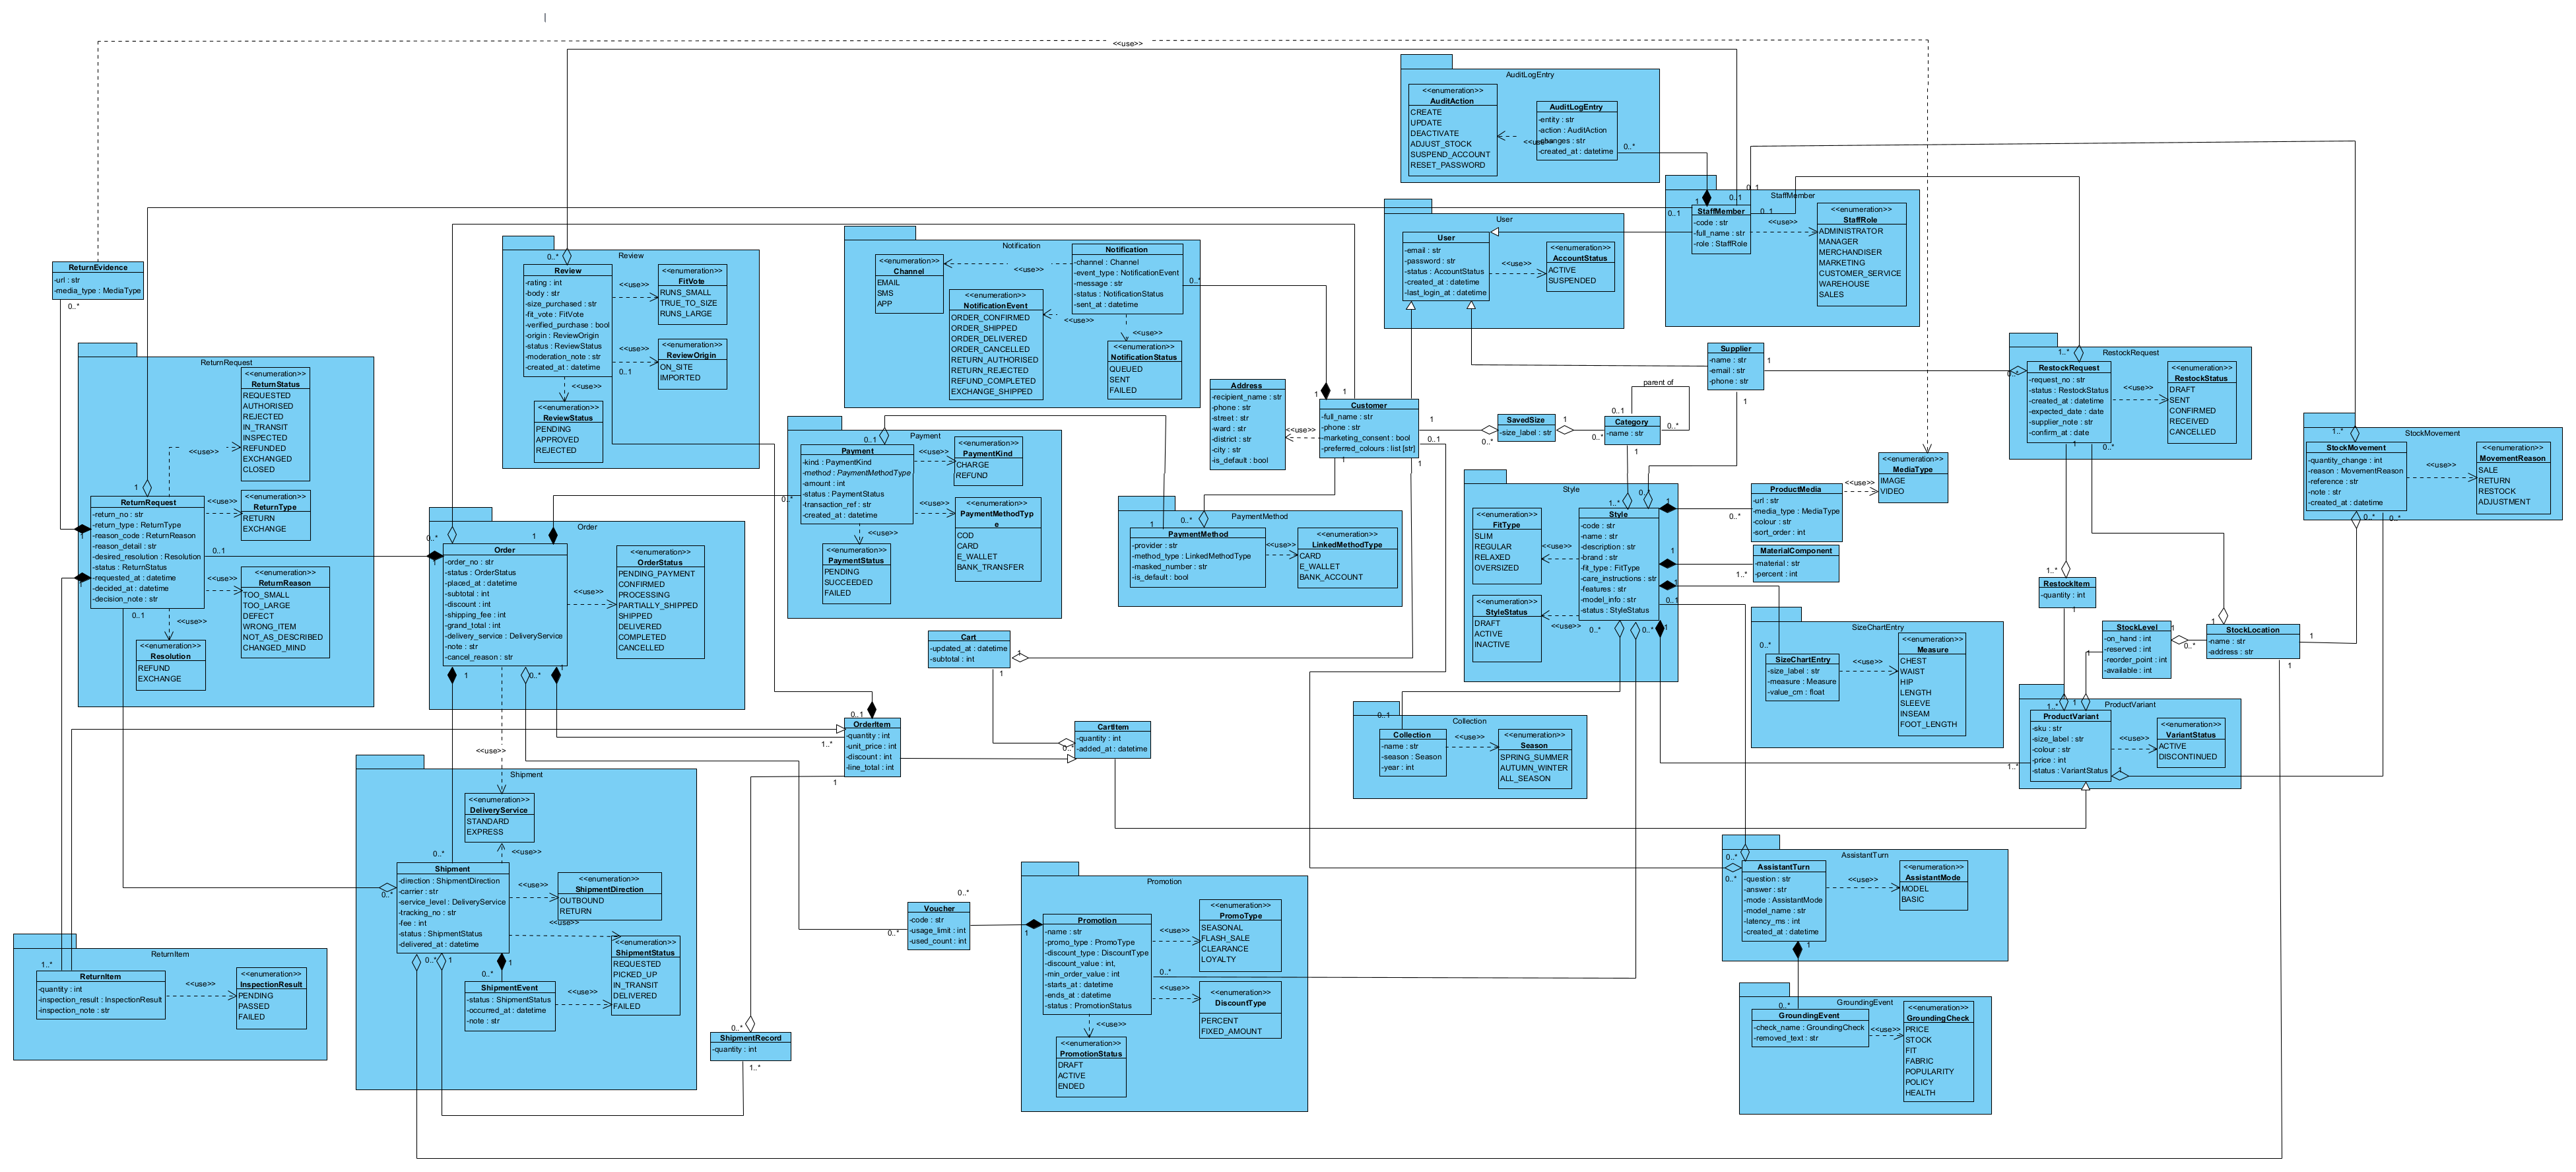
\includegraphics[width=\linewidth,height=0.92\textheight,keepaspectratio]{an_full.png}
\caption{Analysis class diagram of the ABC Fashion E-Commerce Information System (Visual Paradigm)}
\label{fig:analysisfull}
\end{figure}
\end{landscape}

\begin{figure}[H]
\centering
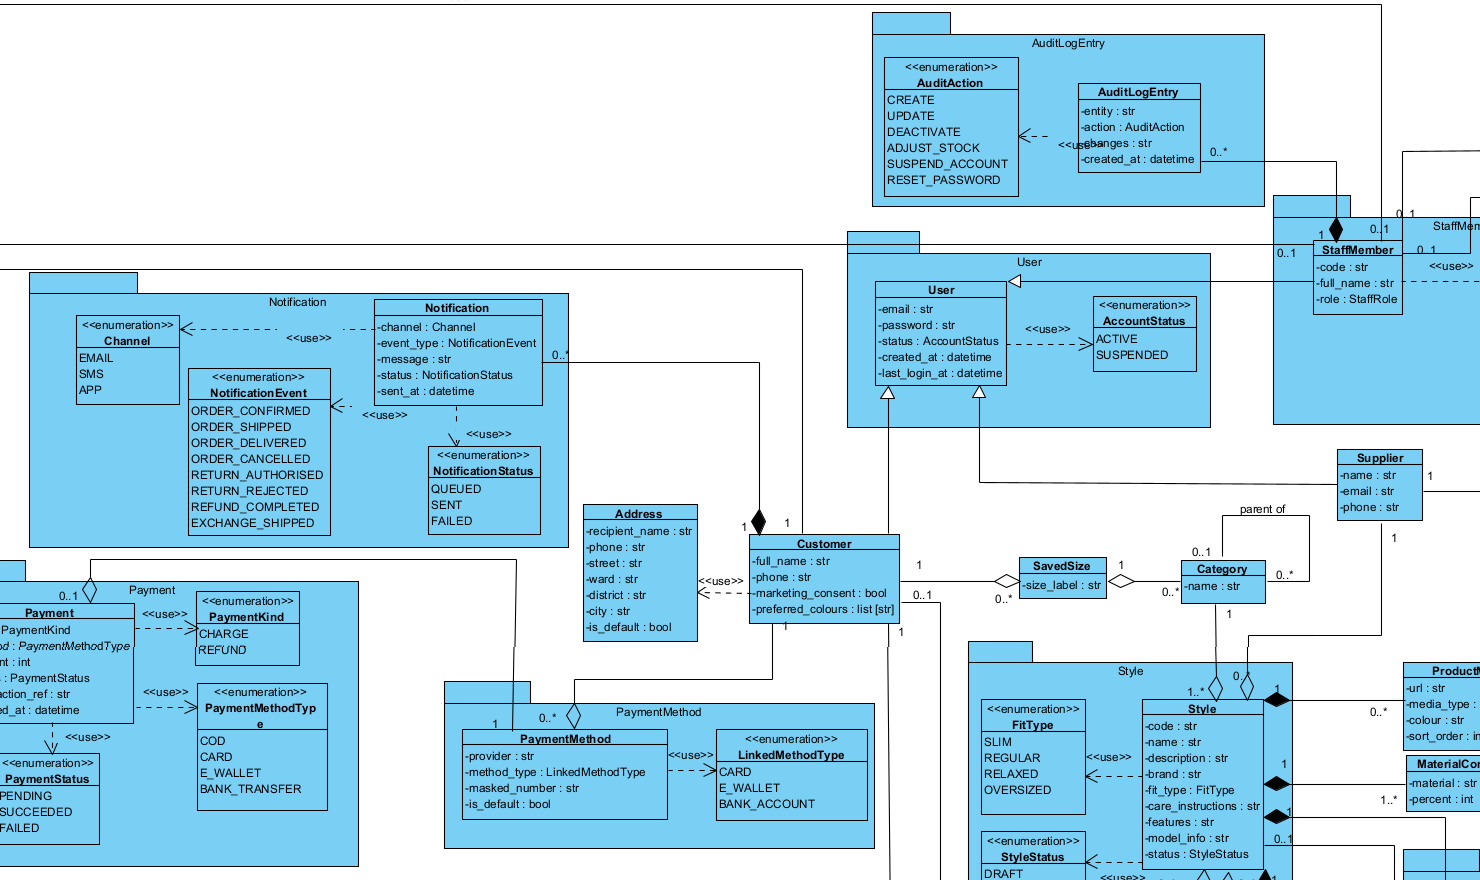
\includegraphics[width=\textwidth,height=0.80\textheight,keepaspectratio]{an_p1_accounts.png}
\caption{Analysis class diagram, part 1 --- users, customers, staff, suppliers, notifications and audit log}
\label{fig:an1}
\end{figure}

\begin{figure}[H]
\centering
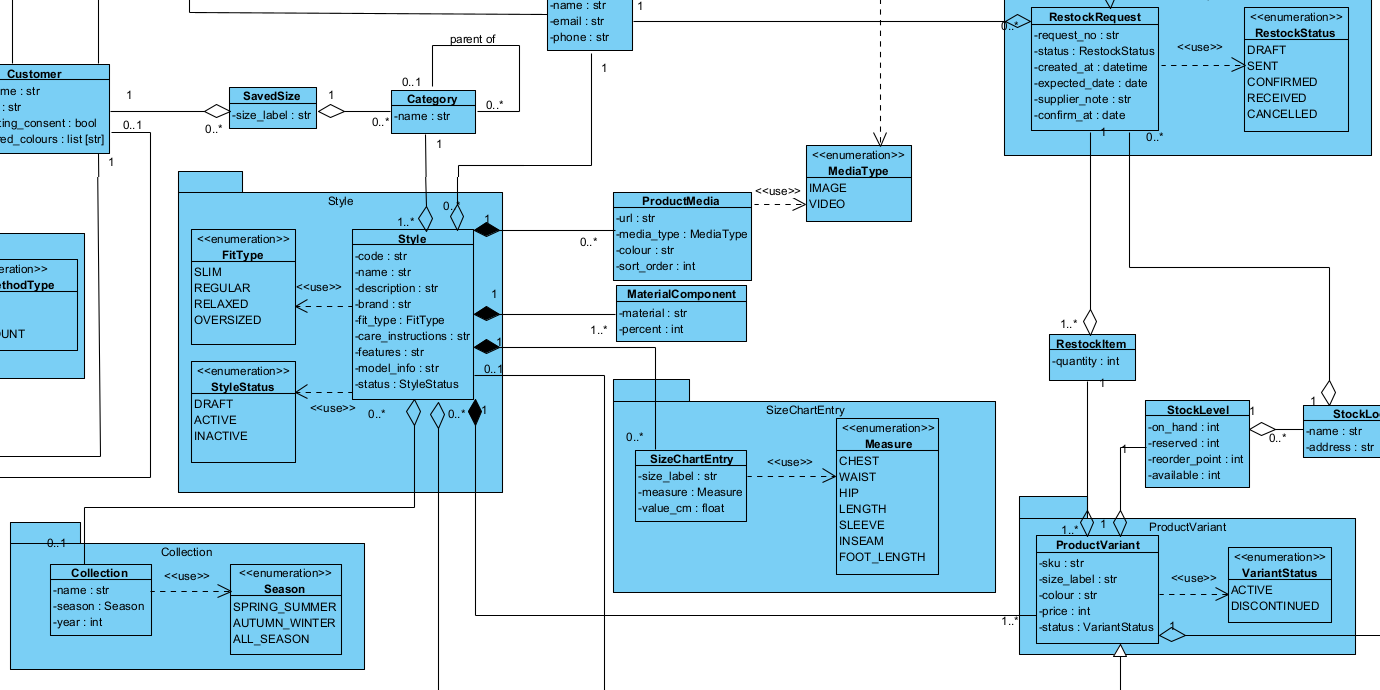
\includegraphics[width=\textwidth,height=0.80\textheight,keepaspectratio]{an_p2_catalogue.png}
\caption{Analysis class diagram, part 2 --- catalogue: category, style, collection and variants}
\label{fig:an2}
\end{figure}

\begin{figure}[H]
\centering
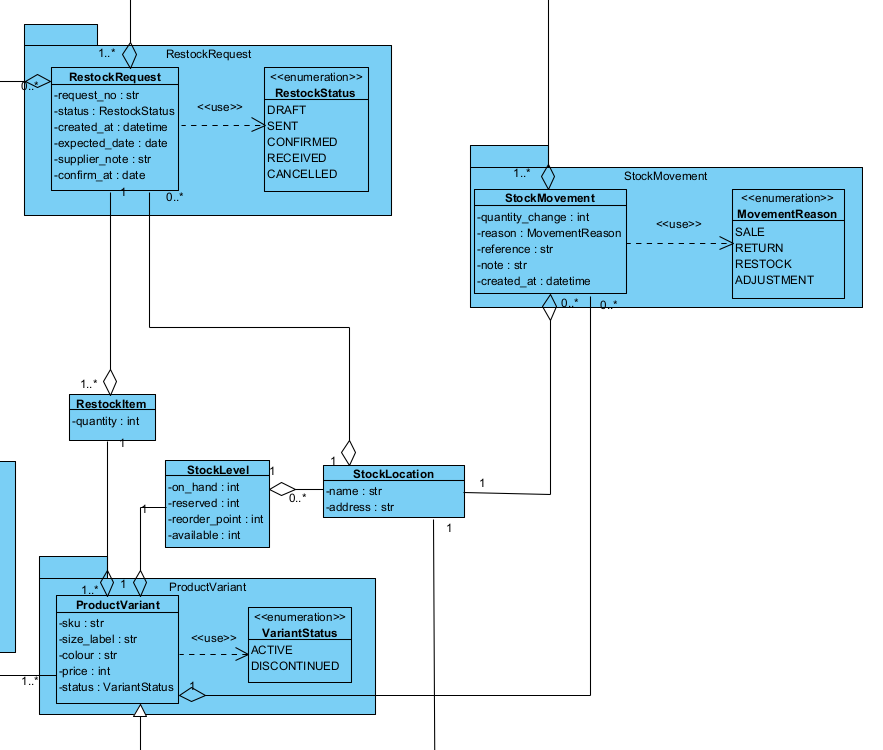
\includegraphics[width=0.85\textwidth,height=0.80\textheight,keepaspectratio]{an_p3_inventory.png}
\caption{Analysis class diagram, part 3 --- inventory and restocking}
\label{fig:an3}
\end{figure}

\begin{figure}[H]
\centering
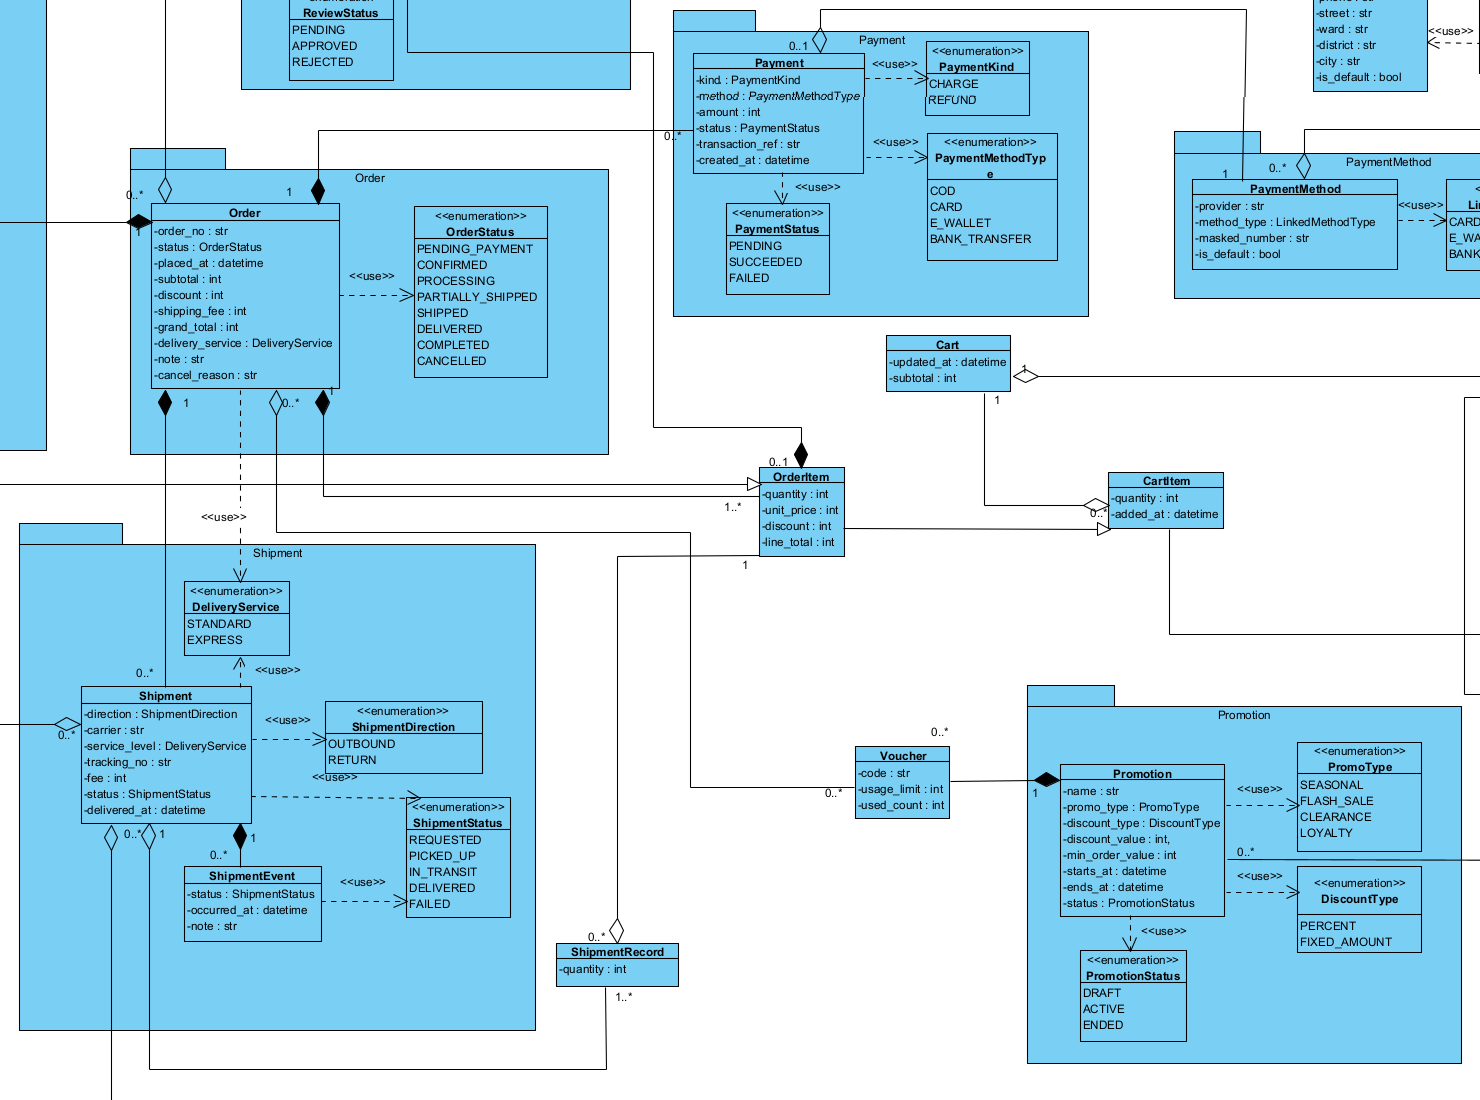
\includegraphics[width=\textwidth,height=0.80\textheight,keepaspectratio]{an_p4_orders.png}
\caption{Analysis class diagram, part 4 --- cart, order, payment, shipment and promotion}
\label{fig:an4}
\end{figure}

\begin{figure}[H]
\centering
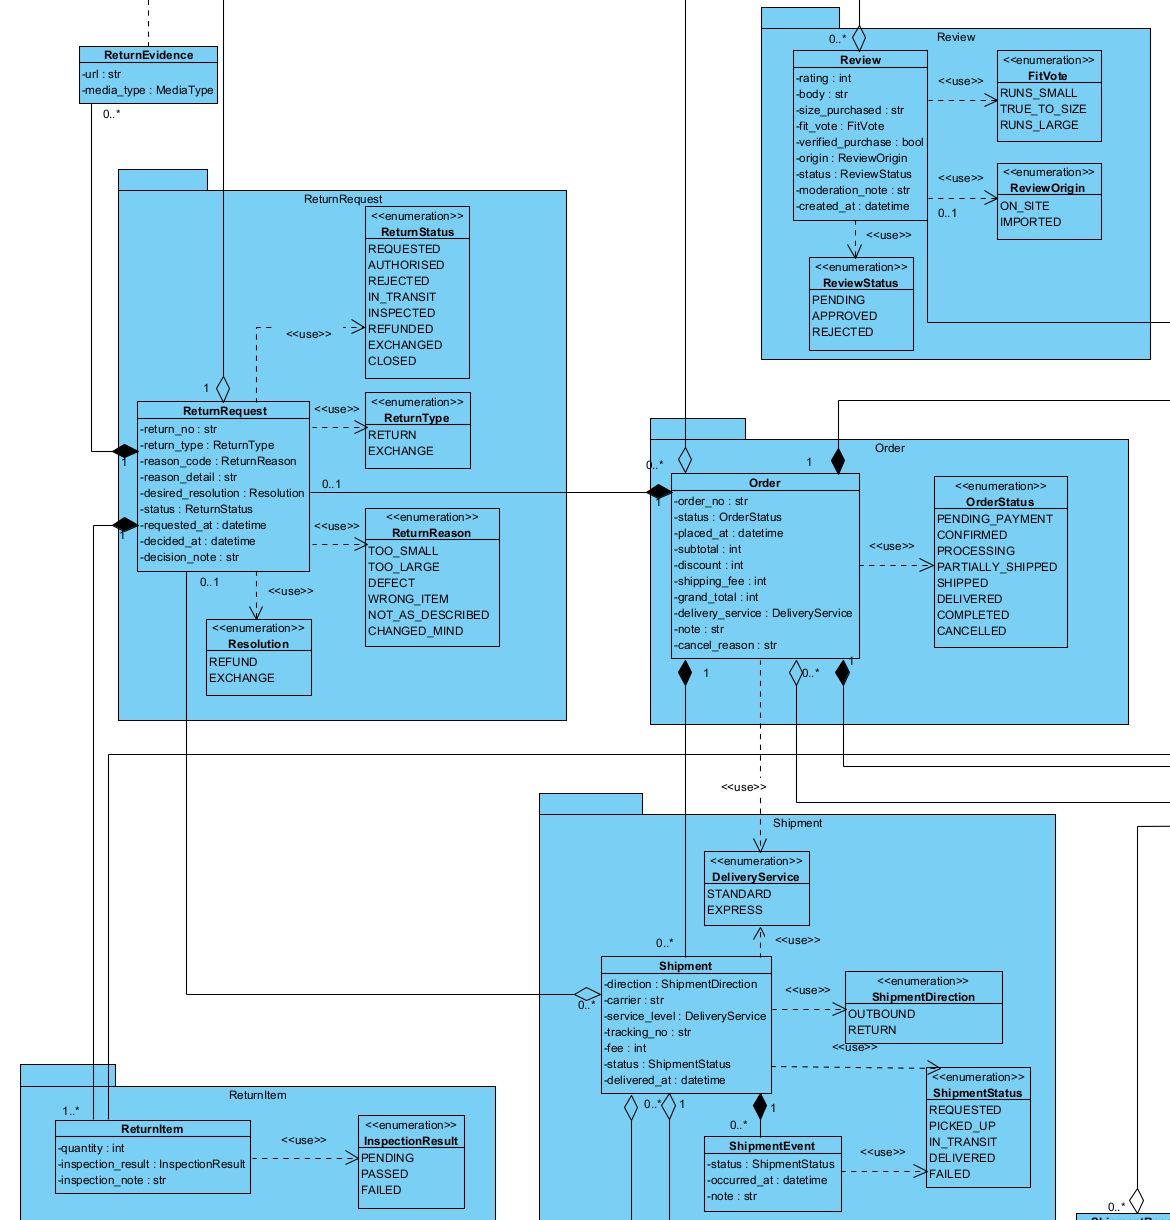
\includegraphics[width=\textwidth,height=0.80\textheight,keepaspectratio]{an_p5_returns_reviews.png}
\caption{Analysis class diagram, part 5 --- returns, exchanges and reviews}
\label{fig:an5}
\end{figure}

\begin{figure}[H]
\centering
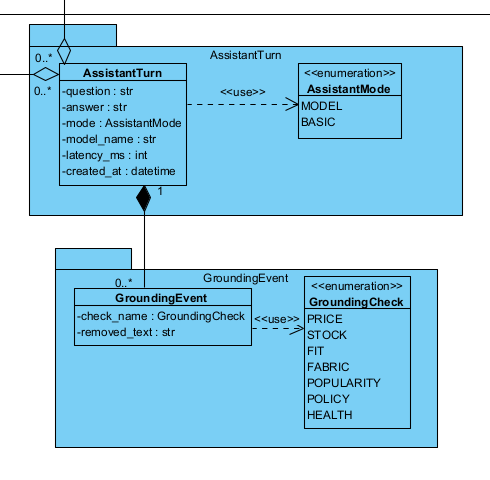
\includegraphics[width=0.6\textwidth,height=0.50\textheight,keepaspectratio]{an_p6_assistant.png}
\caption{Analysis class diagram, part 6 --- AI assistant log}
\label{fig:an6}
\end{figure}

\subsection{Description of the Classes}
\label{subsec:classwords}
Table~\ref{tab:classes} describes every class, its attributes with their Python types and the requirement it comes from. Money is stored as \texttt{int} because Vietnamese dong has no minor unit. Constraints that a Python type cannot express (maximum length, ranges, uniqueness) are listed in the last column and are enforced in the data model.

{\small
\begin{xltabular}{\textwidth}{@{}L{3.0cm} L{4.8cm} Y@{}}
\caption{Analysis classes, attributes and meaning}\label{tab:classes}\\
\toprule
\textbf{Class} & \textbf{Attributes} & \textbf{Meaning, rules and source} \\ \midrule
\endfirsthead
\toprule
\textbf{Class} & \textbf{Attributes} & \textbf{Meaning, rules and source} \\ \midrule
\endhead
\bottomrule
\endlastfoot
\multicolumn{3}{@{}l}{\emph{Users and administration (Figure~\ref{fig:an1})}} \\
\textsf{User} (abstract) & email: str; password: str; status: AccountStatus; created\_at: datetime; last\_login\_at: datetime & Anyone who can log in. The e-mail is unique and is the login name; the password is stored only as a hash; a suspended account cannot log in (FR01, FR02, FR37). Never instantiated on its own \\
\textsf{Customer} & full\_name: str; phone: str; marketing\_consent: bool; preferred\_colours: list[str] & A shopper; one record per person (P6). \texttt{marketing\_consent} records whether the customer agreed to receive promotional e-mail and SMS (FR03) \\
\textsf{StaffMember} & code: str; full\_name: str; role: StaffRole & An employee with a unique staff code; the role decides which use cases are allowed (FR02) \\
\textsf{Supplier} & name: str; email: str; phone: str & A brand or manufacturer. It inherits the login e-mail from \textsf{User}; its own \texttt{email} is the company contact address that receives restock requests (FR24, UC17) \\
\textsf{Address} & recipient\_name, phone, street, ward, district, city: str; is\_default: bool & A delivery address in the address book of a customer; exactly one is the default (FR03) \\
\textsf{PaymentMethod} & provider: str; method\_type: LinkedMethodType; masked\_number: str; is\_default: bool & A card, e-wallet or bank account linked through the Payment Service; only the last four digits are kept (NFR04, UC03) \\
\textsf{SavedSize} & size\_label: str & The size a customer wears in one category, used to preselect sizes and recommend styles (FR03, FR09) \\
\textsf{Notification} & channel: Channel; event\_type: NotificationEvent; message: str; status: NotificationStatus; sent\_at: datetime & A message sent to a customer about an order or a return (FR30) \\
\textsf{AuditLogEntry} & entity: str; action: AuditAction; changes: str; created\_at: datetime & A change made by a staff member to catalogue, stock or accounts, with old and new values (FR37, FR38) \\ \addlinespace
\multicolumn{3}{@{}l}{\emph{Catalogue (Figure~\ref{fig:an2})}} \\
\textsf{Category} & name: str & A browsing category (tops, bottoms, shoes\ldots); categories form a tree (FR06) \\
\textsf{Collection} & name: str; season: Season; year: int & A seasonal collection (FR04) \\
\textsf{Style} & code, name, description, brand: str; fit\_type: FitType; care\_instructions, features, model\_info: str; status: StyleStatus & The product as customers see it (a design such as ``Linen Slim Shirt''), identified by its style code. A style is published only when composition, size chart and care instructions are complete (objective O2); its texts are the catalogue facts used by the AI assistant (FR40) \\
\textsf{MaterialComponent} & material: str; percent: int & One line of the composition (``95\% cotton''); the percentages of a style add up to 100 \\
\textsf{SizeChartEntry} & size\_label: str; measure: Measure; value\_cm: float & One cell of the size chart (size M, chest, 96.0 cm) (FR05) \\
\textsf{ProductVariant} & sku: str; size\_label: str; colour: str; price: int; status: VariantStatus & The SKU: one size and colour of a style with its own price. It is the unit that is sold, stocked and restocked (FR05, FR08, P1). The SKU is unique \\
\textsf{ProductMedia} & url: str; media\_type: MediaType; colour: str; sort\_order: int & An image or video of a style, optionally for one colour (FR05) \\ \addlinespace
\multicolumn{3}{@{}l}{\emph{Inventory and restocking (Figure~\ref{fig:an3})}} \\
\textsf{StockLocation} & name: str; address: str & A warehouse (Ha Noi, Ho Chi Minh City) \\
\textsf{StockLevel} & on\_hand: int; reserved: int; reorder\_point: int; available: int & The stock record of one variant: units on the shelf, units reserved for orders not yet shipped, the threshold that triggers a restock suggestion, and \texttt{available} = \texttt{on\_hand} $-$ \texttt{reserved}, which customers see (FR08, FR14, FR22, NFR10) \\
\textsf{StockMovement} & quantity\_change: int; reason: MovementReason; reference: str; note: str; created\_at: datetime & One change of \texttt{on\_hand}: negative for a sale or an adjustment out, positive for a return or a restock; \texttt{reference} is the order, return or restock number that caused it. The movements of a variant add up to its stock on hand (FR23, FR38, NFR11) \\
\textsf{RestockRequest} & request\_no: str; status: RestockStatus; created\_at: datetime; expected\_date: date; supplier\_note: str; confirm\_at: date & A reorder sent to a supplier. The supplier logs in, confirms it (\texttt{confirm\_at}) and gives the expected delivery date (FR24, UC17) \\
\textsf{RestockItem} & quantity: int & One line of a restock request: a variant and the quantity ordered; a variant appears at most once in a request \\ \addlinespace
\multicolumn{3}{@{}l}{\emph{Cart, order, payment, shipment and promotion (Figure~\ref{fig:an4})}} \\
\textsf{Cart} & updated\_at: datetime; subtotal: int & The shopping cart of a customer, shared by website and app (FR10--FR12, NFR12) \\
\textsf{CartItem} & quantity: int; added\_at: datetime & A variant put in the cart. As a specialisation of \textsf{ProductVariant} it carries the SKU, size, colour and price of the article (FR10, FR11) \\
\textsf{Order} & order\_no: str; status: OrderStatus; placed\_at: datetime; subtotal, discount, shipping\_fee, grand\_total: int; delivery\_service: DeliveryService; note: str; cancel\_reason: str & A purchase. \texttt{grand\_total} = \texttt{subtotal} $-$ \texttt{discount} + \texttt{shipping\_fee} (UC30); the status follows the order life cycle; \texttt{cancel\_reason} is required when the order is cancelled (FR13--FR18) \\
\textsf{OrderItem} & quantity, unit\_price, discount, line\_total: int & An article of an order. It specialises \textsf{CartItem}: the article chosen in the cart becomes an order item and keeps the price at the time of ordering, its share of the discount and \texttt{line\_total} = \texttt{unit\_price} $\times$ \texttt{quantity} $-$ \texttt{discount} (FR13, FR14) \\
\textsf{Payment} & kind: PaymentKind; method: PaymentMethodType; amount: int; status: PaymentStatus; transaction\_ref: str; created\_at: datetime & One charge or refund through the Payment Service with its transaction reference (FR19, FR20). Refunds of a return are payments of kind \texttt{REFUND} of the same order \\
\textsf{Promotion} & name: str; promo\_type: PromoType; discount\_type: DiscountType; discount\_value: int; min\_order\_value: int; starts\_at, ends\_at: datetime; status: PromotionStatus & A campaign (seasonal, flash sale, clearance, loyalty) with a percentage or fixed discount and a validity period (FR33, UC15) \\
\textsf{Voucher} & code: str; usage\_limit: int; used\_count: int & A discount code of a promotion; \texttt{used\_count} never exceeds \texttt{usage\_limit} (FR21, UC26) \\
\textsf{Shipment} & direction: ShipmentDirection; carrier: str; service\_level: DeliveryService; tracking\_no: str; fee: int; status: ShipmentStatus; delivered\_at: datetime & One parcel handled by the Shipping Provider, either to the customer or back from the customer (FR25, FR26) \\
\textsf{ShipmentRecord} & quantity: int & How many units of an order item travel in a shipment; it makes split shipments possible (FR15, UC28) \\
\textsf{ShipmentEvent} & status: ShipmentStatus; occurred\_at: datetime; note: str & A status update reported by the carrier (FR26, UC11) \\ \addlinespace
\multicolumn{3}{@{}l}{\emph{Returns, reviews and AI assistant (Figures~\ref{fig:an5} and~\ref{fig:an6})}} \\
\textsf{ReturnRequest} & return\_no: str; return\_type: ReturnType; reason\_code: ReturnReason; reason\_detail: str; desired\_resolution: Resolution; status: ReturnStatus; requested\_at, decided\_at: datetime; decision\_note: str & A request to return or exchange articles of a delivered order, with the staff decision (FR27, FR28). The reason codes feed the return report (FR36, K3) \\
\textsf{ReturnItem} & quantity: int; inspection\_result: InspectionResult; inspection\_note: str & An article being returned. It specialises \textsf{OrderItem}, so it is the purchased article itself; only an item that passes inspection goes back to stock (FR28, FR29) \\
\textsf{ReturnEvidence} & url: str; media\_type: MediaType & An image or video attached by the customer (FR27) \\
\textsf{Review} & rating: int; body: str; size\_purchased: str; fit\_vote: FitVote; status: ReviewStatus; moderation\_note: str; created\_at: datetime & A rating (1--5) and text written by a customer about an article that was bought, with the size purchased and the fit vote (FR31, FR43). It is checked automatically and held for staff when suspicious (FR32, FR44) \\
\textsf{AssistantTurn} & question, answer: str; mode: AssistantMode; model\_name: str; latency\_ms: int; created\_at: datetime & One question to the AI assistant and its answer; \texttt{mode} is \texttt{BASIC} when the language model is not available (FR39, FR40, NFR13, NFR14) \\
\textsf{GroundingEvent} & check\_name: GroundingCheck; removed\_text: str & One statement removed from an answer because it is not supported by catalogue or reviews (FR45) \\
\end{xltabular}
}

\textbf{Enumerations.} Every attribute whose values come from a closed set has an enumeration as its type (Table~\ref{tab:enums}). In Python each enumeration is a class \texttt{class OrderStatus(str, Enum)} whose members are written in capitals; in the diagram it is connected to the class that uses it by a dependency \guillemotleft use\guillemotright.

{\small
\begin{xltabular}{\textwidth}{@{}L{3.2cm} Y L{3.4cm}@{}}
\caption{Enumerations of the analysis model}\label{tab:enums}\\
\toprule
\textbf{Enumeration} & \textbf{Values} & \textbf{Used by} \\ \midrule
\endfirsthead
\toprule
\textbf{Enumeration} & \textbf{Values} & \textbf{Used by} \\ \midrule
\endhead
\bottomrule
\endlastfoot
AccountStatus & ACTIVE, SUSPENDED & User.\allowbreak status \\
StaffRole & ADMINISTRATOR, MANAGER, MERCHANDISER, MARKETING, CUSTOMER\_SERVICE, WAREHOUSE, SALES & StaffMember.\allowbreak role \\
LinkedMethodType & CARD, E\_WALLET, BANK\_ACCOUNT & PaymentMethod.\allowbreak method\_type \\
FitType & SLIM, REGULAR, RELAXED, OVERSIZED & Style.\allowbreak fit\_type \\
StyleStatus & DRAFT, ACTIVE, INACTIVE & Style.\allowbreak status \\
Season & SPRING\_SUMMER, AUTUMN\_WINTER, ALL\_SEASON & Collection.\allowbreak season \\
Measure & CHEST, WAIST, HIP, LENGTH, SLEEVE, INSEAM, FOOT\_LENGTH & SizeChartEntry.\allowbreak measure \\
VariantStatus & ACTIVE, DISCONTINUED & ProductVariant.\allowbreak status \\
MediaType & IMAGE, VIDEO & ProductMedia, ReturnEvidence \\
MovementReason & SALE, RETURN, RESTOCK, ADJUSTMENT & StockMovement.\allowbreak reason \\
RestockStatus & DRAFT, SENT, CONFIRMED, RECEIVED, CANCELLED & RestockRequest.\allowbreak status \\
OrderStatus & PENDING\_PAYMENT, CONFIRMED, PROCESSING, PARTIALLY\_SHIPPED, SHIPPED, DELIVERED, COMPLETED, CANCELLED & Order.\allowbreak status \\
DeliveryService & STANDARD, EXPRESS & Order, Shipment \\
PaymentKind & CHARGE, REFUND & Payment.\allowbreak kind \\
PaymentMethodType & COD, CARD, E\_WALLET, BANK\_TRANSFER & Payment.\allowbreak method \\
PaymentStatus & PENDING, SUCCEEDED, FAILED & Payment.\allowbreak status \\
PromoType & SEASONAL, FLASH\_SALE, CLEARANCE, LOYALTY & Promotion.\allowbreak promo\_type \\
DiscountType & PERCENT, FIXED\_AMOUNT & Promotion.\allowbreak discount\_type \\
PromotionStatus & DRAFT, ACTIVE, ENDED & Promotion.\allowbreak status \\
ShipmentDirection & OUTBOUND, RETURN & Shipment.\allowbreak direction \\
ShipmentStatus & REQUESTED, PICKED\_UP, IN\_TRANSIT, DELIVERED, FAILED & Shipment, ShipmentEvent \\
ReturnType & RETURN, EXCHANGE & ReturnRequest.\allowbreak return\_type \\
ReturnReason & TOO\_SMALL, TOO\_LARGE, DEFECT, WRONG\_ITEM, NOT\_AS\_DESCRIBED, CHANGED\_MIND & ReturnRequest.\allowbreak reason\_code \\
Resolution & REFUND, EXCHANGE & ReturnRequest.\allowbreak desired\_resolution \\
ReturnStatus & REQUESTED, AUTHORISED, REJECTED, IN\_TRANSIT, INSPECTED, REFUNDED, EXCHANGED, CLOSED & ReturnRequest.\allowbreak status \\
InspectionResult & PENDING, PASSED, FAILED & ReturnItem.\allowbreak inspection\_result \\
FitVote & RUNS\_SMALL, TRUE\_TO\_SIZE, RUNS\_LARGE & Review.\allowbreak fit\_vote \\
ReviewStatus & PENDING, APPROVED, REJECTED & Review.\allowbreak status \\
Channel & EMAIL, SMS, APP & Notification.\allowbreak channel \\
NotificationEvent & ORDER\_CONFIRMED, ORDER\_SHIPPED, ORDER\_DELIVERED, ORDER\_CANCELLED, RETURN\_AUTHORISED, RETURN\_REJECTED, REFUND\_COMPLETED, EXCHANGE\_SHIPPED & Notification.\allowbreak event\_type \\
NotificationStatus & QUEUED, SENT, FAILED & Notification.\allowbreak status \\
AuditAction & CREATE, UPDATE, DEACTIVATE, ADJUST\_STOCK, SUSPEND\_ACCOUNT, RESET\_PASSWORD & AuditLogEntry.\allowbreak action \\
AssistantMode & MODEL, BASIC & AssistantTurn.\allowbreak mode \\
GroundingCheck & PRICE, STOCK, FIT, FABRIC, POPULARITY, POLICY, HEALTH & GroundingEvent.\allowbreak check\_name \\
\end{xltabular}
}

\subsection{Relationships between the Classes}
\label{subsec:relationships}
The diagram uses five kinds of relationship:
\begin{itemize}
  \item \textbf{Generalisation} (hollow triangle) --- the subclass \emph{is a} kind of the superclass and inherits its attributes and relationships.
  \item \textbf{Composition} (filled diamond) --- the part belongs to exactly one whole and is deleted with it, e.g.\ the items of an order.
  \item \textbf{Aggregation} (hollow diamond) --- a weaker ``consists of'' or ``belongs to'' relationship in which both objects can exist separately, e.g.\ a style and its category.
  \item \textbf{Association} (plain line) --- two objects that refer to each other without ownership, e.g.\ the parent of a category.
  \item \textbf{Dependency \guillemotleft use\guillemotright} (dashed arrow) --- a class uses an enumeration as the type of an attribute, or uses another class without keeping a link to it.
\end{itemize}

\textbf{Generalisations.} There are two hierarchies. (1) \textsf{Customer}, \textsf{StaffMember} and \textsf{Supplier} specialise the abstract class \textsf{User}: they share the login data and the account status, but each keeps its own profile. Making the supplier a user lets it log in and confirm restock requests itself instead of by e-mail (UC17). (2) \textsf{ReturnItem} specialises \textsf{OrderItem}, which specialises \textsf{CartItem}, which specialises \textsf{ProductVariant}. This chain expresses that the system works on \emph{the same article} along the whole customer journey: the variant chosen in the cart becomes an order item when the order is placed and a return item when it is sent back. Each step inherits everything known about the article (SKU, size, colour, price, quantity) and adds only its own facts (time added; price paid and discount; inspection result). For this reason an order item does not need a separate link to its variant, a return item does not need a link to the order line or to the variant wanted in an exchange, and a review reaches the style through the order item it is written for. How this hierarchy is stored in tables is decided in the data model (Section~\ref{sec:datamodel}).

\textbf{Multiplicities.} A multiplicity is read at the far end of the line: ``\textsf{Customer} 1 --- 0..* \textsf{Order}'' means that a customer places zero or more orders and that every order belongs to exactly one customer. Table~\ref{tab:relationships} lists every relationship except the dependencies on enumerations, which are listed in Table~\ref{tab:enums}.

{\small
\begin{xltabular}{\textwidth}{@{}L{4.4cm} L{2.1cm} L{1.7cm} Y@{}}
\caption{Relationships of the analysis class diagram}\label{tab:relationships}\\
\toprule
\textbf{Relationship} & \textbf{Kind} & \textbf{Mult.} & \textbf{Meaning and justification} \\ \midrule
\endfirsthead
\toprule
\textbf{Relationship} & \textbf{Kind} & \textbf{Mult.} & \textbf{Meaning and justification} \\ \midrule
\endhead
\bottomrule
\endlastfoot
\multicolumn{4}{@{}l}{\emph{Users and administration}} \\
Customer, StaffMember, Supplier $\rightarrow$ User & Generalisation & --- & Common login data and status (FR01, FR02, UC17) \\
Customer --- Address & Dependency \guillemotleft use\guillemotright & --- & The customer uses the addresses of the address book when checking out (FR03) \\
Customer --- PaymentMethod & Aggregation & 1 / 0..* & A customer links any number of payment methods (UC03) \\
Customer --- SavedSize & Aggregation & 1 / 0..* & Saved sizes of the customer (FR03) \\
Customer --- Notification & Composition & 1 / 0..* & Messages sent to the customer (FR30) \\
StaffMember --- AuditLogEntry & Composition & 1 / 0..* & Every log entry records who made the change (FR38) \\ \addlinespace
\multicolumn{4}{@{}l}{\emph{Catalogue}} \\
SavedSize --- Category & Aggregation & 1 / 0..* & A saved size is valid for a category (FR09) \\
Category --- Category (parent of) & Association & 0..1 / 0..* & A category may have a parent category (FR06) \\
Category --- Style & Aggregation & 1 / 1..* & Every style is in exactly one category; a category lists its styles (FR06) \\
Supplier --- Style & Aggregation & 1 / 0..* & Every style is supplied by one supplier; ABC Fashion does not manufacture (FR24) \\
Collection --- Style & Aggregation & 0..1 / 0..* & A style may belong to a seasonal collection (FR04) \\
Style --- ProductMedia & Composition & 1 / 0..* & Images and videos of the style (FR05) \\
Style --- MaterialComponent & Composition & 1 / 1..* & A style states at least one material (O2) \\
Style --- SizeChartEntry & Composition & 1 / 0..* & The size chart of the style (FR05) \\
Style --- ProductVariant & Composition & 1 / 1..* & A style is sold as at least one size/colour variant (FR05) \\
Promotion --- Style & Aggregation & 0..* / 0..* & Styles included in a promotion (UC27) \\ \addlinespace
\multicolumn{4}{@{}l}{\emph{Inventory and restocking}} \\
ProductVariant --- StockLevel & Aggregation & 1 / 1 & Every variant has exactly one stock record (FR08, FR22) \\
StockLevel --- StockLocation & Aggregation & 0..* / 1 & The stock record is kept at one warehouse \\
StockMovement --- ProductVariant & Aggregation & 0..* / 1 & The variant whose stock changed (FR23) \\
StockMovement --- StockLocation & Aggregation & 0..* / 1 & The warehouse where it changed \\
StaffMember --- StockMovement & Aggregation & 1 / 1..* & Every change of stock is made by a staff member (FR38) \\
Supplier --- RestockRequest & Aggregation & 1 / 0..* & Requests sent to and confirmed by the supplier (FR24, UC17) \\
StaffMember --- RestockRequest & Aggregation & 1 / 1..* & The warehouse staff member who created the request (UC17) \\
RestockRequest --- StockLocation & Aggregation & 0..* / 1 & The warehouse that receives the goods \\
RestockRequest --- RestockItem & Aggregation & 1 / 1..* & A request has at least one line \\
RestockItem --- ProductVariant & Aggregation & 0..* / 1 & Each line orders one variant, at most once per request (FR24) \\ \addlinespace
\multicolumn{4}{@{}l}{\emph{Cart, order, payment, shipment and promotion}} \\
CartItem $\rightarrow$ ProductVariant, OrderItem $\rightarrow$ CartItem & Generalisation & --- & The same article through cart and order (see above) \\
Customer --- Cart & Aggregation & 1 / 1 & One cart per customer, shared by website and app (NFR12) \\
Cart --- CartItem & Aggregation & 1 / 0..* & The cart may be empty (FR10, FR11) \\
Customer --- Order & Aggregation & 1 / 0..* & Orders placed by the customer (FR13) \\
Order --- OrderItem & Composition & 1 / 1..* & An order has at least one item (FR13) \\
Order --- Payment & Composition & 1 / 0..* & Failed attempts, the charge and refunds of the order (FR20) \\
PaymentMethod --- Payment & Aggregation & 1 / 0..1 & The linked method used for a card or e-wallet payment (UC31) \\
Order --- Voucher & Aggregation & 0..* / 0..* & Vouchers redeemed in the order, up to the usage limit (FR21, UC26) \\
Promotion --- Voucher & Composition & 1 / 0..* & The codes of a promotion (FR33) \\
Order --- Shipment & Composition & 1 / 0..* & The parcels of the order; none before payment (FR25) \\
Shipment --- ShipmentRecord & Aggregation & 1 / 1..* & What a parcel contains (FR15) \\
OrderItem --- ShipmentRecord & Aggregation & 1 / 0..* & An item may travel in several parcels (split shipment, UC28) \\
Shipment --- ShipmentEvent & Composition & 1 / 0..* & Tracking history (FR26) \\
Shipment --- StockLocation & Aggregation & 0..* / 1 & The warehouse a parcel leaves from or returns to \\ \addlinespace
\multicolumn{4}{@{}l}{\emph{Returns, reviews and AI assistant}} \\
ReturnItem $\rightarrow$ OrderItem & Generalisation & --- & The returned article is the purchased one (see above) \\
Order --- ReturnRequest & Composition & 1 / 0..1 & At most one return request per order; all articles to be returned are put in it (FR27) \\
ReturnRequest --- ReturnItem & Composition & 1 / 1..* & At least one article is returned \\
ReturnRequest --- ReturnEvidence & Composition & 1 / 0..* & Images and videos of the problem (FR27) \\
StaffMember --- ReturnRequest & Aggregation & 0..1 / 0..* & The staff member who authorises, inspects and closes the request (FR28) \\
ReturnRequest --- Shipment & Aggregation & 0..1 / 0..* & Pickup parcel and replacement parcel of an exchange (UC18) \\
OrderItem --- Review & Composition & 1 / 0..1 & Only a purchased article can be reviewed, once (FR31, FR43) \\
StaffMember --- Review & Aggregation & 0..1 / 0..* & Manual moderation of held reviews (FR32, FR44) \\
Customer --- AssistantTurn & Aggregation & 0..1 / 0..* & Questions asked by a customer; visitors may also ask (FR39) \\
Style --- AssistantTurn & Aggregation & 0..1 / 0..* & The product asked about (FR39) \\
AssistantTurn --- GroundingEvent & Composition & 1 / 0..* & Statements removed from the answer (FR45) \\
\end{xltabular}
}

\textbf{Consequences for the requirements.} Three decisions of the model change how some requirements are met. First, because each variant has one stock record at one warehouse, an order item is always shipped from the warehouse that holds its variant; an order is split into several shipments when its items are stored in different warehouses (FR15). Second, a customer can return or exchange the articles of an order only once, in a single request with several items. Third, every review belongs to a purchased order item, so all reviews are verified purchases and reviews from outside sources are not imported.

% =====================================================================
\section{Data Model}
\label{sec:datamodel}

The data model is the logical and physical design of the database: the relational tables that store the objects of the analysis class diagram, the keys that connect them and the constraints that protect the data. It was drawn as an entity--relationship diagram (ERD) in Visual Paradigm, starting from the analysis class diagram of Section~\ref{sec:analysisclass}, and was then generated as a PostgreSQL~18 database with the administration tool pgAdmin~4. PostgreSQL is an open-source relational DBMS with transactions, row locks and check constraints, which the use cases need (NFR07, NFR10, NFR11).

\subsection{From Classes to Tables}
\label{subsec:mapping}
Every analysis class becomes one table, and the relationships of the class diagram become foreign keys. Table~\ref{tab:mappingrules} lists the rules that were applied and Table~\ref{tab:typemapping} the data types.

{\small
\begin{xltabular}{\textwidth}{@{}L{3.3cm} Y L{4.2cm}@{}}
\caption{Rules for mapping the analysis class diagram to tables}\label{tab:mappingrules}\\
\toprule
\textbf{Model element} & \textbf{Rule applied} & \textbf{Example} \\ \midrule
\endfirsthead
\toprule
\textbf{Model element} & \textbf{Rule applied} & \textbf{Example} \\ \midrule
\endhead
\bottomrule
\endlastfoot
Class & One table named \texttt{tbl} + class name, with a surrogate primary key \texttt{id} generated by the database (identity column) & \textsf{Style} $\rightarrow$ \texttt{tblStyle(id, \ldots)} \\
Attribute & One column with the same \texttt{snake\_case} name & \texttt{tblStyle.\allowbreak care\_instructions} \\
Business identifier & Kept as an ordinary column with a UNIQUE constraint & \texttt{tblProductVariant.\allowbreak sku}, \texttt{tblOrder.\allowbreak order\_no} \\
One-to-many association, aggregation & Foreign key column named after the referenced class + \texttt{Id} in the table on the ``many'' side; NOT NULL when the multiplicity on the ``one'' side is 1, NULL allowed when it is 0..1 & \texttt{tblOrder.\allowbreak customerId}; \texttt{tblStyle.\allowbreak collectionId} (NULL allowed) \\
Composition & As one-to-many, with \texttt{ON DELETE CASCADE}: the parts are deleted with the whole & \texttt{tblCartItem.\allowbreak cartId}, \texttt{tblShipmentEvent.\allowbreak shipmentId} \\
One-to-one association & Foreign key with a UNIQUE constraint & \texttt{tblCart.\allowbreak customerId}, \texttt{tblStockLevel.\allowbreak productVariantId} \\
Many-to-many association & Junction table with two foreign keys and a UNIQUE constraint on the pair & \texttt{tblOrderVoucher}, \texttt{tblPromotionStyle} \\
Self-association & Foreign key to the same table & \texttt{tblCategory.\allowbreak parentId} \\
Generalisation \textsf{User} $\leftarrow$ \textsf{Customer}, \textsf{StaffMember}, \textsf{Supplier} & One table for the superclass and one per subclass; the subclass table keeps its own key and a UNIQUE foreign key to the superclass row (1:1) & \texttt{tblCustomer.\allowbreak userId} $\rightarrow$ \texttt{tblUser} \\
Generalisation chain \textsf{ProductVariant} $\leftarrow$ \textsf{CartItem} $\leftarrow$ \textsf{OrderItem} $\leftarrow$ \textsf{ReturnItem} & Each class has its own table; the inherited data are not copied but reached through a foreign key to the table of the superclass object & \texttt{tblCartItem.\allowbreak productVariantId}, \texttt{tblOrderItem.\allowbreak productVariantId}, \texttt{tblReturnItem.\allowbreak orderItemId} \\
Enumeration & \texttt{varchar(50)} column with a CHECK constraint listing the lowercase values of the Python enumeration & \texttt{tblOrder.\allowbreak status IN ('pending\_payment', \ldots)} \\
Multi-valued attribute & \texttt{list[str]} stored as one comma-separated text, because it is only displayed and never searched & \texttt{tblCustomer.\allowbreak preferred\_colours} \\
Value copied at a point in time & Stored in the referencing table, so that later changes do not rewrite history & \texttt{tblOrderItem.\allowbreak unit\_price} \\
Money & Integer number of Vietnamese dong, so there are no rounding errors & \texttt{price}, \texttt{grand\_total} \\
\end{xltabular}
}

The generalisation chain needs a comment. In the analysis model an order item \emph{is} the cart item and the product variant it came from, so that the system works on the same article from the cart to the return (Section~\ref{subsec:relationships}). A relational table cannot inherit columns, so the chain is stored as a series of references: \texttt{tblCartItem} and \texttt{tblOrderItem} point to the variant, and \texttt{tblReturnItem} points to the order item. Following the references gives the inherited attributes (SKU, size, colour, price paid) without repeating them; only the values that must be frozen at the time of purchase (\texttt{unit\_price}, \texttt{discount}) are stored again in \texttt{tblOrderItem}.

{\small
\begin{xltabular}{\textwidth}{@{}L{3.4cm} L{3.4cm} L{3.2cm} Y@{}}
\caption{Data types: from the Python types of the analysis model to the ERD and PostgreSQL}\label{tab:typemapping}\\
\toprule
\textbf{Python type} & \textbf{ERD (Visual Paradigm)} & \textbf{PostgreSQL 18} & \textbf{Used for} \\ \midrule
\endfirsthead
\toprule
\textbf{Python type} & \textbf{ERD (Visual Paradigm)} & \textbf{PostgreSQL 18} & \textbf{Used for} \\ \midrule
\endhead
\bottomrule
\endlastfoot
\texttt{int} (key) & \texttt{int(10)}, PK & \texttt{integer} identity & \texttt{id} of every table \\
\texttt{int} & \texttt{int(10)} & \texttt{integer} & Quantities, money, foreign keys \\
\texttt{str} & \texttt{varchar(255)} & \texttt{varchar(255)} & Names, texts, codes, URLs \\
Enumeration & \texttt{varchar(50)} & \texttt{varchar(50)} + CHECK & Status, role, reason, \ldots \\
\texttt{bool} & \texttt{bit(1)} & \texttt{boolean} & \texttt{is\_default}, \texttt{marketing\_consent} \\
\texttt{float} & \texttt{float} & \texttt{real} & \texttt{tblSizeChartEntry.\allowbreak value\_cm} \\
\texttt{date} & \texttt{date} & \texttt{date} & \texttt{expected\_date}, \texttt{confirm\_at} \\
\texttt{datetime} & \texttt{datetime} & \texttt{timestamp} & \texttt{created\_at}, \texttt{placed\_at}, \ldots \\
\end{xltabular}
}

\subsection{The Entity--Relationship Diagram}
\label{subsec:erd}
Figure~\ref{fig:erdfull} shows the complete ERD and Figures~\ref{fig:erd1}--\ref{fig:erd4} repeat it in four parts at a readable size. The diagram uses the crow's-foot notation of Visual Paradigm: the key symbol marks the primary key, the green arrow and italic type a foreign key, and the letter \textbf{N} a column that may be NULL. At the ends of a relationship line a bar means ``one'', a circle ``zero'' and a crow's foot ``many'', so that a bar on the parent side and a circle with a crow's foot on the child side reads ``one to zero or many''.

\begin{landscape}
\begin{figure}[p]
\centering
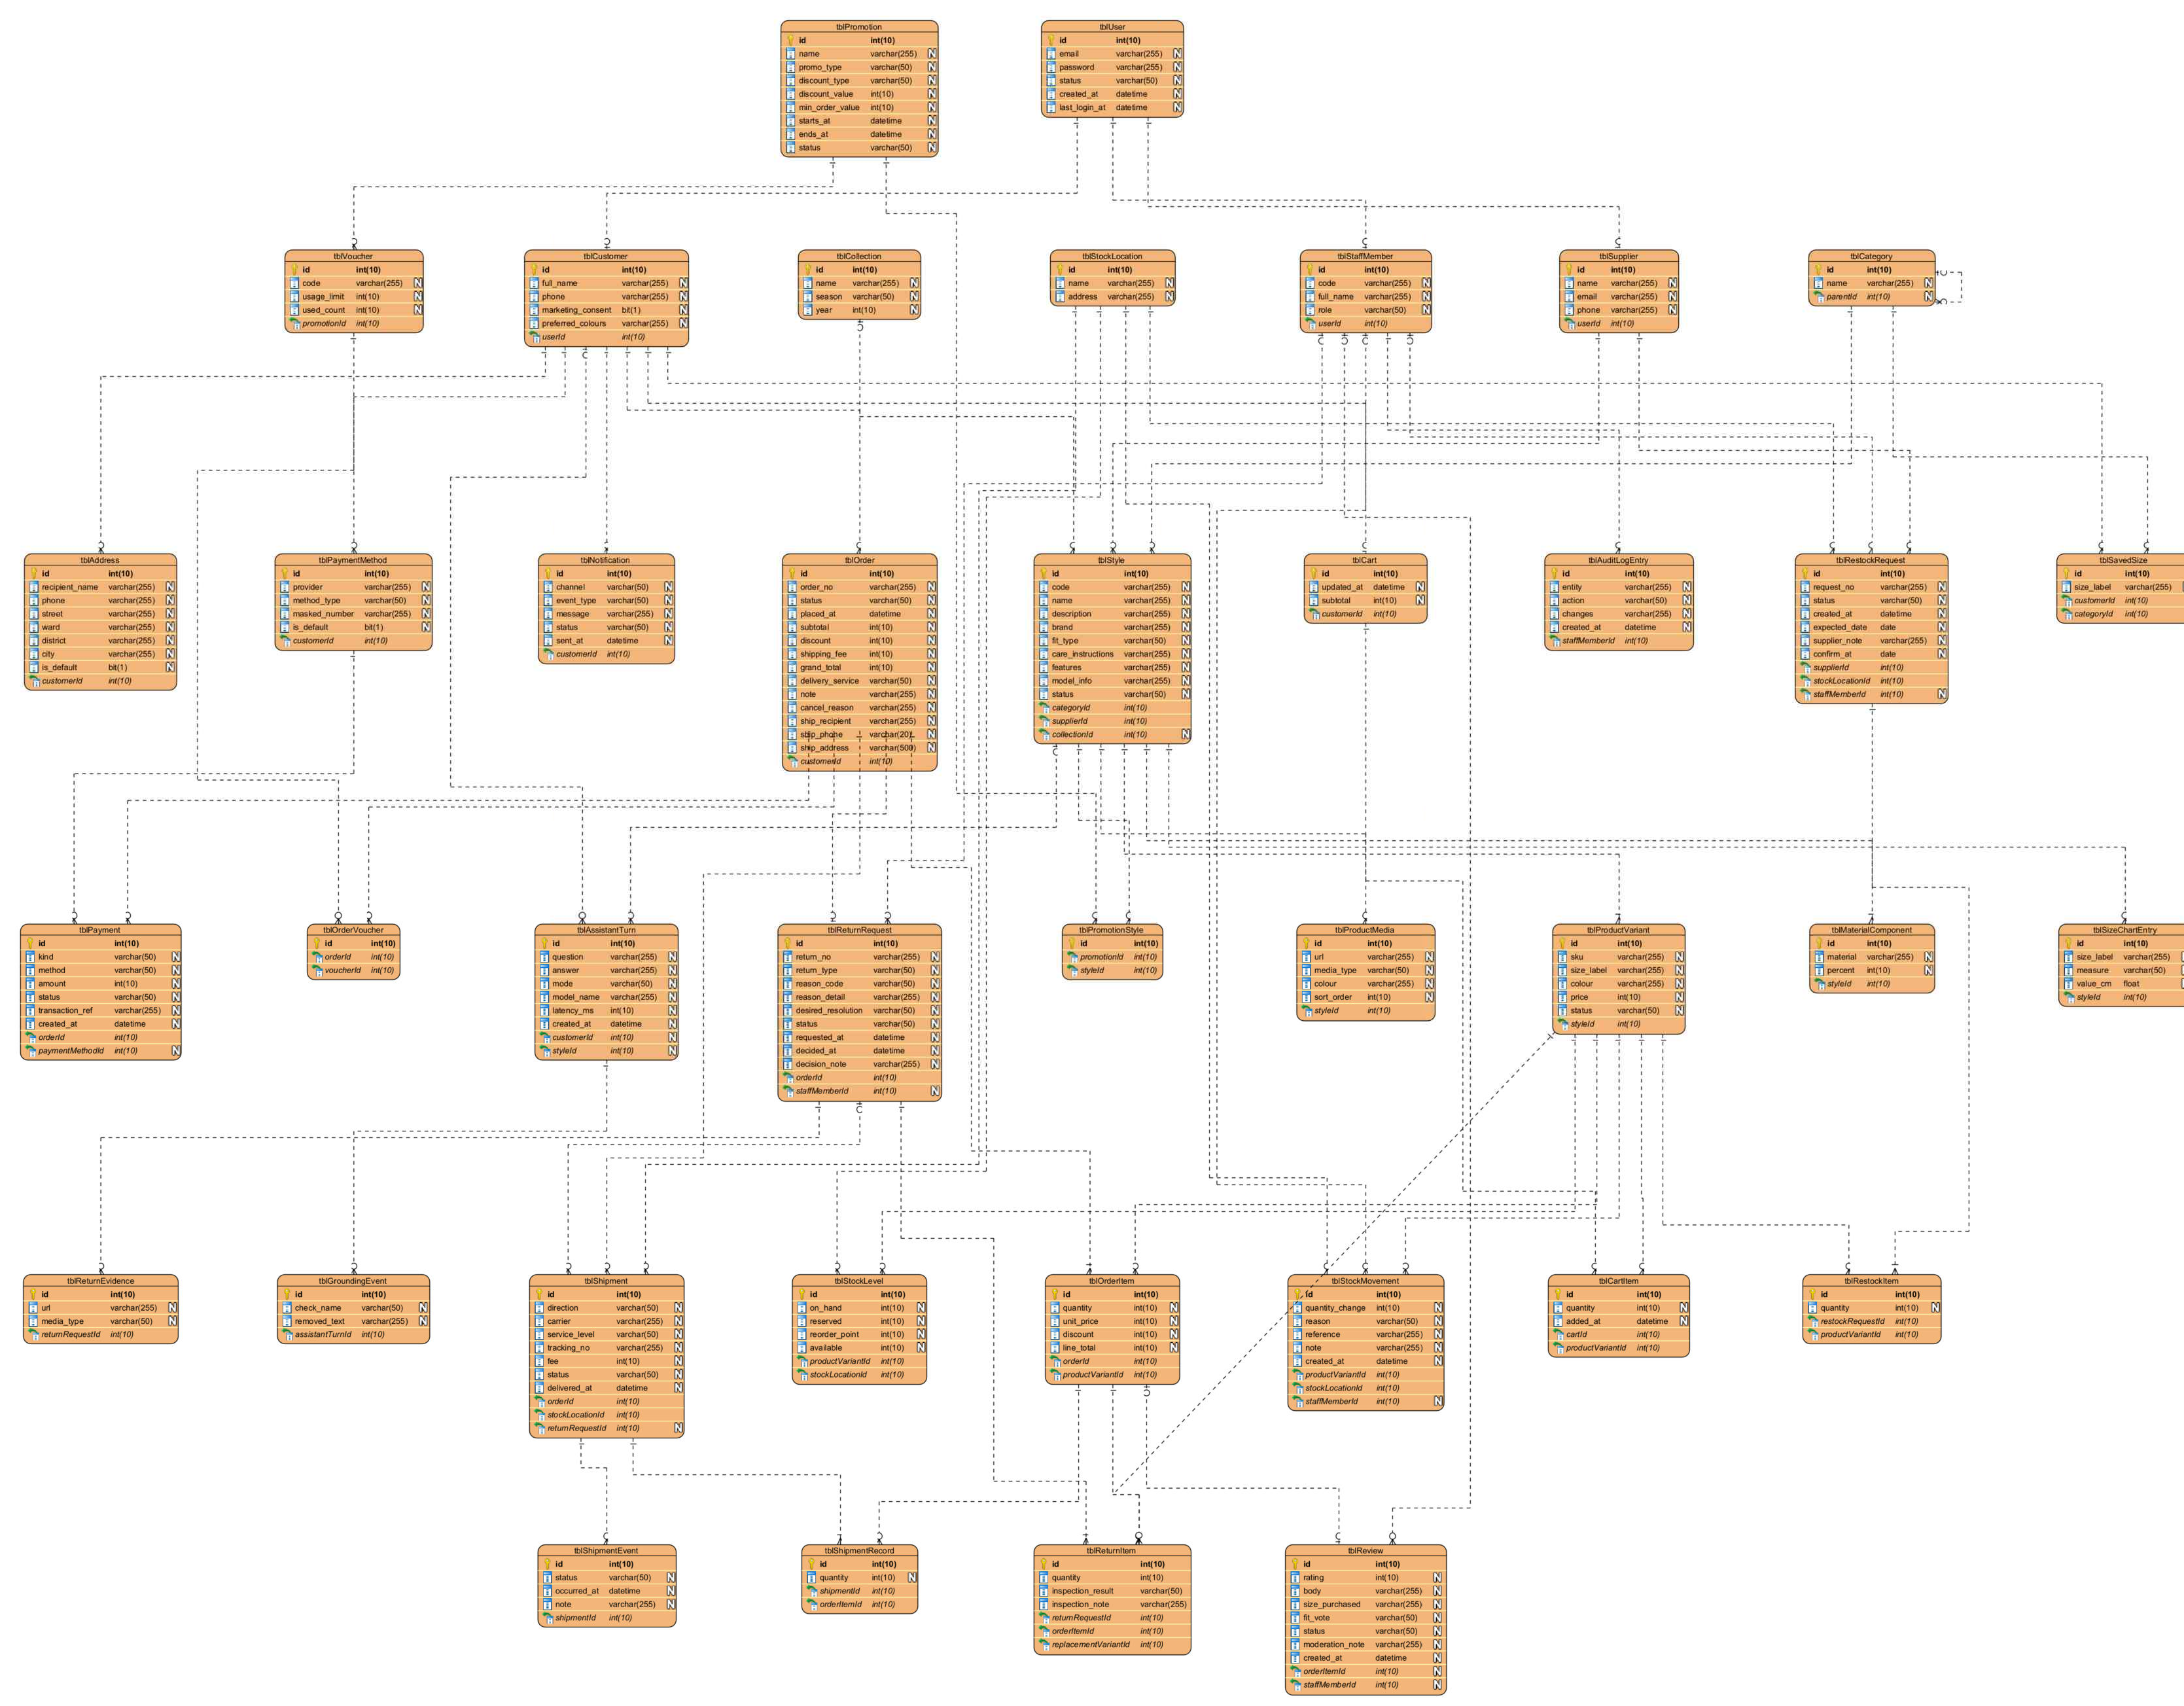
\includegraphics[width=\linewidth,height=0.92\textheight,keepaspectratio]{db_erd.png}
\caption{Entity--relationship diagram of the ABC Fashion database: 39 tables (Visual Paradigm)}
\label{fig:erdfull}
\end{figure}
\end{landscape}

\begin{figure}[H]
\centering
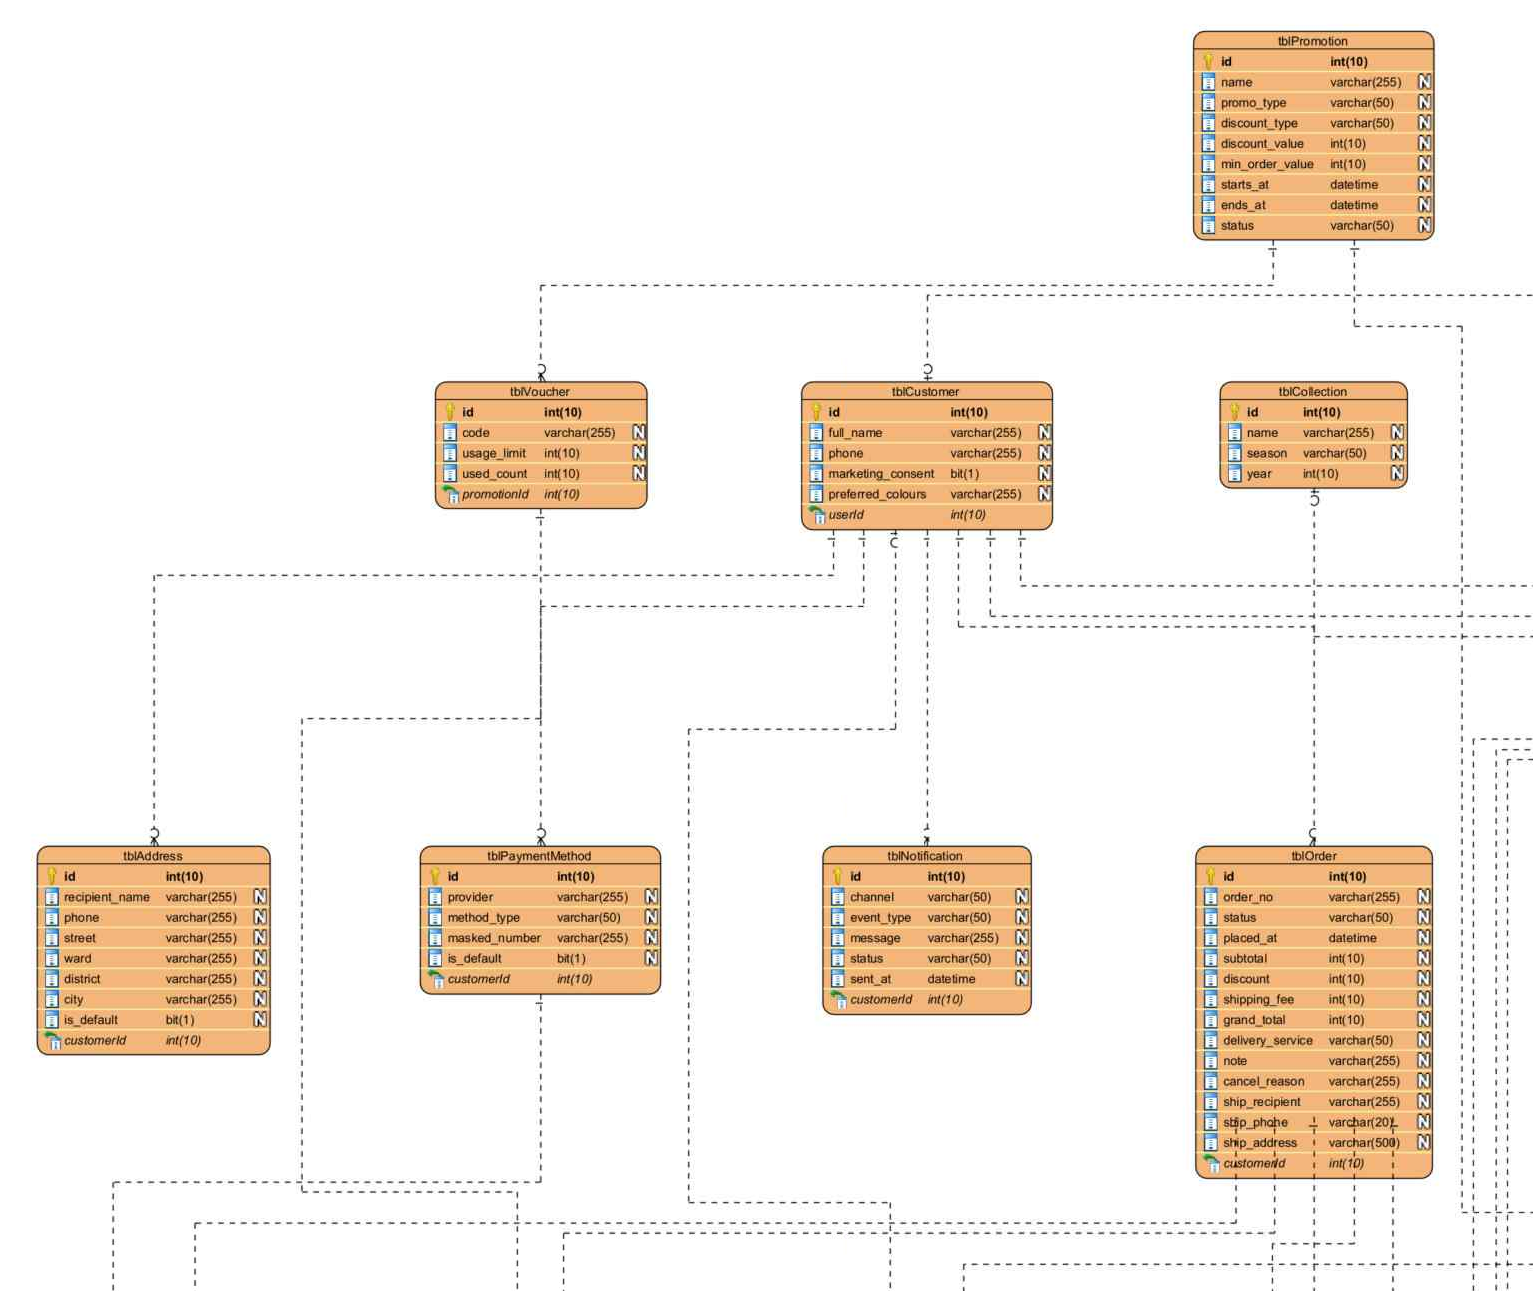
\includegraphics[width=\textwidth,height=0.80\textheight,keepaspectratio]{db_erd_p1.png}
\caption{ERD, part 1 --- promotions, users, customers and their data, orders}
\label{fig:erd1}
\end{figure}

\begin{figure}[H]
\centering
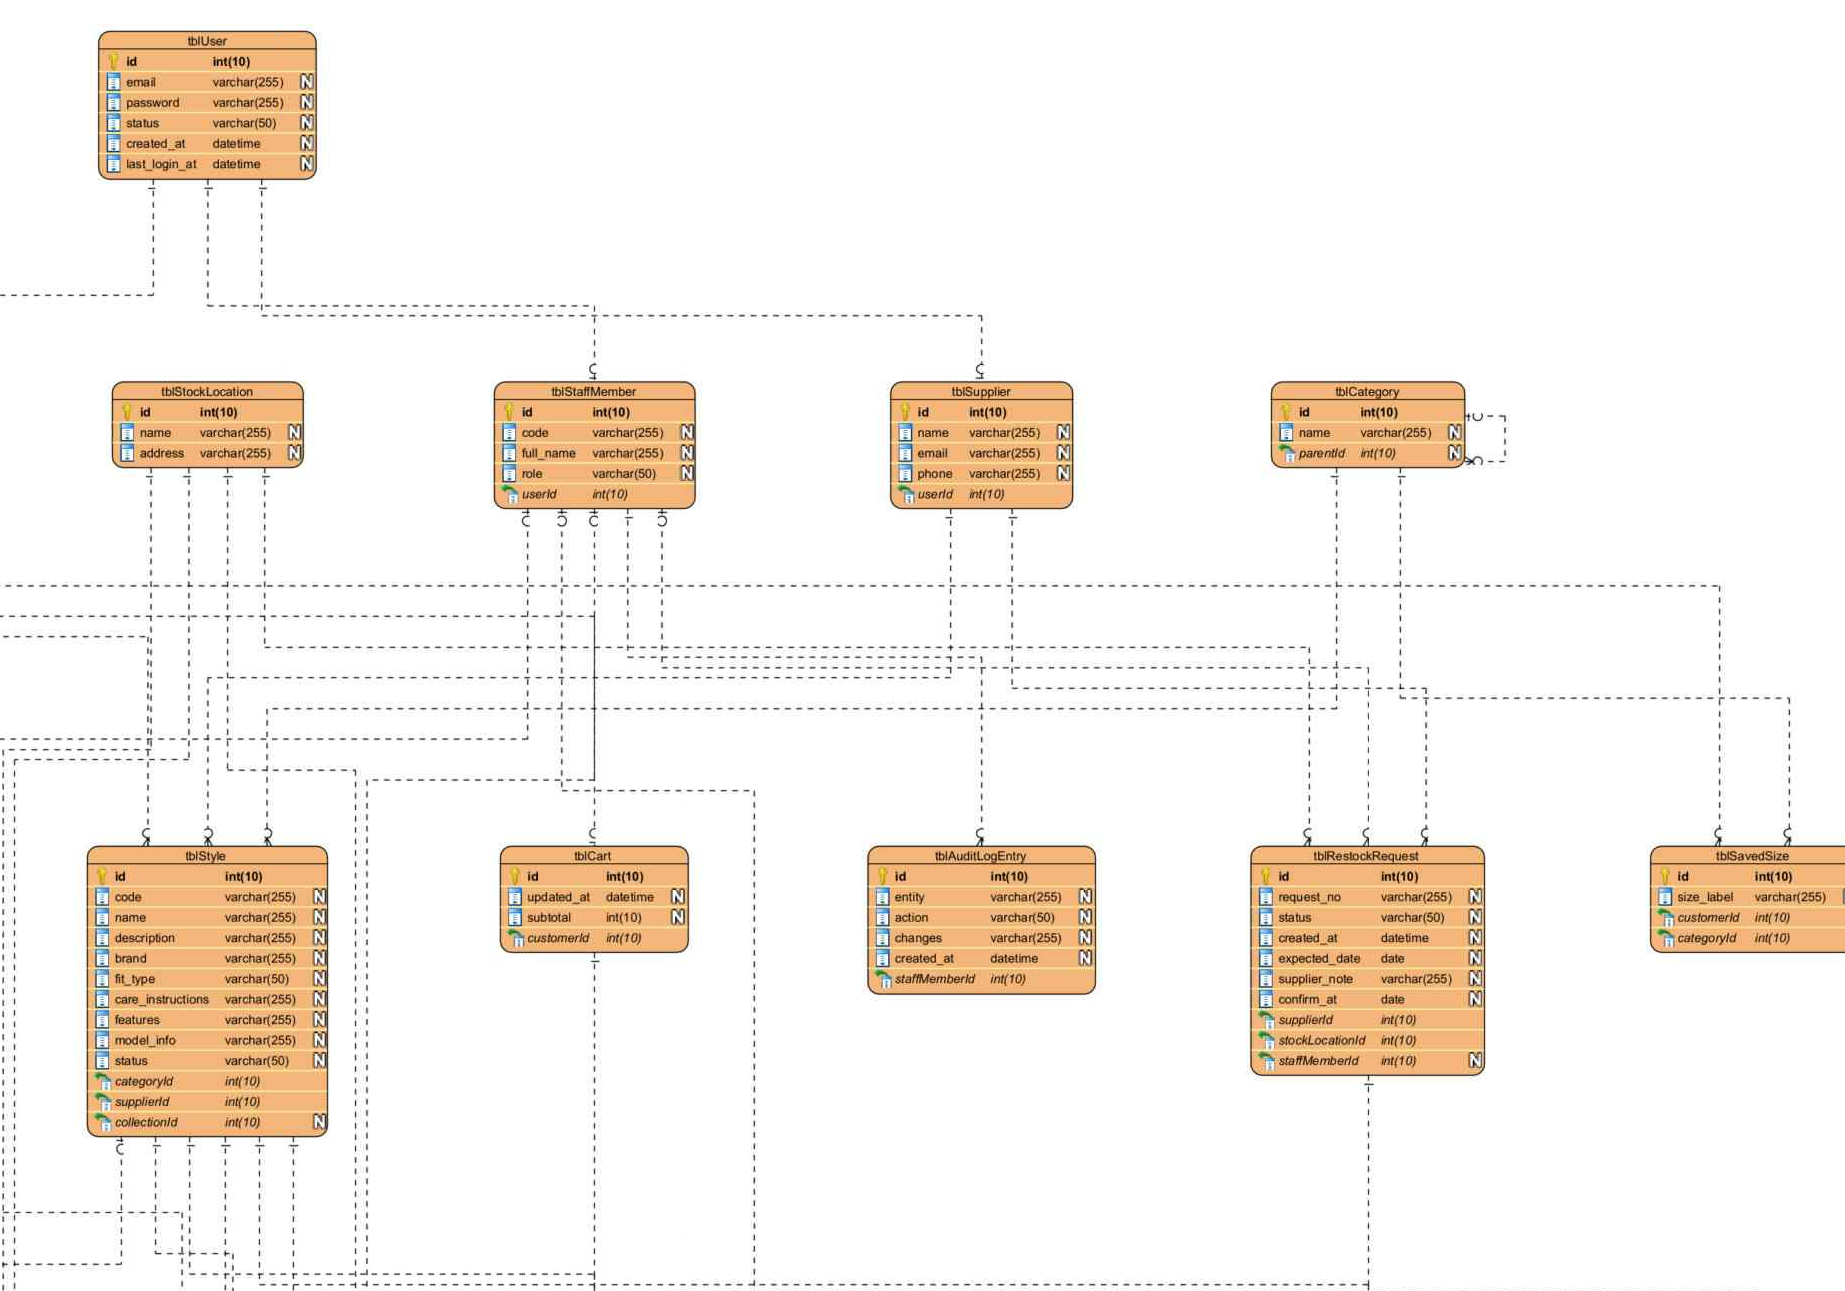
\includegraphics[width=\textwidth,height=0.80\textheight,keepaspectratio]{db_erd_p2.png}
\caption{ERD, part 2 --- catalogue, warehouses, staff, suppliers, cart, audit log and restocking}
\label{fig:erd2}
\end{figure}

\begin{figure}[H]
\centering
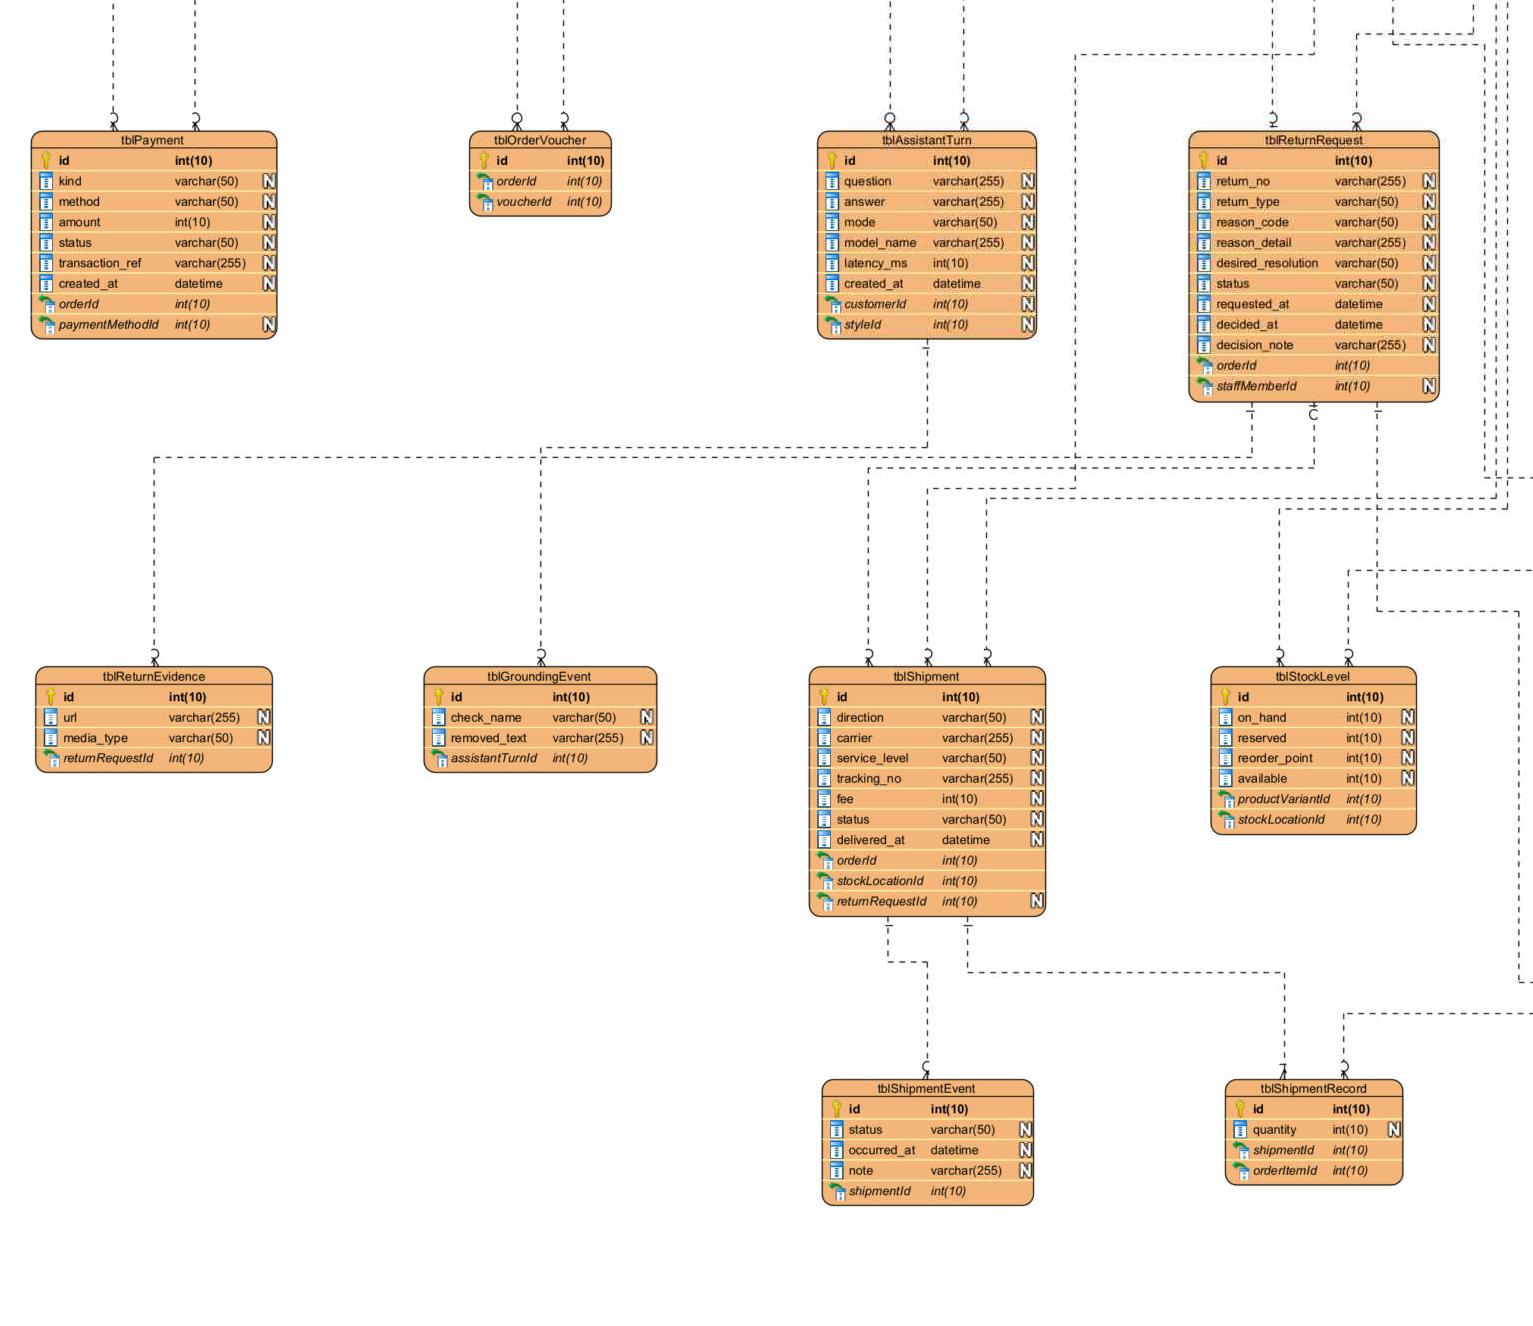
\includegraphics[width=\textwidth,height=0.80\textheight,keepaspectratio]{db_erd_p3.png}
\caption{ERD, part 3 --- payments, vouchers of an order, assistant log, return requests, shipments and stock levels}
\label{fig:erd3}
\end{figure}

\begin{figure}[H]
\centering
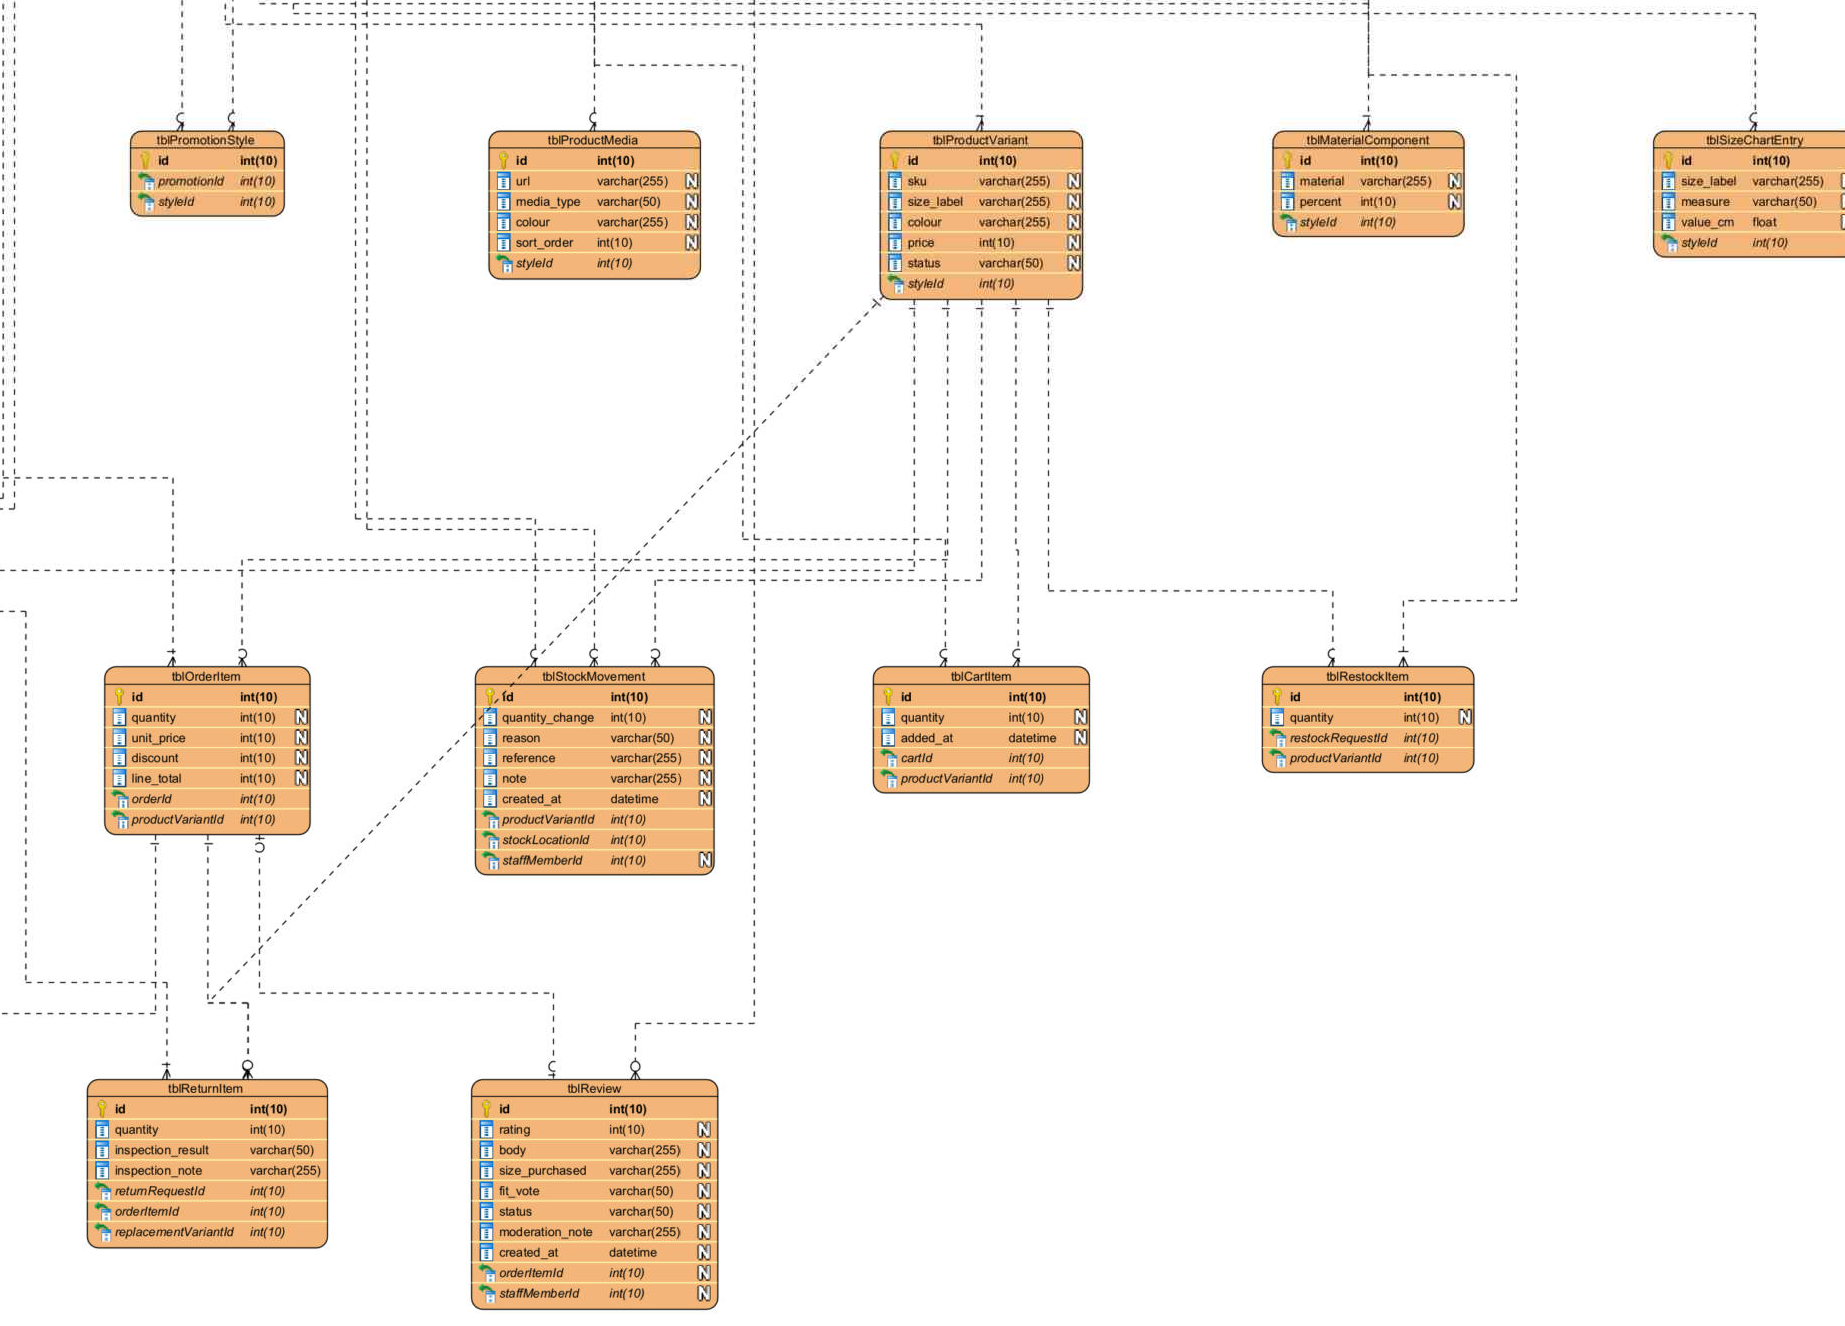
\includegraphics[width=\textwidth,height=0.80\textheight,keepaspectratio]{db_erd_p4.png}
\caption{ERD, part 4 --- variants and their details, order items, cart items, stock movements, restock items, return items and reviews}
\label{fig:erd4}
\end{figure}

\subsection{Tables of the Database}
\label{subsec:tables}
The database contains \textbf{39 tables}: one for each of the 37 analysis classes and the two junction tables \texttt{tblOrderVoucher} and \texttt{tblPromotionStyle}. Together they have 257 columns and \textbf{57 foreign keys}. Table~\ref{tab:tablelist} gives the content of each table.

{\small
\begin{xltabular}{\textwidth}{@{}L{4.4cm} L{3.2cm} Y@{}}
\caption{Tables of the ABC Fashion database}\label{tab:tablelist}\\
\toprule
\textbf{Table} & \textbf{Class} & \textbf{Content} \\ \midrule
\endfirsthead
\toprule
\textbf{Table} & \textbf{Class} & \textbf{Content} \\ \midrule
\endhead
\bottomrule
\endlastfoot
\multicolumn{3}{@{}l}{\emph{Users and administration}} \\
\texttt{tblUser} & User & Login data and status of every account (e-mail unique) \\
\texttt{tblCustomer}, \texttt{tblStaffMember}, \texttt{tblSupplier} & Subclasses of User & Profile of a customer, a staff member (code, role) or a supplier (company contact) \\
\texttt{tblAddress}, \texttt{tblPaymentMethod} & Address, PaymentMethod & Address book; linked payment methods (masked number only) \\
\texttt{tblSavedSize}, \texttt{tblNotification} & SavedSize, Notification & Saved size per category; messages sent to the customer \\
\texttt{tblAuditLogEntry} & AuditLogEntry & Changes made by staff \\ \addlinespace
\multicolumn{3}{@{}l}{\emph{Catalogue}} \\
\texttt{tblCategory}, \texttt{tblCollection} & Category, Collection & Category tree; seasonal collections \\
\texttt{tblStyle} & Style & Product design: name, brand, fit, care, features, model information \\
\texttt{tblMaterialComponent}, \texttt{tblSizeChartEntry}, \texttt{tblProductMedia} & MaterialComponent, SizeChartEntry, ProductMedia & Composition, size chart, images and videos of a style \\
\texttt{tblProductVariant} & ProductVariant & SKU of one size and colour, with its price \\ \addlinespace
\multicolumn{3}{@{}l}{\emph{Inventory and restocking}} \\
\texttt{tblStockLocation}, \texttt{tblStockLevel} & StockLocation, StockLevel & Warehouses; the stock record of each variant \\
\texttt{tblStockMovement} & StockMovement & Ledger of every change of stock \\
\texttt{tblRestockRequest}, \texttt{tblRestockItem} & RestockRequest, RestockItem & Reorders sent to suppliers and their lines \\ \addlinespace
\multicolumn{3}{@{}l}{\emph{Cart, promotion, order and payment}} \\
\texttt{tblCart}, \texttt{tblCartItem} & Cart, CartItem & Shopping cart and its articles \\
\texttt{tblPromotion}, \texttt{tblVoucher}, \texttt{tblPromotionStyle} & Promotion, Voucher, --- & Campaigns, their codes, and the styles of each campaign (junction) \\
\texttt{tblOrder}, \texttt{tblOrderItem}, \texttt{tblOrderVoucher} & Order, OrderItem, --- & Orders with the delivery address copied at the time of ordering (\texttt{ship\_recipient}, \texttt{ship\_phone}, \texttt{ship\_address}), their items, and the vouchers redeemed in each order (junction) \\
\texttt{tblPayment} & Payment & Charges and refunds \\ \addlinespace
\multicolumn{3}{@{}l}{\emph{Shipment, return, review and assistant}} \\
\texttt{tblShipment}, \texttt{tblShipmentRecord}, \texttt{tblShipmentEvent} & Shipment, ShipmentRecord, ShipmentEvent & Parcels, what each parcel contains, tracking events \\
\texttt{tblReturnRequest}, \texttt{tblReturnItem}, \texttt{tblReturnEvidence} & ReturnRequest, ReturnItem, ReturnEvidence & Returns and exchanges, the returned articles, photos and videos \\
\texttt{tblReview} & Review & Rating, text and fit vote of a purchased article; moderation \\
\texttt{tblAssistantTurn}, \texttt{tblGroundingEvent} & AssistantTurn, GroundingEvent & Log of the AI assistant and the statements it removed (Chapter~\ref{ch:ai}) \\
\end{xltabular}
}

\subsection{Relations of the Tables}
\label{subsec:tablerelations}
Every relation of the ERD is implemented by a foreign key. Table~\ref{tab:fkrelations} lists the foreign keys with their cardinality (parent : child), what happens to the child rows when a parent row is deleted, and the meaning of the relation.

{\footnotesize
\begin{xltabular}{\textwidth}{@{}L{4.0cm} L{3.2cm} L{1.3cm} L{1.2cm} Y@{}}
\caption{Foreign keys of the database}\label{tab:fkrelations}\\
\toprule
\textbf{Foreign key} & \textbf{References} & \textbf{Card.} & \textbf{Delete} & \textbf{Meaning} \\ \midrule
\endfirsthead
\toprule
\textbf{Foreign key} & \textbf{References} & \textbf{Card.} & \textbf{Delete} & \textbf{Meaning} \\ \midrule
\endhead
\bottomrule
\endlastfoot
\multicolumn{5}{@{}l}{\emph{Users and administration}} \\
\texttt{tblCustomer}.\allowbreak\texttt{userId} & \texttt{tblUser} & 1 : 0..1 & restrict & Generalisation User--Customer: the login account of the customer \\
\texttt{tblStaffMember}.\allowbreak\texttt{userId} & \texttt{tblUser} & 1 : 0..1 & restrict & Generalisation User--StaffMember \\
\texttt{tblSupplier}.\allowbreak\texttt{userId} & \texttt{tblUser} & 1 : 0..1 & restrict & Generalisation User--Supplier: the supplier logs in to confirm restocks \\
\texttt{tblAddress}.\allowbreak\texttt{customerId} & \texttt{tblCustomer} & 1 : 0..* & cascade & Address book of the customer \\
\texttt{tblPaymentMethod}.\allowbreak\texttt{customerId} & \texttt{tblCustomer} & 1 : 0..* & cascade & Linked cards, e-wallets and bank accounts \\
\texttt{tblNotification}.\allowbreak\texttt{customerId} & \texttt{tblCustomer} & 1 : 0..* & cascade & Messages sent to the customer \\
\texttt{tblSavedSize}.\allowbreak\texttt{customerId} & \texttt{tblCustomer} & 1 : 0..* & cascade & Saved sizes of the customer \\
\texttt{tblSavedSize}.\allowbreak\texttt{categoryId} & \texttt{tblCategory} & 1 : 0..* & restrict & Category the size is valid for; one size per category \\
\texttt{tblAuditLogEntry}.\allowbreak\texttt{staffMemberId} & \texttt{tblStaffMember} & 1 : 0..* & restrict & Who made the logged change \\ \addlinespace
\multicolumn{5}{@{}l}{\emph{Catalogue}} \\
\texttt{tblCategory}.\allowbreak\texttt{parentId} & \texttt{tblCategory} & 0..1 : 0..* & restrict & Category tree (self-reference) \\
\texttt{tblStyle}.\allowbreak\texttt{categoryId} & \texttt{tblCategory} & 1 : 0..* & restrict & Category of the style \\
\texttt{tblStyle}.\allowbreak\texttt{supplierId} & \texttt{tblSupplier} & 1 : 0..* & restrict & Supplier that produces the style \\
\texttt{tblStyle}.\allowbreak\texttt{collectionId} & \texttt{tblCollection} & 0..1 : 0..* & set null & Optional seasonal collection \\
\texttt{tblMaterialComponent}.\allowbreak\texttt{styleId} & \texttt{tblStyle} & 1 : 0..* & cascade & Composition of the fabric \\
\texttt{tblSizeChartEntry}.\allowbreak\texttt{styleId} & \texttt{tblStyle} & 1 : 0..* & cascade & Size chart of the style \\
\texttt{tblProductMedia}.\allowbreak\texttt{styleId} & \texttt{tblStyle} & 1 : 0..* & cascade & Images and videos \\
\texttt{tblProductVariant}.\allowbreak\texttt{styleId} & \texttt{tblStyle} & 1 : 0..* & restrict & Size/colour variants (SKUs) of the style \\ \addlinespace
\multicolumn{5}{@{}l}{\emph{Inventory and restocking}} \\
\texttt{tblStockLevel}.\allowbreak\texttt{productVariantId} & \texttt{tblProductVariant} & 1 : 1 & restrict & Exactly one stock record per variant \\
\texttt{tblStockLevel}.\allowbreak\texttt{stockLocationId} & \texttt{tblStockLocation} & 1 : 0..* & restrict & Warehouse that holds the variant \\
\texttt{tblStockMovement}.\allowbreak\texttt{productVariantId} & \texttt{tblProductVariant} & 1 : 0..* & restrict & Variant whose stock changed \\
\texttt{tblStockMovement}.\allowbreak\texttt{stockLocationId} & \texttt{tblStockLocation} & 1 : 0..* & restrict & Warehouse where it changed \\
\texttt{tblStockMovement}.\allowbreak\texttt{staffMemberId} & \texttt{tblStaffMember} & 0..1 : 0..* & restrict & Staff member who booked the change \\
\texttt{tblRestockRequest}.\allowbreak\texttt{supplierId} & \texttt{tblSupplier} & 1 : 0..* & restrict & Supplier asked to deliver \\
\texttt{tblRestockRequest}.\allowbreak\texttt{stockLocationId} & \texttt{tblStockLocation} & 1 : 0..* & restrict & Warehouse that receives the goods \\
\texttt{tblRestockRequest}.\allowbreak\texttt{staffMemberId} & \texttt{tblStaffMember} & 0..1 : 0..* & restrict & Staff member who created the request \\
\texttt{tblRestockItem}.\allowbreak\texttt{restockRequestId} & \texttt{tblRestockRequest} & 1 : 0..* & cascade & Lines of the request \\
\texttt{tblRestockItem}.\allowbreak\texttt{productVariantId} & \texttt{tblProductVariant} & 1 : 0..* & restrict & Variant ordered from the supplier \\ \addlinespace
\multicolumn{5}{@{}l}{\emph{Cart, promotion, order and payment}} \\
\texttt{tblCart}.\allowbreak\texttt{customerId} & \texttt{tblCustomer} & 1 : 0..1 & restrict & One cart per customer (web and app) \\
\texttt{tblCartItem}.\allowbreak\texttt{cartId} & \texttt{tblCart} & 1 : 0..* & cascade & Content of the cart \\
\texttt{tblCartItem}.\allowbreak\texttt{productVariantId} & \texttt{tblProductVariant} & 1 : 0..* & restrict & CartItem is a ProductVariant (generalisation) \\
\texttt{tblPromotionStyle}.\allowbreak\texttt{promotionId} & \texttt{tblPromotion} & 1 : 0..* & cascade & Junction Promotion M:N Style \\
\texttt{tblPromotionStyle}.\allowbreak\texttt{styleId} & \texttt{tblStyle} & 1 : 0..* & cascade & Junction Promotion M:N Style \\
\texttt{tblVoucher}.\allowbreak\texttt{promotionId} & \texttt{tblPromotion} & 1 : 0..* & restrict & Codes of a promotion \\
\texttt{tblOrder}.\allowbreak\texttt{customerId} & \texttt{tblCustomer} & 1 : 0..* & restrict & Orders placed by the customer \\
\texttt{tblOrderVoucher}.\allowbreak\texttt{orderId} & \texttt{tblOrder} & 1 : 0..* & cascade & Junction Order M:N Voucher \\
\texttt{tblOrderVoucher}.\allowbreak\texttt{voucherId} & \texttt{tblVoucher} & 1 : 0..* & restrict & Junction Order M:N Voucher \\
\texttt{tblOrderItem}.\allowbreak\texttt{orderId} & \texttt{tblOrder} & 1 : 0..* & cascade & Items of the order \\
\texttt{tblOrderItem}.\allowbreak\texttt{productVariantId} & \texttt{tblProductVariant} & 1 : 0..* & restrict & OrderItem is the article of the cart (generalisation) \\
\texttt{tblPayment}.\allowbreak\texttt{orderId} & \texttt{tblOrder} & 1 : 0..* & restrict & Charges and refunds of the order \\
\texttt{tblPayment}.\allowbreak\texttt{paymentMethodId} & \texttt{tblPaymentMethod} & 0..1 : 0..* & restrict & Linked method used for the payment; NULL for cash on delivery, bank transfer or an unlinked wallet \\ \addlinespace
\multicolumn{5}{@{}l}{\emph{Shipment, return, review and assistant}} \\
\texttt{tblShipment}.\allowbreak\texttt{orderId} & \texttt{tblOrder} & 1 : 0..* & restrict & Parcels of the order \\
\texttt{tblShipment}.\allowbreak\texttt{stockLocationId} & \texttt{tblStockLocation} & 1 : 0..* & restrict & Warehouse the parcel leaves from or returns to \\
\texttt{tblShipment}.\allowbreak\texttt{returnRequestId} & \texttt{tblReturnRequest} & 0..1 : 0..* & restrict & Pickup or replacement parcel of a return \\
\texttt{tblShipmentRecord}.\allowbreak\texttt{shipmentId} & \texttt{tblShipment} & 1 : 0..* & cascade & Content of a parcel \\
\texttt{tblShipmentRecord}.\allowbreak\texttt{orderItemId} & \texttt{tblOrderItem} & 1 : 0..* & restrict & Item carried (split shipment) \\
\texttt{tblShipmentEvent}.\allowbreak\texttt{shipmentId} & \texttt{tblShipment} & 1 : 0..* & cascade & Tracking history of the parcel \\
\texttt{tblReturnRequest}.\allowbreak\texttt{orderId} & \texttt{tblOrder} & 1 : 0..1 & restrict & At most one return request per order \\
\texttt{tblReturnRequest}.\allowbreak\texttt{staffMemberId} & \texttt{tblStaffMember} & 0..1 : 0..* & restrict & Staff member who decides the request \\
\texttt{tblReturnItem}.\allowbreak\texttt{returnRequestId} & \texttt{tblReturnRequest} & 1 : 0..* & cascade & Articles of the return request \\
\texttt{tblReturnItem}.\allowbreak\texttt{orderItemId} & \texttt{tblOrderItem} & 1 : 0..* & restrict & ReturnItem is the purchased OrderItem (generalisation) \\
\texttt{tblReturnItem}.\allowbreak\texttt{replacementVariantId} & \texttt{tblProductVariant} & 0..1 : 0..* & restrict & Replacement size or colour of an exchange (NULL for a refund) \\
\texttt{tblReturnEvidence}.\allowbreak\texttt{returnRequestId} & \texttt{tblReturnRequest} & 1 : 0..* & cascade & Photos and videos of the problem \\
\texttt{tblReview}.\allowbreak\texttt{orderItemId} & \texttt{tblOrderItem} & 0..1 : 0..1 & restrict & Review of a purchased item, at most one \\
\texttt{tblReview}.\allowbreak\texttt{staffMemberId} & \texttt{tblStaffMember} & 0..1 : 0..* & restrict & Moderator of a held review \\
\texttt{tblAssistantTurn}.\allowbreak\texttt{customerId} & \texttt{tblCustomer} & 0..1 : 0..* & set null & Customer who asked; NULL for a visitor \\
\texttt{tblAssistantTurn}.\allowbreak\texttt{styleId} & \texttt{tblStyle} & 0..1 : 0..* & set null & Product asked about \\
\texttt{tblGroundingEvent}.\allowbreak\texttt{assistantTurnId} & \texttt{tblAssistantTurn} & 1 : 0..* & cascade & Statements removed from the answer \\ \addlinespace
\end{xltabular}
}

The most important relations, read from the ERD, are:
\begin{itemize}
  \item \textbf{One account, three kinds of user.} \texttt{tblUser} is linked one-to-one to \texttt{tblCustomer}, \texttt{tblStaffMember} or \texttt{tblSupplier} through a UNIQUE \texttt{userId}. Login, password reset and account suspension work on \texttt{tblUser} for everybody, while the profile stays in the subclass table.
  \item \textbf{Catalogue tree.} \texttt{tblCategory} refers to itself through \texttt{parentId} (NULL for the top categories Women and Men). A style belongs to one category, one supplier and optionally one collection, and owns its variants, materials, size chart and media.
  \item \textbf{One stock record per variant.} \texttt{tblStockLevel} has a UNIQUE \texttt{productVariantId}, so each variant has exactly one stock record in one warehouse (\texttt{stockLocationId}). Every change of stock is recorded as a row of \texttt{tblStockMovement} that names the variant, the warehouse and the staff member.
  \item \textbf{Many-to-many relations.} An order can redeem several vouchers and a voucher is used by many orders, so the pair is stored in \texttt{tblOrderVoucher}; in the same way \texttt{tblPromotionStyle} records which styles take part in a promotion. The UNIQUE constraint on each pair prevents the same voucher or style from being entered twice.
  \item \textbf{Split shipment.} An order has several parcels (\texttt{tblShipment}), each leaving from one warehouse. What a parcel carries is recorded in \texttt{tblShipmentRecord}, which links a shipment to an order item with a quantity. An order whose items are kept in two warehouses therefore has two outbound shipments (FR15).
  \item \textbf{Return.} \texttt{tblReturnRequest.\allowbreak orderId} is UNIQUE: an order is returned at most once, and all articles are put into that single request as rows of \texttt{tblReturnItem}, each pointing to the order item being returned. The pickup parcel is an ordinary \texttt{tblShipment} row with \texttt{direction = 'return'} and \texttt{returnRequestId} set. A refund is a \texttt{tblPayment} row with \texttt{kind = 'refund'} on the same order.
  \item \textbf{Review of a purchase.} \texttt{tblReview.\allowbreak orderItemId} is UNIQUE, so each purchased article can be reviewed once. The style of the review is reached through the order item and its variant.
\end{itemize}

\subsection{Integrity Rules and Normalisation}
\label{subsec:integrity}
All tables are in third normal form: every non-key column depends on the key, the whole key and nothing but the key. The name of a product is stored only in \texttt{tblStyle}, not repeated in the variants, cart items or order items; the materials and the size chart are separate tables. The deliberate exceptions are the values frozen at a point in time (\texttt{unit\_price} and \texttt{discount} of an order item, the totals of an order), which are history rather than redundancy and are protected by CHECK constraints, and the list of preferred colours, which is kept as one text because it is never searched.

As in the ERD, only the primary keys and the mandatory foreign keys are NOT NULL (85 columns); the other columns allow NULL so that a record can be created before all its data are known (for example \texttt{decided\_at} of a return request or \texttt{delivered\_at} of a shipment). Besides the 39 primary keys and 57 foreign keys, the database has 26 UNIQUE constraints and 57 CHECK constraints. Thirty-seven CHECK constraints limit an enumeration column to the values of its Python enumeration; the others enforce the business rules in Table~\ref{tab:dbrules}. Thirty-eight indexes on foreign-key columns speed up the joins, because PostgreSQL does not index foreign keys automatically.

{\small
\begin{xltabular}{\textwidth}{@{}L{6.0cm} Y@{}}
\caption{Business rules enforced by the database}\label{tab:dbrules}\\
\toprule
\textbf{Constraint} & \textbf{Rule (source)} \\ \midrule
\endfirsthead
\toprule
\textbf{Constraint} & \textbf{Rule (source)} \\ \midrule
\endhead
\bottomrule
\endlastfoot
\texttt{UNIQUE (email)} on \texttt{tblUser} & One account per e-mail address (UC01) \\
\texttt{UNIQUE (userId)} on \texttt{tblCustomer}, \texttt{tblStaffMember}, \texttt{tblSupplier} & An account belongs to one profile \\
\texttt{UNIQUE (sku)}, \texttt{UNIQUE (styleId, size\_label, colour)} on \texttt{tblProductVariant} & A size/colour exists once per style \\
\texttt{UNIQUE (productVariantId)} on \texttt{tblStockLevel} & One stock record per variant \\
\texttt{CHECK (on\_hand >= 0 AND reserved >= 0 AND reserved <= on\_hand)} and \texttt{CHECK (available = on\_hand - reserved)} on \texttt{tblStockLevel} & Stock is never oversold and the available quantity is always right (NFR10) \\
\texttt{CHECK (line\_total = quantity * unit\_price - discount)} on \texttt{tblOrderItem}; \texttt{CHECK (grand\_total = subtotal - discount + shipping\_fee)} on \texttt{tblOrder} & Totals are always consistent (UC30) \\
\texttt{CHECK (used\_count >= 0 AND used\_count <= usage\_limit)} on \texttt{tblVoucher} & A voucher is not used more often than allowed (UC08) \\
\texttt{CHECK (ends\_at > starts\_at)}; percentage between 1 and 100 on \texttt{tblPromotion} & Valid promotion period and discount \\
\texttt{UNIQUE (customerId)} on \texttt{tblCart} & One cart per customer, shared by web and app (NFR12) \\
\texttt{UNIQUE (orderId)} on \texttt{tblReturnRequest} & An order is returned at most once \\
\texttt{CHECK (direction = 'outbound' OR returnRequestId IS NOT NULL)} on \texttt{tblShipment} & A return parcel always belongs to a return request \\
\texttt{UNIQUE (orderItemId)}, \texttt{CHECK (rating BETWEEN 1 AND 5)} on \texttt{tblReview} & One review per purchased article; star rating 1--5 (FR31) \\
\texttt{CHECK (quantity > 0)} on cart, order, return, restock and shipment items & No empty lines \\
\texttt{CHECK (percent BETWEEN 1 AND 100)}, \texttt{CHECK (value\_cm > 0)} & Valid composition and size chart \\
\end{xltabular}
}

Rules that involve several rows --- for example ``an order is confirmed only when every item is in stock'' --- are enforced by the application inside one transaction, with the stock rows locked (\texttt{SELECT \ldots{} FOR UPDATE}), as explained in Section~\ref{subsec:slicecheckout}.

\subsection{Generating the Database}
\label{subsec:generatedb}
The database \texttt{abc\_fashion\_v2} was generated on PostgreSQL~18 with pgAdmin~4 in four steps:
\begin{enumerate}
  \item \textbf{Create the database.} In the Object Explorer of pgAdmin: \emph{Databases} $\rightarrow$ \emph{Create} $\rightarrow$ \emph{Database}, name \texttt{abc\_fashion\_v2}, owner \texttt{postgres}.
  \item \textbf{Generate the tables.} The DDL script \texttt{db\_v2/schema.sql} was produced from the ERD: every table of the diagram became a \texttt{CREATE TABLE} statement with the column types of Table~\ref{tab:typemapping}, the primary key, the foreign keys and the UNIQUE and CHECK constraints, followed by the indexes. The script was run in the Query Tool of pgAdmin (Figure~\ref{fig:dbddl}, Listing~\ref{lst:ddl}). Table and column names are written in double quotes so that PostgreSQL keeps the spelling of the ERD (\texttt{tblOrder}, \texttt{customerId}).
  \item \textbf{Insert sample data.} \texttt{db\_v2/seed.sql} inserts 155 rows (including eight opening entries of the stock ledger, so that the sum of the movements equals the stock on hand of every variant): 9 user accounts (3 customers, 4 staff members, 2 suppliers), 6 categories, 2 collections, 4 styles with 8 variants in 2 warehouses, 3 promotions, 2 vouchers, 3 orders --- one completed, split into two parcels and partly refunded after a return, one partially shipped and one waiting for payment --- with their payments, shipments and tracking events, 2 restock requests, 2 reviews and 2 questions to the AI assistant.
  \item \textbf{Check the result.} A query on the system catalogue (Figure~\ref{fig:dbtables}) confirms 39 tables with the expected columns, foreign keys and rows. A second query compared fingerprints (MD5) of all constraint definitions and of the order data with a copy of the same scripts run on a test server; they were identical.
\end{enumerate}

\begin{lstlisting}[language=SQL, basicstyle=\ttfamily\scriptsize, caption={Extract of the generated DDL (\texttt{db\_v2/schema.sql})}, label={lst:ddl}]
CREATE TABLE "tblOrderItem" (
    "id" integer GENERATED BY DEFAULT AS IDENTITY,
    "quantity" integer,
    "unit_price" integer,                     -- price at the time of ordering
    "discount" integer DEFAULT 0,
    "line_total" integer,
    "orderId" integer NOT NULL,
    "productVariantId" integer NOT NULL,
    CONSTRAINT "pk_order_item" PRIMARY KEY ("id"),
    CONSTRAINT "uq_order_item_order_product_variant" UNIQUE ("orderId", "productVariantId"),
    CONSTRAINT "ck_order_item_quantity" CHECK ("quantity" > 0),
    CONSTRAINT "ck_order_item_line_total" CHECK ("line_total" = "quantity" * "unit_price" - "discount"),
    CONSTRAINT "fk_order_item_order" FOREIGN KEY ("orderId")
        REFERENCES "tblOrder" ("id") ON DELETE CASCADE,          -- composition
    CONSTRAINT "fk_order_item_product_variant" FOREIGN KEY ("productVariantId")
        REFERENCES "tblProductVariant" ("id")
);

CREATE TABLE "tblOrderVoucher" (                                 -- junction Order M:N Voucher
    "id" integer GENERATED BY DEFAULT AS IDENTITY,
    "orderId" integer NOT NULL,
    "voucherId" integer NOT NULL,
    CONSTRAINT "pk_order_voucher" PRIMARY KEY ("id"),
    CONSTRAINT "uq_order_voucher_order_voucher" UNIQUE ("orderId", "voucherId"),
    CONSTRAINT "fk_order_voucher_order" FOREIGN KEY ("orderId")
        REFERENCES "tblOrder" ("id") ON DELETE CASCADE,
    CONSTRAINT "fk_order_voucher_voucher" FOREIGN KEY ("voucherId")
        REFERENCES "tblVoucher" ("id")
);
\end{lstlisting}

\begin{figure}[H]
\centering
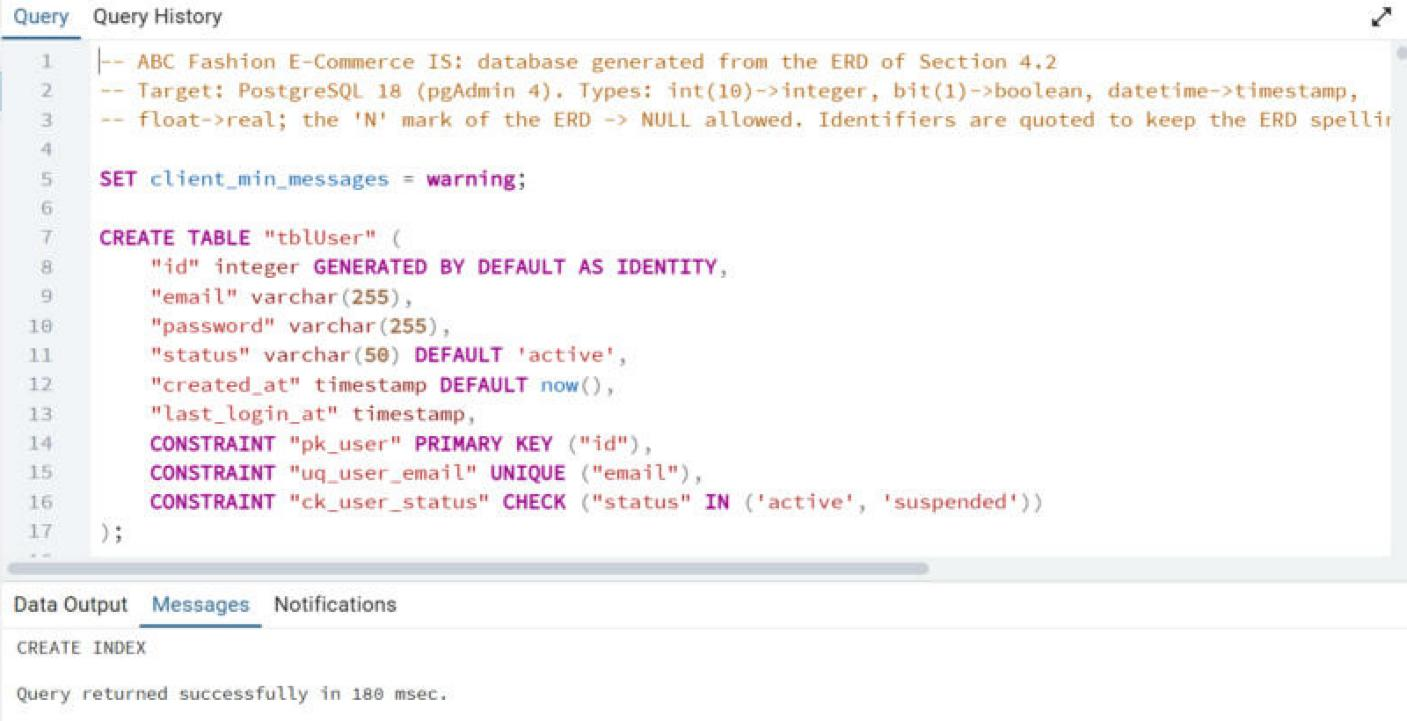
\includegraphics[width=0.95\textwidth]{db_ddl.png}
\caption{pgAdmin 4 --- the DDL script run in the Query Tool on database \texttt{abc\_fashion\_v2}}
\label{fig:dbddl}
\end{figure}

\subsection{Screens of the Database}
\label{subsec:dbscreens}
Figures~\ref{fig:dbpgerd}--\ref{fig:dbrule} are screen captures of the generated database in pgAdmin~4.

To check that the generated database has the structure of the ERD of Section~\ref{subsec:erd}, the ERD was also produced in the opposite direction: the \emph{ERD For Database} tool of pgAdmin~4 reads the 39 tables of schema \texttt{public} of \texttt{abc\_fashion\_v2} and draws them with their columns, data types, primary keys (key symbol), unique columns and foreign keys in crow's-foot notation (Figure~\ref{fig:dbpgerd}, parts in Figures~\ref{fig:dbpgerd1}--\ref{fig:dbpgerd4}). Every table, column and relationship of Figure~\ref{fig:erdfull} appears in it, e.g.\ \texttt{tblOrder}--\texttt{tblOrderItem} (one to many), \texttt{tblUser}--\texttt{tblCustomer} (one to one) and the junction tables \texttt{tblOrderVoucher} and \texttt{tblPromotionStyle}.

\begin{landscape}
\begin{figure}[p]
\centering
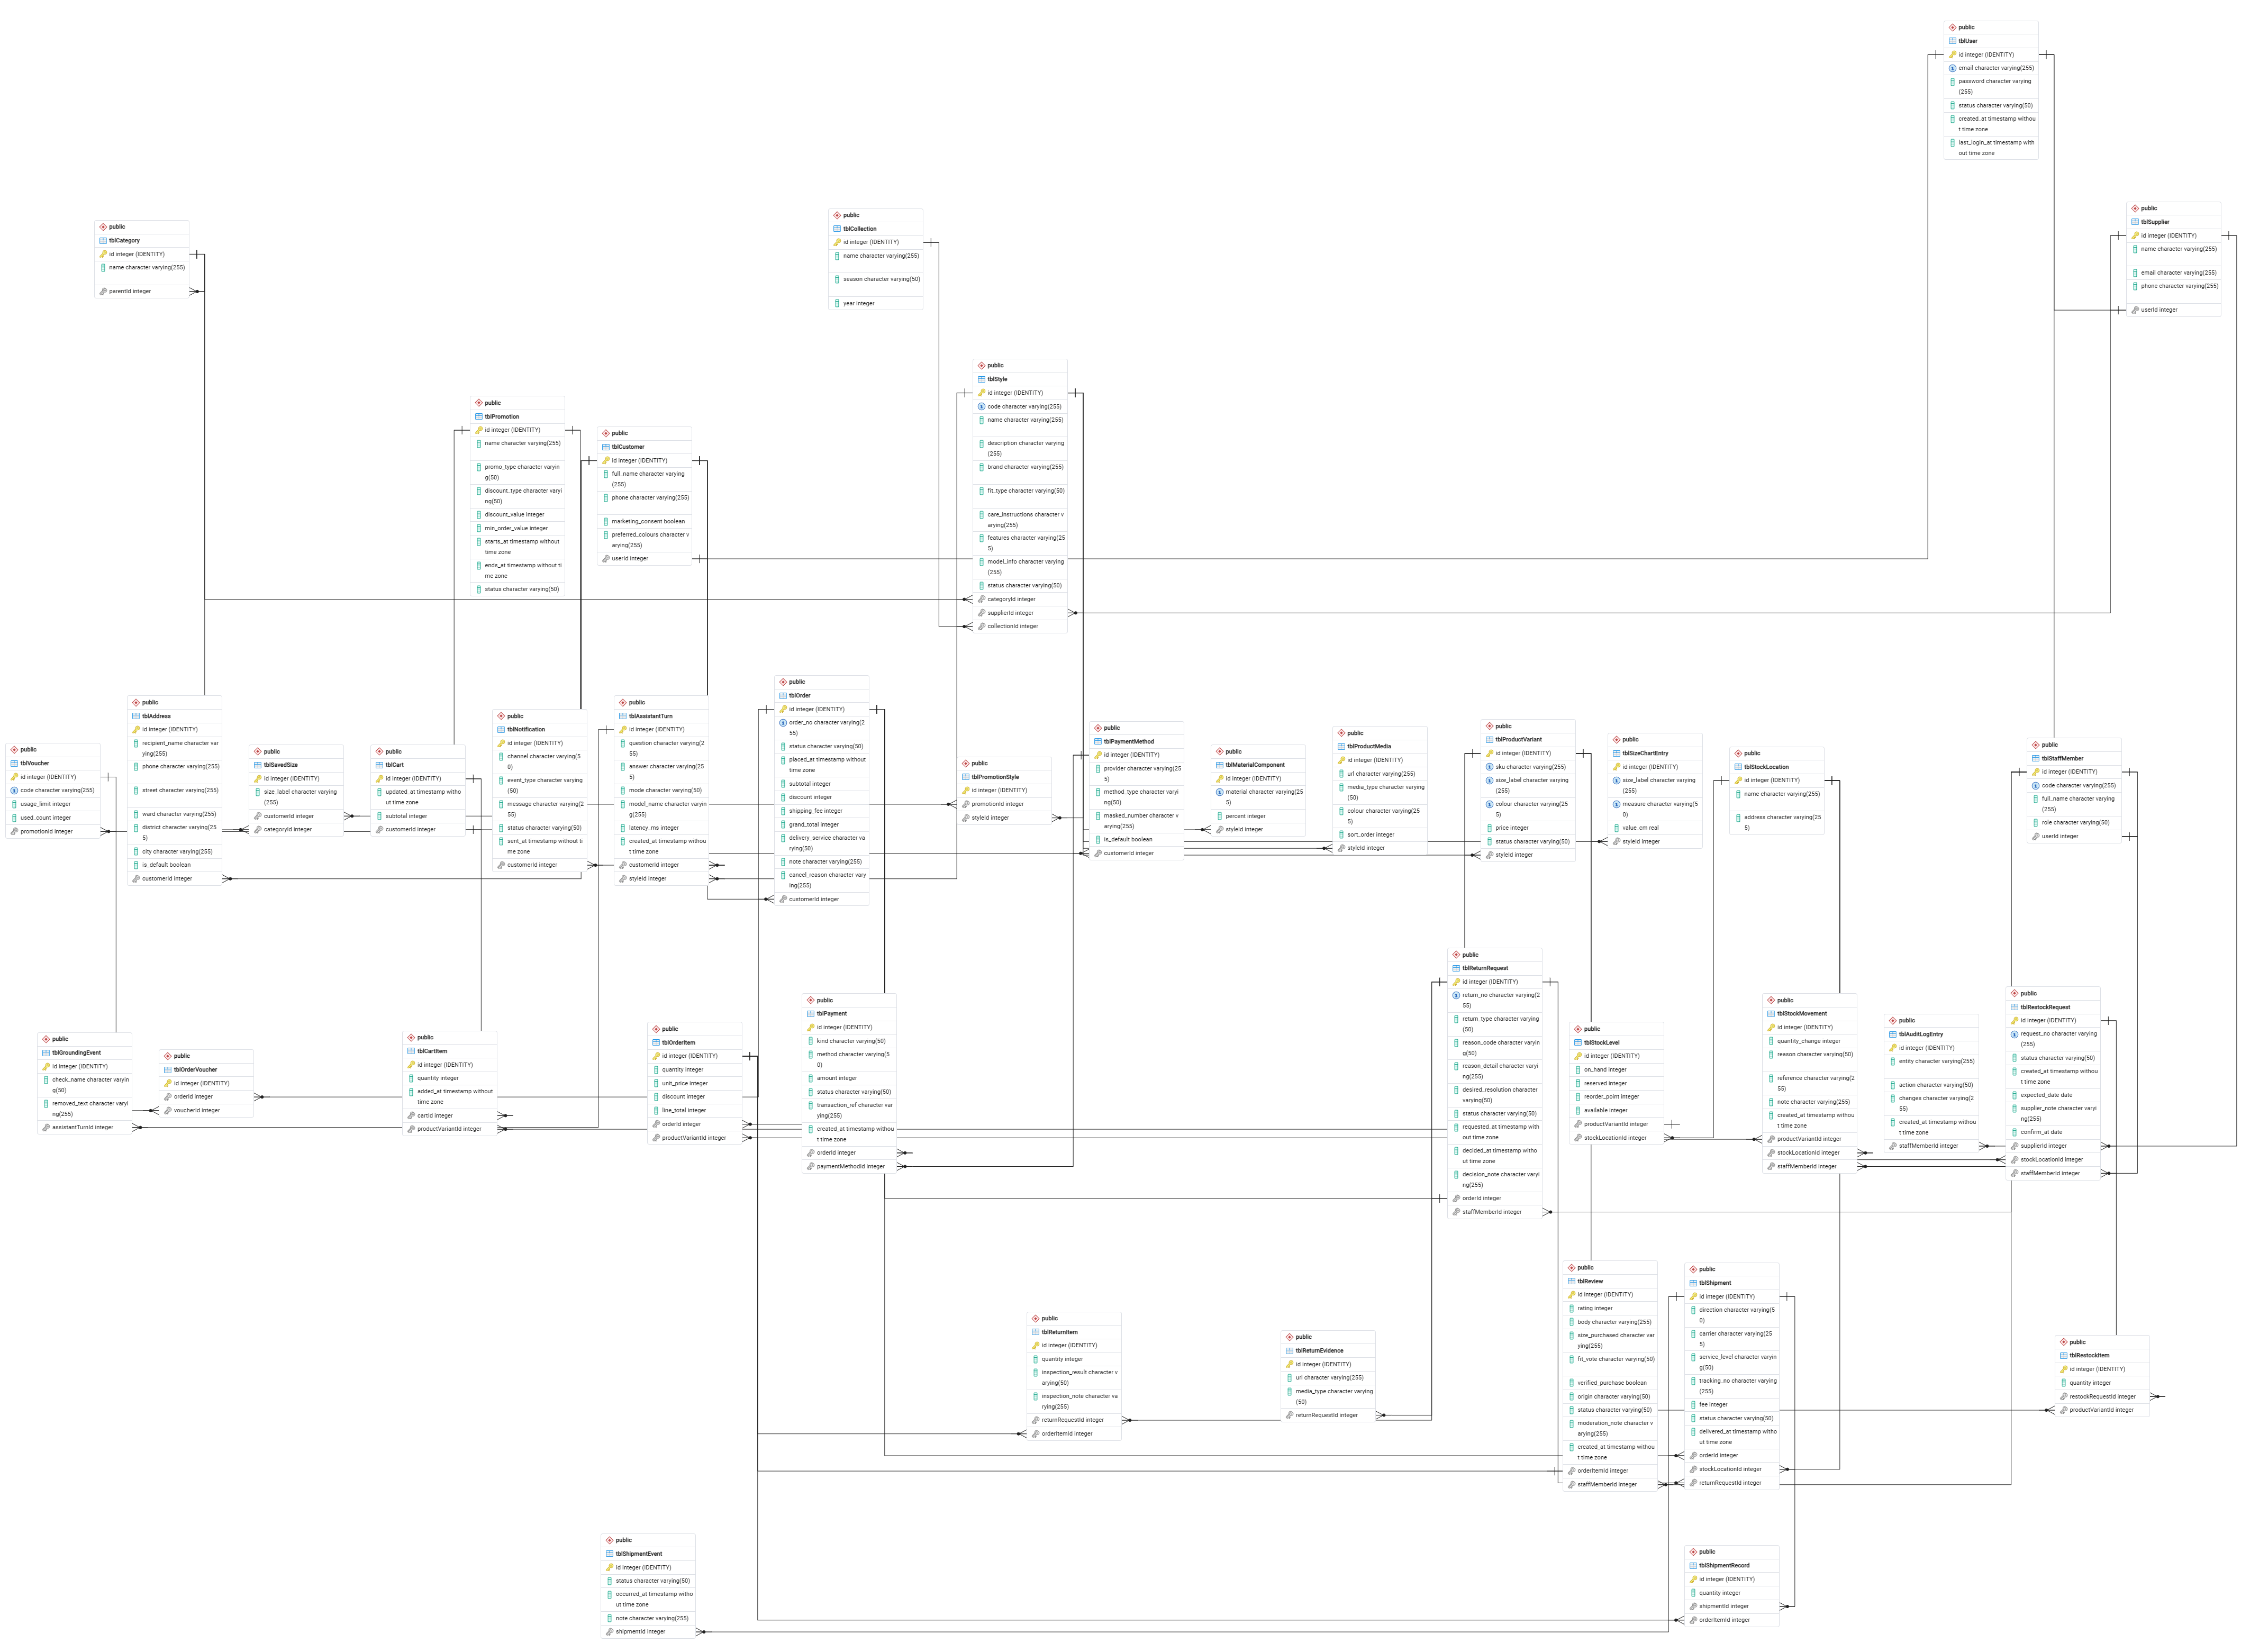
\includegraphics[width=\linewidth,height=0.88\textheight,keepaspectratio]{db_pgadmin_erd.png}
\caption{pgAdmin 4 --- ERD generated from database \texttt{abc\_fashion\_v2} (\emph{ERD For Database}): the 39 tables with their columns and foreign keys}
\label{fig:dbpgerd}
\end{figure}
\end{landscape}

\begin{figure}[H]
\centering
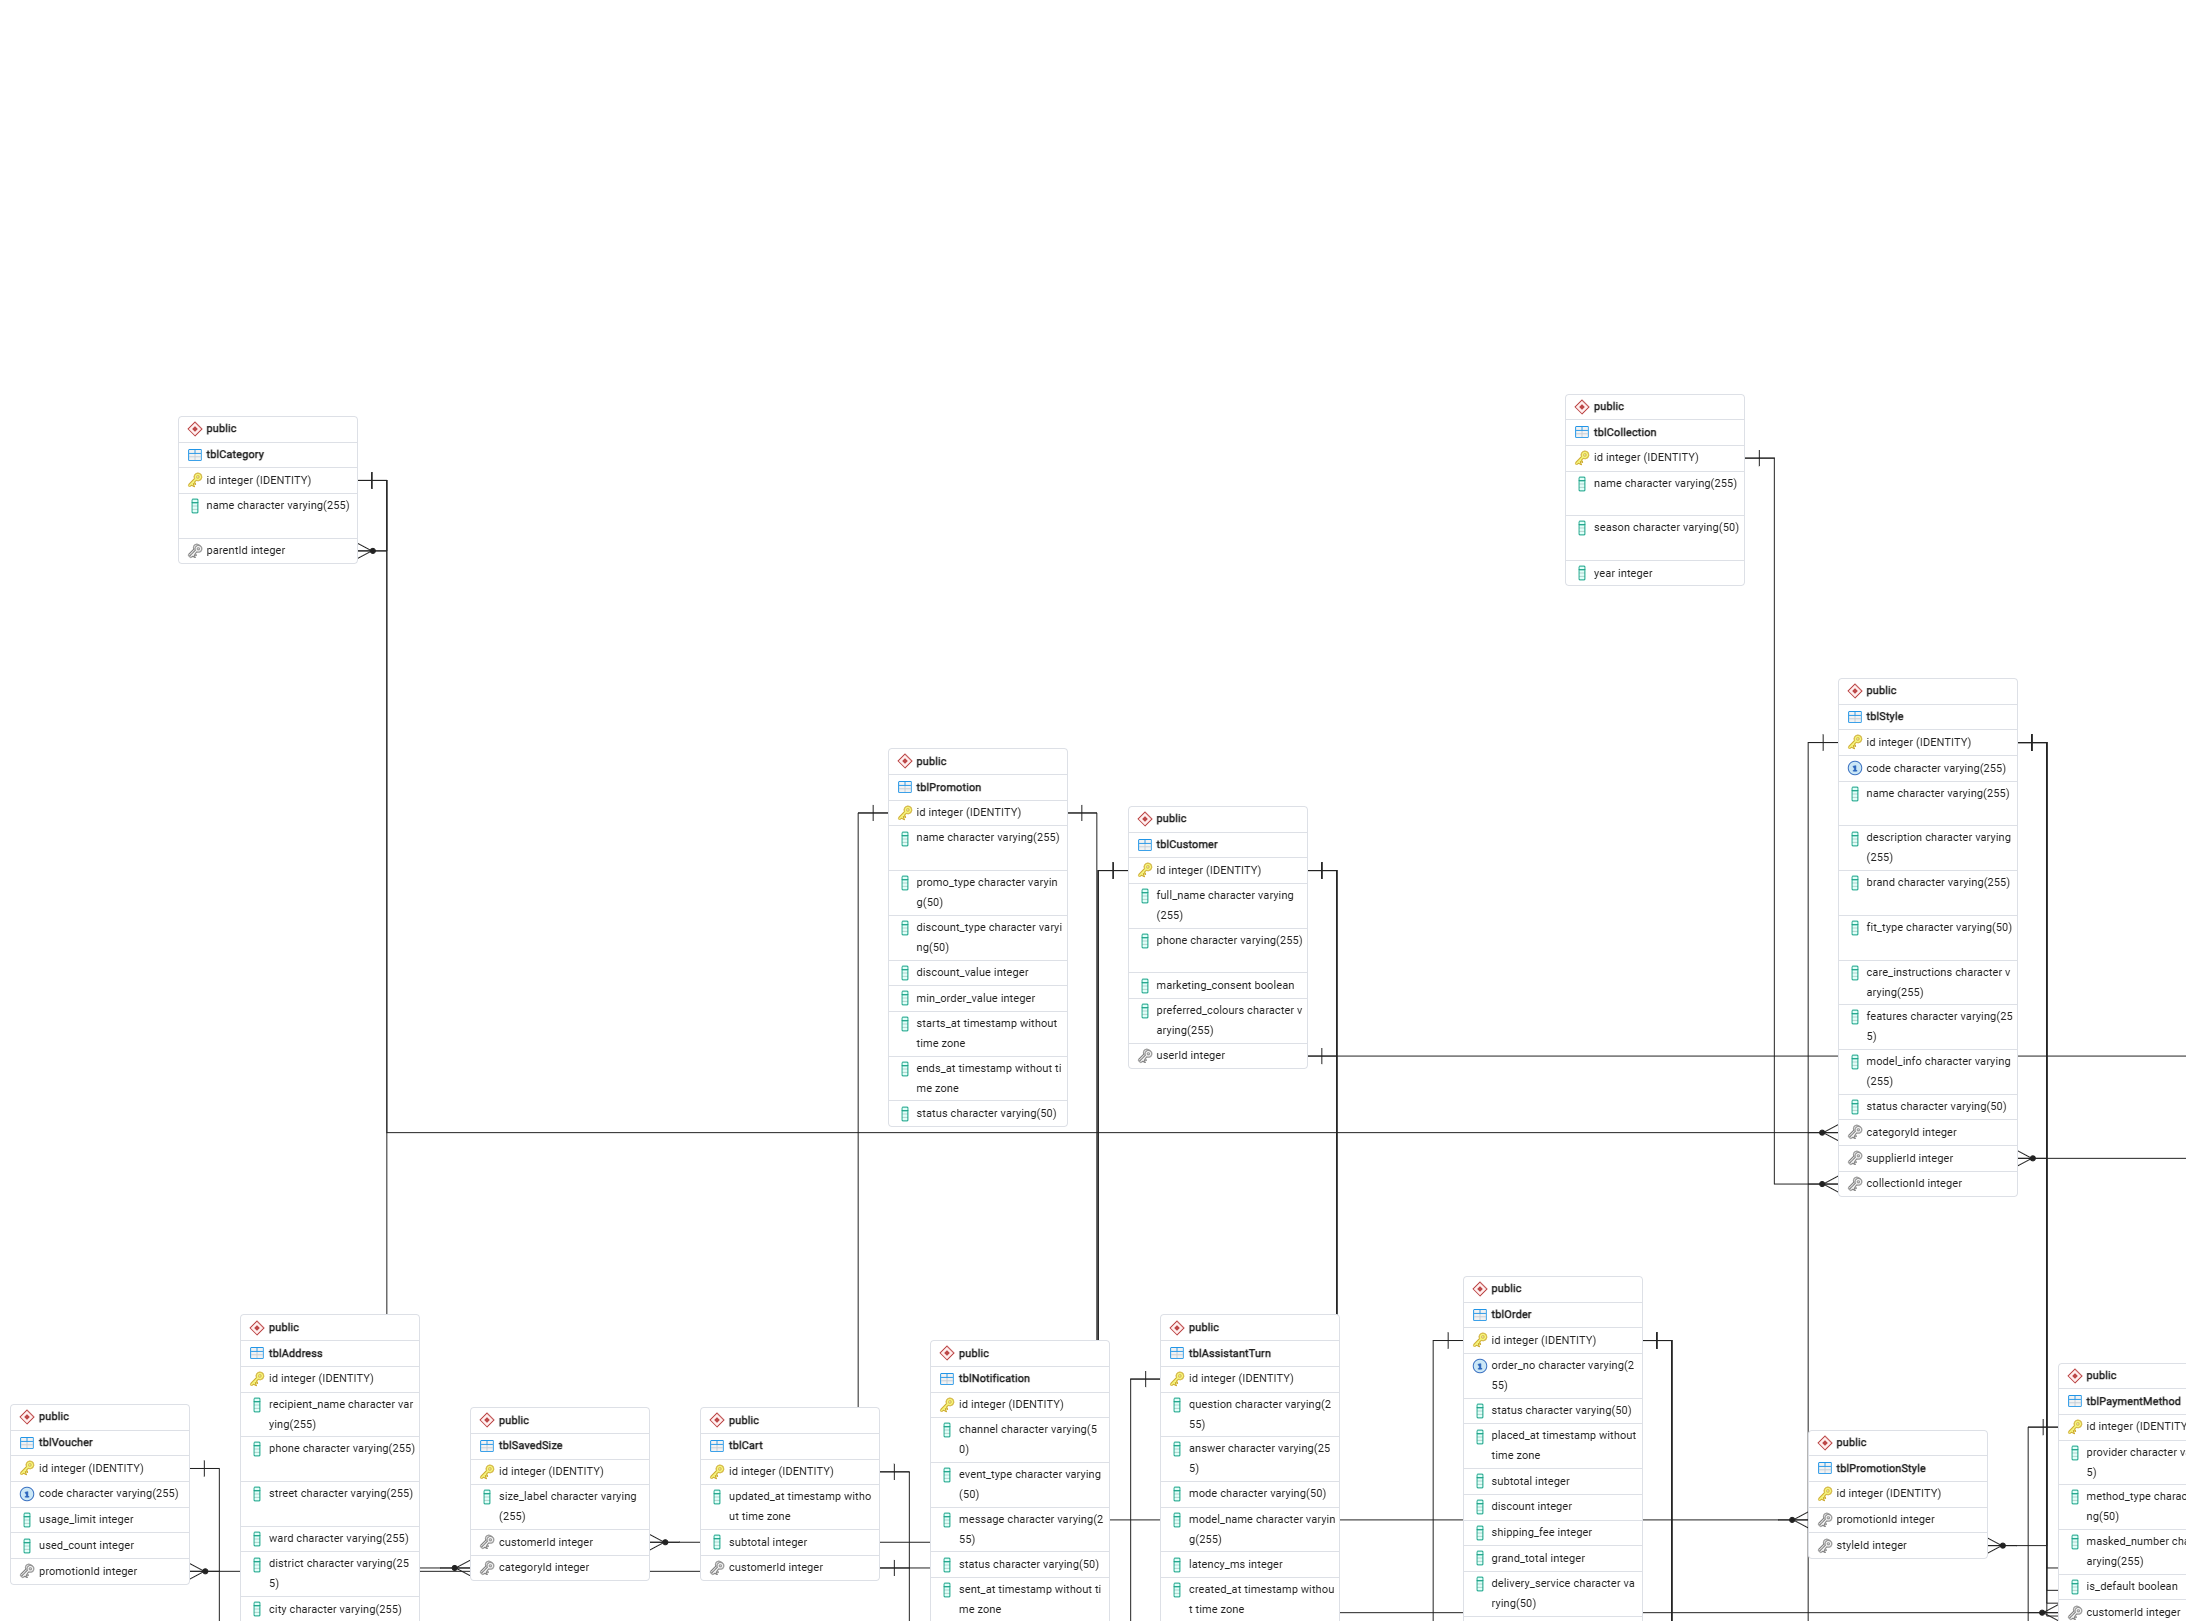
\includegraphics[width=\textwidth,height=0.75\textheight,keepaspectratio]{db_pgadmin_erd_p1.png}
\caption{ERD generated by pgAdmin 4, part 1 (upper left --- categories, promotions, customers, vouchers, addresses, carts, notifications and the assistant log)}
\label{fig:dbpgerd1}
\end{figure}

\begin{figure}[H]
\centering
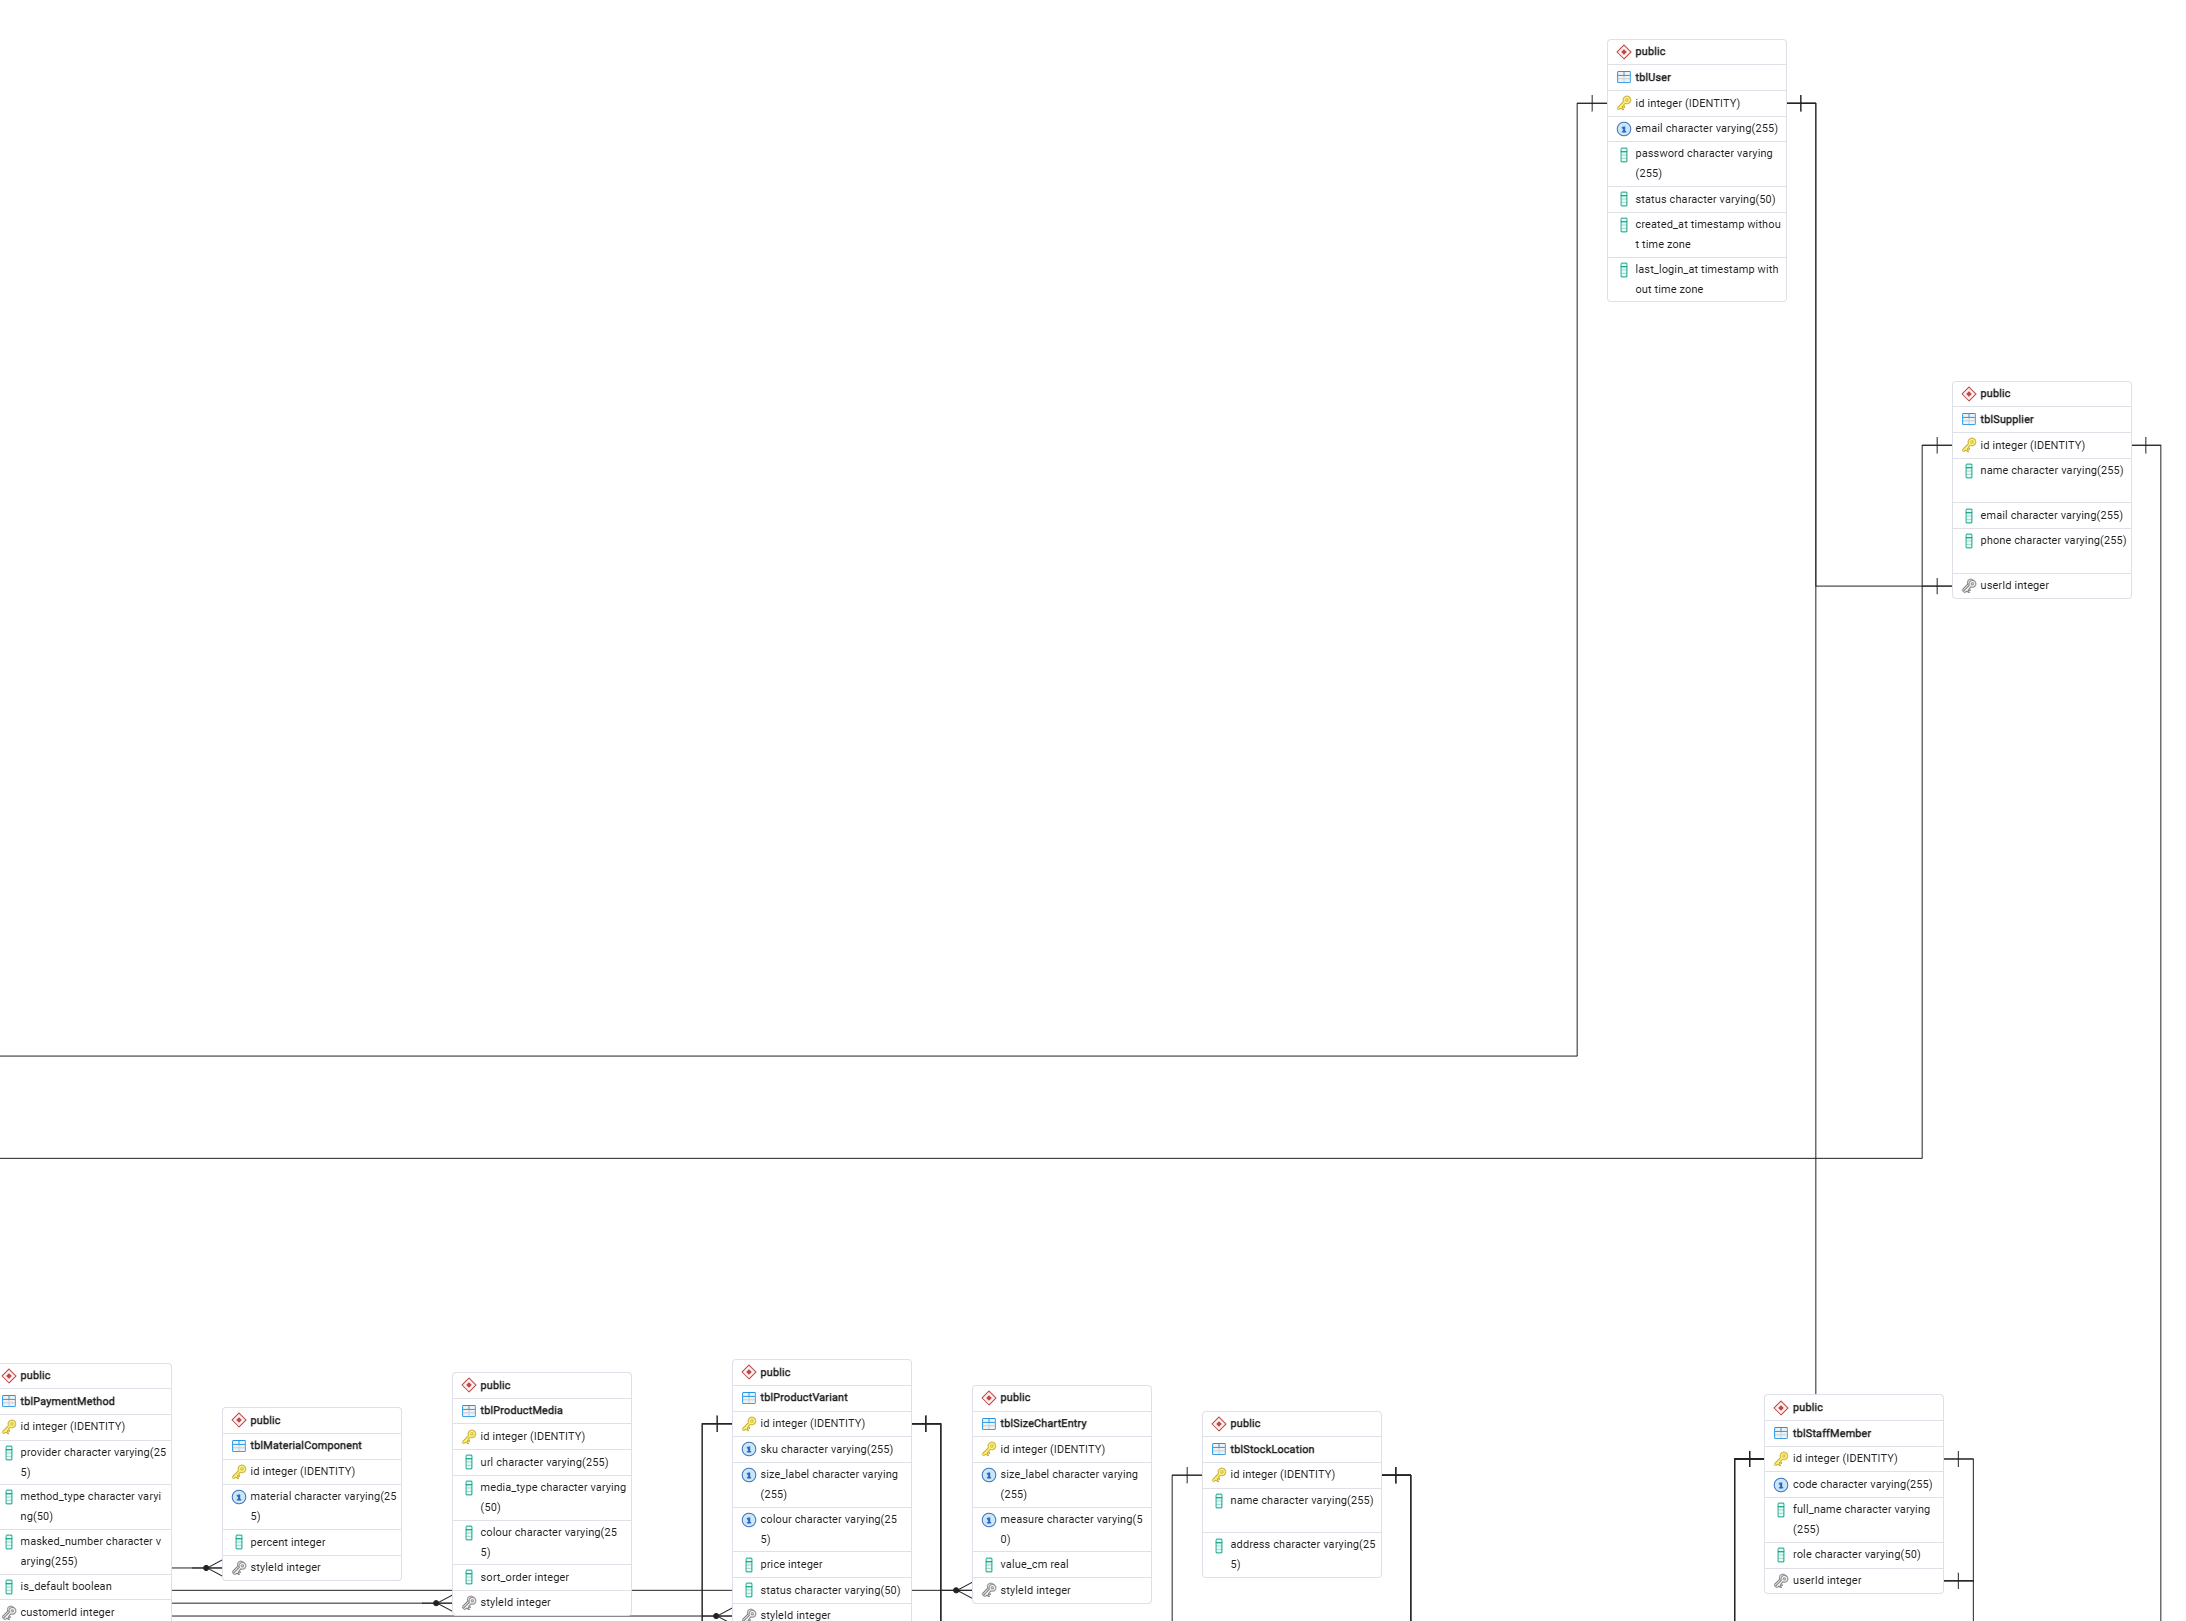
\includegraphics[width=\textwidth,height=0.75\textheight,keepaspectratio]{db_pgadmin_erd_p2.png}
\caption{ERD generated by pgAdmin 4, part 2 (upper right --- collections, styles, users, suppliers, payment methods, media, variants, size charts, stock locations and staff)}
\label{fig:dbpgerd2}
\end{figure}

\begin{figure}[H]
\centering
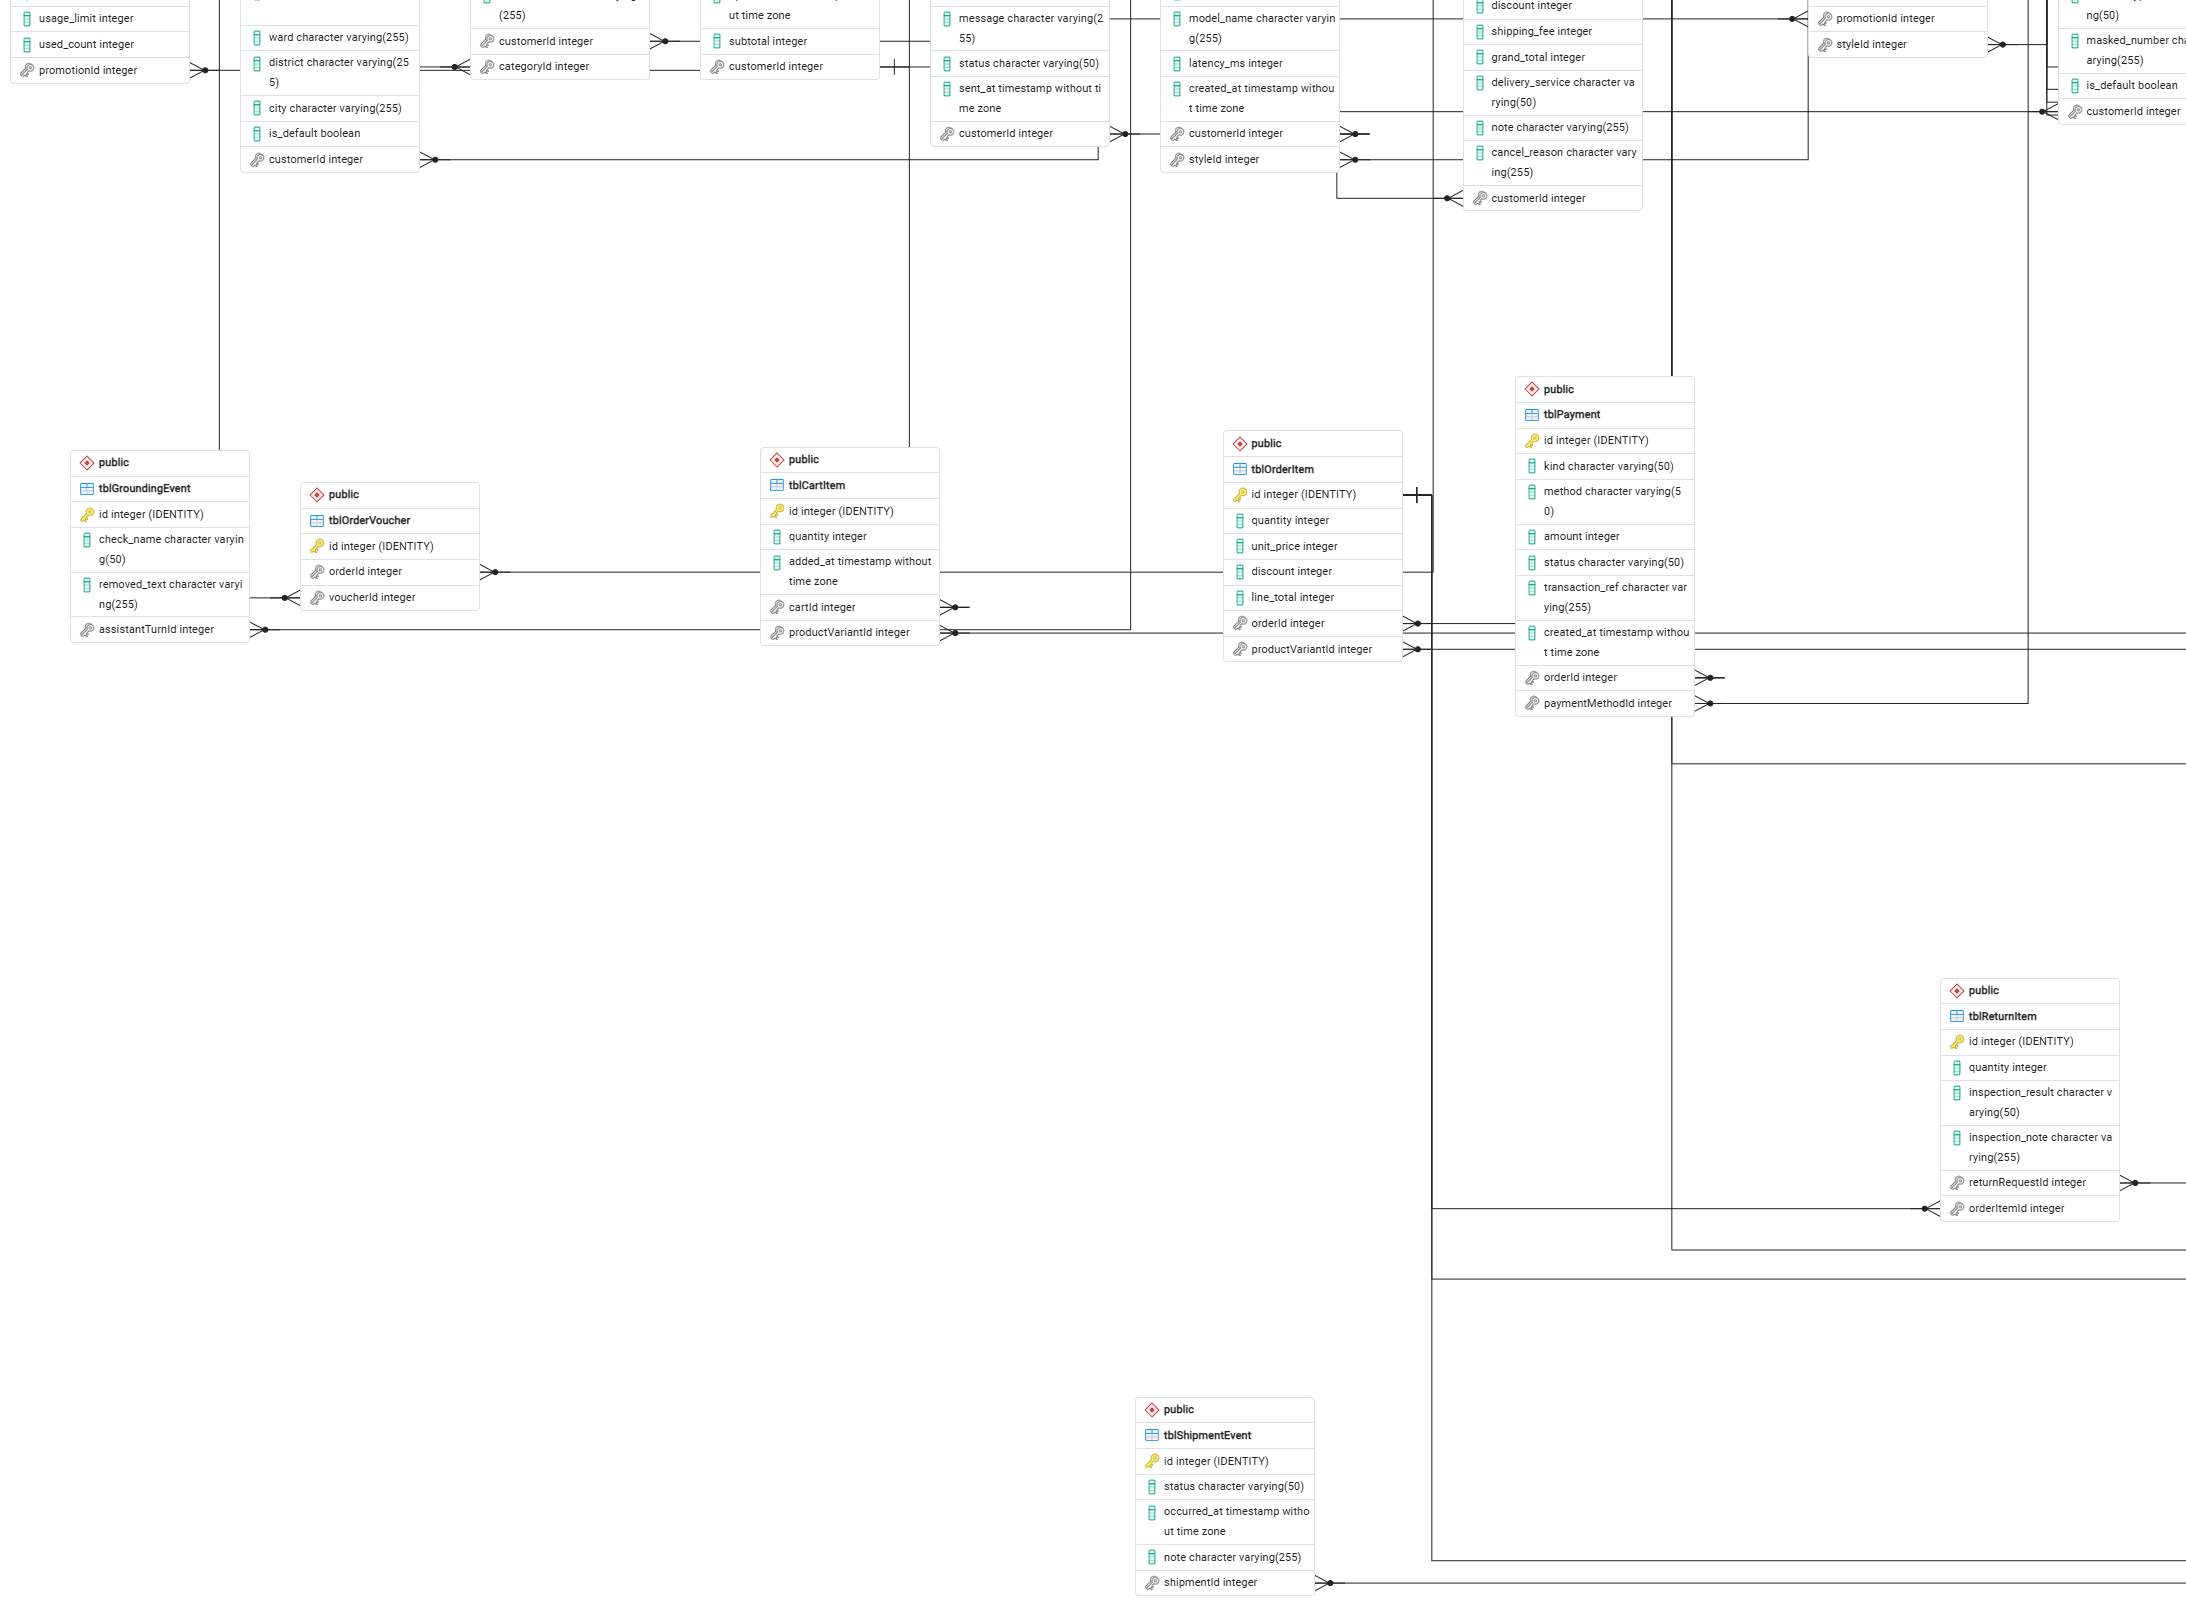
\includegraphics[width=\textwidth,height=0.75\textheight,keepaspectratio]{db_pgadmin_erd_p3.png}
\caption{ERD generated by pgAdmin 4, part 3 (lower left --- grounding events, order vouchers, cart items, order items, payments, return items and shipment events)}
\label{fig:dbpgerd3}
\end{figure}

\begin{figure}[H]
\centering
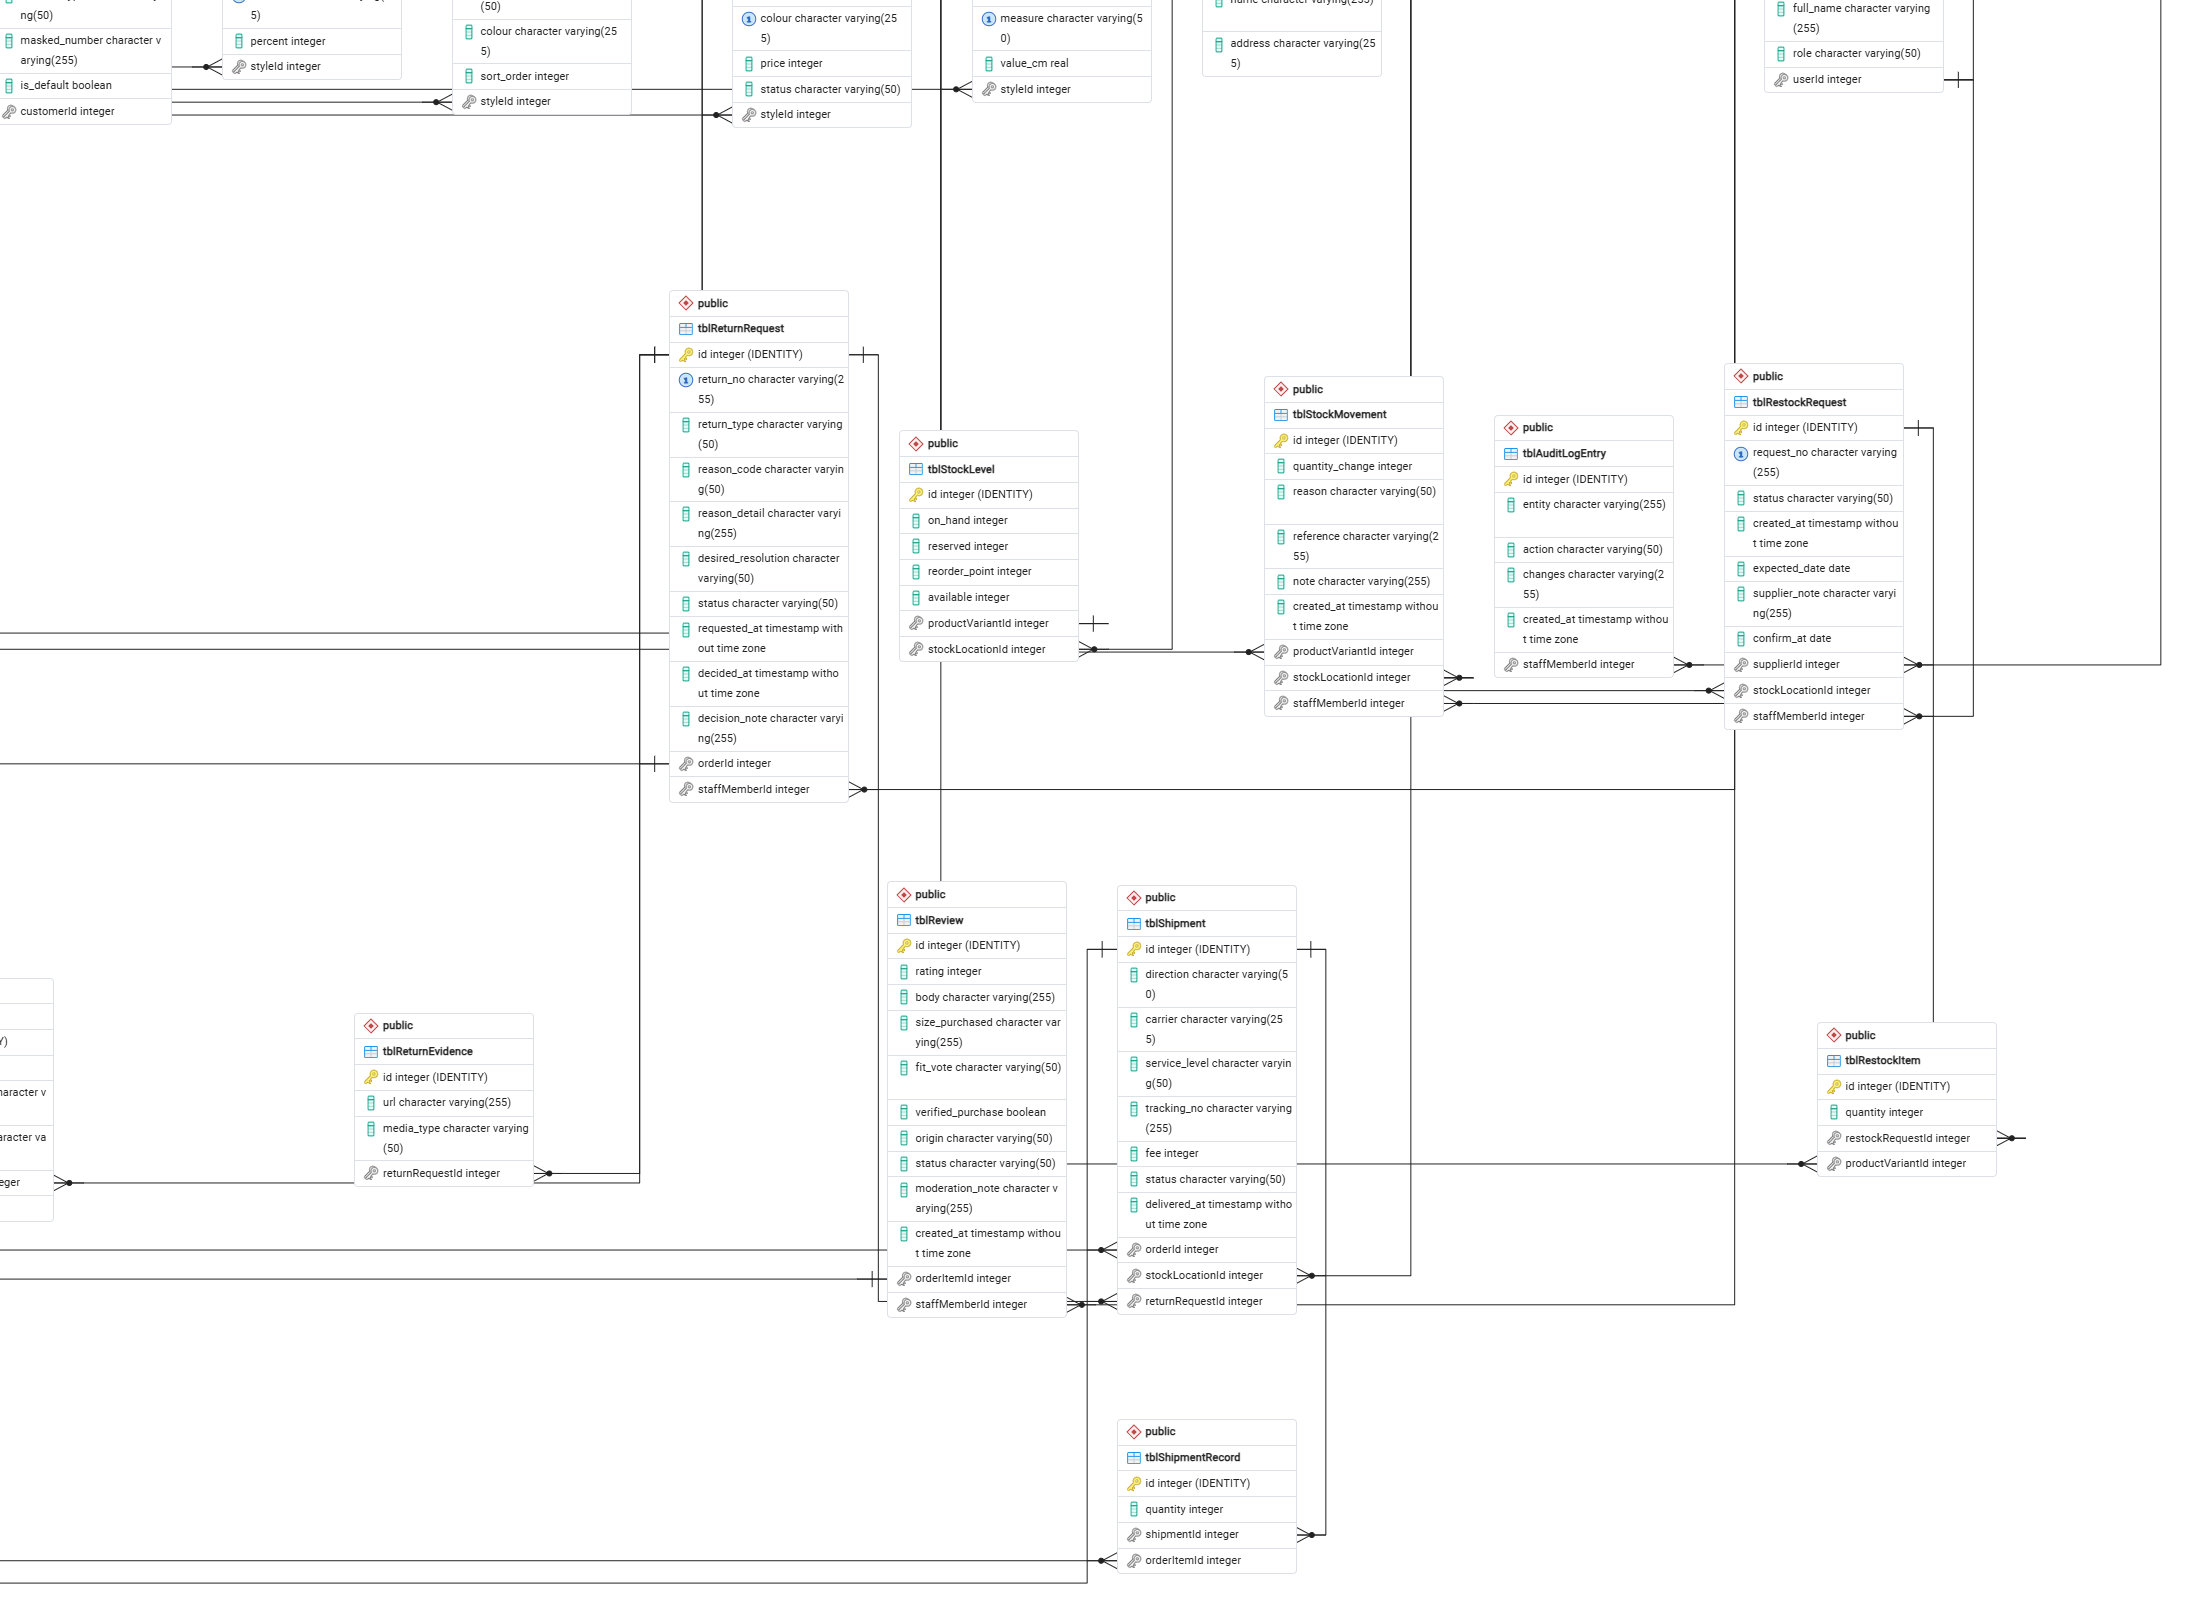
\includegraphics[width=\textwidth,height=0.75\textheight,keepaspectratio]{db_pgadmin_erd_p4.png}
\caption{ERD generated by pgAdmin 4, part 4 (lower right --- return requests, stock levels and movements, audit log, restocking, reviews, shipments and shipment records)}
\label{fig:dbpgerd4}
\end{figure}


\begin{figure}[H]
\centering
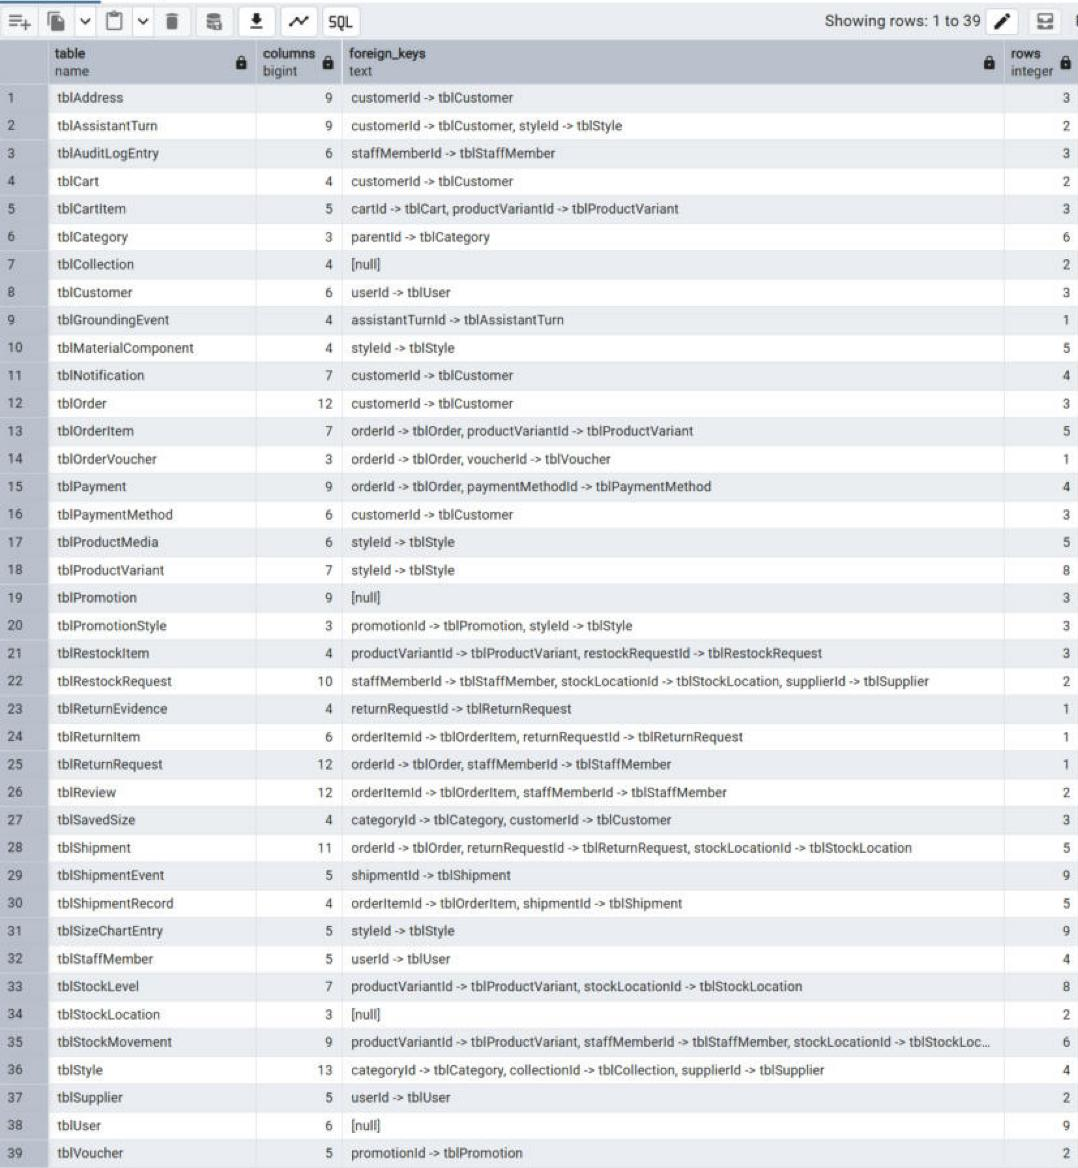
\includegraphics[width=0.92\textwidth,height=0.78\textheight,keepaspectratio]{db_tables.png}
\caption{pgAdmin 4 --- the 39 tables of \texttt{abc\_fashion\_v2} with their number of columns, their foreign keys and their number of rows (query on the system catalogue)}
\label{fig:dbtables}
\end{figure}

\begin{figure}[H]
\centering
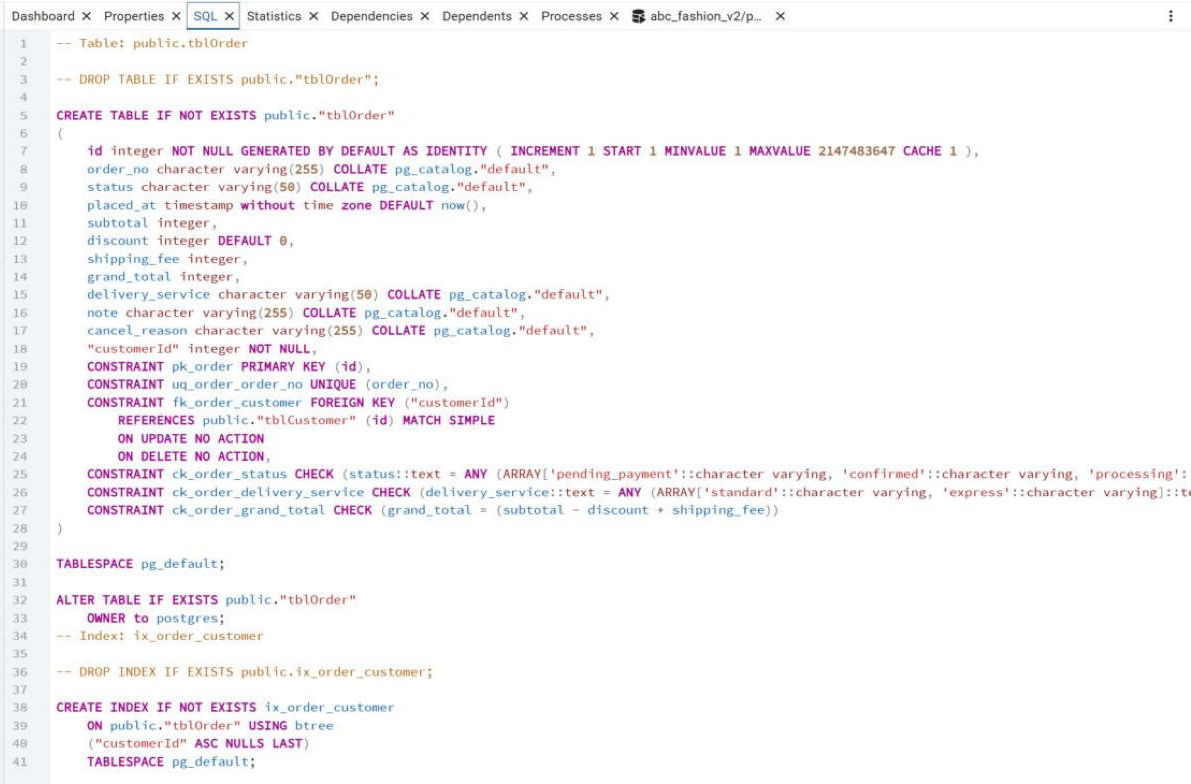
\includegraphics[width=\textwidth]{db_order_sql.png}
\caption{pgAdmin 4 --- structure of \texttt{tblOrder} as stored in the database: columns, primary key, unique key, foreign key to \texttt{tblCustomer}, check constraints and index}
\label{fig:dborder}
\end{figure}

\begin{figure}[H]
\centering
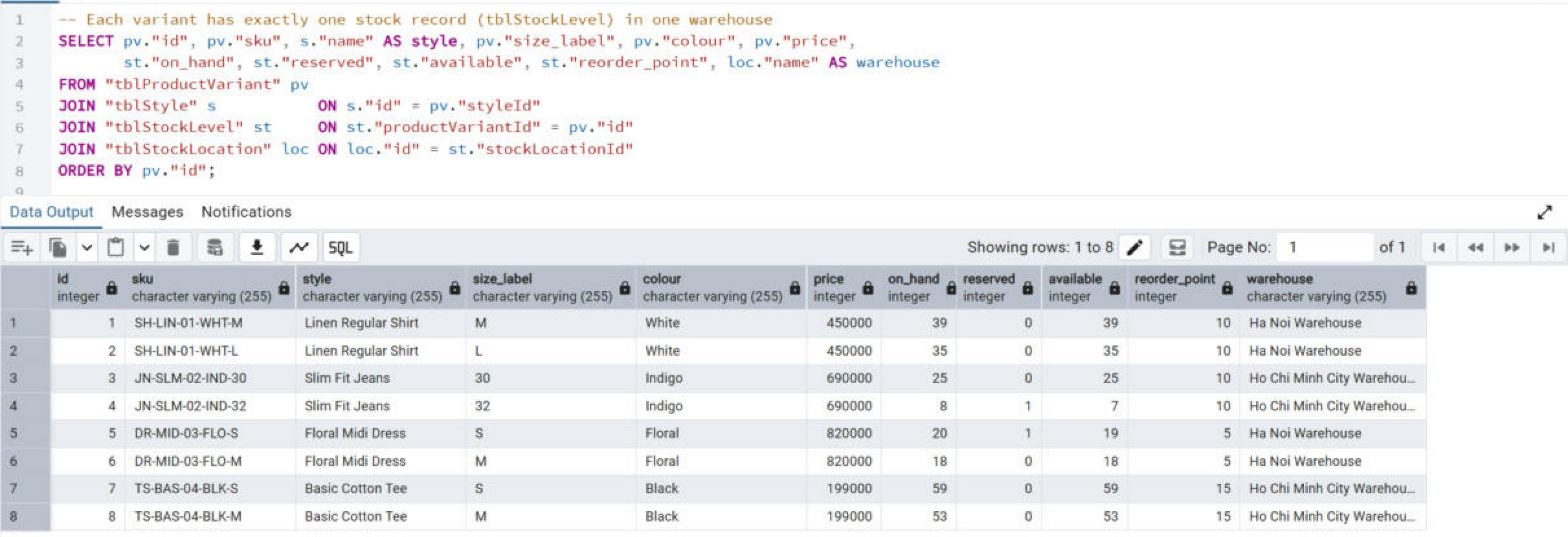
\includegraphics[width=\textwidth]{db_stock.png}
\caption{pgAdmin 4 --- the eight variants with their single stock record and warehouse (\texttt{tblProductVariant}, \texttt{tblStyle}, \texttt{tblStockLevel}, \texttt{tblStockLocation})}
\label{fig:dbstock}
\end{figure}

\begin{figure}[H]
\centering
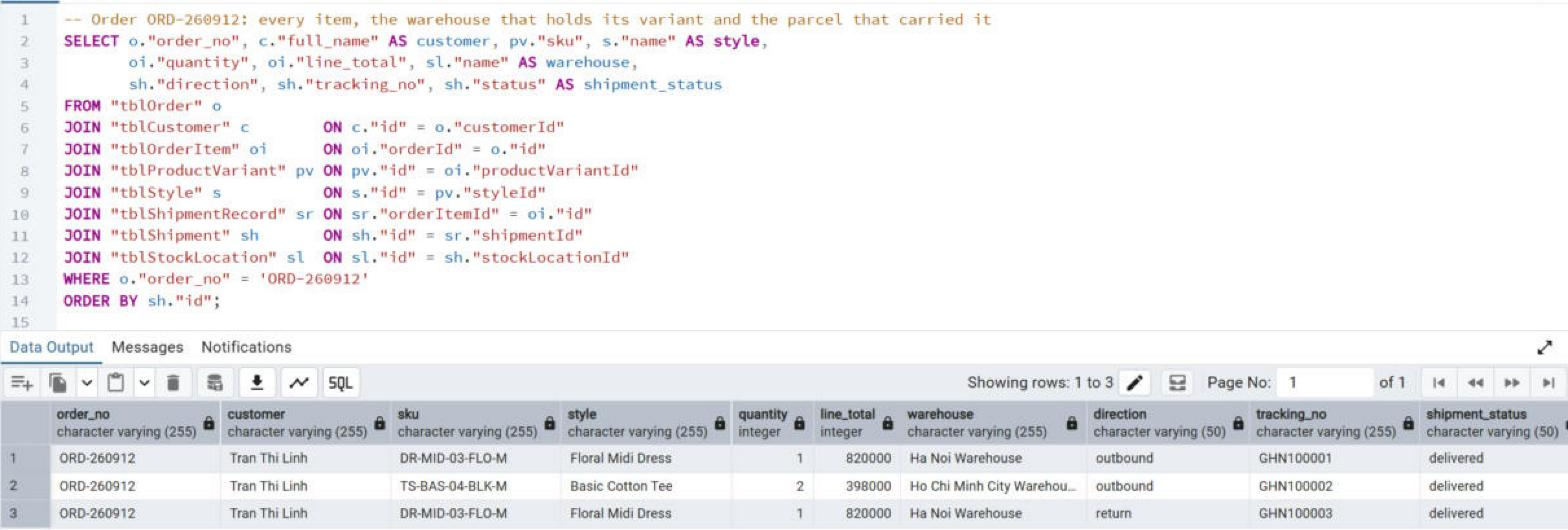
\includegraphics[width=\textwidth]{db_join.png}
\caption{pgAdmin 4 --- query over eight tables: order ORD-260912 is split into two parcels, one from each warehouse, and the dress comes back in a return parcel}
\label{fig:dbjoin}
\end{figure}

\begin{figure}[H]
\centering
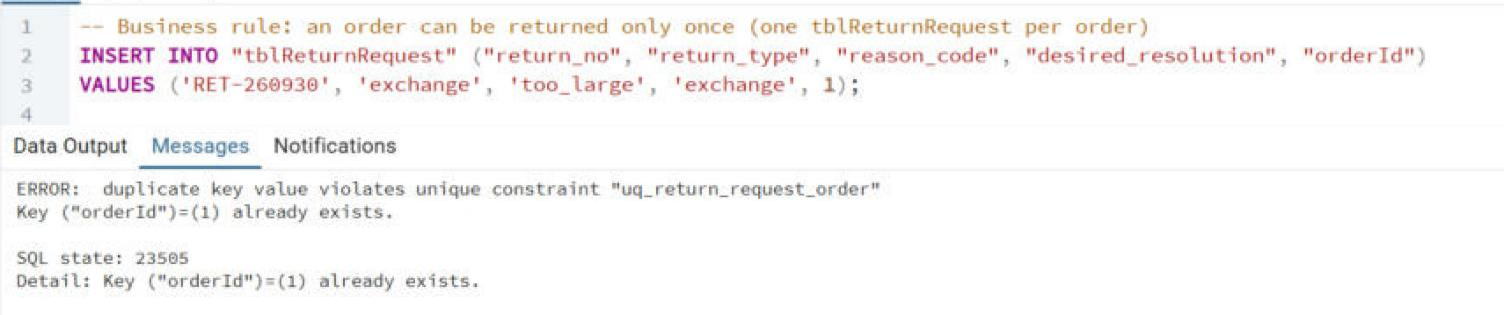
\includegraphics[width=\textwidth]{db_rule.png}
\caption{pgAdmin 4 --- the database rejects a second return request for the same order (constraint \texttt{uq\_return\_request\_order})}
\label{fig:dbrule}
\end{figure}

% =====================================================================
\section{Class Diagram in Design}
\label{sec:designclass}

The design class diagram turns the analysis model of Section~\ref{sec:analysisclass} and the tables of Section~\ref{sec:datamodel} into classes that can be programmed in Python. It follows the Model--View--Controller (MVC) style \cite{dennis2020}: each screen of the user interface is a \emph{view} class; a \emph{controller} class receives the requests of a group of screens, applies the business rules and coordinates the work; the \emph{model} holds the data and the access to it --- the \emph{entity} classes carry the data, one \emph{data-access} (DAO) class per table holds the SQL, and five \emph{gateway} classes reach the external services. A view never calls a DAO or a gateway directly; it only calls its controller. The diagram was drawn in Visual Paradigm (Figure~\ref{fig:designfull}).

\subsection{From Analysis to Design}
\label{subsec:refinement}
Table~\ref{tab:refinements} summarises the decisions that turn the analysis classes into design classes.

{\small
\begin{xltabular}{\textwidth}{@{}L{3.6cm} Y@{}}
\caption{Design decisions applied to the analysis model}\label{tab:refinements}\\
\toprule
\textbf{Decision} & \textbf{Rule and example} \\ \midrule
\endfirsthead
\toprule
\textbf{Decision} & \textbf{Rule and example} \\ \midrule
\endhead
\bottomrule
\endlastfoot
Kinds of class & \textbf{Entity} classes carry data (one per table, named with the analysis name of the class: \textsf{Order} for table \texttt{tblOrder}; the prefix \texttt{tbl} is used only for the tables of the database); \textbf{view} classes are screens (suffix \textsf{Frm}: \textsf{CheckoutFrm}); \textbf{controller} classes carry out the use cases (suffix \textsf{Controller}: \textsf{CheckoutController}); \textbf{DAO} classes read and write the database (suffix \textsf{DAO}: \textsf{OrderDAO}); \textbf{gateway} classes call the external services (\textsf{PaymentGateway}). A view never contains SQL or business rules, a controller never shows anything, and a DAO never decides anything. \\
Entity = row of a table & Each entity class has exactly the columns of its table in Section~\ref{sec:datamodel}, including the surrogate key \texttt{id} and the foreign keys (\texttt{customerId}, \ldots). Attributes are private (\texttt{-}) and typed with the Python types of Table~\ref{tab:typemapping}; columns with a fixed list of values are typed with the enumeration (\texttt{status: OrderStatus}). \\
Packages & Every entity is placed in a package together with the enumerations it uses, joined by \guillemotleft use\guillemotright{} dependencies, exactly as in the analysis diagram. \\
Relationships kept & Generalisations (\textsf{User} $\leftarrow$ \textsf{Customer}, \textsf{StaffMember}, \textsf{Supplier}; \textsf{ProductVariant} $\leftarrow$ \textsf{CartItem} $\leftarrow$ \textsf{OrderItem} $\leftarrow$ \textsf{ReturnItem}), compositions and aggregations with their multiplicities are copied from the analysis model; the two junction tables appear as the classes \textsf{OrderVoucher} and \textsf{PromotionStyle}. \\
One view per screen & Each step of a use case that shows a screen becomes one \textsf{Frm} class. Its attributes are the user-interface components (\texttt{txt\_} entry, \texttt{btn\_} button, \texttt{tbl\_} table, \texttt{cbo\_} combo box, \texttt{lbl\_} label, \ldots{} of the Python library \texttt{tkinter.ttk}) and the entity objects it shows or passes on; its operations are the constructor \texttt{\_\_init\_\_} and one handler \texttt{on\_<action>} per button. \\
One controller per group of use cases & The use cases of one business area are realised by one controller class (15 in all, Table~\ref{tab:controllers}): it checks the input, runs the operations that change several tables in one transaction through the DAOs, calls the gateways outside the transaction and sends the notifications. A controller knows neither \texttt{tkinter} nor the web framework, so the desktop screens and the customer web application use the same controllers. \\
One DAO per table & Every table that a controller reads or writes has a data-access class \textsf{XxxDAO} whose operations are named verb + entity (\texttt{search\_style}, \texttt{add\_order}). All DAO classes inherit the class \textsf{DAO}, which only opens the connection to PostgreSQL. A DAO has operations only, no attributes. \\
Report data & The two reports need values that are computed, not stored (quantity sold, return rate); \textsf{StyleStatDAO} and \textsf{ReturnStatDAO} return them as statistic objects \textsf{StyleStat} and \textsf{ReturnStat} (a style with extra figures). \\
Python conventions & Class names in \texttt{CamelCase}, attributes and operations in \texttt{snake\_case}, \texttt{self} as first parameter, optional values as \texttt{X \textbar{} None}, lists as \texttt{list[X]}. \\
\end{xltabular}
}

\subsection{The Design Class Diagram}
\label{subsec:designdiagrams}
The complete diagram contains \textbf{182 classes} with \textbf{459 operations}: 53 view classes, 15 controller classes, 34 DAO classes (33 and the base class \textsf{DAO}), 5 gateway classes, 41 entity classes (39 tables and the two statistic classes \textsf{StyleStat} and \textsf{ReturnStat}) and the 34 enumerations used by the entities. Figure~\ref{fig:designfull} shows it as a whole. It is arranged in four bands --- the views at the top, the controllers below them, then the package \texttt{control} with the gateways and the DAO classes, and the entity packages at the bottom --- so that every line runs downwards: from a view to a controller, from a controller to a DAO or a gateway, and from a DAO to its entity. There is no line from a view to a DAO, a gateway or an entity: a screen keeps its data in typed attributes (\texttt{CheckoutFrm.customer: Customer}) and receives entities as parameters, and the package dependency \texttt{view} $\rightarrow$ \texttt{model} (Figure~\ref{fig:layers}) records this use, so the diagram does not repeat it line by line. Figures~\ref{fig:design1}--\ref{fig:design7} show the bands at a readable size.

\begin{landscape}
\begin{figure}[p]
\centering
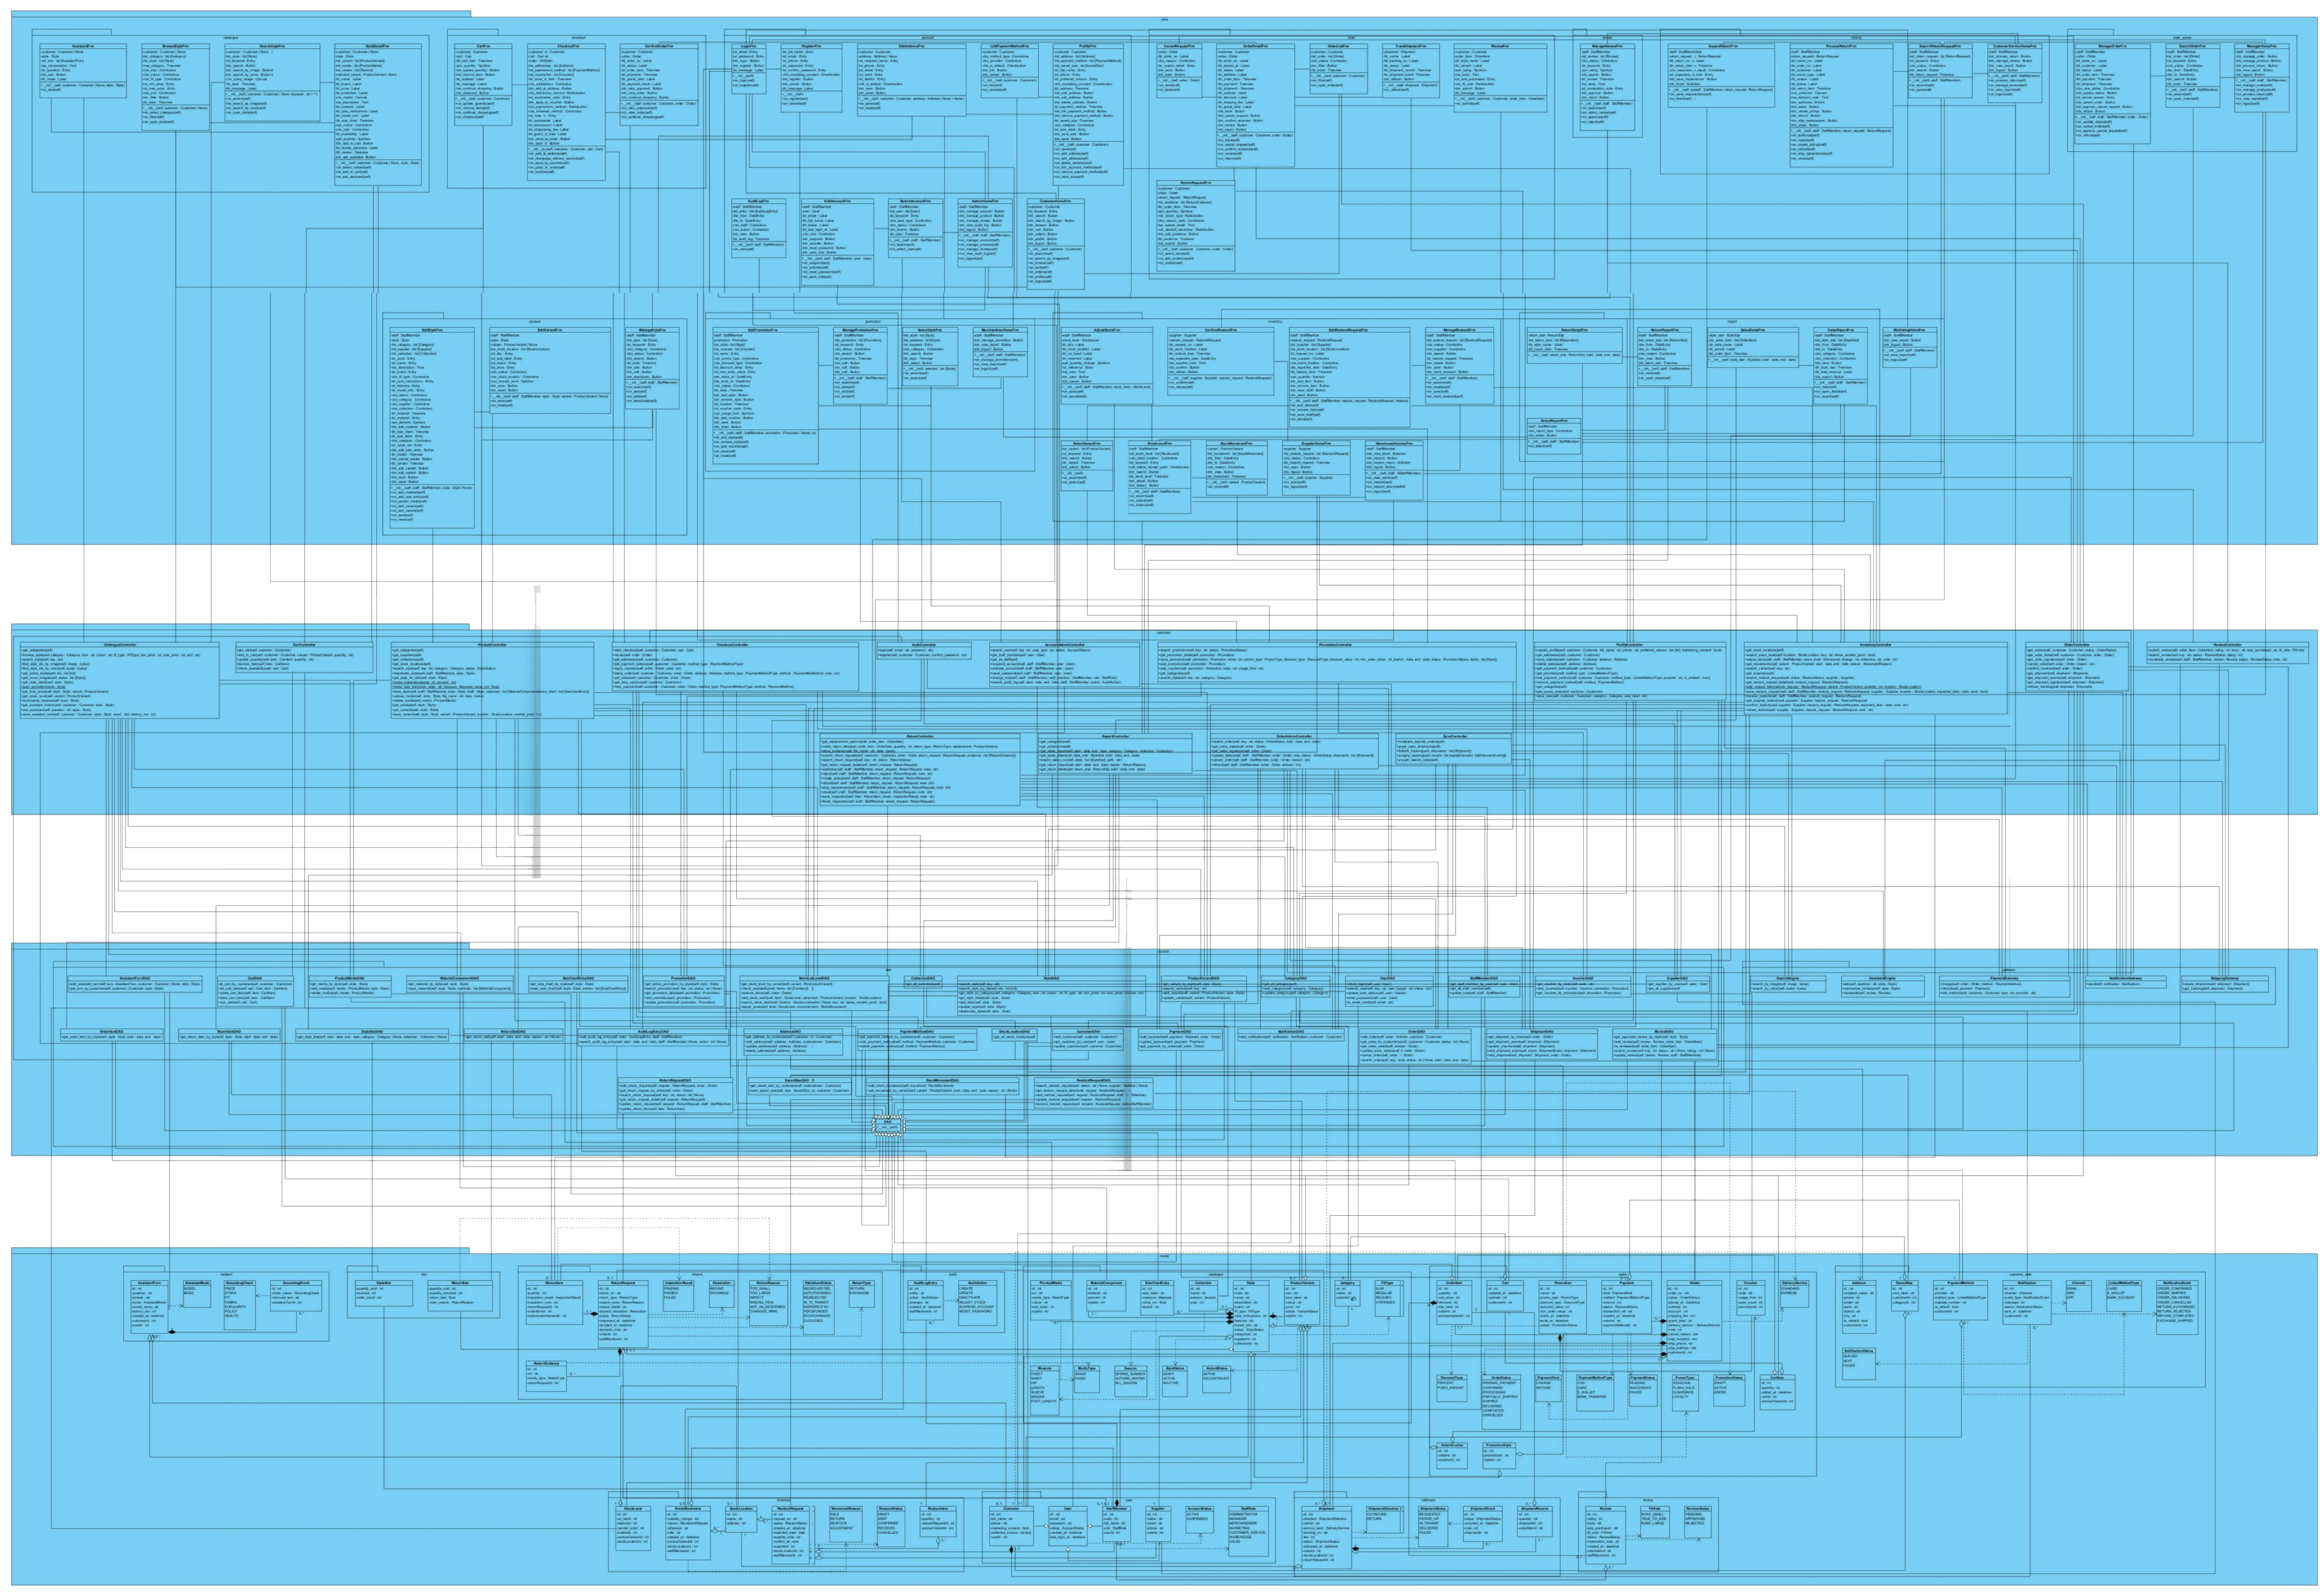
\includegraphics[width=\linewidth,height=0.92\textheight,keepaspectratio]{dc_full.jpg}
\caption{Design class diagram of the ABC Fashion E-Commerce Information System (Visual Paradigm): view classes (top), controller classes, the \texttt{control} package with the gateway and DAO classes, and the entity classes (bottom)}
\label{fig:designfull}
\end{figure}
\end{landscape}

\begin{landscape}
\begin{figure}[p]
\centering
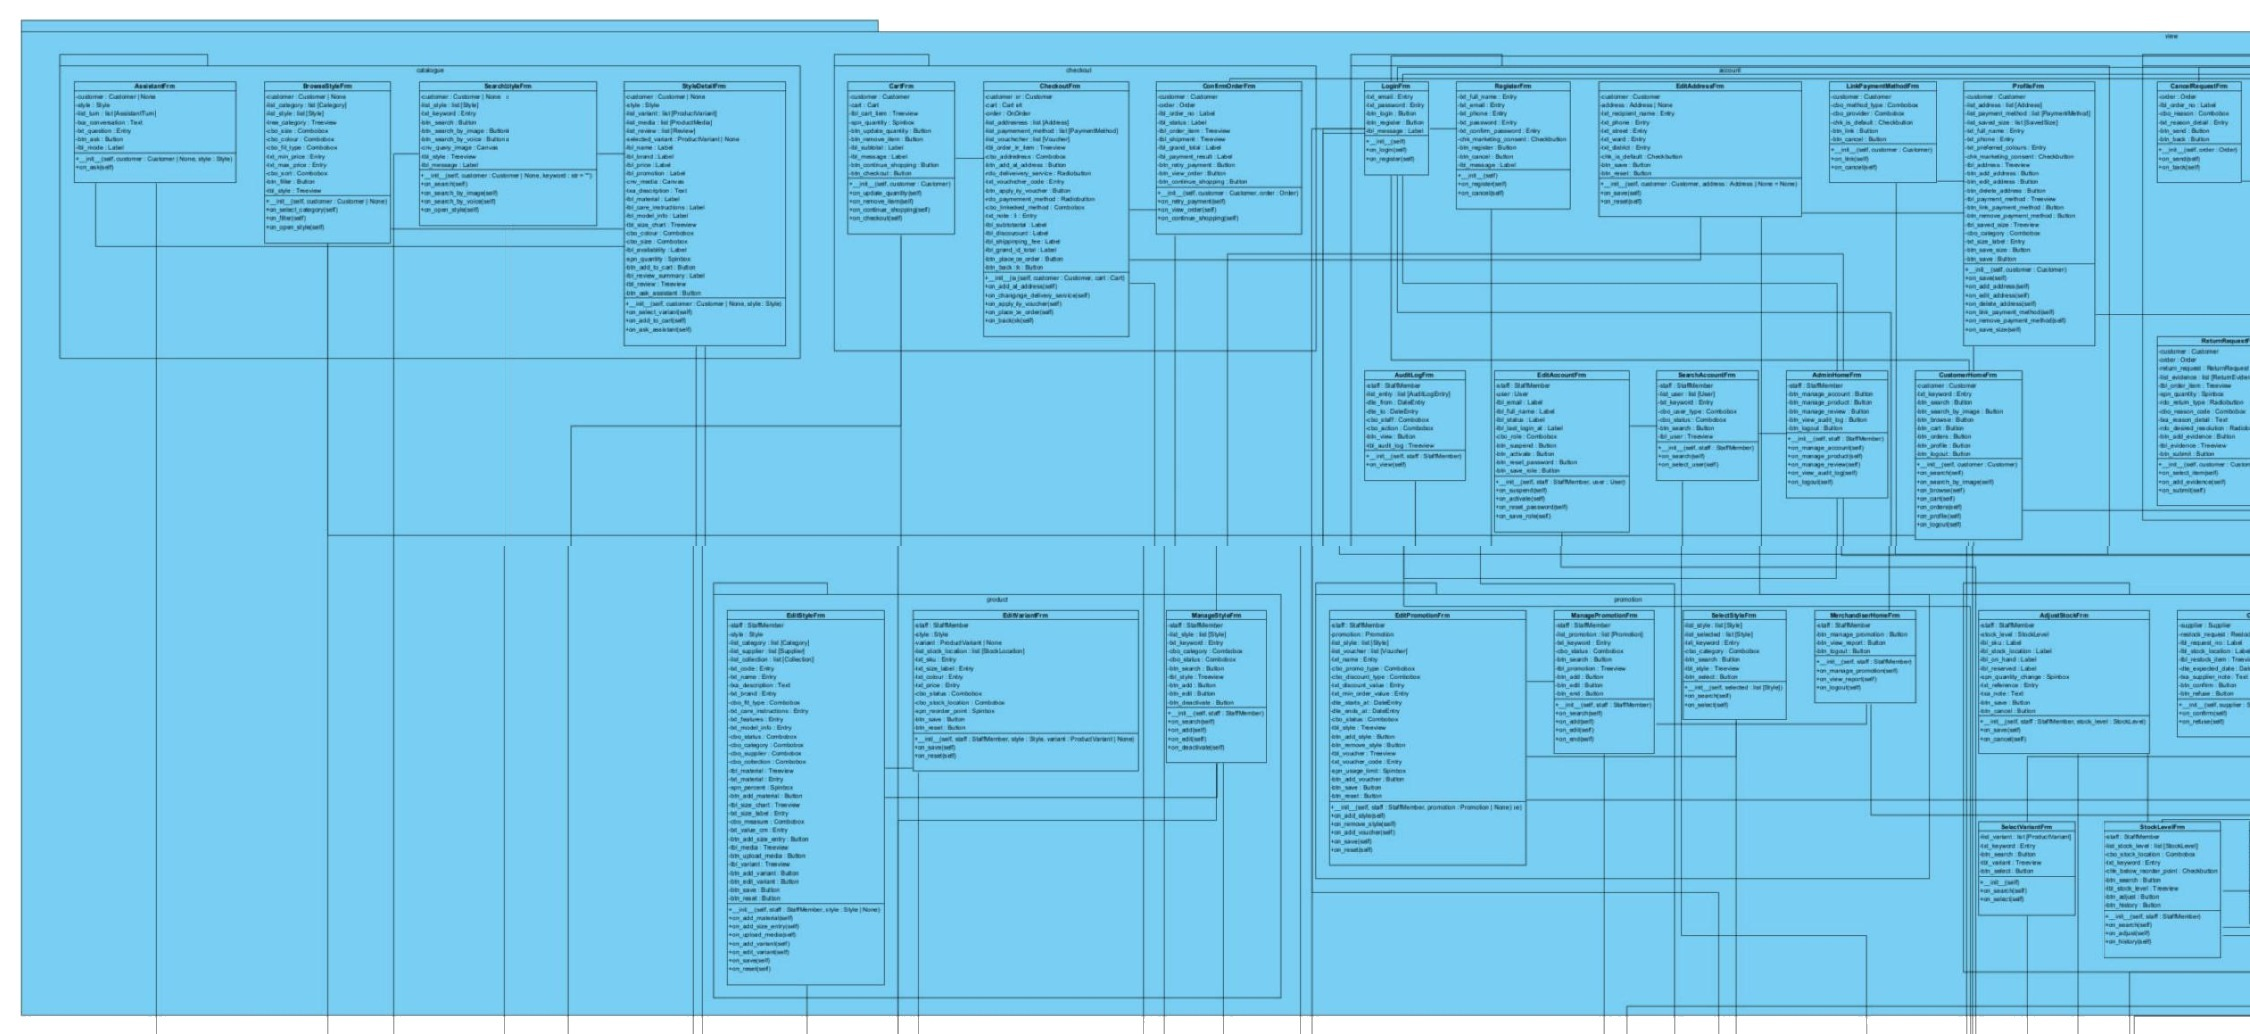
\includegraphics[width=\linewidth,height=0.88\textheight,keepaspectratio]{dc_p1_view_left.jpg}
\caption{Design class diagram, part 1 --- view band, left part --- account, catalogue, checkout and customer-order screens}
\label{fig:design1}
\end{figure}
\end{landscape}

\begin{landscape}
\begin{figure}[p]
\centering
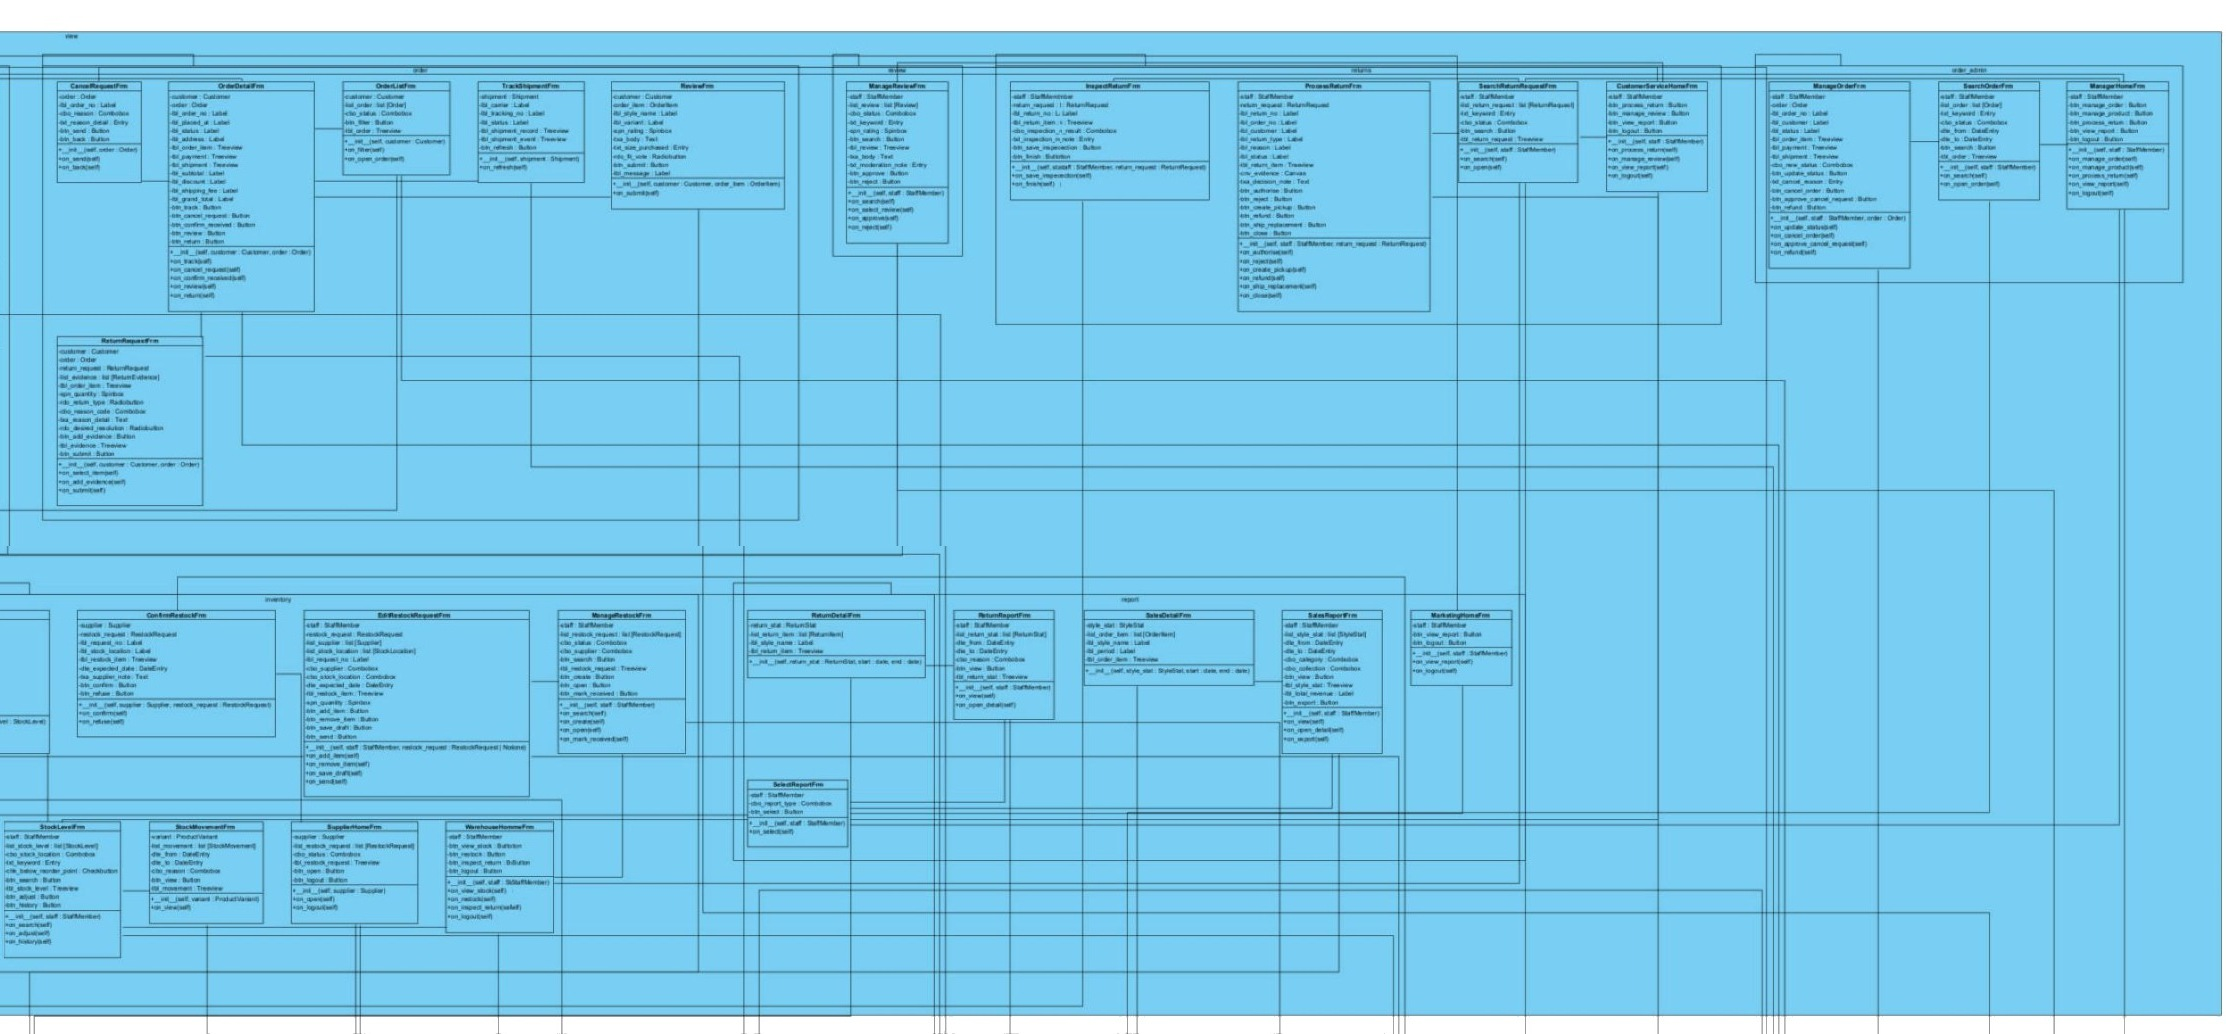
\includegraphics[width=\linewidth,height=0.88\textheight,keepaspectratio]{dc_p2_view_right.jpg}
\caption{Design class diagram, part 2 --- view band, right part --- back-office, inventory, return, review and report screens}
\label{fig:design2}
\end{figure}
\end{landscape}

\begin{landscape}
\begin{figure}[p]
\centering
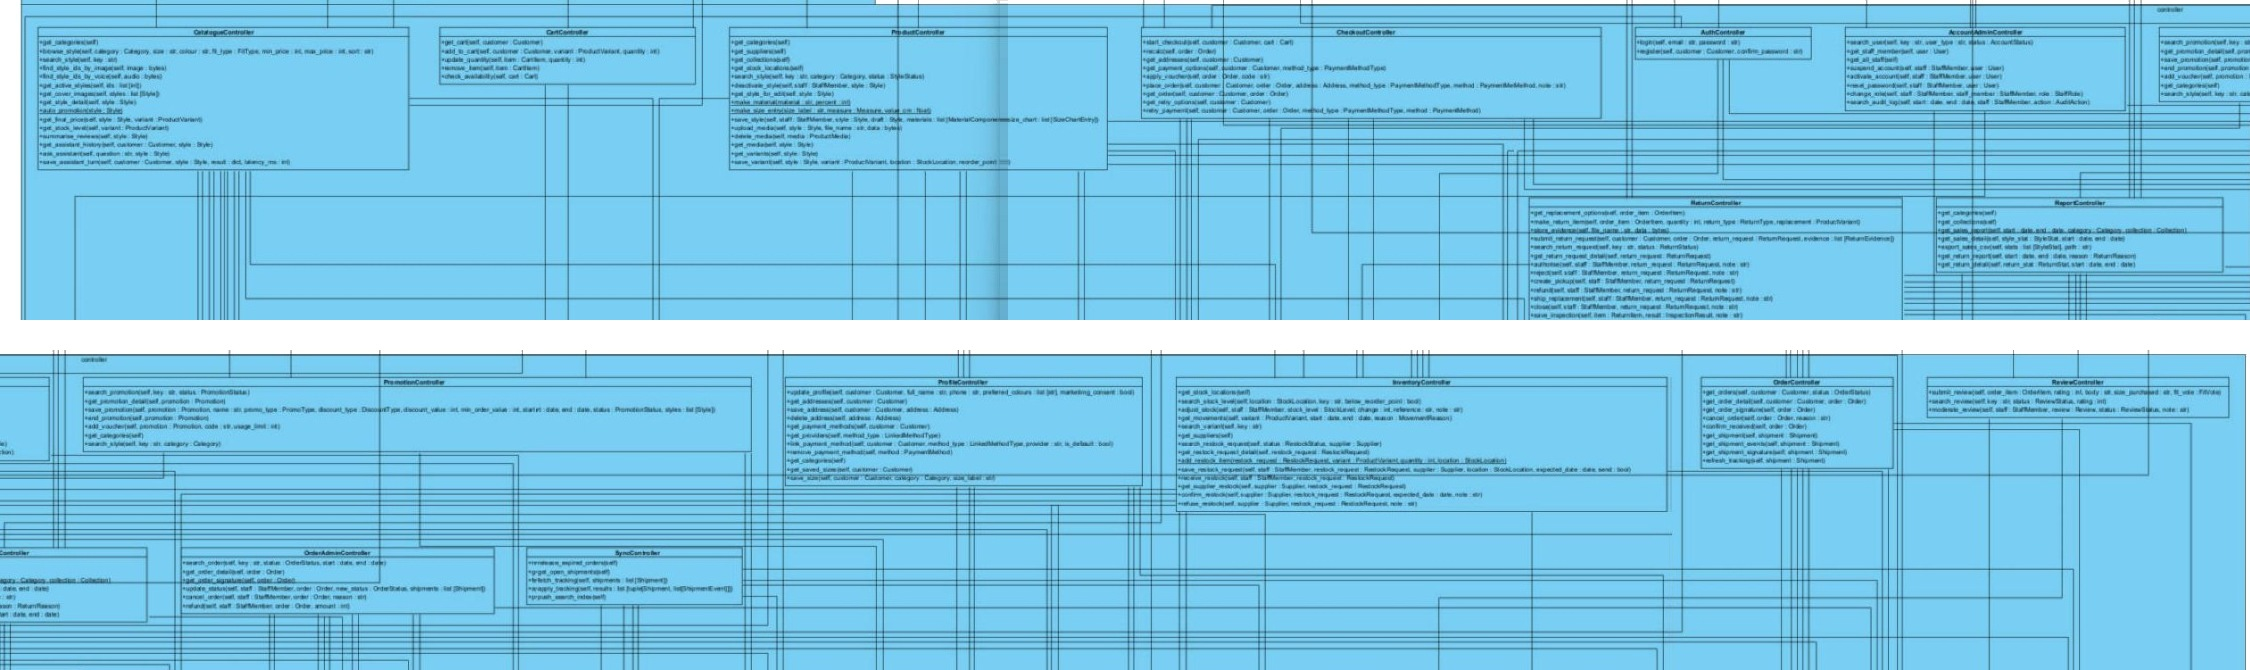
\includegraphics[width=\linewidth,height=0.88\textheight,keepaspectratio]{dc_p3_controller.jpg}
\caption{Design class diagram, part 3 --- controller band --- the 15 controller classes in package \texttt{controller}}
\label{fig:design3}
\end{figure}
\end{landscape}

\begin{landscape}
\begin{figure}[p]
\centering
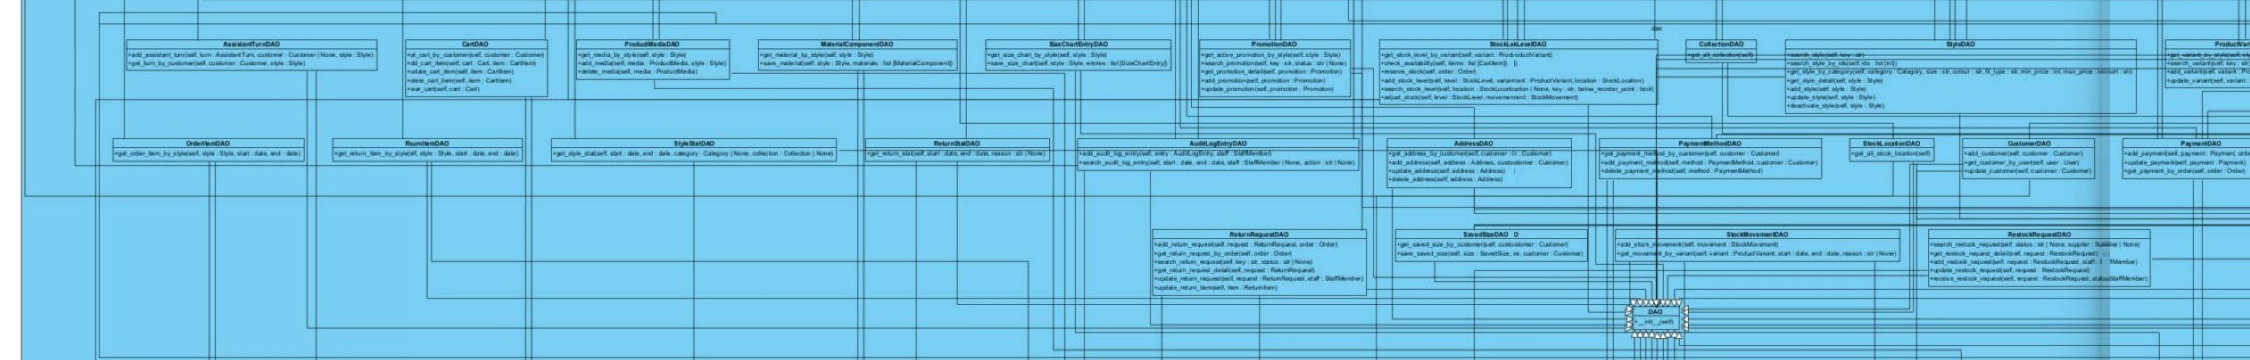
\includegraphics[width=\linewidth,height=0.88\textheight,keepaspectratio]{dc_p4_control_left.jpg}
\caption{Design class diagram, part 4 --- package \texttt{control}, left part --- DAO classes}
\label{fig:design4}
\end{figure}
\end{landscape}

\begin{landscape}
\begin{figure}[p]
\centering
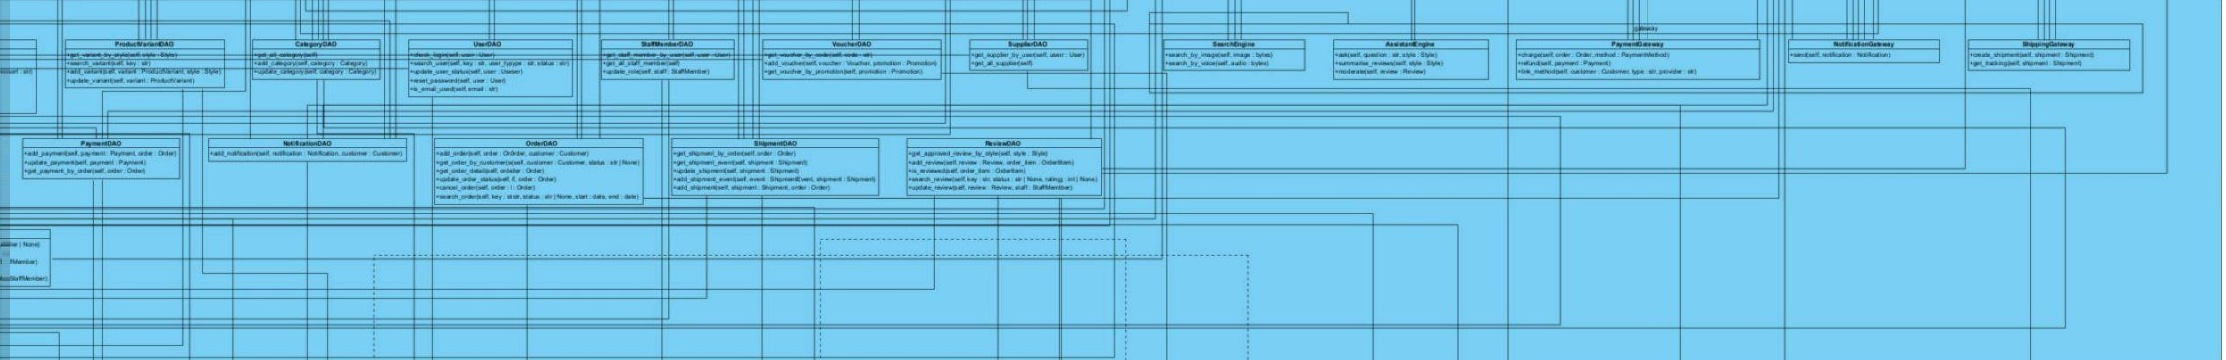
\includegraphics[width=\linewidth,height=0.88\textheight,keepaspectratio]{dc_p5_control_right.jpg}
\caption{Design class diagram, part 5 --- package \texttt{control}, right part --- DAO classes, gateways and the base class \textsf{DAO}}
\label{fig:design5}
\end{figure}
\end{landscape}

\begin{landscape}
\begin{figure}[p]
\centering
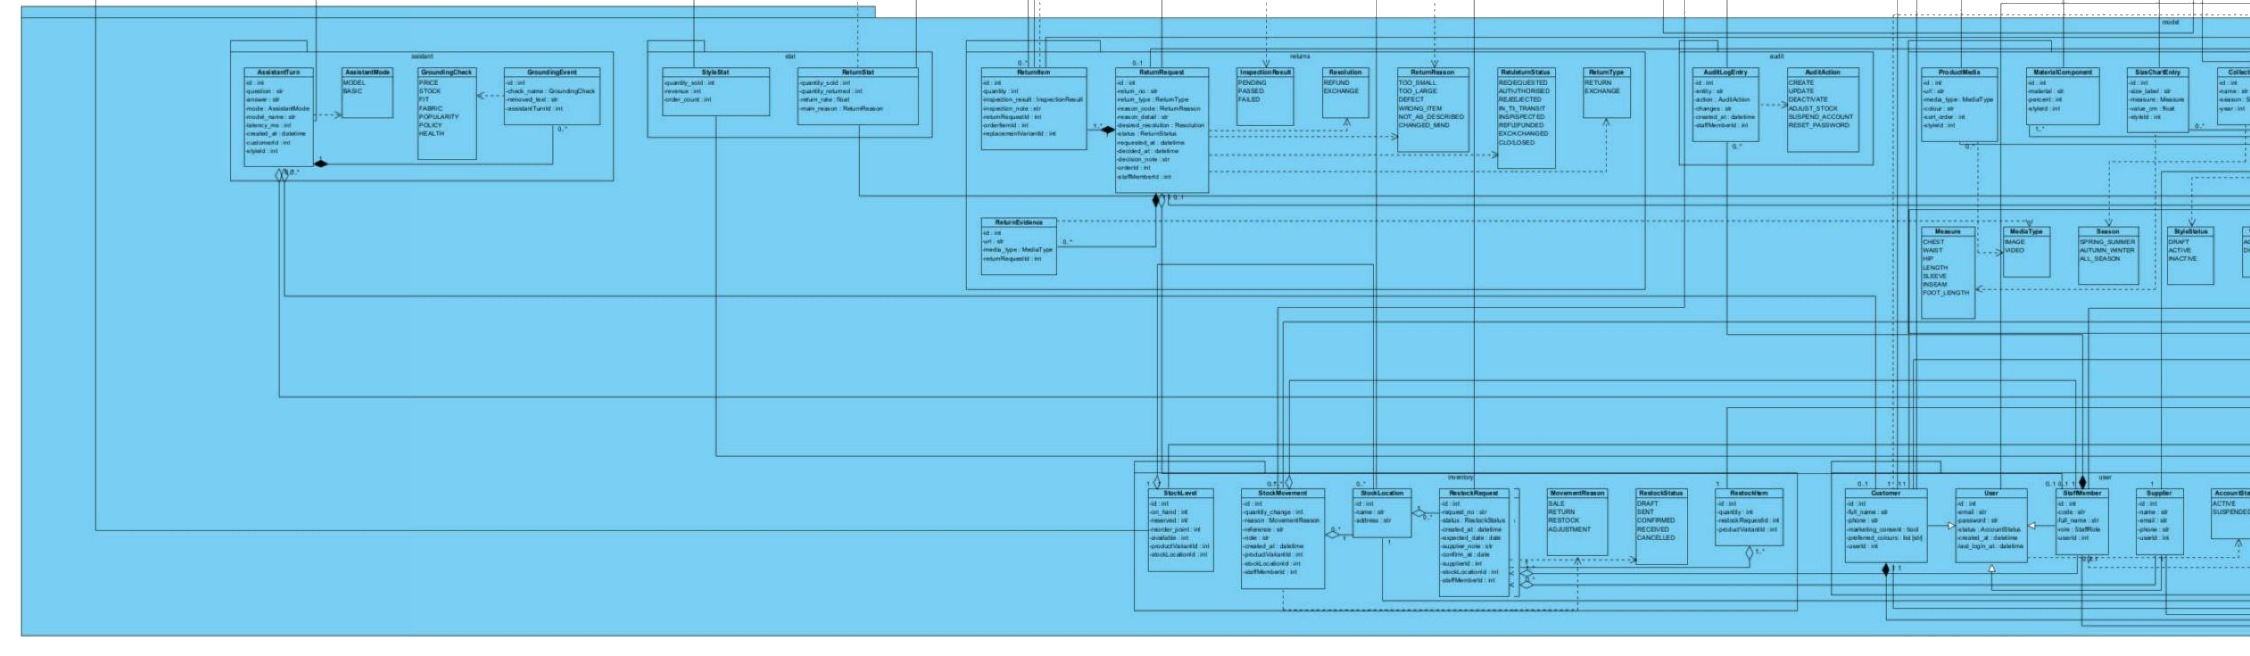
\includegraphics[width=\linewidth,height=0.88\textheight,keepaspectratio]{dc_p6_model_left.jpg}
\caption{Design class diagram, part 6 --- model band, left part --- entity packages with their enumerations}
\label{fig:design6}
\end{figure}
\end{landscape}

\begin{landscape}
\begin{figure}[p]
\centering
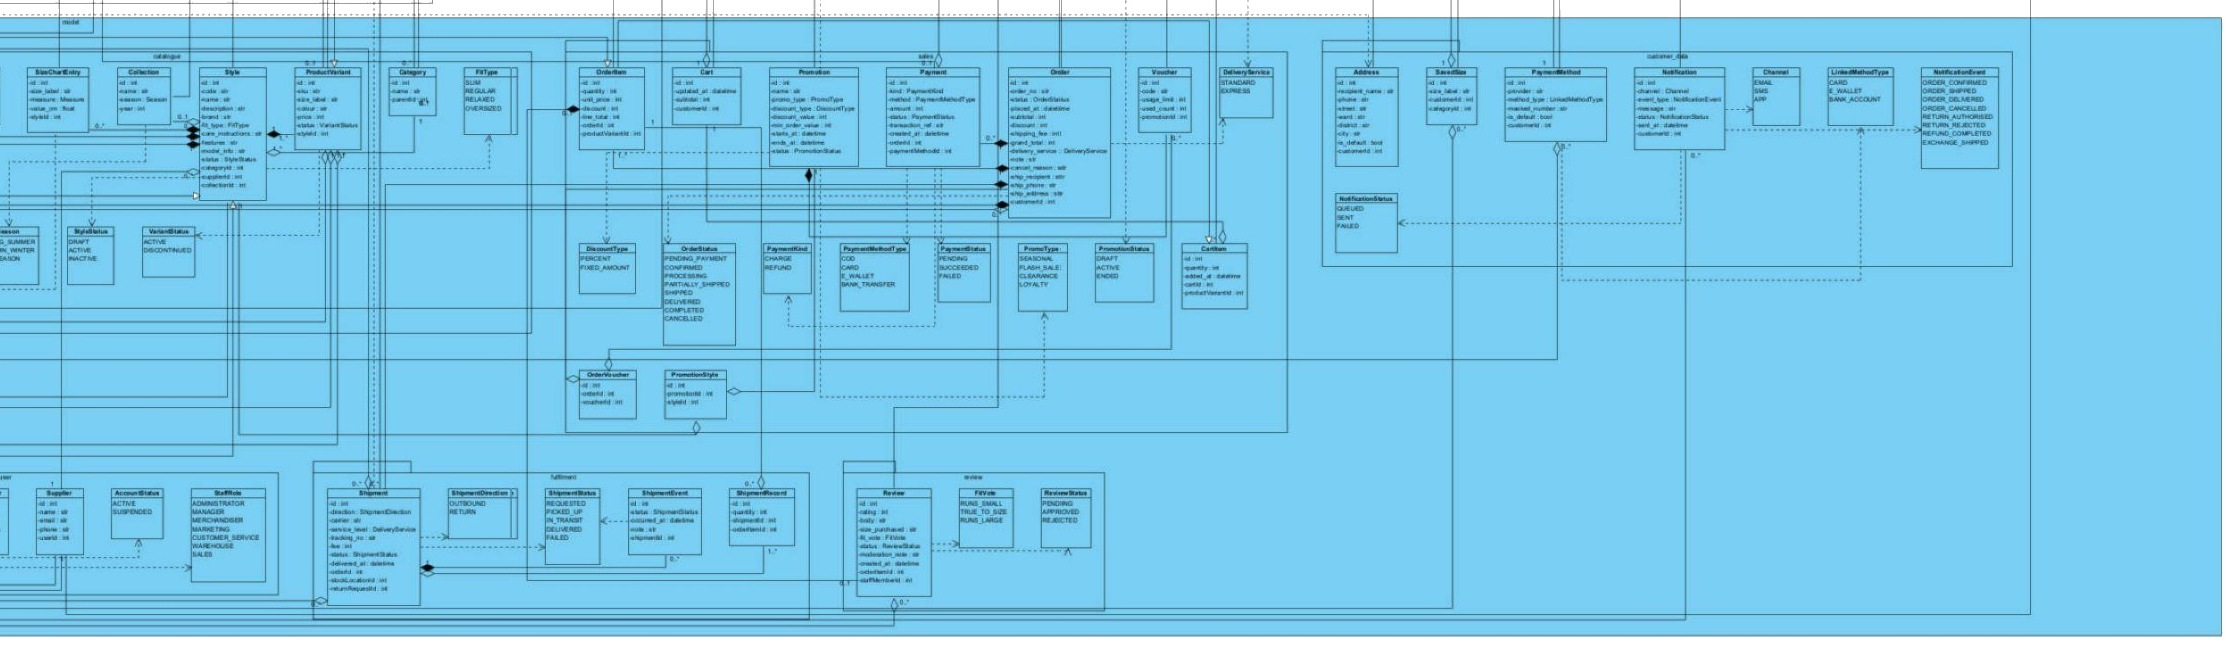
\includegraphics[width=\linewidth,height=0.88\textheight,keepaspectratio]{dc_p7_model_right.jpg}
\caption{Design class diagram, part 7 --- model band, right part --- entity packages with their enumerations}
\label{fig:design7}
\end{figure}
\end{landscape}

\subsection{Entity Classes}
\label{subsec:entityclasses}
The 41 entity classes (Figures~\ref{fig:design6} and~\ref{fig:design7}) are the tables of Section~\ref{subsec:tables} seen from the program: an object of \textsf{Order} is one row of the table \texttt{tblOrder}, and its 15 private attributes are the 15 columns. The class keeps the analysis name; only the table carries the prefix \texttt{tbl}. A DAO creates these objects from the result of a query and turns them back into \texttt{INSERT} and \texttt{UPDATE} statements, so the rest of the program never works with raw rows. Because the attributes and the relationships are the ones already explained in Sections~\ref{sec:analysisclass} and~\ref{sec:datamodel}, they are not repeated here; the design adds only three things:
\begin{itemize}
  \item \textbf{Visibility and types.} All attributes are private and typed: \texttt{-placed\_at: datetime}, \texttt{-grand\_total: int} (Vietnamese dong), \texttt{-status: OrderStatus}. In the code an attribute is read through the object (\texttt{order.status}); its value can only be one of the members of the enumeration.
  \item \textbf{Keys as attributes.} The primary key \texttt{id} and the foreign keys (\texttt{customerId}, \texttt{orderId}, \ldots) are attributes, because a DAO needs them to join and to save the object. The association lines show which object each key points to.
  \item \textbf{Enumerations as classes.} The 34 enumerations (\guillemotleft enumeration\guillemotright) become Python classes \texttt{class OrderStatus(str, Enum)} whose values are exactly the values allowed by the CHECK constraints of the database (Table~\ref{tab:dbrules}).
\end{itemize}

\subsection{View Classes}
\label{subsec:viewclasses}
The 53 view classes are grouped by module in Table~\ref{tab:frmclasses}. For each class the table gives the entity objects it holds, a count of its user-interface components, its operations, the screens it opens and the controller it calls (the associations of Figures~\ref{fig:design1} and~\ref{fig:design2}). Every view calls exactly one controller --- only \textsf{StyleDetailFrm} calls two, \textsf{CatalogueController} and \textsf{CartController} --- and no DAO or gateway; the seven home screens and \textsf{SelectReportFrm} only open other screens and call no controller. Every module starts from a home screen of its actor, which is opened by \textsf{LoginFrm} according to the role of the user.

{\small
\begin{xltabular}{\textwidth}{@{}L{3.9cm} Y L{4.4cm}@{}}
\caption{View (\textsf{Frm}) classes: attributes and operations}\label{tab:frmclasses}\\
\toprule
\textbf{Class} & \textbf{Attributes} & \textbf{Operations} \\ \midrule
\endfirsthead
\toprule
\textbf{Class} & \textbf{Attributes} & \textbf{Operations} \\ \midrule
\endhead
\bottomrule
\endlastfoot
\multicolumn{3}{@{}l}{\emph{Account (UC01--UC03,\allowbreak{} UC20)}} \\
\textbf{LoginFrm} & \textit{Entity objects:} ---. \textit{Widgets:} 2 Entry,\allowbreak{} 2 Button,\allowbreak{} 1 Label. & \texttt{\_\allowbreak{}\_\allowbreak{}init\_\allowbreak{}\_\allowbreak{}(self)},\allowbreak{} \texttt{on\_\allowbreak{}login},\allowbreak{} \texttt{on\_\allowbreak{}register} \\
 & \multicolumn{2}{@{}p{11.9cm}@{}}{\footnotesize Opens: AdminHomeFrm,\allowbreak{} CustomerHomeFrm,\allowbreak{} CustomerServiceHomeFrm,\allowbreak{} ManagerHomeFrm,\allowbreak{} MarketingHomeFrm,\allowbreak{} MerchandiserHomeFrm,\allowbreak{} RegisterFrm,\allowbreak{} SupplierHomeFrm,\allowbreak{} WarehouseHomeFrm. Calls: AuthController.} \\ \addlinespace[2pt]
\textbf{RegisterFrm} & \textit{Entity objects:} ---. \textit{Widgets:} 5 Entry,\allowbreak{} 2 Button,\allowbreak{} 1 Checkbutton,\allowbreak{} 1 Label. & \texttt{\_\allowbreak{}\_\allowbreak{}init\_\allowbreak{}\_\allowbreak{}(self)},\allowbreak{} \texttt{on\_\allowbreak{}register},\allowbreak{} \texttt{on\_\allowbreak{}cancel} \\
 & \multicolumn{2}{@{}p{11.9cm}@{}}{\footnotesize Opens: ---. Calls: AuthController.} \\ \addlinespace[2pt]
\textbf{CustomerHomeFrm} & \textit{Entity objects:} \texttt{customer}: Customer. \textit{Widgets:} 7 Button,\allowbreak{} 1 Entry. & \texttt{\_\allowbreak{}\_\allowbreak{}init\_\allowbreak{}\_\allowbreak{}(self,\allowbreak{} customer)},\allowbreak{} \texttt{on\_\allowbreak{}search},\allowbreak{} \texttt{on\_\allowbreak{}search\_\allowbreak{}by\_\allowbreak{}image},\allowbreak{} \texttt{on\_\allowbreak{}browse},\allowbreak{} \texttt{on\_\allowbreak{}cart},\allowbreak{} \texttt{on\_\allowbreak{}orders},\allowbreak{} \texttt{on\_\allowbreak{}profile},\allowbreak{} \texttt{on\_\allowbreak{}logout} \\
 & \multicolumn{2}{@{}p{11.9cm}@{}}{\footnotesize Opens: BrowseStyleFrm,\allowbreak{} CartFrm,\allowbreak{} OrderListFrm,\allowbreak{} ProfileFrm,\allowbreak{} SearchStyleFrm. Calls: ---.} \\ \addlinespace[2pt]
\textbf{ProfileFrm} & \textit{Entity objects:} \texttt{customer}: Customer,\allowbreak{} \texttt{list\_\allowbreak{}address}: list,\allowbreak{} \texttt{list\_\allowbreak{}payment\_\allowbreak{}method}: list,\allowbreak{} \texttt{list\_\allowbreak{}saved\_\allowbreak{}size}: list. \textit{Widgets:} 7 Button,\allowbreak{} 4 Entry,\allowbreak{} 3 Treeview,\allowbreak{} 1 Checkbutton,\allowbreak{} 1 Combobox. & \texttt{\_\allowbreak{}\_\allowbreak{}init\_\allowbreak{}\_\allowbreak{}(self,\allowbreak{} customer)},\allowbreak{} \texttt{on\_\allowbreak{}save},\allowbreak{} \texttt{on\_\allowbreak{}add\_\allowbreak{}address},\allowbreak{} \texttt{on\_\allowbreak{}edit\_\allowbreak{}address},\allowbreak{} \texttt{on\_\allowbreak{}delete\_\allowbreak{}address},\allowbreak{} \texttt{on\_\allowbreak{}link\_\allowbreak{}payment\_\allowbreak{}method},\allowbreak{} \texttt{on\_\allowbreak{}remove\_\allowbreak{}payment\_\allowbreak{}method},\allowbreak{} \texttt{on\_\allowbreak{}save\_\allowbreak{}size} \\
 & \multicolumn{2}{@{}p{11.9cm}@{}}{\footnotesize Opens: EditAddressFrm,\allowbreak{} LinkPaymentMethodFrm. Calls: ProfileController.} \\ \addlinespace[2pt]
\textbf{EditAddressFrm} & \textit{Entity objects:} \texttt{customer}: Customer,\allowbreak{} \texttt{address}: Address\textbar{}None. \textit{Widgets:} 5 Entry,\allowbreak{} 2 Button,\allowbreak{} 1 Checkbutton. & \texttt{\_\allowbreak{}\_\allowbreak{}init\_\allowbreak{}\_\allowbreak{}(self,\allowbreak{} customer,\allowbreak{} address)},\allowbreak{} \texttt{on\_\allowbreak{}save},\allowbreak{} \texttt{on\_\allowbreak{}reset} \\
 & \multicolumn{2}{@{}p{11.9cm}@{}}{\footnotesize Opens: ---. Calls: ProfileController.} \\ \addlinespace[2pt]
\textbf{LinkPaymentMethodFrm} & \textit{Entity objects:} \texttt{customer}: Customer. \textit{Widgets:} 2 Combobox,\allowbreak{} 2 Button,\allowbreak{} 1 Checkbutton. & \texttt{\_\allowbreak{}\_\allowbreak{}init\_\allowbreak{}\_\allowbreak{}(self,\allowbreak{} customer)},\allowbreak{} \texttt{on\_\allowbreak{}link},\allowbreak{} \texttt{on\_\allowbreak{}cancel} \\
 & \multicolumn{2}{@{}p{11.9cm}@{}}{\footnotesize Opens: ---. Calls: ProfileController.} \\ \addlinespace[2pt]
\textbf{AdminHomeFrm} & \textit{Entity objects:} \texttt{staff}: StaffMember. \textit{Widgets:} 5 Button. & \texttt{\_\allowbreak{}\_\allowbreak{}init\_\allowbreak{}\_\allowbreak{}(self,\allowbreak{} staff)},\allowbreak{} \texttt{on\_\allowbreak{}manage\_\allowbreak{}account},\allowbreak{} \texttt{on\_\allowbreak{}manage\_\allowbreak{}product},\allowbreak{} \texttt{on\_\allowbreak{}manage\_\allowbreak{}review},\allowbreak{} \texttt{on\_\allowbreak{}view\_\allowbreak{}audit\_\allowbreak{}log},\allowbreak{} \texttt{on\_\allowbreak{}logout} \\
 & \multicolumn{2}{@{}p{11.9cm}@{}}{\footnotesize Opens: AuditLogFrm,\allowbreak{} ManageReviewFrm,\allowbreak{} ManageStyleFrm,\allowbreak{} SearchAccountFrm. Calls: ---.} \\ \addlinespace[2pt]
\textbf{SearchAccountFrm} & \textit{Entity objects:} \texttt{staff}: StaffMember,\allowbreak{} \texttt{list\_\allowbreak{}user}: list. \textit{Widgets:} 2 Combobox,\allowbreak{} 1 Entry,\allowbreak{} 1 Button,\allowbreak{} 1 Treeview. & \texttt{\_\allowbreak{}\_\allowbreak{}init\_\allowbreak{}\_\allowbreak{}(self,\allowbreak{} staff)},\allowbreak{} \texttt{on\_\allowbreak{}search},\allowbreak{} \texttt{on\_\allowbreak{}select\_\allowbreak{}user} \\
 & \multicolumn{2}{@{}p{11.9cm}@{}}{\footnotesize Opens: EditAccountFrm. Calls: AccountAdminController.} \\ \addlinespace[2pt]
\textbf{EditAccountFrm} & \textit{Entity objects:} \texttt{staff}: StaffMember,\allowbreak{} \texttt{user}: User. \textit{Widgets:} 4 Label,\allowbreak{} 4 Button,\allowbreak{} 1 Combobox. & \texttt{\_\allowbreak{}\_\allowbreak{}init\_\allowbreak{}\_\allowbreak{}(self,\allowbreak{} staff,\allowbreak{} user)},\allowbreak{} \texttt{on\_\allowbreak{}suspend},\allowbreak{} \texttt{on\_\allowbreak{}activate},\allowbreak{} \texttt{on\_\allowbreak{}reset\_\allowbreak{}password},\allowbreak{} \texttt{on\_\allowbreak{}save\_\allowbreak{}role} \\
 & \multicolumn{2}{@{}p{11.9cm}@{}}{\footnotesize Opens: ---. Calls: AccountAdminController.} \\ \addlinespace[2pt]
\textbf{AuditLogFrm} & \textit{Entity objects:} \texttt{staff}: StaffMember,\allowbreak{} \texttt{list\_\allowbreak{}entry}: list. \textit{Widgets:} 2 DateEntry,\allowbreak{} 2 Combobox,\allowbreak{} 1 Button,\allowbreak{} 1 Treeview. & \texttt{\_\allowbreak{}\_\allowbreak{}init\_\allowbreak{}\_\allowbreak{}(self,\allowbreak{} staff)},\allowbreak{} \texttt{on\_\allowbreak{}view} \\
 & \multicolumn{2}{@{}p{11.9cm}@{}}{\footnotesize Opens: ---. Calls: AccountAdminController.} \\ \addlinespace[2pt]
\multicolumn{3}{@{}l}{\emph{Catalogue and assistant (UC04--UC06,\allowbreak{} UC32,\allowbreak{} UC33)}} \\
\textbf{BrowseStyleFrm} & \textit{Entity objects:} \texttt{customer}: Customer\textbar{}None,\allowbreak{} \texttt{list\_\allowbreak{}category}: list,\allowbreak{} \texttt{list\_\allowbreak{}style}: list. \textit{Widgets:} 4 Combobox,\allowbreak{} 2 Treeview,\allowbreak{} 2 Entry,\allowbreak{} 1 Button. & \texttt{\_\allowbreak{}\_\allowbreak{}init\_\allowbreak{}\_\allowbreak{}(self,\allowbreak{} customer)},\allowbreak{} \texttt{on\_\allowbreak{}select\_\allowbreak{}category},\allowbreak{} \texttt{on\_\allowbreak{}filter},\allowbreak{} \texttt{on\_\allowbreak{}open\_\allowbreak{}style} \\
 & \multicolumn{2}{@{}p{11.9cm}@{}}{\footnotesize Opens: StyleDetailFrm. Calls: CatalogueController.} \\ \addlinespace[2pt]
\textbf{SearchStyleFrm} & \textit{Entity objects:} \texttt{customer}: Customer\textbar{}None,\allowbreak{} \texttt{list\_\allowbreak{}style}: list. \textit{Widgets:} 3 Button,\allowbreak{} 1 Entry,\allowbreak{} 1 Canvas,\allowbreak{} 1 Treeview,\allowbreak{} 1 Label. & \texttt{\_\allowbreak{}\_\allowbreak{}init\_\allowbreak{}\_\allowbreak{}(self,\allowbreak{} customer,\allowbreak{} keyword)},\allowbreak{} \texttt{on\_\allowbreak{}search},\allowbreak{} \texttt{on\_\allowbreak{}search\_\allowbreak{}by\_\allowbreak{}image},\allowbreak{} \texttt{on\_\allowbreak{}search\_\allowbreak{}by\_\allowbreak{}voice},\allowbreak{} \texttt{on\_\allowbreak{}open\_\allowbreak{}style} \\
 & \multicolumn{2}{@{}p{11.9cm}@{}}{\footnotesize Opens: StyleDetailFrm. Calls: CatalogueController.} \\ \addlinespace[2pt]
\textbf{StyleDetailFrm} & \textit{Entity objects:} \texttt{customer}: Customer\textbar{}None,\allowbreak{} \texttt{style}: Style,\allowbreak{} \texttt{list\_\allowbreak{}variant}: list,\allowbreak{} \texttt{list\_\allowbreak{}media}: list,\allowbreak{} \texttt{list\_\allowbreak{}review}: list,\allowbreak{} \texttt{selected\_\allowbreak{}variant}: ProductVariant\textbar{}None. \textit{Widgets:} 9 Label,\allowbreak{} 2 Treeview,\allowbreak{} 2 Combobox,\allowbreak{} 2 Button,\allowbreak{} 1 Canvas,\allowbreak{} 1 Text,\allowbreak{} 1 Spinbox. & \texttt{\_\allowbreak{}\_\allowbreak{}init\_\allowbreak{}\_\allowbreak{}(self,\allowbreak{} customer,\allowbreak{} style)},\allowbreak{} \texttt{on\_\allowbreak{}select\_\allowbreak{}variant},\allowbreak{} \texttt{on\_\allowbreak{}add\_\allowbreak{}to\_\allowbreak{}cart},\allowbreak{} \texttt{on\_\allowbreak{}ask\_\allowbreak{}assistant} \\
 & \multicolumn{2}{@{}p{11.9cm}@{}}{\footnotesize Opens: AssistantFrm. Calls: CartController,\allowbreak{} CatalogueController.} \\ \addlinespace[2pt]
\textbf{AssistantFrm} & \textit{Entity objects:} \texttt{customer}: Customer\textbar{}None,\allowbreak{} \texttt{style}: Style,\allowbreak{} \texttt{list\_\allowbreak{}turn}: list. \textit{Widgets:} 1 Text,\allowbreak{} 1 Entry,\allowbreak{} 1 Button,\allowbreak{} 1 Label. & \texttt{\_\allowbreak{}\_\allowbreak{}init\_\allowbreak{}\_\allowbreak{}(self,\allowbreak{} customer,\allowbreak{} style)},\allowbreak{} \texttt{on\_\allowbreak{}ask} \\
 & \multicolumn{2}{@{}p{11.9cm}@{}}{\footnotesize Opens: ---. Calls: CatalogueController.} \\ \addlinespace[2pt]
\multicolumn{3}{@{}l}{\emph{Cart and checkout (UC07,\allowbreak{} UC08,\allowbreak{} UC25,\allowbreak{} UC26,\allowbreak{} UC28--UC31)}} \\
\textbf{CartFrm} & \textit{Entity objects:} \texttt{customer}: Customer,\allowbreak{} \texttt{cart}: Cart. \textit{Widgets:} 4 Button,\allowbreak{} 2 Label,\allowbreak{} 1 Treeview,\allowbreak{} 1 Spinbox. & \texttt{\_\allowbreak{}\_\allowbreak{}init\_\allowbreak{}\_\allowbreak{}(self,\allowbreak{} customer)},\allowbreak{} \texttt{on\_\allowbreak{}update\_\allowbreak{}quantity},\allowbreak{} \texttt{on\_\allowbreak{}remove\_\allowbreak{}item},\allowbreak{} \texttt{on\_\allowbreak{}continue\_\allowbreak{}shopping},\allowbreak{} \texttt{on\_\allowbreak{}checkout} \\
 & \multicolumn{2}{@{}p{11.9cm}@{}}{\footnotesize Opens: CheckoutFrm. Calls: CartController.} \\ \addlinespace[2pt]
\textbf{CheckoutFrm} & \textit{Entity objects:} \texttt{customer}: Customer,\allowbreak{} \texttt{cart}: Cart,\allowbreak{} \texttt{order}: Order,\allowbreak{} \texttt{list\_\allowbreak{}address}: list,\allowbreak{} \texttt{list\_\allowbreak{}payment\_\allowbreak{}method}: list,\allowbreak{} \texttt{list\_\allowbreak{}voucher}: list. \textit{Widgets:} 4 Button,\allowbreak{} 4 Label,\allowbreak{} 2 Combobox,\allowbreak{} 2 Radiobutton,\allowbreak{} 2 Entry,\allowbreak{} 1 Treeview. & \texttt{\_\allowbreak{}\_\allowbreak{}init\_\allowbreak{}\_\allowbreak{}(self,\allowbreak{} customer,\allowbreak{} cart)},\allowbreak{} \texttt{on\_\allowbreak{}add\_\allowbreak{}address},\allowbreak{} \texttt{on\_\allowbreak{}change\_\allowbreak{}delivery\_\allowbreak{}service},\allowbreak{} \texttt{on\_\allowbreak{}apply\_\allowbreak{}voucher},\allowbreak{} \texttt{on\_\allowbreak{}place\_\allowbreak{}order},\allowbreak{} \texttt{on\_\allowbreak{}back} \\
 & \multicolumn{2}{@{}p{11.9cm}@{}}{\footnotesize Opens: ConfirmOrderFrm,\allowbreak{} EditAddressFrm. Calls: CheckoutController.} \\ \addlinespace[2pt]
\textbf{ConfirmOrderFrm} & \textit{Entity objects:} \texttt{customer}: Customer,\allowbreak{} \texttt{order}: Order. \textit{Widgets:} 4 Label,\allowbreak{} 3 Button,\allowbreak{} 2 Treeview. & \texttt{\_\allowbreak{}\_\allowbreak{}init\_\allowbreak{}\_\allowbreak{}(self,\allowbreak{} customer,\allowbreak{} order)},\allowbreak{} \texttt{on\_\allowbreak{}retry\_\allowbreak{}payment},\allowbreak{} \texttt{on\_\allowbreak{}view\_\allowbreak{}order},\allowbreak{} \texttt{on\_\allowbreak{}continue\_\allowbreak{}shopping} \\
 & \multicolumn{2}{@{}p{11.9cm}@{}}{\footnotesize Opens: OrderDetailFrm. Calls: CheckoutController.} \\ \addlinespace[2pt]
\multicolumn{3}{@{}l}{\emph{Customer orders (UC09--UC14,\allowbreak{} UC34)}} \\
\textbf{OrderListFrm} & \textit{Entity objects:} \texttt{customer}: Customer,\allowbreak{} \texttt{list\_\allowbreak{}order}: list. \textit{Widgets:} 1 Combobox,\allowbreak{} 1 Button,\allowbreak{} 1 Treeview. & \texttt{\_\allowbreak{}\_\allowbreak{}init\_\allowbreak{}\_\allowbreak{}(self,\allowbreak{} customer)},\allowbreak{} \texttt{on\_\allowbreak{}filter},\allowbreak{} \texttt{on\_\allowbreak{}open\_\allowbreak{}order} \\
 & \multicolumn{2}{@{}p{11.9cm}@{}}{\footnotesize Opens: OrderDetailFrm. Calls: OrderController.} \\ \addlinespace[2pt]
\textbf{OrderDetailFrm} & \textit{Entity objects:} \texttt{customer}: Customer,\allowbreak{} \texttt{order}: Order. \textit{Widgets:} 8 Label,\allowbreak{} 5 Button,\allowbreak{} 3 Treeview. & \texttt{\_\allowbreak{}\_\allowbreak{}init\_\allowbreak{}\_\allowbreak{}(self,\allowbreak{} customer,\allowbreak{} order)},\allowbreak{} \texttt{on\_\allowbreak{}track},\allowbreak{} \texttt{on\_\allowbreak{}cancel\_\allowbreak{}request},\allowbreak{} \texttt{on\_\allowbreak{}confirm\_\allowbreak{}received},\allowbreak{} \texttt{on\_\allowbreak{}review},\allowbreak{} \texttt{on\_\allowbreak{}return} \\
 & \multicolumn{2}{@{}p{11.9cm}@{}}{\footnotesize Opens: CancelRequestFrm,\allowbreak{} ReturnRequestFrm,\allowbreak{} ReviewFrm,\allowbreak{} TrackShipmentFrm. Calls: OrderController.} \\ \addlinespace[2pt]
\textbf{TrackShipmentFrm} & \textit{Entity objects:} \texttt{shipment}: Shipment. \textit{Widgets:} 3 Label,\allowbreak{} 2 Treeview,\allowbreak{} 1 Button. & \texttt{\_\allowbreak{}\_\allowbreak{}init\_\allowbreak{}\_\allowbreak{}(self,\allowbreak{} shipment)},\allowbreak{} \texttt{on\_\allowbreak{}refresh} \\
 & \multicolumn{2}{@{}p{11.9cm}@{}}{\footnotesize Opens: ---. Calls: OrderController.} \\ \addlinespace[2pt]
\textbf{CancelRequestFrm} & \textit{Entity objects:} \texttt{order}: Order. \textit{Widgets:} 2 Button,\allowbreak{} 1 Label,\allowbreak{} 1 Combobox,\allowbreak{} 1 Entry. & \texttt{\_\allowbreak{}\_\allowbreak{}init\_\allowbreak{}\_\allowbreak{}(self,\allowbreak{} order)},\allowbreak{} \texttt{on\_\allowbreak{}send},\allowbreak{} \texttt{on\_\allowbreak{}back} \\
 & \multicolumn{2}{@{}p{11.9cm}@{}}{\footnotesize Opens: ---. Calls: OrderController.} \\ \addlinespace[2pt]
\textbf{ReviewFrm} & \textit{Entity objects:} \texttt{customer}: Customer,\allowbreak{} \texttt{order\_\allowbreak{}item}: OrderItem. \textit{Widgets:} 3 Label,\allowbreak{} 1 Spinbox,\allowbreak{} 1 Text,\allowbreak{} 1 Entry,\allowbreak{} 1 Radiobutton,\allowbreak{} 1 Button. & \texttt{\_\allowbreak{}\_\allowbreak{}init\_\allowbreak{}\_\allowbreak{}(self,\allowbreak{} customer,\allowbreak{} order\_\allowbreak{}item)},\allowbreak{} \texttt{on\_\allowbreak{}submit} \\
 & \multicolumn{2}{@{}p{11.9cm}@{}}{\footnotesize Opens: ---. Calls: ReviewController.} \\ \addlinespace[2pt]
\textbf{ReturnRequestFrm} & \textit{Entity objects:} \texttt{customer}: Customer,\allowbreak{} \texttt{order}: Order,\allowbreak{} \texttt{return\_\allowbreak{}request}: ReturnRequest,\allowbreak{} \texttt{list\_\allowbreak{}evidence}: list. \textit{Widgets:} 2 Treeview,\allowbreak{} 2 Radiobutton,\allowbreak{} 2 Button,\allowbreak{} 1 Spinbox,\allowbreak{} 1 Combobox,\allowbreak{} 1 Text. & \texttt{\_\allowbreak{}\_\allowbreak{}init\_\allowbreak{}\_\allowbreak{}(self,\allowbreak{} customer,\allowbreak{} order)},\allowbreak{} \texttt{on\_\allowbreak{}select\_\allowbreak{}item},\allowbreak{} \texttt{on\_\allowbreak{}add\_\allowbreak{}evidence},\allowbreak{} \texttt{on\_\allowbreak{}submit} \\
 & \multicolumn{2}{@{}p{11.9cm}@{}}{\footnotesize Opens: ---. Calls: ReturnController.} \\ \addlinespace[2pt]
\multicolumn{3}{@{}l}{\emph{Order management (UC22,\allowbreak{} UC23)}} \\
\textbf{ManagerHomeFrm} & \textit{Entity objects:} \texttt{staff}: StaffMember. \textit{Widgets:} 5 Button. & \texttt{\_\allowbreak{}\_\allowbreak{}init\_\allowbreak{}\_\allowbreak{}(self,\allowbreak{} staff)},\allowbreak{} \texttt{on\_\allowbreak{}manage\_\allowbreak{}order},\allowbreak{} \texttt{on\_\allowbreak{}manage\_\allowbreak{}product},\allowbreak{} \texttt{on\_\allowbreak{}process\_\allowbreak{}return},\allowbreak{} \texttt{on\_\allowbreak{}view\_\allowbreak{}report},\allowbreak{} \texttt{on\_\allowbreak{}logout} \\
 & \multicolumn{2}{@{}p{11.9cm}@{}}{\footnotesize Opens: ManageStyleFrm,\allowbreak{} SearchOrderFrm,\allowbreak{} SearchReturnRequestFrm,\allowbreak{} SelectReportFrm. Calls: ---.} \\ \addlinespace[2pt]
\textbf{SearchOrderFrm} & \textit{Entity objects:} \texttt{staff}: StaffMember,\allowbreak{} \texttt{list\_\allowbreak{}order}: list. \textit{Widgets:} 2 DateEntry,\allowbreak{} 1 Entry,\allowbreak{} 1 Combobox,\allowbreak{} 1 Button,\allowbreak{} 1 Treeview. & \texttt{\_\allowbreak{}\_\allowbreak{}init\_\allowbreak{}\_\allowbreak{}(self,\allowbreak{} staff)},\allowbreak{} \texttt{on\_\allowbreak{}search},\allowbreak{} \texttt{on\_\allowbreak{}open\_\allowbreak{}order} \\
 & \multicolumn{2}{@{}p{11.9cm}@{}}{\footnotesize Opens: ManageOrderFrm. Calls: OrderAdminController.} \\ \addlinespace[2pt]
\textbf{ManageOrderFrm} & \textit{Entity objects:} \texttt{staff}: StaffMember,\allowbreak{} \texttt{order}: Order. \textit{Widgets:} 4 Button,\allowbreak{} 3 Label,\allowbreak{} 3 Treeview,\allowbreak{} 1 Combobox,\allowbreak{} 1 Entry. & \texttt{\_\allowbreak{}\_\allowbreak{}init\_\allowbreak{}\_\allowbreak{}(self,\allowbreak{} staff,\allowbreak{} order)},\allowbreak{} \texttt{on\_\allowbreak{}update\_\allowbreak{}status},\allowbreak{} \texttt{on\_\allowbreak{}cancel\_\allowbreak{}order},\allowbreak{} \texttt{on\_\allowbreak{}approve\_\allowbreak{}cancel\_\allowbreak{}request},\allowbreak{} \texttt{on\_\allowbreak{}refund} \\
 & \multicolumn{2}{@{}p{11.9cm}@{}}{\footnotesize Opens: ---. Calls: OrderAdminController.} \\ \addlinespace[2pt]
\multicolumn{3}{@{}l}{\emph{Product management (UC21)}} \\
\textbf{ManageStyleFrm} & \textit{Entity objects:} \texttt{staff}: StaffMember,\allowbreak{} \texttt{list\_\allowbreak{}style}: list. \textit{Widgets:} 4 Button,\allowbreak{} 2 Combobox,\allowbreak{} 1 Entry,\allowbreak{} 1 Treeview. & \texttt{\_\allowbreak{}\_\allowbreak{}init\_\allowbreak{}\_\allowbreak{}(self,\allowbreak{} staff)},\allowbreak{} \texttt{on\_\allowbreak{}search},\allowbreak{} \texttt{on\_\allowbreak{}add},\allowbreak{} \texttt{on\_\allowbreak{}edit},\allowbreak{} \texttt{on\_\allowbreak{}deactivate} \\
 & \multicolumn{2}{@{}p{11.9cm}@{}}{\footnotesize Opens: EditStyleFrm. Calls: ProductController.} \\ \addlinespace[2pt]
\textbf{EditStyleFrm} & \textit{Entity objects:} \texttt{staff}: StaffMember,\allowbreak{} \texttt{style}: Style,\allowbreak{} \texttt{list\_\allowbreak{}category}: list,\allowbreak{} \texttt{list\_\allowbreak{}supplier}: list,\allowbreak{} \texttt{list\_\allowbreak{}collection}: list. \textit{Widgets:} 9 Entry,\allowbreak{} 7 Button,\allowbreak{} 6 Combobox,\allowbreak{} 4 Treeview,\allowbreak{} 1 Text,\allowbreak{} 1 Spinbox. & \texttt{\_\allowbreak{}\_\allowbreak{}init\_\allowbreak{}\_\allowbreak{}(self,\allowbreak{} staff,\allowbreak{} style)},\allowbreak{} \texttt{on\_\allowbreak{}add\_\allowbreak{}material},\allowbreak{} \texttt{on\_\allowbreak{}add\_\allowbreak{}size\_\allowbreak{}entry},\allowbreak{} \texttt{on\_\allowbreak{}upload\_\allowbreak{}media},\allowbreak{} \texttt{on\_\allowbreak{}add\_\allowbreak{}variant},\allowbreak{} \texttt{on\_\allowbreak{}edit\_\allowbreak{}variant},\allowbreak{} \texttt{on\_\allowbreak{}save},\allowbreak{} \texttt{on\_\allowbreak{}reset} \\
 & \multicolumn{2}{@{}p{11.9cm}@{}}{\footnotesize Opens: EditVariantFrm. Calls: ProductController.} \\ \addlinespace[2pt]
\textbf{EditVariantFrm} & \textit{Entity objects:} \texttt{staff}: StaffMember,\allowbreak{} \texttt{style}: Style,\allowbreak{} \texttt{variant}: ProductVariant\textbar{}None,\allowbreak{} \texttt{list\_\allowbreak{}stock\_\allowbreak{}location}: list. \textit{Widgets:} 4 Entry,\allowbreak{} 2 Combobox,\allowbreak{} 2 Button,\allowbreak{} 1 Spinbox. & \texttt{\_\allowbreak{}\_\allowbreak{}init\_\allowbreak{}\_\allowbreak{}(self,\allowbreak{} staff,\allowbreak{} style,\allowbreak{} variant)},\allowbreak{} \texttt{on\_\allowbreak{}save},\allowbreak{} \texttt{on\_\allowbreak{}reset} \\
 & \multicolumn{2}{@{}p{11.9cm}@{}}{\footnotesize Opens: ---. Calls: ProductController.} \\ \addlinespace[2pt]
\multicolumn{3}{@{}l}{\emph{Promotions (UC15,\allowbreak{} UC27)}} \\
\textbf{MerchandiserHomeFrm} & \textit{Entity objects:} \texttt{staff}: StaffMember. \textit{Widgets:} 3 Button. & \texttt{\_\allowbreak{}\_\allowbreak{}init\_\allowbreak{}\_\allowbreak{}(self,\allowbreak{} staff)},\allowbreak{} \texttt{on\_\allowbreak{}manage\_\allowbreak{}promotion},\allowbreak{} \texttt{on\_\allowbreak{}view\_\allowbreak{}report},\allowbreak{} \texttt{on\_\allowbreak{}logout} \\
 & \multicolumn{2}{@{}p{11.9cm}@{}}{\footnotesize Opens: ManagePromotionFrm,\allowbreak{} SelectReportFrm. Calls: ---.} \\ \addlinespace[2pt]
\textbf{ManagePromotionFrm} & \textit{Entity objects:} \texttt{staff}: StaffMember,\allowbreak{} \texttt{list\_\allowbreak{}promotion}: list. \textit{Widgets:} 4 Button,\allowbreak{} 1 Entry,\allowbreak{} 1 Combobox,\allowbreak{} 1 Treeview. & \texttt{\_\allowbreak{}\_\allowbreak{}init\_\allowbreak{}\_\allowbreak{}(self,\allowbreak{} staff)},\allowbreak{} \texttt{on\_\allowbreak{}search},\allowbreak{} \texttt{on\_\allowbreak{}add},\allowbreak{} \texttt{on\_\allowbreak{}edit},\allowbreak{} \texttt{on\_\allowbreak{}end} \\
 & \multicolumn{2}{@{}p{11.9cm}@{}}{\footnotesize Opens: EditPromotionFrm. Calls: PromotionController.} \\ \addlinespace[2pt]
\textbf{EditPromotionFrm} & \textit{Entity objects:} \texttt{staff}: StaffMember,\allowbreak{} \texttt{promotion}: Promotion,\allowbreak{} \texttt{list\_\allowbreak{}style}: list,\allowbreak{} \texttt{list\_\allowbreak{}voucher}: list. \textit{Widgets:} 5 Button,\allowbreak{} 4 Entry,\allowbreak{} 3 Combobox,\allowbreak{} 2 DateEntry,\allowbreak{} 2 Treeview,\allowbreak{} 1 Spinbox. & \texttt{\_\allowbreak{}\_\allowbreak{}init\_\allowbreak{}\_\allowbreak{}(self,\allowbreak{} staff,\allowbreak{} promotion)},\allowbreak{} \texttt{on\_\allowbreak{}add\_\allowbreak{}style},\allowbreak{} \texttt{on\_\allowbreak{}remove\_\allowbreak{}style},\allowbreak{} \texttt{on\_\allowbreak{}add\_\allowbreak{}voucher},\allowbreak{} \texttt{on\_\allowbreak{}save},\allowbreak{} \texttt{on\_\allowbreak{}reset} \\
 & \multicolumn{2}{@{}p{11.9cm}@{}}{\footnotesize Opens: SelectStyleFrm. Calls: PromotionController.} \\ \addlinespace[2pt]
\textbf{SelectStyleFrm} & \textit{Entity objects:} \texttt{list\_\allowbreak{}style}: list,\allowbreak{} \texttt{list\_\allowbreak{}selected}: list. \textit{Widgets:} 2 Button,\allowbreak{} 1 Entry,\allowbreak{} 1 Combobox,\allowbreak{} 1 Treeview. & \texttt{\_\allowbreak{}\_\allowbreak{}init\_\allowbreak{}\_\allowbreak{}(self,\allowbreak{} selected)},\allowbreak{} \texttt{on\_\allowbreak{}search},\allowbreak{} \texttt{on\_\allowbreak{}select} \\
 & \multicolumn{2}{@{}p{11.9cm}@{}}{\footnotesize Opens: ---. Calls: PromotionController.} \\ \addlinespace[2pt]
\multicolumn{3}{@{}l}{\emph{Inventory and restocking (UC17)}} \\
\textbf{WarehouseHomeFrm} & \textit{Entity objects:} \texttt{staff}: StaffMember. \textit{Widgets:} 4 Button. & \texttt{\_\allowbreak{}\_\allowbreak{}init\_\allowbreak{}\_\allowbreak{}(self,\allowbreak{} staff)},\allowbreak{} \texttt{on\_\allowbreak{}view\_\allowbreak{}stock},\allowbreak{} \texttt{on\_\allowbreak{}restock},\allowbreak{} \texttt{on\_\allowbreak{}inspect\_\allowbreak{}return},\allowbreak{} \texttt{on\_\allowbreak{}logout} \\
 & \multicolumn{2}{@{}p{11.9cm}@{}}{\footnotesize Opens: ManageRestockFrm,\allowbreak{} SearchReturnRequestFrm,\allowbreak{} StockLevelFrm. Calls: ---.} \\ \addlinespace[2pt]
\textbf{StockLevelFrm} & \textit{Entity objects:} \texttt{staff}: StaffMember,\allowbreak{} \texttt{list\_\allowbreak{}stock\_\allowbreak{}level}: list. \textit{Widgets:} 3 Button,\allowbreak{} 1 Combobox,\allowbreak{} 1 Entry,\allowbreak{} 1 Checkbutton,\allowbreak{} 1 Treeview. & \texttt{\_\allowbreak{}\_\allowbreak{}init\_\allowbreak{}\_\allowbreak{}(self,\allowbreak{} staff)},\allowbreak{} \texttt{on\_\allowbreak{}search},\allowbreak{} \texttt{on\_\allowbreak{}adjust},\allowbreak{} \texttt{on\_\allowbreak{}history} \\
 & \multicolumn{2}{@{}p{11.9cm}@{}}{\footnotesize Opens: AdjustStockFrm,\allowbreak{} StockMovementFrm. Calls: InventoryController.} \\ \addlinespace[2pt]
\textbf{AdjustStockFrm} & \textit{Entity objects:} \texttt{staff}: StaffMember,\allowbreak{} \texttt{stock\_\allowbreak{}level}: StockLevel. \textit{Widgets:} 4 Label,\allowbreak{} 2 Button,\allowbreak{} 1 Spinbox,\allowbreak{} 1 Entry,\allowbreak{} 1 Text. & \texttt{\_\allowbreak{}\_\allowbreak{}init\_\allowbreak{}\_\allowbreak{}(self,\allowbreak{} staff,\allowbreak{} stock\_\allowbreak{}level)},\allowbreak{} \texttt{on\_\allowbreak{}save},\allowbreak{} \texttt{on\_\allowbreak{}cancel} \\
 & \multicolumn{2}{@{}p{11.9cm}@{}}{\footnotesize Opens: ---. Calls: InventoryController.} \\ \addlinespace[2pt]
\textbf{StockMovementFrm} & \textit{Entity objects:} \texttt{variant}: ProductVariant,\allowbreak{} \texttt{list\_\allowbreak{}movement}: list. \textit{Widgets:} 2 DateEntry,\allowbreak{} 1 Combobox,\allowbreak{} 1 Button,\allowbreak{} 1 Treeview. & \texttt{\_\allowbreak{}\_\allowbreak{}init\_\allowbreak{}\_\allowbreak{}(self,\allowbreak{} variant)},\allowbreak{} \texttt{on\_\allowbreak{}view} \\
 & \multicolumn{2}{@{}p{11.9cm}@{}}{\footnotesize Opens: ---. Calls: InventoryController.} \\ \addlinespace[2pt]
\textbf{ManageRestockFrm} & \textit{Entity objects:} \texttt{staff}: StaffMember,\allowbreak{} \texttt{list\_\allowbreak{}restock\_\allowbreak{}request}: list. \textit{Widgets:} 4 Button,\allowbreak{} 2 Combobox,\allowbreak{} 1 Treeview. & \texttt{\_\allowbreak{}\_\allowbreak{}init\_\allowbreak{}\_\allowbreak{}(self,\allowbreak{} staff)},\allowbreak{} \texttt{on\_\allowbreak{}search},\allowbreak{} \texttt{on\_\allowbreak{}create},\allowbreak{} \texttt{on\_\allowbreak{}open},\allowbreak{} \texttt{on\_\allowbreak{}mark\_\allowbreak{}received} \\
 & \multicolumn{2}{@{}p{11.9cm}@{}}{\footnotesize Opens: EditRestockRequestFrm. Calls: InventoryController.} \\ \addlinespace[2pt]
\textbf{EditRestockRequestFrm} & \textit{Entity objects:} \texttt{staff}: StaffMember,\allowbreak{} \texttt{restock\_\allowbreak{}request}: RestockRequest,\allowbreak{} \texttt{list\_\allowbreak{}supplier}: list,\allowbreak{} \texttt{list\_\allowbreak{}stock\_\allowbreak{}location}: list. \textit{Widgets:} 4 Button,\allowbreak{} 2 Combobox,\allowbreak{} 1 Label,\allowbreak{} 1 DateEntry,\allowbreak{} 1 Treeview,\allowbreak{} 1 Spinbox. & \texttt{\_\allowbreak{}\_\allowbreak{}init\_\allowbreak{}\_\allowbreak{}(self,\allowbreak{} staff,\allowbreak{} restock\_\allowbreak{}request)},\allowbreak{} \texttt{on\_\allowbreak{}add\_\allowbreak{}item},\allowbreak{} \texttt{on\_\allowbreak{}remove\_\allowbreak{}item},\allowbreak{} \texttt{on\_\allowbreak{}save\_\allowbreak{}draft},\allowbreak{} \texttt{on\_\allowbreak{}send} \\
 & \multicolumn{2}{@{}p{11.9cm}@{}}{\footnotesize Opens: SelectVariantFrm. Calls: InventoryController.} \\ \addlinespace[2pt]
\textbf{SelectVariantFrm} & \textit{Entity objects:} \texttt{list\_\allowbreak{}variant}: list. \textit{Widgets:} 2 Button,\allowbreak{} 1 Entry,\allowbreak{} 1 Treeview. & \texttt{\_\allowbreak{}\_\allowbreak{}init\_\allowbreak{}\_\allowbreak{}(self)},\allowbreak{} \texttt{on\_\allowbreak{}search},\allowbreak{} \texttt{on\_\allowbreak{}select} \\
 & \multicolumn{2}{@{}p{11.9cm}@{}}{\footnotesize Opens: ---. Calls: InventoryController.} \\ \addlinespace[2pt]
\textbf{SupplierHomeFrm} & \textit{Entity objects:} \texttt{supplier}: Supplier,\allowbreak{} \texttt{list\_\allowbreak{}restock\_\allowbreak{}request}: list. \textit{Widgets:} 2 Button,\allowbreak{} 1 Combobox,\allowbreak{} 1 Treeview. & \texttt{\_\allowbreak{}\_\allowbreak{}init\_\allowbreak{}\_\allowbreak{}(self,\allowbreak{} supplier)},\allowbreak{} \texttt{on\_\allowbreak{}open},\allowbreak{} \texttt{on\_\allowbreak{}logout} \\
 & \multicolumn{2}{@{}p{11.9cm}@{}}{\footnotesize Opens: ConfirmRestockFrm. Calls: InventoryController.} \\ \addlinespace[2pt]
\textbf{ConfirmRestockFrm} & \textit{Entity objects:} \texttt{supplier}: Supplier,\allowbreak{} \texttt{restock\_\allowbreak{}request}: RestockRequest. \textit{Widgets:} 2 Label,\allowbreak{} 2 Button,\allowbreak{} 1 Treeview,\allowbreak{} 1 DateEntry,\allowbreak{} 1 Text. & \texttt{\_\allowbreak{}\_\allowbreak{}init\_\allowbreak{}\_\allowbreak{}(self,\allowbreak{} supplier,\allowbreak{} restock\_\allowbreak{}request)},\allowbreak{} \texttt{on\_\allowbreak{}confirm},\allowbreak{} \texttt{on\_\allowbreak{}refuse} \\
 & \multicolumn{2}{@{}p{11.9cm}@{}}{\footnotesize Opens: ---. Calls: InventoryController.} \\ \addlinespace[2pt]
\multicolumn{3}{@{}l}{\emph{Returns and exchanges (UC18)}} \\
\textbf{CustomerServiceHomeFrm} & \textit{Entity objects:} \texttt{staff}: StaffMember. \textit{Widgets:} 4 Button. & \texttt{\_\allowbreak{}\_\allowbreak{}init\_\allowbreak{}\_\allowbreak{}(self,\allowbreak{} staff)},\allowbreak{} \texttt{on\_\allowbreak{}process\_\allowbreak{}return},\allowbreak{} \texttt{on\_\allowbreak{}manage\_\allowbreak{}review},\allowbreak{} \texttt{on\_\allowbreak{}view\_\allowbreak{}report},\allowbreak{} \texttt{on\_\allowbreak{}logout} \\
 & \multicolumn{2}{@{}p{11.9cm}@{}}{\footnotesize Opens: ManageReviewFrm,\allowbreak{} SearchReturnRequestFrm,\allowbreak{} SelectReportFrm. Calls: ---.} \\ \addlinespace[2pt]
\textbf{SearchReturnRequestFrm} & \textit{Entity objects:} \texttt{staff}: StaffMember,\allowbreak{} \texttt{list\_\allowbreak{}return\_\allowbreak{}request}: list. \textit{Widgets:} 1 Entry,\allowbreak{} 1 Combobox,\allowbreak{} 1 Button,\allowbreak{} 1 Treeview. & \texttt{\_\allowbreak{}\_\allowbreak{}init\_\allowbreak{}\_\allowbreak{}(self,\allowbreak{} staff)},\allowbreak{} \texttt{on\_\allowbreak{}search},\allowbreak{} \texttt{on\_\allowbreak{}open} \\
 & \multicolumn{2}{@{}p{11.9cm}@{}}{\footnotesize Opens: InspectReturnFrm,\allowbreak{} ProcessReturnFrm. Calls: ReturnController.} \\ \addlinespace[2pt]
\textbf{ProcessReturnFrm} & \textit{Entity objects:} \texttt{staff}: StaffMember,\allowbreak{} \texttt{return\_\allowbreak{}request}: ReturnRequest. \textit{Widgets:} 6 Label,\allowbreak{} 6 Button,\allowbreak{} 1 Treeview,\allowbreak{} 1 Canvas,\allowbreak{} 1 Text. & \texttt{\_\allowbreak{}\_\allowbreak{}init\_\allowbreak{}\_\allowbreak{}(self,\allowbreak{} staff,\allowbreak{} return\_\allowbreak{}request)},\allowbreak{} \texttt{on\_\allowbreak{}authorise},\allowbreak{} \texttt{on\_\allowbreak{}reject},\allowbreak{} \texttt{on\_\allowbreak{}create\_\allowbreak{}pickup},\allowbreak{} \texttt{on\_\allowbreak{}refund},\allowbreak{} \texttt{on\_\allowbreak{}ship\_\allowbreak{}replacement},\allowbreak{} \texttt{on\_\allowbreak{}close} \\
 & \multicolumn{2}{@{}p{11.9cm}@{}}{\footnotesize Opens: ---. Calls: ReturnController.} \\ \addlinespace[2pt]
\textbf{InspectReturnFrm} & \textit{Entity objects:} \texttt{staff}: StaffMember,\allowbreak{} \texttt{return\_\allowbreak{}request}: ReturnRequest. \textit{Widgets:} 2 Button,\allowbreak{} 1 Label,\allowbreak{} 1 Treeview,\allowbreak{} 1 Combobox,\allowbreak{} 1 Entry. & \texttt{\_\allowbreak{}\_\allowbreak{}init\_\allowbreak{}\_\allowbreak{}(self,\allowbreak{} staff,\allowbreak{} return\_\allowbreak{}request)},\allowbreak{} \texttt{on\_\allowbreak{}save\_\allowbreak{}inspection},\allowbreak{} \texttt{on\_\allowbreak{}finish} \\
 & \multicolumn{2}{@{}p{11.9cm}@{}}{\footnotesize Opens: ---. Calls: ReturnController.} \\ \addlinespace[2pt]
\multicolumn{3}{@{}l}{\emph{Review management (UC19)}} \\
\textbf{ManageReviewFrm} & \textit{Entity objects:} \texttt{staff}: StaffMember,\allowbreak{} \texttt{list\_\allowbreak{}review}: list. \textit{Widgets:} 3 Button,\allowbreak{} 2 Entry,\allowbreak{} 1 Combobox,\allowbreak{} 1 Spinbox,\allowbreak{} 1 Treeview,\allowbreak{} 1 Text. & \texttt{\_\allowbreak{}\_\allowbreak{}init\_\allowbreak{}\_\allowbreak{}(self,\allowbreak{} staff)},\allowbreak{} \texttt{on\_\allowbreak{}search},\allowbreak{} \texttt{on\_\allowbreak{}select\_\allowbreak{}review},\allowbreak{} \texttt{on\_\allowbreak{}approve},\allowbreak{} \texttt{on\_\allowbreak{}reject} \\
 & \multicolumn{2}{@{}p{11.9cm}@{}}{\footnotesize Opens: ---. Calls: ReviewController.} \\ \addlinespace[2pt]
\multicolumn{3}{@{}l}{\emph{Reports (UC16,\allowbreak{} UC24)}} \\
\textbf{MarketingHomeFrm} & \textit{Entity objects:} \texttt{staff}: StaffMember. \textit{Widgets:} 2 Button. & \texttt{\_\allowbreak{}\_\allowbreak{}init\_\allowbreak{}\_\allowbreak{}(self,\allowbreak{} staff)},\allowbreak{} \texttt{on\_\allowbreak{}view\_\allowbreak{}report},\allowbreak{} \texttt{on\_\allowbreak{}logout} \\
 & \multicolumn{2}{@{}p{11.9cm}@{}}{\footnotesize Opens: SelectReportFrm. Calls: ---.} \\ \addlinespace[2pt]
\textbf{SelectReportFrm} & \textit{Entity objects:} \texttt{staff}: StaffMember. \textit{Widgets:} 1 Combobox,\allowbreak{} 1 Button. & \texttt{\_\allowbreak{}\_\allowbreak{}init\_\allowbreak{}\_\allowbreak{}(self,\allowbreak{} staff)},\allowbreak{} \texttt{on\_\allowbreak{}select} \\
 & \multicolumn{2}{@{}p{11.9cm}@{}}{\footnotesize Opens: ReturnReportFrm,\allowbreak{} SalesReportFrm,\allowbreak{} StockLevelFrm. Calls: ---.} \\ \addlinespace[2pt]
\textbf{SalesReportFrm} & \textit{Entity objects:} \texttt{staff}: StaffMember,\allowbreak{} \texttt{list\_\allowbreak{}style\_\allowbreak{}stat}: list. \textit{Widgets:} 2 DateEntry,\allowbreak{} 2 Combobox,\allowbreak{} 2 Button,\allowbreak{} 1 Treeview,\allowbreak{} 1 Label. & \texttt{\_\allowbreak{}\_\allowbreak{}init\_\allowbreak{}\_\allowbreak{}(self,\allowbreak{} staff)},\allowbreak{} \texttt{on\_\allowbreak{}view},\allowbreak{} \texttt{on\_\allowbreak{}open\_\allowbreak{}detail},\allowbreak{} \texttt{on\_\allowbreak{}export} \\
 & \multicolumn{2}{@{}p{11.9cm}@{}}{\footnotesize Opens: SalesDetailFrm. Calls: ReportController.} \\ \addlinespace[2pt]
\textbf{SalesDetailFrm} & \textit{Entity objects:} \texttt{style\_\allowbreak{}stat}: StyleStat,\allowbreak{} \texttt{list\_\allowbreak{}order\_\allowbreak{}item}: list. \textit{Widgets:} 2 Label,\allowbreak{} 1 Treeview. & \texttt{\_\allowbreak{}\_\allowbreak{}init\_\allowbreak{}\_\allowbreak{}(self,\allowbreak{} style\_\allowbreak{}stat,\allowbreak{} start,\allowbreak{} end)},\allowbreak{}  \\
 & \multicolumn{2}{@{}p{11.9cm}@{}}{\footnotesize Opens: ---. Calls: ReportController.} \\ \addlinespace[2pt]
\textbf{ReturnReportFrm} & \textit{Entity objects:} \texttt{staff}: StaffMember,\allowbreak{} \texttt{list\_\allowbreak{}return\_\allowbreak{}stat}: list. \textit{Widgets:} 2 DateEntry,\allowbreak{} 1 Combobox,\allowbreak{} 1 Button,\allowbreak{} 1 Treeview. & \texttt{\_\allowbreak{}\_\allowbreak{}init\_\allowbreak{}\_\allowbreak{}(self,\allowbreak{} staff)},\allowbreak{} \texttt{on\_\allowbreak{}view},\allowbreak{} \texttt{on\_\allowbreak{}open\_\allowbreak{}detail} \\
 & \multicolumn{2}{@{}p{11.9cm}@{}}{\footnotesize Opens: ReturnDetailFrm. Calls: ReportController.} \\ \addlinespace[2pt]
\textbf{ReturnDetailFrm} & \textit{Entity objects:} \texttt{return\_\allowbreak{}stat}: ReturnStat,\allowbreak{} \texttt{list\_\allowbreak{}return\_\allowbreak{}item}: list. \textit{Widgets:} 1 Label,\allowbreak{} 1 Treeview. & \texttt{\_\allowbreak{}\_\allowbreak{}init\_\allowbreak{}\_\allowbreak{}(self,\allowbreak{} return\_\allowbreak{}stat,\allowbreak{} start,\allowbreak{} end)},\allowbreak{}  \\
 & \multicolumn{2}{@{}p{11.9cm}@{}}{\footnotesize Opens: ---. Calls: ReportController.} \\ \addlinespace[2pt]
\end{xltabular}
}

\subsection{Controller Classes}
\label{subsec:controllers}
The 15 controller classes (Figure~\ref{fig:design3}) form the new package \texttt{controller} between the views and the model. Each controller realises the use cases of one business area and offers the screens one operation per user action: \textsf{CheckoutFrm} calls \texttt{CheckoutController.place\_order()}, which then uses seven DAO classes and two gateways. A controller performs the steps that previously sat in the handlers of the screens: it checks the input and raises a business error with a message for the screen, runs the operations that change several tables in one database transaction, calls the external services through the gateways outside that transaction, and creates the notifications. Because a controller never imports \texttt{tkinter} or the web framework, the 53 desktop screens and the customer web application \texttt{abc\_fashion\_web} use the same controllers. Table~\ref{tab:controllers} lists the controllers with the views that call them, the DAO and gateway classes they use, and their 130 operations; underlined operations are class-scope (static) helpers that need no object. \textsf{SyncController} has no view: it is called at start-up and by the background synchronisation (release of unpaid orders after 30 minutes, tracking updates, search index).

{\footnotesize
\begin{xltabular}{\textwidth}{@{}L{3.6cm} Y L{5.2cm}@{}}
\caption{Controller classes: views that call them, classes they use and operations}\label{tab:controllers}\\
\toprule
\textbf{Class} & \textbf{Called by (view)} & \textbf{Uses (DAO, gateway)} \\ \midrule
\endfirsthead
\toprule
\textbf{Class} & \textbf{Called by (view)} & \textbf{Uses (DAO, gateway)} \\ \midrule
\endhead
\bottomrule
\endlastfoot
\textbf{AccountAdminController} & AuditLogFrm, EditAccountFrm, SearchAccountFrm & AuditLogEntryDAO, StaffMemberDAO, UserDAO \\
 & \multicolumn{2}{@{}>{\raggedright\arraybackslash}p{11.6cm}@{}}{\footnotesize \texttt{search\_\allowbreak{}user(self,\allowbreak{} key: str,\allowbreak{} user\_\allowbreak{}type: str,\allowbreak{} status: AccountStatus \textbar{} None)};\allowbreak{} \texttt{get\_\allowbreak{}staff\_\allowbreak{}member(self,\allowbreak{} user: User)};\allowbreak{} \texttt{get\_\allowbreak{}all\_\allowbreak{}staff(self)};\allowbreak{} \texttt{suspend\_\allowbreak{}account(self,\allowbreak{} staff: StaffMember,\allowbreak{} user: User)};\allowbreak{} \texttt{activate\_\allowbreak{}account(self,\allowbreak{} staff: StaffMember,\allowbreak{} user: User)};\allowbreak{} \texttt{reset\_\allowbreak{}password(self,\allowbreak{} staff: StaffMember,\allowbreak{} user: User)};\allowbreak{} \texttt{change\_\allowbreak{}role(self,\allowbreak{} staff: StaffMember,\allowbreak{} staff\_\allowbreak{}member: StaffMember,\allowbreak{} role: StaffRole)};\allowbreak{} \texttt{search\_\allowbreak{}audit\_\allowbreak{}log(self,\allowbreak{} start: date,\allowbreak{} end: date,\allowbreak{} staff: StaffMember \textbar{} None,\allowbreak{} action: AuditAction \textbar{} None)}} \\ \addlinespace[3pt]
\textbf{AuthController} & LoginFrm, RegisterFrm & CustomerDAO, StaffMemberDAO, SupplierDAO, UserDAO \\
 & \multicolumn{2}{@{}>{\raggedright\arraybackslash}p{11.6cm}@{}}{\footnotesize \texttt{login(self,\allowbreak{} email: str,\allowbreak{} password: str)};\allowbreak{} \texttt{register(self,\allowbreak{} customer: Customer,\allowbreak{} confirm\_\allowbreak{}password: str)}} \\ \addlinespace[3pt]
\textbf{CartController} & CartFrm, StyleDetailFrm & CartDAO, StockLevelDAO \\
 & \multicolumn{2}{@{}>{\raggedright\arraybackslash}p{11.6cm}@{}}{\footnotesize \texttt{get\_\allowbreak{}cart(self,\allowbreak{} customer: Customer)};\allowbreak{} \texttt{add\_\allowbreak{}to\_\allowbreak{}cart(self,\allowbreak{} customer: Customer \textbar{} None,\allowbreak{} variant: ProductVariant \textbar{} None,\allowbreak{} quantity: int)};\allowbreak{} \texttt{update\_\allowbreak{}quantity(self,\allowbreak{} item: CartItem,\allowbreak{} quantity: int)};\allowbreak{} \texttt{remove\_\allowbreak{}item(self,\allowbreak{} item: CartItem)};\allowbreak{} \texttt{check\_\allowbreak{}availability(self,\allowbreak{} cart: Cart)}} \\ \addlinespace[3pt]
\textbf{CatalogueController} & AssistantFrm, BrowseStyleFrm, SearchStyleFrm, StyleDetailFrm & AssistantTurnDAO, CategoryDAO, MaterialComponentDAO, ProductMediaDAO, ProductVariantDAO, PromotionDAO, ReviewDAO, SizeChartEntryDAO, StockLevelDAO, StyleDAO, AssistantEngine, SearchEngine \\
 & \multicolumn{2}{@{}>{\raggedright\arraybackslash}p{11.6cm}@{}}{\footnotesize \texttt{get\_\allowbreak{}categories(self)};\allowbreak{} \texttt{browse\_\allowbreak{}style(self,\allowbreak{} category: Category \textbar{} None,\allowbreak{} size: str,\allowbreak{} colour: str,\allowbreak{} fit\_\allowbreak{}type: FitType \textbar{} None,\allowbreak{} min\_\allowbreak{}price: int,\allowbreak{} max\_\allowbreak{}price: int,\allowbreak{} sort: str)};\allowbreak{} \texttt{search\_\allowbreak{}style(self,\allowbreak{} key: str)};\allowbreak{} \texttt{find\_\allowbreak{}style\_\allowbreak{}ids\_\allowbreak{}by\_\allowbreak{}image(self,\allowbreak{} image: bytes)};\allowbreak{} \texttt{find\_\allowbreak{}style\_\allowbreak{}ids\_\allowbreak{}by\_\allowbreak{}voice(self,\allowbreak{} audio: bytes)};\allowbreak{} \texttt{get\_\allowbreak{}active\_\allowbreak{}styles(self,\allowbreak{} ids: list[int])};\allowbreak{} \texttt{get\_\allowbreak{}cover\_\allowbreak{}images(self,\allowbreak{} styles: list[Style])};\allowbreak{} \texttt{get\_\allowbreak{}style\_\allowbreak{}detail(self,\allowbreak{} style: Style)};\allowbreak{} \underline{\texttt{auto\_\allowbreak{}promotion(style: Style)}};\allowbreak{} \texttt{get\_\allowbreak{}final\_\allowbreak{}price(self,\allowbreak{} style: Style,\allowbreak{} variant: ProductVariant)};\allowbreak{} \texttt{get\_\allowbreak{}stock\_\allowbreak{}level(self,\allowbreak{} variant: ProductVariant)};\allowbreak{} \texttt{summarise\_\allowbreak{}reviews(self,\allowbreak{} style: Style)};\allowbreak{} \texttt{get\_\allowbreak{}assistant\_\allowbreak{}history(self,\allowbreak{} customer: Customer \textbar{} None,\allowbreak{} style: Style)};\allowbreak{} \texttt{ask\_\allowbreak{}assistant(self,\allowbreak{} question: str,\allowbreak{} style: Style)};\allowbreak{} \texttt{save\_\allowbreak{}assistant\_\allowbreak{}turn(self,\allowbreak{} customer: Customer \textbar{} None,\allowbreak{} style: Style,\allowbreak{} result: dict,\allowbreak{} latency\_\allowbreak{}ms: int)}} \\ \addlinespace[3pt]
\textbf{CheckoutController} & CheckoutFrm, ConfirmOrderFrm & AddressDAO, NotificationDAO, OrderDAO, PaymentDAO, PaymentMethodDAO, PromotionDAO, VoucherDAO, NotificationGateway, PaymentGateway \\
 & \multicolumn{2}{@{}>{\raggedright\arraybackslash}p{11.6cm}@{}}{\footnotesize \texttt{start\_\allowbreak{}checkout(self,\allowbreak{} customer: Customer,\allowbreak{} cart: Cart)};\allowbreak{} \texttt{recalc(self,\allowbreak{} order: Order)};\allowbreak{} \texttt{get\_\allowbreak{}addresses(self,\allowbreak{} customer: Customer)};\allowbreak{} \texttt{get\_\allowbreak{}payment\_\allowbreak{}options(self,\allowbreak{} customer: Customer,\allowbreak{} method\_\allowbreak{}type: PaymentMethodType)};\allowbreak{} \texttt{apply\_\allowbreak{}voucher(self,\allowbreak{} order: Order,\allowbreak{} code: str)};\allowbreak{} \texttt{place\_\allowbreak{}order(self,\allowbreak{} customer: Customer,\allowbreak{} order: Order,\allowbreak{} address: Address \textbar{} None,\allowbreak{} method\_\allowbreak{}type: PaymentMethodType,\allowbreak{} method: PaymentMethod \textbar{} None,\allowbreak{} note: str)};\allowbreak{} \texttt{get\_\allowbreak{}order(self,\allowbreak{} customer: Customer,\allowbreak{} order: Order)};\allowbreak{} \texttt{get\_\allowbreak{}retry\_\allowbreak{}options(self,\allowbreak{} customer: Customer)};\allowbreak{} \texttt{retry\_\allowbreak{}payment(self,\allowbreak{} customer: Customer,\allowbreak{} order: Order,\allowbreak{} method\_\allowbreak{}type: PaymentMethodType,\allowbreak{} method: PaymentMethod \textbar{} None)}} \\ \addlinespace[3pt]
\textbf{InventoryController} & AdjustStockFrm, ConfirmRestockFrm, EditRestockRequestFrm, ManageRestockFrm, SelectVariantFrm, StockLevelFrm, StockMovementFrm, SupplierHomeFrm & AuditLogEntryDAO, ProductVariantDAO, RestockRequestDAO, StockLevelDAO, StockLocationDAO, StockMovementDAO, SupplierDAO, NotificationGateway \\
 & \multicolumn{2}{@{}>{\raggedright\arraybackslash}p{11.6cm}@{}}{\footnotesize \texttt{get\_\allowbreak{}stock\_\allowbreak{}locations(self)};\allowbreak{} \texttt{search\_\allowbreak{}stock\_\allowbreak{}level(self,\allowbreak{} location: StockLocation \textbar{} None,\allowbreak{} key: str,\allowbreak{} below\_\allowbreak{}reorder\_\allowbreak{}point: bool)};\allowbreak{} \texttt{adjust\_\allowbreak{}stock(self,\allowbreak{} staff: StaffMember,\allowbreak{} stock\_\allowbreak{}level: StockLevel,\allowbreak{} change: int,\allowbreak{} reference: str,\allowbreak{} note: str)};\allowbreak{} \texttt{get\_\allowbreak{}movements(self,\allowbreak{} variant: ProductVariant,\allowbreak{} start: date,\allowbreak{} end: date,\allowbreak{} reason: MovementReason \textbar{} None)};\allowbreak{} \texttt{search\_\allowbreak{}variant(self,\allowbreak{} key: str)};\allowbreak{} \texttt{get\_\allowbreak{}suppliers(self)};\allowbreak{} \texttt{search\_\allowbreak{}restock\_\allowbreak{}request(self,\allowbreak{} status: RestockStatus \textbar{} None,\allowbreak{} supplier: Supplier \textbar{} None)};\allowbreak{} \texttt{get\_\allowbreak{}restock\_\allowbreak{}request\_\allowbreak{}detail(self,\allowbreak{} restock\_\allowbreak{}request: RestockRequest \textbar{} None)};\allowbreak{} \underline{\texttt{add\_\allowbreak{}restock\_\allowbreak{}item(restock\_\allowbreak{}request: RestockRequest,\allowbreak{} variant: ProductVariant,\allowbreak{} quantity: int,\allowbreak{} location: StockLocation \textbar{} None)}};\allowbreak{} \texttt{save\_\allowbreak{}restock\_\allowbreak{}request(self,\allowbreak{} staff: StaffMember,\allowbreak{} restock\_\allowbreak{}request: RestockRequest,\allowbreak{} supplier: Supplier \textbar{} None,\allowbreak{} location: StockLocation \textbar{} None,\allowbreak{} expected\_\allowbreak{}date: date,\allowbreak{} send: bool)};\allowbreak{} \texttt{receive\_\allowbreak{}restock(self,\allowbreak{} staff: StaffMember,\allowbreak{} restock\_\allowbreak{}request: RestockRequest)};\allowbreak{} \texttt{get\_\allowbreak{}supplier\_\allowbreak{}restock(self,\allowbreak{} supplier: Supplier,\allowbreak{} restock\_\allowbreak{}request: RestockRequest)};\allowbreak{} \texttt{confirm\_\allowbreak{}restock(self,\allowbreak{} supplier: Supplier,\allowbreak{} restock\_\allowbreak{}request: RestockRequest,\allowbreak{} expected\_\allowbreak{}date: date,\allowbreak{} note: str)};\allowbreak{} \texttt{refuse\_\allowbreak{}restock(self,\allowbreak{} supplier: Supplier,\allowbreak{} restock\_\allowbreak{}request: RestockRequest,\allowbreak{} note: str)}} \\ \addlinespace[3pt]
\textbf{OrderAdminController} & ManageOrderFrm, SearchOrderFrm & AuditLogEntryDAO, NotificationDAO, OrderDAO, PaymentDAO, ShipmentDAO, NotificationGateway, PaymentGateway, ShippingGateway \\
 & \multicolumn{2}{@{}>{\raggedright\arraybackslash}p{11.6cm}@{}}{\footnotesize \texttt{search\_\allowbreak{}order(self,\allowbreak{} key: str,\allowbreak{} status: OrderStatus \textbar{} None,\allowbreak{} start: date,\allowbreak{} end: date)};\allowbreak{} \texttt{get\_\allowbreak{}order\_\allowbreak{}detail(self,\allowbreak{} order: Order)};\allowbreak{} \texttt{get\_\allowbreak{}order\_\allowbreak{}signature(self,\allowbreak{} order: Order)};\allowbreak{} \texttt{update\_\allowbreak{}status(self,\allowbreak{} staff: StaffMember,\allowbreak{} order: Order,\allowbreak{} new\_\allowbreak{}status: OrderStatus,\allowbreak{} shipments: list[Shipment])};\allowbreak{} \texttt{cancel\_\allowbreak{}order(self,\allowbreak{} staff: StaffMember,\allowbreak{} order: Order,\allowbreak{} reason: str)};\allowbreak{} \texttt{refund(self,\allowbreak{} staff: StaffMember,\allowbreak{} order: Order,\allowbreak{} amount: int)}} \\ \addlinespace[3pt]
\textbf{OrderController} & CancelRequestFrm, OrderDetailFrm, OrderListFrm, TrackShipmentFrm & NotificationDAO, OrderDAO, PaymentDAO, ReturnRequestDAO, ReviewDAO, ShipmentDAO, NotificationGateway, PaymentGateway, ShippingGateway \\
 & \multicolumn{2}{@{}>{\raggedright\arraybackslash}p{11.6cm}@{}}{\footnotesize \texttt{get\_\allowbreak{}orders(self,\allowbreak{} customer: Customer,\allowbreak{} status: OrderStatus \textbar{} None)};\allowbreak{} \texttt{get\_\allowbreak{}order\_\allowbreak{}detail(self,\allowbreak{} customer: Customer,\allowbreak{} order: Order)};\allowbreak{} \texttt{get\_\allowbreak{}order\_\allowbreak{}signature(self,\allowbreak{} order: Order)};\allowbreak{} \texttt{cancel\_\allowbreak{}order(self,\allowbreak{} order: Order,\allowbreak{} reason: str)};\allowbreak{} \texttt{confirm\_\allowbreak{}received(self,\allowbreak{} order: Order)};\allowbreak{} \texttt{get\_\allowbreak{}shipment(self,\allowbreak{} shipment: Shipment)};\allowbreak{} \texttt{get\_\allowbreak{}shipment\_\allowbreak{}events(self,\allowbreak{} shipment: Shipment)};\allowbreak{} \texttt{get\_\allowbreak{}shipment\_\allowbreak{}signature(self,\allowbreak{} shipment: Shipment)};\allowbreak{} \texttt{refresh\_\allowbreak{}tracking(self,\allowbreak{} shipment: Shipment)}} \\ \addlinespace[3pt]
\textbf{ProductController} & EditStyleFrm, EditVariantFrm, ManageStyleFrm & AuditLogEntryDAO, CategoryDAO, CollectionDAO, MaterialComponentDAO, ProductMediaDAO, ProductVariantDAO, SizeChartEntryDAO, StockLevelDAO, StockLocationDAO, StyleDAO, SupplierDAO, SearchEngine \\
 & \multicolumn{2}{@{}>{\raggedright\arraybackslash}p{11.6cm}@{}}{\footnotesize \texttt{get\_\allowbreak{}categories(self)};\allowbreak{} \texttt{get\_\allowbreak{}suppliers(self)};\allowbreak{} \texttt{get\_\allowbreak{}collections(self)};\allowbreak{} \texttt{get\_\allowbreak{}stock\_\allowbreak{}locations(self)};\allowbreak{} \texttt{search\_\allowbreak{}style(self,\allowbreak{} key: str,\allowbreak{} category: Category \textbar{} None,\allowbreak{} status: StyleStatus \textbar{} None)};\allowbreak{} \texttt{deactivate\_\allowbreak{}style(self,\allowbreak{} staff: StaffMember,\allowbreak{} style: Style)};\allowbreak{} \texttt{get\_\allowbreak{}style\_\allowbreak{}for\_\allowbreak{}edit(self,\allowbreak{} style: Style)};\allowbreak{} \underline{\texttt{make\_\allowbreak{}material(material: str,\allowbreak{} percent: int)}};\allowbreak{} \underline{\texttt{make\_\allowbreak{}size\_\allowbreak{}entry(size\_\allowbreak{}label: str,\allowbreak{} measure: Measure \textbar{} None,\allowbreak{} value\_\allowbreak{}cm: float \textbar{} None)}};\allowbreak{} \texttt{save\_\allowbreak{}style(self,\allowbreak{} staff: StaffMember,\allowbreak{} style: Style,\allowbreak{} draft: Style,\allowbreak{} materials: list[MaterialComponent],\allowbreak{} size\_\allowbreak{}chart: list[SizeChartEntry])};\allowbreak{} \texttt{upload\_\allowbreak{}media(self,\allowbreak{} style: Style,\allowbreak{} file\_\allowbreak{}name: str,\allowbreak{} data: bytes)};\allowbreak{} \texttt{delete\_\allowbreak{}media(self,\allowbreak{} media: ProductMedia)};\allowbreak{} \texttt{get\_\allowbreak{}media(self,\allowbreak{} style: Style)};\allowbreak{} \texttt{get\_\allowbreak{}variants(self,\allowbreak{} style: Style)};\allowbreak{} \texttt{save\_\allowbreak{}variant(self,\allowbreak{} style: Style,\allowbreak{} variant: ProductVariant,\allowbreak{} location: StockLocation \textbar{} None,\allowbreak{} reorder\_\allowbreak{}point: int)}} \\ \addlinespace[3pt]
\textbf{ProfileController} & EditAddressFrm, LinkPaymentMethodFrm, ProfileFrm & AddressDAO, CategoryDAO, CustomerDAO, PaymentMethodDAO, SavedSizeDAO, PaymentGateway \\
 & \multicolumn{2}{@{}>{\raggedright\arraybackslash}p{11.6cm}@{}}{\footnotesize \texttt{update\_\allowbreak{}profile(self,\allowbreak{} customer: Customer,\allowbreak{} full\_\allowbreak{}name: str,\allowbreak{} phone: str,\allowbreak{} preferred\_\allowbreak{}colours: list[str],\allowbreak{} marketing\_\allowbreak{}consent: bool)};\allowbreak{} \texttt{get\_\allowbreak{}addresses(self,\allowbreak{} customer: Customer)};\allowbreak{} \texttt{save\_\allowbreak{}address(self,\allowbreak{} customer: Customer,\allowbreak{} address: Address)};\allowbreak{} \texttt{delete\_\allowbreak{}address(self,\allowbreak{} address: Address)};\allowbreak{} \texttt{get\_\allowbreak{}payment\_\allowbreak{}methods(self,\allowbreak{} customer: Customer)};\allowbreak{} \texttt{get\_\allowbreak{}providers(self,\allowbreak{} method\_\allowbreak{}type: LinkedMethodType \textbar{} None)};\allowbreak{} \texttt{link\_\allowbreak{}payment\_\allowbreak{}method(self,\allowbreak{} customer: Customer,\allowbreak{} method\_\allowbreak{}type: LinkedMethodType \textbar{} None,\allowbreak{} provider: str,\allowbreak{} is\_\allowbreak{}default: bool)};\allowbreak{} \texttt{remove\_\allowbreak{}payment\_\allowbreak{}method(self,\allowbreak{} method: PaymentMethod)};\allowbreak{} \texttt{get\_\allowbreak{}categories(self)};\allowbreak{} \texttt{get\_\allowbreak{}saved\_\allowbreak{}sizes(self,\allowbreak{} customer: Customer)};\allowbreak{} \texttt{save\_\allowbreak{}size(self,\allowbreak{} customer: Customer,\allowbreak{} category: Category \textbar{} None,\allowbreak{} size\_\allowbreak{}label: str)}} \\ \addlinespace[3pt]
\textbf{PromotionController} & EditPromotionFrm, ManagePromotionFrm, SelectStyleFrm & CategoryDAO, PromotionDAO, StyleDAO, VoucherDAO \\
 & \multicolumn{2}{@{}>{\raggedright\arraybackslash}p{11.6cm}@{}}{\footnotesize \texttt{search\_\allowbreak{}promotion(self,\allowbreak{} key: str,\allowbreak{} status: PromotionStatus \textbar{} None)};\allowbreak{} \texttt{get\_\allowbreak{}promotion\_\allowbreak{}detail(self,\allowbreak{} promotion: Promotion)};\allowbreak{} \texttt{save\_\allowbreak{}promotion(self,\allowbreak{} promotion: Promotion,\allowbreak{} name: str,\allowbreak{} promo\_\allowbreak{}type: PromoType,\allowbreak{} discount\_\allowbreak{}type: DiscountType,\allowbreak{} discount\_\allowbreak{}value: int \textbar{} None,\allowbreak{} min\_\allowbreak{}order\_\allowbreak{}value: int \textbar{} None,\allowbreak{} start: date,\allowbreak{} end: date,\allowbreak{} status: PromotionStatus,\allowbreak{} styles: list[Style])};\allowbreak{} \texttt{end\_\allowbreak{}promotion(self,\allowbreak{} promotion: Promotion)};\allowbreak{} \texttt{add\_\allowbreak{}voucher(self,\allowbreak{} promotion: Promotion,\allowbreak{} code: str,\allowbreak{} usage\_\allowbreak{}limit: int)};\allowbreak{} \texttt{get\_\allowbreak{}categories(self)};\allowbreak{} \texttt{search\_\allowbreak{}style(self,\allowbreak{} key: str,\allowbreak{} category: Category \textbar{} None)}} \\ \addlinespace[3pt]
\textbf{ReportController} & ReturnDetailFrm, ReturnReportFrm, SalesDetailFrm, SalesReportFrm & CategoryDAO, CollectionDAO, OrderItemDAO, ReturnItemDAO, ReturnStatDAO, StyleStatDAO \\
 & \multicolumn{2}{@{}>{\raggedright\arraybackslash}p{11.6cm}@{}}{\footnotesize \texttt{get\_\allowbreak{}categories(self)};\allowbreak{} \texttt{get\_\allowbreak{}collections(self)};\allowbreak{} \texttt{get\_\allowbreak{}sales\_\allowbreak{}report(self,\allowbreak{} start: date,\allowbreak{} end: date,\allowbreak{} category: Category \textbar{} None,\allowbreak{} collection: Collection \textbar{} None)};\allowbreak{} \texttt{get\_\allowbreak{}sales\_\allowbreak{}detail(self,\allowbreak{} style\_\allowbreak{}stat: StyleStat,\allowbreak{} start: date,\allowbreak{} end: date)};\allowbreak{} \texttt{export\_\allowbreak{}sales\_\allowbreak{}csv(self,\allowbreak{} stats: list[StyleStat],\allowbreak{} path: str)};\allowbreak{} \texttt{get\_\allowbreak{}return\_\allowbreak{}report(self,\allowbreak{} start: date,\allowbreak{} end: date,\allowbreak{} reason: ReturnReason \textbar{} None)};\allowbreak{} \texttt{get\_\allowbreak{}return\_\allowbreak{}detail(self,\allowbreak{} return\_\allowbreak{}stat: ReturnStat,\allowbreak{} start: date,\allowbreak{} end: date)}} \\ \addlinespace[3pt]
\textbf{ReturnController} & InspectReturnFrm, ProcessReturnFrm, ReturnRequestFrm, SearchReturnRequestFrm & NotificationDAO, PaymentDAO, ProductVariantDAO, ReturnRequestDAO, ShipmentDAO, StockLevelDAO, NotificationGateway, PaymentGateway, ShippingGateway \\
 & \multicolumn{2}{@{}>{\raggedright\arraybackslash}p{11.6cm}@{}}{\footnotesize \texttt{get\_\allowbreak{}replacement\_\allowbreak{}options(self,\allowbreak{} order\_\allowbreak{}item: OrderItem)};\allowbreak{} \texttt{make\_\allowbreak{}return\_\allowbreak{}item(self,\allowbreak{} order\_\allowbreak{}item: OrderItem,\allowbreak{} quantity: int,\allowbreak{} return\_\allowbreak{}type: ReturnType,\allowbreak{} replacement: ProductVariant \textbar{} None)};\allowbreak{} \texttt{store\_\allowbreak{}evidence(self,\allowbreak{} file\_\allowbreak{}name: str,\allowbreak{} data: bytes)};\allowbreak{} \texttt{submit\_\allowbreak{}return\_\allowbreak{}request(self,\allowbreak{} customer: Customer,\allowbreak{} order: Order,\allowbreak{} return\_\allowbreak{}request: ReturnRequest,\allowbreak{} evidence: list[ReturnEvidence])};\allowbreak{} \texttt{search\_\allowbreak{}return\_\allowbreak{}request(self,\allowbreak{} key: str,\allowbreak{} status: ReturnStatus \textbar{} None)};\allowbreak{} \texttt{get\_\allowbreak{}return\_\allowbreak{}request\_\allowbreak{}detail(self,\allowbreak{} return\_\allowbreak{}request: ReturnRequest)};\allowbreak{} \texttt{authorise(self,\allowbreak{} staff: StaffMember,\allowbreak{} return\_\allowbreak{}request: ReturnRequest,\allowbreak{} note: str)};\allowbreak{} \texttt{reject(self,\allowbreak{} staff: StaffMember,\allowbreak{} return\_\allowbreak{}request: ReturnRequest,\allowbreak{} note: str)};\allowbreak{} \texttt{create\_\allowbreak{}pickup(self,\allowbreak{} staff: StaffMember,\allowbreak{} return\_\allowbreak{}request: ReturnRequest)};\allowbreak{} \texttt{refund(self,\allowbreak{} staff: StaffMember,\allowbreak{} return\_\allowbreak{}request: ReturnRequest,\allowbreak{} note: str)};\allowbreak{} \texttt{ship\_\allowbreak{}replacement(self,\allowbreak{} staff: StaffMember,\allowbreak{} return\_\allowbreak{}request: ReturnRequest,\allowbreak{} note: str)};\allowbreak{} \texttt{close(self,\allowbreak{} staff: StaffMember,\allowbreak{} return\_\allowbreak{}request: ReturnRequest,\allowbreak{} note: str)};\allowbreak{} \texttt{save\_\allowbreak{}inspection(self,\allowbreak{} item: ReturnItem,\allowbreak{} result: InspectionResult,\allowbreak{} note: str)};\allowbreak{} \texttt{finish\_\allowbreak{}inspection(self,\allowbreak{} staff: StaffMember,\allowbreak{} return\_\allowbreak{}request: ReturnRequest)}} \\ \addlinespace[3pt]
\textbf{ReviewController} & ManageReviewFrm, ReviewFrm & ReviewDAO, AssistantEngine \\
 & \multicolumn{2}{@{}>{\raggedright\arraybackslash}p{11.6cm}@{}}{\footnotesize \texttt{submit\_\allowbreak{}review(self,\allowbreak{} order\_\allowbreak{}item: OrderItem,\allowbreak{} rating: int,\allowbreak{} body: str,\allowbreak{} size\_\allowbreak{}purchased: str,\allowbreak{} fit\_\allowbreak{}vote: FitVote)};\allowbreak{} \texttt{search\_\allowbreak{}review(self,\allowbreak{} key: str,\allowbreak{} status: ReviewStatus \textbar{} None,\allowbreak{} rating: int \textbar{} None)};\allowbreak{} \texttt{moderate\_\allowbreak{}review(self,\allowbreak{} staff: StaffMember,\allowbreak{} review: Review,\allowbreak{} status: ReviewStatus,\allowbreak{} note: str)}} \\ \addlinespace[3pt]
\textbf{SyncController} & --- (start-up, background job) & NotificationDAO, OrderDAO, PaymentDAO, ShipmentDAO, StyleDAO, NotificationGateway, SearchEngine, ShippingGateway \\
 & \multicolumn{2}{@{}>{\raggedright\arraybackslash}p{11.6cm}@{}}{\footnotesize \texttt{release\_\allowbreak{}expired\_\allowbreak{}orders(self)};\allowbreak{} \texttt{get\_\allowbreak{}open\_\allowbreak{}shipments(self)};\allowbreak{} \texttt{fetch\_\allowbreak{}tracking(self,\allowbreak{} shipments: list[Shipment])};\allowbreak{} \texttt{apply\_\allowbreak{}tracking(self,\allowbreak{} results: list[tuple[Shipment,\allowbreak{} list[ShipmentEvent]]])};\allowbreak{} \texttt{push\_\allowbreak{}search\_\allowbreak{}index(self)}} \\ \addlinespace[3pt]
\end{xltabular}
}

\subsection{Data-Access and Gateway Classes}
\label{subsec:operations}
The 34 DAO classes (Figures~\ref{fig:design4} and~\ref{fig:design5}) are listed in Table~\ref{tab:operations}. The DAO classes stay in package \texttt{control.dao} together with the five gateway classes of package \texttt{control.gateway} (Table~\ref{tab:gateways}); in the MVC structure both belong to the model part, because they only store and fetch data and are called only by controllers. Each DAO is associated with the entity class of the table it manages; \textsf{StyleStatDAO} and \textsf{ReturnStatDAO} compute report figures over several tables and therefore have none. Operations that change several tables --- for example \texttt{OrderDAO.add\_\allowbreak{}order},\allowbreak{} which inserts the order,\allowbreak{} its items and vouchers,\allowbreak{} reserves the stock and creates one shipment per warehouse --- run in one database transaction,\allowbreak{} so that either all rows are written or none (NFR07,\allowbreak{} NFR10). The transaction is opened by the controller, which may call several DAO classes inside it.

{\footnotesize
\begin{xltabular}{\textwidth}{@{}L{3.5cm} L{3.4cm} Y@{}}
\caption{Data-access (\textsf{DAO}) classes and their operations}\label{tab:operations}\\
\toprule
\textbf{Class} & \textbf{Table} & \textbf{Operations} \\ \midrule
\endfirsthead
\toprule
\textbf{Class} & \textbf{Table} & \textbf{Operations} \\ \midrule
\endhead
\bottomrule
\endlastfoot
\textbf{DAO} & --- & \texttt{\_\allowbreak{}\_\allowbreak{}init\_\allowbreak{}\_\allowbreak{}(self)} \\
\textbf{UserDAO} & \texttt{tblUser} & \texttt{check\_\allowbreak{}login(self,\allowbreak{} user: User)}\newline \texttt{search\_\allowbreak{}user(self,\allowbreak{} key: str,\allowbreak{} user\_\allowbreak{}type: str,\allowbreak{} status: str)}\newline \texttt{update\_\allowbreak{}user\_\allowbreak{}status(self,\allowbreak{} user: User)}\newline \texttt{reset\_\allowbreak{}password(self,\allowbreak{} user: User)}\newline \texttt{is\_\allowbreak{}email\_\allowbreak{}used(self,\allowbreak{} email: str)} \\
\textbf{CustomerDAO} & \texttt{tblCustomer} & \texttt{add\_\allowbreak{}customer(self,\allowbreak{} customer: Customer)}\newline \texttt{get\_\allowbreak{}customer\_\allowbreak{}by\_\allowbreak{}user(self,\allowbreak{} user: User)}\newline \texttt{update\_\allowbreak{}customer(self,\allowbreak{} customer: Customer)} \\
\textbf{StaffMemberDAO} & \texttt{tblStaffMember} & \texttt{get\_\allowbreak{}staff\_\allowbreak{}member\_\allowbreak{}by\_\allowbreak{}user(self,\allowbreak{} user: User)}\newline \texttt{get\_\allowbreak{}all\_\allowbreak{}staff\_\allowbreak{}member(self)}\newline \texttt{update\_\allowbreak{}role(self,\allowbreak{} staff: StaffMember)} \\
\textbf{SupplierDAO} & \texttt{tblSupplier} & \texttt{get\_\allowbreak{}supplier\_\allowbreak{}by\_\allowbreak{}user(self,\allowbreak{} user: User)}\newline \texttt{get\_\allowbreak{}all\_\allowbreak{}supplier(self)} \\
\textbf{AddressDAO} & \texttt{tblAddress} & \texttt{get\_\allowbreak{}address\_\allowbreak{}by\_\allowbreak{}customer(self,\allowbreak{} customer: Customer)}\newline \texttt{add\_\allowbreak{}address(self,\allowbreak{} address: Address,\allowbreak{} customer: Customer)}\newline \texttt{update\_\allowbreak{}address(self,\allowbreak{} address: Address)}\newline \texttt{delete\_\allowbreak{}address(self,\allowbreak{} address: Address)} \\
\textbf{PaymentMethodDAO} & \texttt{tblPaymentMethod} & \texttt{get\_\allowbreak{}payment\_\allowbreak{}method\_\allowbreak{}by\_\allowbreak{}customer(self,\allowbreak{} customer: Customer)}\newline \texttt{add\_\allowbreak{}payment\_\allowbreak{}method(self,\allowbreak{} method: PaymentMethod,\allowbreak{} customer: Customer)}\newline \texttt{delete\_\allowbreak{}payment\_\allowbreak{}method(self,\allowbreak{} method: PaymentMethod)} \\
\textbf{SavedSizeDAO} & \texttt{tblSavedSize} & \texttt{get\_\allowbreak{}saved\_\allowbreak{}size\_\allowbreak{}by\_\allowbreak{}customer(self,\allowbreak{} customer: Customer)}\newline \texttt{save\_\allowbreak{}saved\_\allowbreak{}size(self,\allowbreak{} size: SavedSize,\allowbreak{} customer: Customer)} \\
\textbf{AuditLogEntryDAO} & \texttt{tblAuditLogEntry} & \texttt{add\_\allowbreak{}audit\_\allowbreak{}log\_\allowbreak{}entry(self,\allowbreak{} entry: AuditLogEntry,\allowbreak{} staff: StaffMember)}\newline \texttt{search\_\allowbreak{}audit\_\allowbreak{}log\_\allowbreak{}entry(self,\allowbreak{} start: date,\allowbreak{} end: date,\allowbreak{} staff: StaffMember \textbar{} None,\allowbreak{} action: str \textbar{} None)} \\
\textbf{CategoryDAO} & \texttt{tblCategory} & \texttt{get\_\allowbreak{}all\_\allowbreak{}category(self)}\newline \texttt{add\_\allowbreak{}category(self,\allowbreak{} category: Category)}\newline \texttt{update\_\allowbreak{}category(self,\allowbreak{} category: Category)} \\
\textbf{CollectionDAO} & \texttt{tblCollection} & \texttt{get\_\allowbreak{}all\_\allowbreak{}collection(self)} \\
\textbf{StyleDAO} & \texttt{tblStyle} & \texttt{search\_\allowbreak{}style(self,\allowbreak{} key: str)}\newline \texttt{search\_\allowbreak{}style\_\allowbreak{}by\_\allowbreak{}ids(self,\allowbreak{} ids: list)}\newline \texttt{get\_\allowbreak{}style\_\allowbreak{}by\_\allowbreak{}category(self,\allowbreak{} category: Category,\allowbreak{} size: str,\allowbreak{} colour: str,\allowbreak{} fit\_\allowbreak{}type: str,\allowbreak{} min\_\allowbreak{}price: int,\allowbreak{} max\_\allowbreak{}price: int,\allowbreak{} sort: str)}\newline \texttt{get\_\allowbreak{}style\_\allowbreak{}detail(self,\allowbreak{} style: Style)}\newline \texttt{add\_\allowbreak{}style(self,\allowbreak{} style: Style)}\newline \texttt{update\_\allowbreak{}style(self,\allowbreak{} style: Style)}\newline \texttt{deactivate\_\allowbreak{}style(self,\allowbreak{} style: Style)} \\
\textbf{ProductVariantDAO} & \texttt{tblProductVariant} & \texttt{get\_\allowbreak{}variant\_\allowbreak{}by\_\allowbreak{}style(self,\allowbreak{} style: Style)}\newline \texttt{search\_\allowbreak{}variant(self,\allowbreak{} key: str)}\newline \texttt{add\_\allowbreak{}variant(self,\allowbreak{} variant: ProductVariant,\allowbreak{} style: Style)}\newline \texttt{update\_\allowbreak{}variant(self,\allowbreak{} variant: ProductVariant)} \\
\textbf{ProductMediaDAO} & \texttt{tblProductMedia} & \texttt{get\_\allowbreak{}media\_\allowbreak{}by\_\allowbreak{}style(self,\allowbreak{} style: Style)}\newline \texttt{add\_\allowbreak{}media(self,\allowbreak{} media: ProductMedia,\allowbreak{} style: Style)}\newline \texttt{delete\_\allowbreak{}media(self,\allowbreak{} media: ProductMedia)} \\
\textbf{MaterialComponentDAO} & \texttt{tblMaterialComponent} & \texttt{get\_\allowbreak{}material\_\allowbreak{}by\_\allowbreak{}style(self,\allowbreak{} style: Style)}\newline \texttt{save\_\allowbreak{}material(self,\allowbreak{} style: Style,\allowbreak{} materials: list)} \\
\textbf{SizeChartEntryDAO} & \texttt{tblSizeChartEntry} & \texttt{get\_\allowbreak{}size\_\allowbreak{}chart\_\allowbreak{}by\_\allowbreak{}style(self,\allowbreak{} style: Style)}\newline \texttt{save\_\allowbreak{}size\_\allowbreak{}chart(self,\allowbreak{} style: Style,\allowbreak{} entries: list)} \\
\textbf{StockLocationDAO} & \texttt{tblStockLocation} & \texttt{get\_\allowbreak{}all\_\allowbreak{}stock\_\allowbreak{}location(self)} \\
\textbf{StockLevelDAO} & \texttt{tblStockLevel} & \texttt{get\_\allowbreak{}stock\_\allowbreak{}level\_\allowbreak{}by\_\allowbreak{}variant(self,\allowbreak{} variant: ProductVariant)}\newline \texttt{check\_\allowbreak{}availability(self,\allowbreak{} items: list)}\newline \texttt{reserve\_\allowbreak{}stock(self,\allowbreak{} order: Order)}\newline \texttt{add\_\allowbreak{}stock\_\allowbreak{}level(self,\allowbreak{} level: StockLevel,\allowbreak{} variant: ProductVariant,\allowbreak{} location: StockLocation)}\newline \texttt{search\_\allowbreak{}stock\_\allowbreak{}level(self,\allowbreak{} location: StockLocation \textbar{} None,\allowbreak{} key: str,\allowbreak{} below\_\allowbreak{}reorder\_\allowbreak{}point: bool)}\newline \texttt{adjust\_\allowbreak{}stock(self,\allowbreak{} level: StockLevel,\allowbreak{} movement: StockMovement)} \\
\textbf{StockMovementDAO} & \texttt{tblStockMovement} & \texttt{add\_\allowbreak{}stock\_\allowbreak{}movement(self,\allowbreak{} movement: StockMovement)}\newline \texttt{get\_\allowbreak{}movement\_\allowbreak{}by\_\allowbreak{}variant(self,\allowbreak{} variant: ProductVariant,\allowbreak{} start: date,\allowbreak{} end: date,\allowbreak{} reason: str \textbar{} None)} \\
\textbf{RestockRequestDAO} & \texttt{tblRestockRequest} & \texttt{search\_\allowbreak{}restock\_\allowbreak{}request(self,\allowbreak{} status: str \textbar{} None,\allowbreak{} supplier: Supplier \textbar{} None)}\newline \texttt{get\_\allowbreak{}restock\_\allowbreak{}request\_\allowbreak{}detail(self,\allowbreak{} request: RestockRequest)}\newline \texttt{add\_\allowbreak{}restock\_\allowbreak{}request(self,\allowbreak{} request: RestockRequest,\allowbreak{} staff: StaffMember)}\newline \texttt{update\_\allowbreak{}restock\_\allowbreak{}request(self,\allowbreak{} request: RestockRequest)}\newline \texttt{receive\_\allowbreak{}restock\_\allowbreak{}request(self,\allowbreak{} request: RestockRequest,\allowbreak{} staff: StaffMember)} \\
\textbf{CartDAO} & \texttt{tblCart} & \texttt{get\_\allowbreak{}cart\_\allowbreak{}by\_\allowbreak{}customer(self,\allowbreak{} customer: Customer)}\newline \texttt{add\_\allowbreak{}cart\_\allowbreak{}item(self,\allowbreak{} cart: Cart,\allowbreak{} item: CartItem)}\newline \texttt{update\_\allowbreak{}cart\_\allowbreak{}item(self,\allowbreak{} item: CartItem)}\newline \texttt{delete\_\allowbreak{}cart\_\allowbreak{}item(self,\allowbreak{} item: CartItem)}\newline \texttt{clear\_\allowbreak{}cart(self,\allowbreak{} cart: Cart)} \\
\textbf{PromotionDAO} & \texttt{tblPromotion} & \texttt{get\_\allowbreak{}active\_\allowbreak{}promotion\_\allowbreak{}by\_\allowbreak{}style(self,\allowbreak{} style: Style)}\newline \texttt{search\_\allowbreak{}promotion(self,\allowbreak{} key: str,\allowbreak{} status: str \textbar{} None)}\newline \texttt{get\_\allowbreak{}promotion\_\allowbreak{}detail(self,\allowbreak{} promotion: Promotion)}\newline \texttt{add\_\allowbreak{}promotion(self,\allowbreak{} promotion: Promotion)}\newline \texttt{update\_\allowbreak{}promotion(self,\allowbreak{} promotion: Promotion)} \\
\textbf{VoucherDAO} & \texttt{tblVoucher} & \texttt{get\_\allowbreak{}voucher\_\allowbreak{}by\_\allowbreak{}code(self,\allowbreak{} code: str)}\newline \texttt{add\_\allowbreak{}voucher(self,\allowbreak{} voucher: Voucher,\allowbreak{} promotion: Promotion)}\newline \texttt{get\_\allowbreak{}voucher\_\allowbreak{}by\_\allowbreak{}promotion(self,\allowbreak{} promotion: Promotion)} \\
\textbf{OrderDAO} & \texttt{tblOrder} & \texttt{add\_\allowbreak{}order(self,\allowbreak{} order: Order,\allowbreak{} customer: Customer)}\newline \texttt{get\_\allowbreak{}order\_\allowbreak{}by\_\allowbreak{}customer(self,\allowbreak{} customer: Customer,\allowbreak{} status: str \textbar{} None)}\newline \texttt{get\_\allowbreak{}order\_\allowbreak{}detail(self,\allowbreak{} order: Order)}\newline \texttt{update\_\allowbreak{}order\_\allowbreak{}status(self,\allowbreak{} order: Order)}\newline \texttt{cancel\_\allowbreak{}order(self,\allowbreak{} order: Order)}\newline \texttt{search\_\allowbreak{}order(self,\allowbreak{} key: str,\allowbreak{} status: str \textbar{} None,\allowbreak{} start: date,\allowbreak{} end: date)} \\
\textbf{OrderItemDAO} & \texttt{tblOrderItem} & \texttt{get\_\allowbreak{}order\_\allowbreak{}item\_\allowbreak{}by\_\allowbreak{}style(self,\allowbreak{} style: Style,\allowbreak{} start: date,\allowbreak{} end: date)} \\
\textbf{PaymentDAO} & \texttt{tblPayment} & \texttt{add\_\allowbreak{}payment(self,\allowbreak{} payment: Payment,\allowbreak{} order: Order)}\newline \texttt{update\_\allowbreak{}payment(self,\allowbreak{} payment: Payment)}\newline \texttt{get\_\allowbreak{}payment\_\allowbreak{}by\_\allowbreak{}order(self,\allowbreak{} order: Order)} \\
\textbf{ShipmentDAO} & \texttt{tblShipment} & \texttt{get\_\allowbreak{}shipment\_\allowbreak{}by\_\allowbreak{}order(self,\allowbreak{} order: Order)}\newline \texttt{get\_\allowbreak{}shipment\_\allowbreak{}event(self,\allowbreak{} shipment: Shipment)}\newline \texttt{update\_\allowbreak{}shipment(self,\allowbreak{} shipment: Shipment)}\newline \texttt{add\_\allowbreak{}shipment\_\allowbreak{}event(self,\allowbreak{} event: ShipmentEvent,\allowbreak{} shipment: Shipment)}\newline \texttt{add\_\allowbreak{}shipment(self,\allowbreak{} shipment: Shipment,\allowbreak{} order: Order)} \\
\textbf{ReturnRequestDAO} & \texttt{tblReturnRequest} & \texttt{add\_\allowbreak{}return\_\allowbreak{}request(self,\allowbreak{} request: ReturnRequest,\allowbreak{} order: Order)}\newline \texttt{get\_\allowbreak{}return\_\allowbreak{}request\_\allowbreak{}by\_\allowbreak{}order(self,\allowbreak{} order: Order)}\newline \texttt{search\_\allowbreak{}return\_\allowbreak{}request(self,\allowbreak{} key: str,\allowbreak{} status: str \textbar{} None)}\newline \texttt{get\_\allowbreak{}return\_\allowbreak{}request\_\allowbreak{}detail(self,\allowbreak{} request: ReturnRequest)}\newline \texttt{update\_\allowbreak{}return\_\allowbreak{}request(self,\allowbreak{} request: ReturnRequest,\allowbreak{} staff: StaffMember)}\newline \texttt{update\_\allowbreak{}return\_\allowbreak{}item(self,\allowbreak{} item: ReturnItem)} \\
\textbf{ReturnItemDAO} & \texttt{tblReturnItem} & \texttt{get\_\allowbreak{}return\_\allowbreak{}item\_\allowbreak{}by\_\allowbreak{}style(self,\allowbreak{} style: Style,\allowbreak{} start: date,\allowbreak{} end: date)} \\
\textbf{ReviewDAO} & \texttt{tblReview} & \texttt{get\_\allowbreak{}approved\_\allowbreak{}review\_\allowbreak{}by\_\allowbreak{}style(self,\allowbreak{} style: Style)}\newline \texttt{add\_\allowbreak{}review(self,\allowbreak{} review: Review,\allowbreak{} order\_\allowbreak{}item: OrderItem)}\newline \texttt{is\_\allowbreak{}reviewed(self,\allowbreak{} order\_\allowbreak{}item: OrderItem)}\newline \texttt{search\_\allowbreak{}review(self,\allowbreak{} key: str,\allowbreak{} status: str \textbar{} None,\allowbreak{} rating: int \textbar{} None)}\newline \texttt{update\_\allowbreak{}review(self,\allowbreak{} review: Review,\allowbreak{} staff: StaffMember)} \\
\textbf{NotificationDAO} & \texttt{tblNotification} & \texttt{add\_\allowbreak{}notification(self,\allowbreak{} notification: Notification,\allowbreak{} customer: Customer)} \\
\textbf{AssistantTurnDAO} & \texttt{tblAssistantTurn} & \texttt{add\_\allowbreak{}assistant\_\allowbreak{}turn(self,\allowbreak{} turn: AssistantTurn,\allowbreak{} customer: Customer \textbar{} None,\allowbreak{} style: Style)}\newline \texttt{get\_\allowbreak{}turn\_\allowbreak{}by\_\allowbreak{}customer(self,\allowbreak{} customer: Customer,\allowbreak{} style: Style)} \\
\textbf{StyleStatDAO} & --- & \texttt{get\_\allowbreak{}style\_\allowbreak{}stat(self,\allowbreak{} start: date,\allowbreak{} end: date,\allowbreak{} category: Category \textbar{} None,\allowbreak{} collection: Collection \textbar{} None)} \\
\textbf{ReturnStatDAO} & --- & \texttt{get\_\allowbreak{}return\_\allowbreak{}stat(self,\allowbreak{} start: date,\allowbreak{} end: date,\allowbreak{} reason: str \textbar{} None)} \\
\end{xltabular}
}

\subsection{Relationships between the Design Classes}
\label{subsec:designrelations}
Table~\ref{tab:designrelations} counts the relationships of the diagram by kind; the model contains 294 associations, 41 generalisations and 39 usages. Together they fix the direction of every call: a view knows the next views and its controller, a controller knows the DAO and gateway classes it needs, a DAO knows only its entity, and an entity knows neither views, controllers nor DAOs. A change of the database is therefore confined to the DAO classes, a change of a business rule to a controller, and a change of a screen to its view class. Compared with the first version of the design, the 134 direct associations from views to DAO and gateway classes were replaced by 46 associations from views to controllers and 102 associations from controllers to DAO and gateway classes.

{\small
\begin{xltabular}{\textwidth}{@{}L{3.6cm} L{2.6cm} r Y@{}}
\caption{Relationships of the design class diagram}\label{tab:designrelations}\\
\toprule
\textbf{From -- to} & \textbf{Kind} & \textbf{Number} & \textbf{Meaning} \\ \midrule
\endfirsthead
\toprule
\textbf{From -- to} & \textbf{Kind} & \textbf{Number} & \textbf{Meaning} \\ \midrule
\endhead
\bottomrule
\endlastfoot
View -- view & Association & 63 & The screen opens the next screen of the use case (\textsf{CartFrm} $\rightarrow$ \textsf{CheckoutFrm} $\rightarrow$ \textsf{ConfirmOrderFrm}) \\
View -- controller & Association & 46 & The screen sends the user's request to its controller (\textsf{CheckoutFrm} $\rightarrow$ \textsf{CheckoutController}) \\
Controller -- DAO & Association & 82 & The controller reads and writes the tables it needs (\textsf{CheckoutController} uses seven DAO classes) \\
Controller -- gateway & Association & 20 & The controller calls an external service (\textsf{CheckoutController} $\rightarrow$ \textsf{PaymentGateway}) \\
DAO -- entity & Association & 33 & The DAO reads and writes the objects of its table \\
DAO -- \textsf{DAO} & Generalisation & 33 & Every DAO inherits the database connection \\
Entity -- entity & Generalisation & 8 & \textsf{User} with its three subclasses; the chain variant -- cart item -- order item -- return item; \textsf{Style} with \textsf{StyleStat} and \textsf{ReturnStat} \\
Entity -- entity & Composition & 16 & Parts that cannot exist without their whole (\textsf{OrderItem} in \textsf{Order}) \\
Entity -- entity & Aggregation, association & 34 & The other relationships of the analysis model and the foreign keys of the tables \\
Entity -- enumeration & Usage \guillemotleft use\guillemotright & 39 & The type of an attribute with a fixed list of values \\
\end{xltabular}
}

\subsection{Collaboration of the Classes in a Use Case}
\label{subsec:states}
The checkout of UC08 shows how the four kinds of class work together:
\begin{enumerate}
  \item \textsf{CartFrm} shows the \textsf{Cart} of the customer, read by \texttt{CartController.get\_cart()} through \texttt{CartDAO.get\_cart\_by\_customer()}. When the customer presses \emph{Checkout}, \texttt{on\_checkout} calls \texttt{CartController.check\_availability()} (UC29), which asks \texttt{StockLevelDAO}, and opens \textsf{CheckoutFrm} with the customer and the cart.
  \item \textsf{CheckoutFrm} calls \texttt{CheckoutController.start\_checkout()}, which builds a draft \textsf{Order} with the automatic promotion prices (\textsf{PromotionDAO}), and loads the addresses and payment options with \texttt{get\_addresses()} and \texttt{get\_payment\_options()}. \texttt{on\_apply\_voucher} calls \texttt{apply\_voucher()}, which reads the code with \texttt{VoucherDAO.get\_voucher\_by\_code()} (UC26), and \texttt{recalc()} recomputes the totals shown in \texttt{lbl\_grand\_total} (UC30).
  \item \texttt{on\_place\_order} calls \texttt{CheckoutController.place\_order()}. Inside one transaction the controller calls \texttt{OrderDAO.add\_order()}, which writes the order, its items and vouchers, reserves the stock and creates one shipment per warehouse (UC25, UC28). After the commit it calls \texttt{PaymentGateway.charge()} (UC31), records the result with \texttt{PaymentDAO.add\_payment()} and confirms the order with \texttt{NotificationDAO.add\_notification()} and \texttt{NotificationGateway.send()}. The screen only receives the result and opens \textsf{ConfirmOrderFrm}.
  \item \textsf{ConfirmOrderFrm} reads the order again with \texttt{CheckoutController.get\_order()}; if the payment failed, \texttt{on\_retry\_payment} calls \texttt{get\_retry\_options()} and \texttt{retry\_payment()}, which repeat only the payment step.
\end{enumerate}
The other use cases follow the same pattern: a view collects the input and calls its controller, the controller applies the rules and uses the DAOs and gateways, and the view shows the result or opens the next view.

% =====================================================================
\section{Layers, Classes and Relations}
\label{sec:layers}

This section places the 182 classes of Section~\ref{sec:designclass} --- 53 view classes, 15 controller classes, 34 DAO classes, 5 gateway classes, 41 entity classes and 34 enumerations --- into the layers of the MVC architecture and shows how the layers and their classes are related. All diagrams of this section were drawn in Visual Paradigm in the same model as the design class diagram, so that every class appears only once in the model and the diagrams are different views of it.

\subsection{Layered Architecture}
\label{subsec:architecture}
The design of Section~\ref{sec:designclass} follows the Model--View--Controller style \cite{dennis2020}. The \textbf{View} is the package \texttt{view} (and the customer web application \texttt{abc\_fashion\_web}); the \textbf{Controller} is the new package \texttt{controller}; the \textbf{Model} consists of the package \texttt{model} (entities and pure business rules) together with the package \texttt{control}, whose sub-packages \texttt{dao} and \texttt{gateway} give access to the database and to the external services. The name \texttt{control} was kept so that its 39 classes did not have to be redrawn; in the MVC structure it is the data-access and integration part of the Model. Below the layers is the \textbf{infrastructure} level. Each layer is one UML package of the top-level package \texttt{abc\_fashion}. The rule is simple: a layer may only call the layers below it and never the layers above it (Table~\ref{tab:layers}, Figure~\ref{fig:layers}).

{\small
\begin{xltabular}{\textwidth}{@{}L{2.4cm} L{2.2cm} Y L{2.3cm} L{2.0cm}@{}}
\caption{Layers of ABC Fashion IS and their dependency rules}\label{tab:layers}\\
\toprule
\textbf{Layer (package)} & \textbf{Classes} & \textbf{Responsibility} & \textbf{May use} & \textbf{Must not} \\ \midrule
\endfirsthead
\toprule
\textbf{Layer (package)} & \textbf{Classes} & \textbf{Responsibility} & \textbf{May use} & \textbf{Must not} \\ \midrule
\endhead
\bottomrule
\endlastfoot
View\newline (\texttt{abc\_fashion.\allowbreak view}, \texttt{abc\_fashion\_web}) & 53 \textsf{Frm} classes in 11 sub-packages; web application (HTML templates) & Shows a screen, reads the user's input, calls its controller, shows the result and opens the next screen & \texttt{controller},\newline \texttt{model} & Import \texttt{control}; write SQL; call an external service \\
Controller\newline (\texttt{abc\_fashion.\allowbreak controller}) & 15 \textsf{Controller} classes & Carries out the use cases: checks the input, runs multi-table transactions through the DAOs, calls the gateways outside the transaction, sends notifications & \texttt{control.\allowbreak dao},\newline \texttt{control.\allowbreak gateway},\newline \texttt{model} & Import \texttt{view}, \texttt{tkinter} or the web framework \\
Control -- data access\newline (\texttt{control.dao}) & 34 \textsf{DAO} classes (33 + the base class \textsf{DAO}) & One DAO per table: SELECT, INSERT, UPDATE and the transaction of operations that change several tables & \texttt{model};\newline the database driver through the base class \textsf{DAO} & Import \texttt{view} or \texttt{controller}; show anything \\
Control -- gateways\newline (\texttt{control.\allowbreak gateway}) & 5 gateway classes & Calls the external systems: payment, shipping, e-mail/SMS and the AI models of Chapter~\ref{ch:ai} & \texttt{model}; HTTP client & Import \texttt{view} or \texttt{controller}; access the database \\
Model\newline (\texttt{abc\_fashion.\allowbreak model}) & 41 entity classes, 34 enumerations in 11 sub-packages & The data of one row (one entity class per table) and the fixed lists of values; pure calculations only & Python standard library only & Import any other layer \\
Infrastructure & --- & PostgreSQL~18 (database \texttt{abc\_fashion\_v2}, 39 tables), Payment Service, Shipping Provider, e-mail/SMS service, AI Model Service & --- & --- \\
\end{xltabular}
}

\begin{figure}[H]
\centering
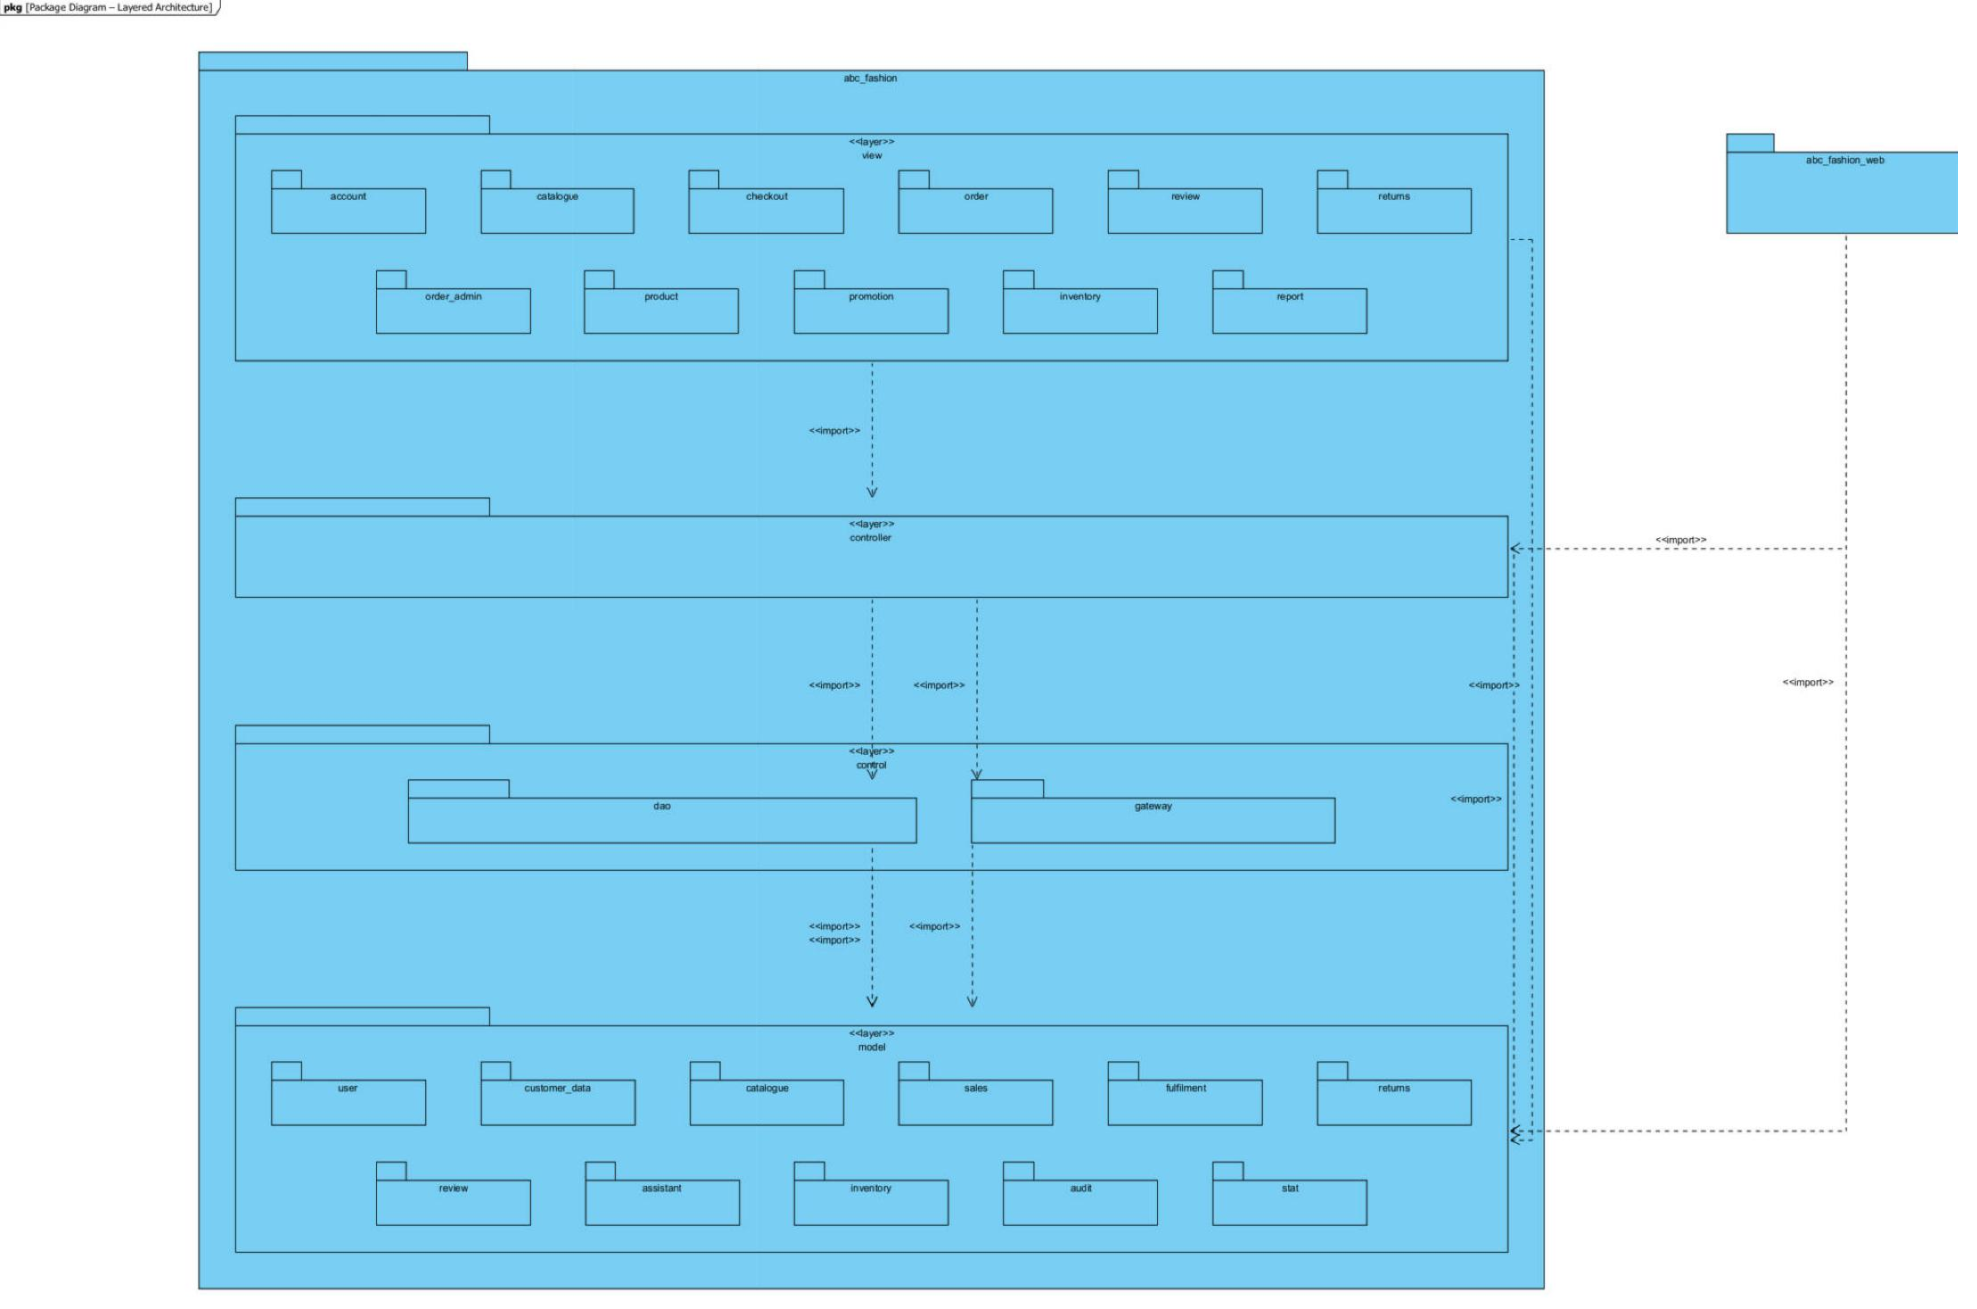
\includegraphics[width=\textwidth,height=0.80\textheight,keepaspectratio]{ly_package.png}
\caption{Package diagram of the MVC architecture --- the layers \texttt{view}, \texttt{controller}, \texttt{control} and \texttt{model} with their sub-packages, the web application \texttt{abc\_fashion\_web} and the \guillemotleft import\guillemotright{} dependencies (Visual Paradigm)}
\label{fig:layers}
\end{figure}

In Figure~\ref{fig:layers} all dependencies point downwards: the view packages and the web application import \texttt{controller} and \texttt{model}; \texttt{controller} imports \texttt{control.dao}, \texttt{control.gateway} and \texttt{model}; \texttt{dao} and \texttt{gateway} import \texttt{model}; the model packages import nothing outside \texttt{model}. The former dependencies from the view packages to \texttt{dao} and \texttt{gateway} were removed.

The layering was chosen for four reasons. First, the SQL is separated from the screens: a change of the database touches only the DAO of the table concerned, and a change of a screen only its \textsf{Frm} class. Second, the business rules and the transactions of a use case are in one controller instead of being spread over the button handlers, so the desktop screens and the web application share them. Third, the external services are reached only through gateways called by controllers, so that a sandbox provider can be replaced by the real one without changing a screen. Fourth, the model layer depends on nothing, so the same entity classes can be used everywhere and tested without a database.

\textbf{Gateway classes.} The design class diagram of Section~\ref{sec:designclass} contains no class for the external systems, although several use cases need them: payment in UC08 and UC31, the carrier in UC28, and the AI functions in UC05 and UC32--UC34. Five gateway classes were therefore added to the package \texttt{control}; they are called only by controllers (Table~\ref{tab:gateways}, Figures~\ref{fig:gateway1} and~\ref{fig:gateway2}).

{\small
\begin{xltabular}{\textwidth}{@{}L{3.1cm} L{5.2cm} Y@{}}
\caption{Gateway classes added to the control layer}\label{tab:gateways}\\
\toprule
\textbf{Gateway} & \textbf{Operations} & \textbf{Used by (controller)} \\ \midrule
\endfirsthead
\toprule
\textbf{Gateway} & \textbf{Operations} & \textbf{Used by (controller)} \\ \midrule
\endhead
\bottomrule
\endlastfoot
\textsf{PaymentGateway} & \texttt{charge(order, method)}, \texttt{refund(payment)}, \texttt{link\_method(customer, type, provider)} & \textsf{CheckoutController}, \textsf{OrderController}, \textsf{OrderAdminController}, \textsf{ReturnController}, \textsf{ProfileController} \\
\textsf{ShippingGateway} & \texttt{create\_shipment(shipment)}, \texttt{get\_tracking(shipment)} & \textsf{OrderController}, \textsf{OrderAdminController}, \textsf{ReturnController}, \textsf{SyncController} \\
\textsf{NotificationGateway} & \texttt{send(notification)} & every controller that calls \texttt{NotificationDAO.add\_notification}, and \textsf{InventoryController} \\
\textsf{SearchEngine} & \texttt{search\_by\_image(image)}, \texttt{search\_by\_voice(audio)}, returning the ids of the matching styles & \textsf{CatalogueController}, \textsf{ProductController}, \textsf{SyncController} \\
\textsf{AssistantEngine} & \texttt{ask(question, style)}, \texttt{summarise\_reviews(style)}, \texttt{moderate(review)} & \textsf{CatalogueController}, \textsf{ReviewController} \\
\end{xltabular}
}

\begin{figure}[H]
\centering
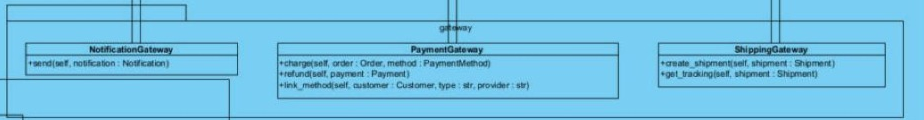
\includegraphics[width=\textwidth]{ly_gateway1.png}
\caption{Gateway classes \textsf{NotificationGateway}, \textsf{PaymentGateway} and \textsf{ShippingGateway} in package \texttt{control.gateway}}
\label{fig:gateway1}
\end{figure}

\begin{figure}[H]
\centering
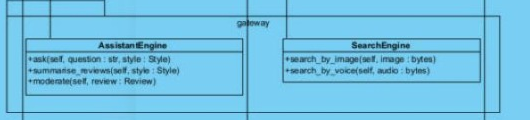
\includegraphics[width=0.62\textwidth]{ly_gateway2.png}
\caption{Gateway classes \textsf{AssistantEngine} and \textsf{SearchEngine}, the entry points to the AI components of Chapter~\ref{ch:ai}}
\label{fig:gateway2}
\end{figure}

\subsection{Packages of the Layers}
\label{subsec:packages}
Inside each layer the classes are grouped in sub-packages (Figure~\ref{fig:layers}). The view layer has one package per functional module, the controller layer one package with the 15 controllers, the package \texttt{control} one sub-package for the DAO classes and one for the gateways, and the model layer the eleven packages of the analysis model (Section~\ref{sec:analysisclass}), each holding the entity classes of a group of tables together with the enumerations they use.


Table~\ref{tab:viewpackages} maps every view package to the use cases it realises and to the controllers its screens call; Table~\ref{tab:modelpackages} lists the model packages.

{\small
\begin{xltabular}{\textwidth}{@{}L{2.0cm} L{4.2cm} L{2.3cm} Y L{1.9cm}@{}}
\caption{View packages, their classes, use cases and the controllers they call}\label{tab:viewpackages}\\
\toprule
\textbf{Package} & \textbf{View classes} & \textbf{Use cases} & \textbf{Controllers called} & \textbf{Gateways (via controller)} \\ \midrule
\endfirsthead
\toprule
\textbf{Package} & \textbf{View classes} & \textbf{Use cases} & \textbf{Controllers called} & \textbf{Gateways (via controller)} \\ \midrule
\endhead
\bottomrule
\endlastfoot
\texttt{account} & LoginFrm, RegisterFrm, CustomerHomeFrm, ProfileFrm, EditAddressFrm, LinkPaymentMethodFrm, AdminHomeFrm, SearchAccountFrm, EditAccountFrm, AuditLogFrm & UC01--UC03, UC20 & AccountAdmin, Auth, Profile & Payment \\
\texttt{catalogue} & BrowseStyleFrm, SearchStyleFrm, StyleDetailFrm, AssistantFrm & UC04--UC06, UC32, UC33 & Cart, Catalogue & Assistant Engine, Search Engine \\
\texttt{checkout} & CartFrm, CheckoutFrm, ConfirmOrderFrm & UC07, UC08, UC25, UC26, UC28--UC31 & Cart, Checkout & Notification, Payment \\
\texttt{order} & OrderListFrm, OrderDetailFrm, TrackShipmentFrm, CancelRequestFrm, ReviewFrm, ReturnRequestFrm & UC09--UC14, UC34 & Order, Return, Review & Assistant Engine, Notification, Payment, Shipping \\
\texttt{order\_admin} & ManagerHomeFrm, SearchOrderFrm, ManageOrderFrm & UC22, UC23 & OrderAdmin & Notification, Payment, Shipping \\
\texttt{product} & ManageStyleFrm, EditStyleFrm, EditVariantFrm & UC21 & Product & Search Engine \\
\texttt{promotion} & MerchandiserHomeFrm, ManagePromotionFrm, EditPromotionFrm, SelectStyleFrm & UC15, UC27 & Promotion & --- \\
\texttt{inventory} & WarehouseHomeFrm, StockLevelFrm, AdjustStockFrm, StockMovementFrm, ManageRestockFrm, EditRestockRequestFrm, SelectVariantFrm, SupplierHomeFrm, ConfirmRestockFrm & UC17 & Inventory & Notification \\
\texttt{returns} & CustomerServiceHomeFrm, SearchReturnRequestFrm, ProcessReturnFrm, InspectReturnFrm & UC18 & Return & Notification, Payment, Shipping \\
\texttt{review} & ManageReviewFrm & UC19 & Review & Assistant Engine \\
\texttt{report} & MarketingHomeFrm, SelectReportFrm, SalesReportFrm, SalesDetailFrm, ReturnReportFrm, ReturnDetailFrm & UC16, UC24 & Report & --- \\
\end{xltabular}
}

{\small
\begin{xltabular}{\textwidth}{@{}L{2.4cm} Y L{5.0cm}@{}}
\caption{Model packages: entity classes and enumerations}\label{tab:modelpackages}\\
\toprule
\textbf{Package} & \textbf{Entity classes} & \textbf{Enumerations} \\ \midrule
\endfirsthead
\toprule
\textbf{Package} & \textbf{Entity classes} & \textbf{Enumerations} \\ \midrule
\endhead
\bottomrule
\endlastfoot
\texttt{user} & User, Customer, StaffMember, Supplier & AccountStatus, StaffRole \\
\texttt{customer\_data} & Address, PaymentMethod, SavedSize, Notification & LinkedMethodType, Channel, NotificationEvent, NotificationStatus \\
\texttt{audit} & AuditLogEntry & AuditAction \\
\texttt{catalogue} & Category, Collection, Style, MaterialComponent, SizeChartEntry, ProductMedia, ProductVariant & FitType, StyleStatus, Season, Measure, MediaType, VariantStatus \\
\texttt{inventory} & StockLocation, StockLevel, StockMovement, RestockRequest, RestockItem & MovementReason, RestockStatus \\
\texttt{sales} & Cart, CartItem, Order, OrderItem, OrderVoucher, Payment, Promotion, PromotionStyle, Voucher & OrderStatus, DeliveryService, DiscountType, PaymentKind, PaymentMethodType, PaymentStatus, PromoType, PromotionStatus \\
\texttt{fulfilment} & Shipment, ShipmentRecord, ShipmentEvent & ShipmentDirection, ShipmentStatus \\
\texttt{returns} & ReturnRequest, ReturnItem, ReturnEvidence & ReturnType, ReturnReason, Resolution, ReturnStatus, InspectionResult \\
\texttt{review} & Review & FitVote, ReviewStatus \\
\texttt{assistant} & AssistantTurn, GroundingEvent & AssistantMode, GroundingCheck \\
\texttt{stat} & StyleStat, ReturnStat (statistic objects, specialisations of Style) & --- \\ \midrule
\textbf{11 packages} & \textbf{41 classes} & \textbf{34 enumerations} \\
\end{xltabular}
}

\subsection{Relations between Layers and Classes}
\label{subsec:layerrelations}
\label{fig:layeredclass}
Figure~\ref{fig:designfull} in Section~\ref{sec:designclass} is the complete class diagram with the classes placed in their layer packages: from top to bottom the view layer, the controller layer, the package \texttt{control} with the gateways and the DAO classes, and the model layer; Figures~\ref{fig:design1}--\ref{fig:design7} show each band at a readable size. All connectors are drawn orthogonally, and every relationship crosses the layer boundaries only from top to bottom. Table~\ref{tab:layerrelations} counts the relationships of the model by kind and by the layers they connect.

{\small
\begin{xltabular}{\textwidth}{@{}L{3.3cm} L{3.6cm} r Y@{}}
\caption{Relationships between the layers and inside them}\label{tab:layerrelations}\\
\toprule
\textbf{Kind} & \textbf{From $\rightarrow$ to} & \textbf{Number} & \textbf{Meaning and example} \\ \midrule
\endfirsthead
\toprule
\textbf{Kind} & \textbf{From $\rightarrow$ to} & \textbf{Number} & \textbf{Meaning and example} \\ \midrule
\endhead
\bottomrule
\endlastfoot
Association & view $\rightarrow$ view & 63 & Navigation: a screen opens the next one (\textsf{LoginFrm} opens the home screen of every role; \textsf{CartFrm} $\rightarrow$ \textsf{CheckoutFrm} $\rightarrow$ \textsf{ConfirmOrderFrm}) \\
Association & view $\rightarrow$ controller & 46 & A screen sends the user's request to its controller (\textsf{CheckoutFrm} $\rightarrow$ \textsf{CheckoutController}) \\
Association & controller $\rightarrow$ control.dao & 82 & A controller reads and writes tables (\textsf{CheckoutController} $\rightarrow$ \textsf{OrderDAO}) \\
Association & controller $\rightarrow$ control.gateway & 20 & A controller calls an external service (\textsf{CheckoutController} $\rightarrow$ \textsf{PaymentGateway}) \\
Association & control.dao $\rightarrow$ model & 33 & A DAO reads and writes the rows of its entity (\textsf{OrderDAO} $\rightarrow$ \textsf{Order}) \\
Generalisation & control.dao $\rightarrow$ control.dao & 33 & Every DAO inherits the base class \textsf{DAO}, which owns the database connection \\
Composition & model $\rightarrow$ model & 16 & Parts that cannot exist without their whole (\textsf{OrderItem} in \textsf{Order}) \\
Aggregation / association & model $\rightarrow$ model & 34 & References between entities through a foreign key (\textsf{Order} -- \textsf{Customer}) \\
Generalisation & model $\rightarrow$ model & 8 & \textsf{User} $\leftarrow$ \textsf{Customer}, \textsf{StaffMember}, \textsf{Supplier}; \textsf{ProductVariant} $\leftarrow$ \textsf{CartItem} $\leftarrow$ \textsf{OrderItem} $\leftarrow$ \textsf{ReturnItem}; \textsf{Style} $\leftarrow$ \textsf{StyleStat}, \textsf{ReturnStat} \\
Usage \guillemotleft use\guillemotright & model $\rightarrow$ model & 39 & An entity uses an enumeration as the type of an attribute (\textsf{Order} $\rightarrow$ \textsf{OrderStatus}) \\
Dependency \guillemotleft import\guillemotright & package $\rightarrow$ package & --- & The package dependencies of Figure~\ref{fig:layers} \\
\end{xltabular}
}

The relationships obey three rules. (1) Calls go only downwards: a view knows the views it opens and its controller; a controller knows the DAO and gateway classes it uses; a DAO knows only its entity; an entity knows neither views, controllers nor DAOs. There is no relationship from a view to a DAO, a gateway or an entity class: a screen keeps the entities in typed attributes and receives them as parameters, which the package dependency \texttt{view} $\rightarrow$ \texttt{model} expresses. (2) Only the DAO classes touch the database, through the connection of the base class \textsf{DAO}, and only the gateway classes touch the external systems; both are used only by controllers. (3) Objects move between the layers as entity objects: \textsf{CheckoutController} returns an \textsf{Order} to \textsf{CheckoutFrm}, which passes it to \textsf{ConfirmOrderFrm}, so no layer needs to know how another layer stores or shows the data. Section~\ref{subsec:verification} checks these rules automatically on the code.

\subsection{Use-Case Views of the Layers}
\label{subsec:slices}
A diagram with all 182 classes is too large to read at once. The layers are therefore also shown in five \emph{use-case views} (Figures~\ref{fig:slicecheckout}--\ref{fig:slicebackoffice}). Each view is a class diagram of the same model that contains only the classes of one group of use cases, arranged in the four bands view -- controller -- control -- model, with all their attributes, operations and relationships. The classes of each band are placed in one or two rows, chosen for every view so that the figure fills a landscape page as fully as possible, and all connectors are drawn with right angles.

\subsubsection*{L1 --- Place Order (UC07, UC08, UC25, UC26, UC29, UC31)}
\label{subsec:slicecheckout}
Figure~\ref{fig:slicecheckout} contains 3 view classes, the controllers \textsf{CartController} and \textsf{CheckoutController}, 9 DAO classes with the base class \textsf{DAO}, 2 gateways and 13 entity classes. \textsf{CartFrm} shows the cart with \texttt{CartController.get\_cart()}, changes quantities with \texttt{update\_quantity()} and \texttt{remove\_item()}, and before \texttt{on\_checkout()} opens \textsf{CheckoutFrm} it calls \texttt{check\_availability()}, which asks \texttt{StockLevelDAO} (UC29). \textsf{CheckoutFrm} calls \texttt{CheckoutController.start\_checkout()}, which builds the draft order with the automatic promotion prices (\textsf{PromotionDAO}); \texttt{on\_apply\_voucher()} calls \texttt{apply\_voucher()}, which reads the code with \texttt{VoucherDAO.get\_voucher\_by\_code()} (UC26), and \texttt{on\_place\_order()} calls \texttt{place\_order()}. The controller checks the address and the payment method and calls \texttt{OrderDAO.add\_order()}, which in one database transaction inserts the \textsf{Order} with its \textsf{OrderItem} and \textsf{OrderVoucher} rows and reserves the stock with \texttt{SELECT \ldots{} FOR UPDATE}, so that two customers can never buy the last unit at the same time (UC29, NFR10); if any step fails the transaction is rolled back (NFR07). Only after the commit does the controller call \texttt{PaymentGateway.charge()} (UC31), record the result with \texttt{PaymentDAO.add\_payment()} and confirm the order with \texttt{NotificationDAO} and \texttt{NotificationGateway}. \textsf{ConfirmOrderFrm} reads the order again with \texttt{get\_order()}; if the payment failed, \texttt{on\_retry\_payment()} calls \texttt{retry\_payment()}.

\begin{landscape}
\begin{figure}[p]
\centering
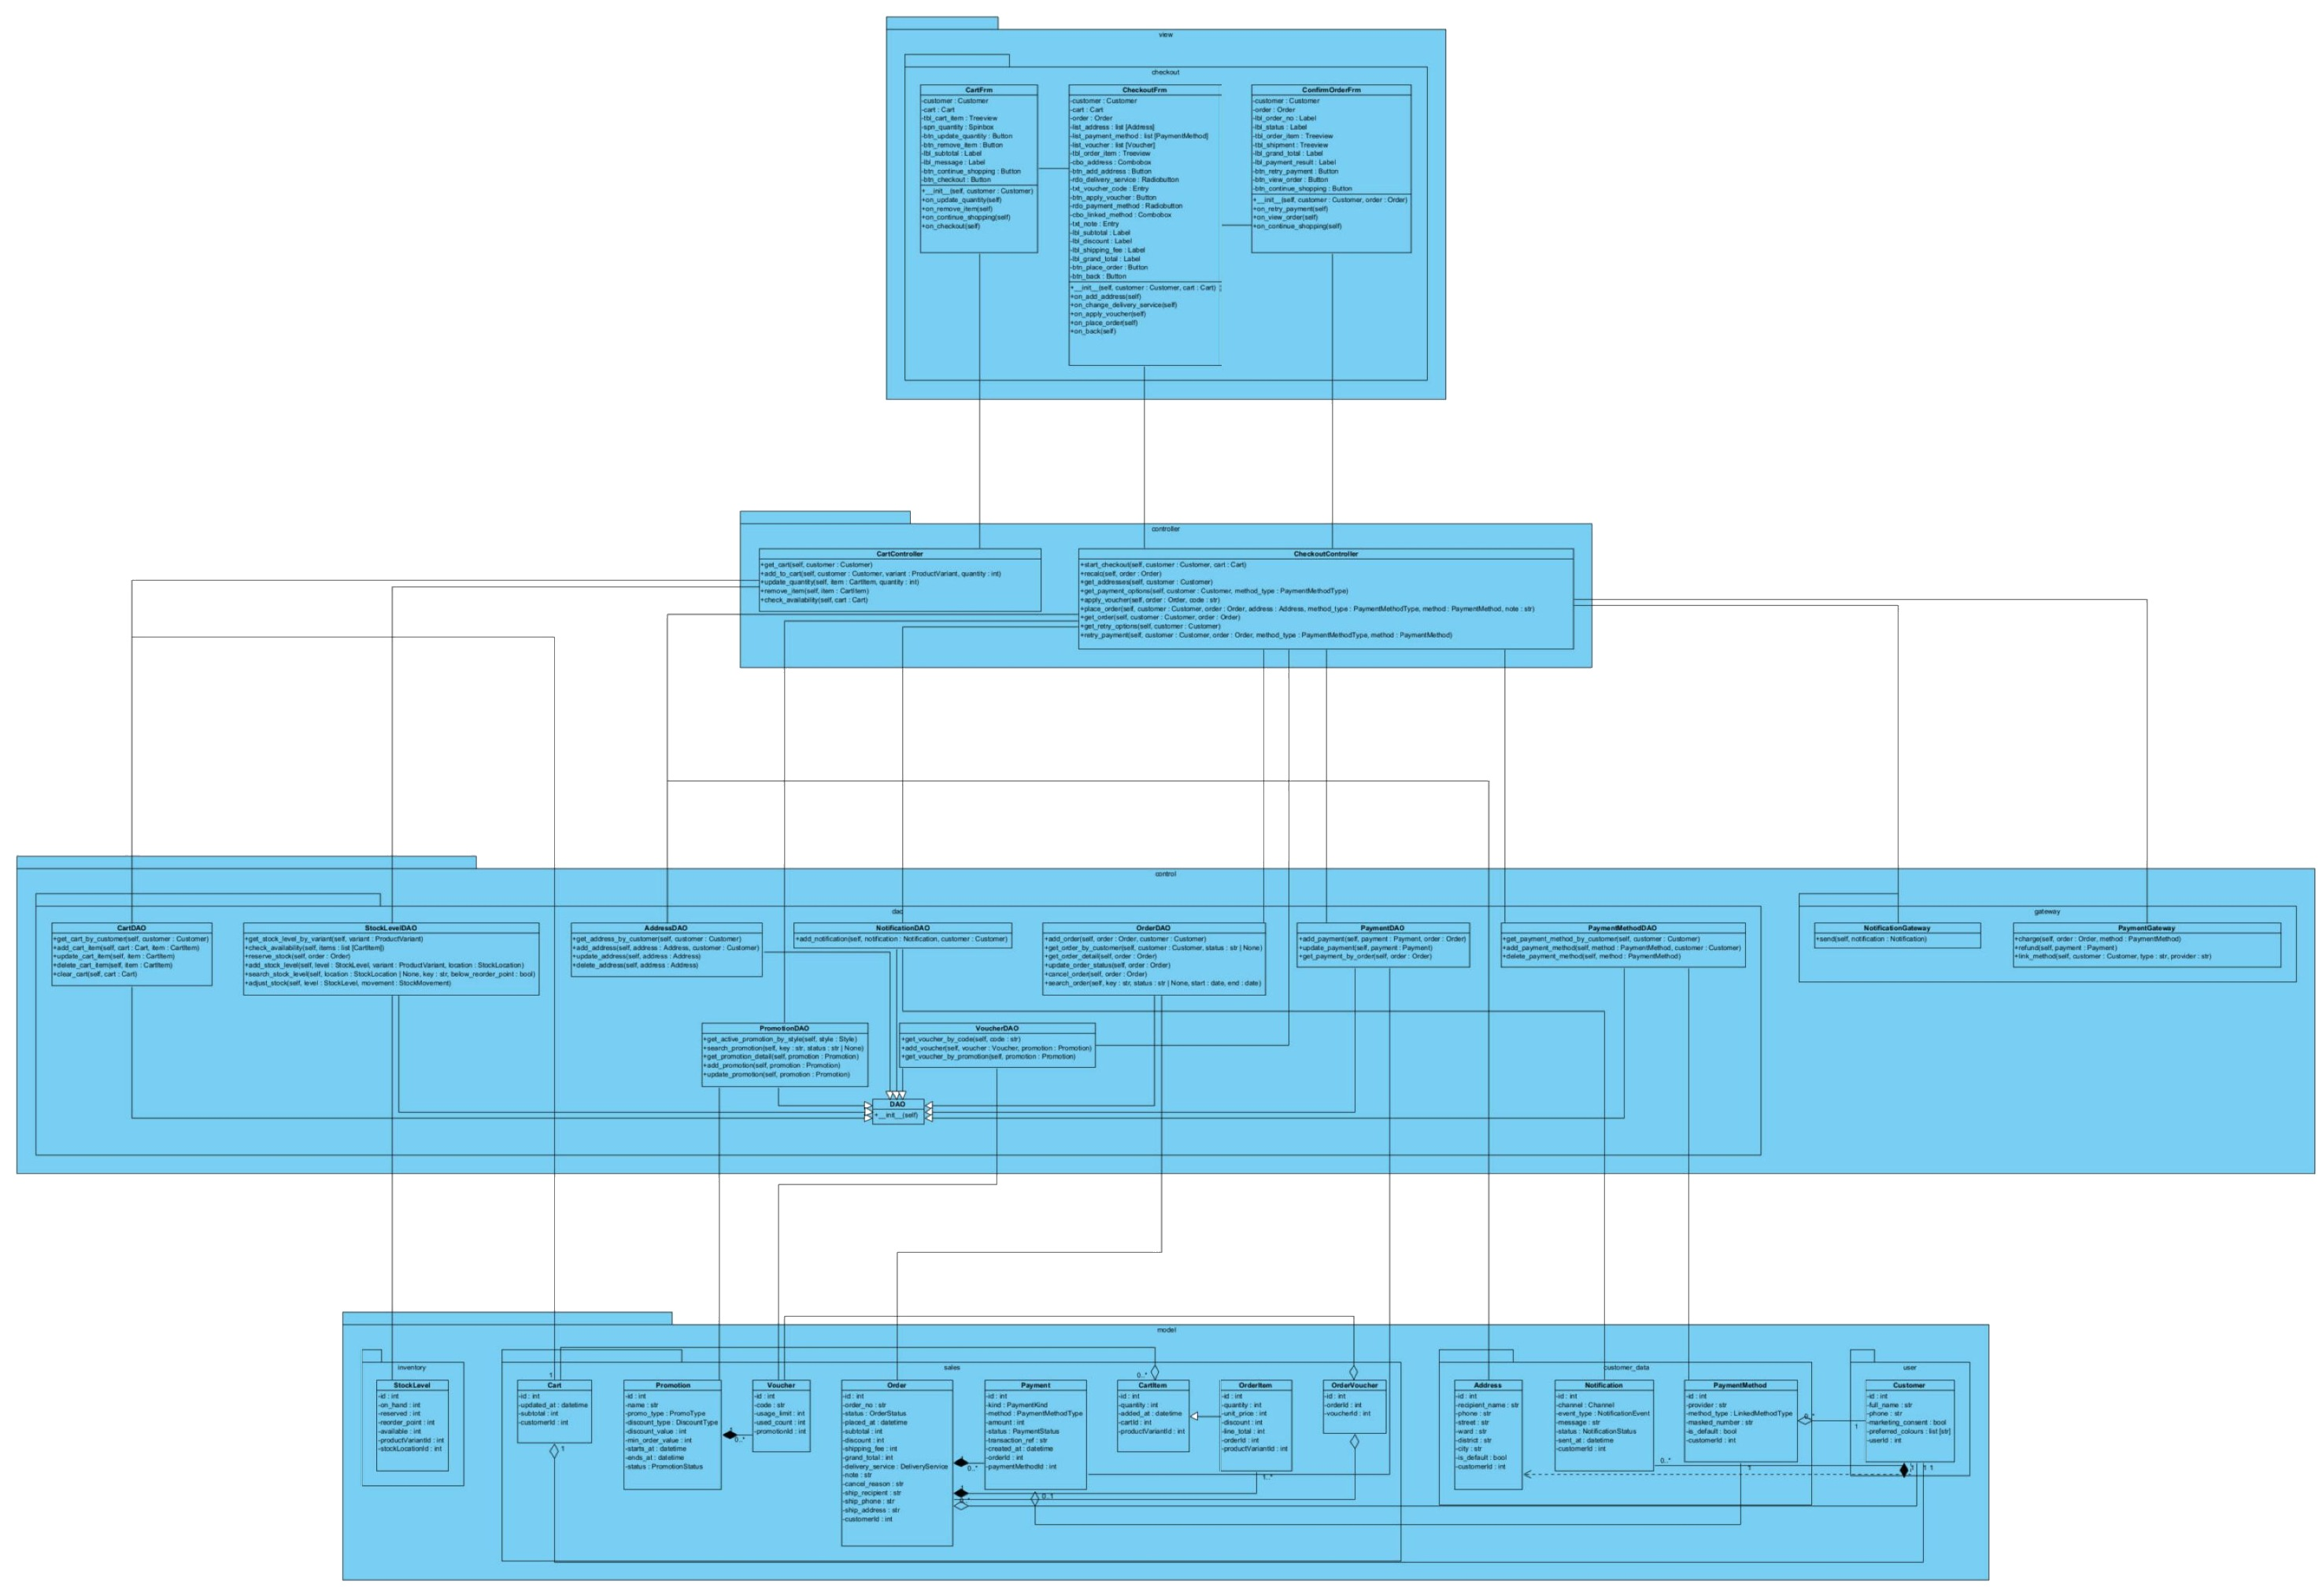
\includegraphics[width=\linewidth,height=0.92\textheight,keepaspectratio]{ly_l1_place_order.jpg}
\caption{Layered view L1 --- place order: \textsf{CartFrm}, \textsf{CheckoutFrm}, \textsf{ConfirmOrderFrm} with their controllers, DAO classes, gateways and entities}
\label{fig:slicecheckout}
\end{figure}
\end{landscape}

\subsubsection*{L2 --- Request and Process Return / Exchange (UC14, UC18)}
Figure~\ref{fig:slicereturns} contains 6 view classes, the controllers \textsf{OrderController} and \textsf{ReturnController}, 8 DAO classes, 3 gateways and 14 entity classes. The customer starts from \textsf{OrderDetailFrm}, which reads the order with \texttt{OrderController.get\_order\_detail()}; \texttt{on\_return()} opens \textsf{ReturnRequestFrm}, where the items, the reason, the replacement variant of an exchange (\texttt{ReturnController.get\_replacement\_options()}) and the photos (\textsf{ReturnEvidence}) are entered; \texttt{on\_submit()} calls \texttt{submit\_return\_request()}, which stores the request with \texttt{ReturnRequestDAO.add\_return\_request()}. Customer-service staff find it in \textsf{SearchReturnRequestFrm} and decide in \textsf{ProcessReturnFrm}: \texttt{authorise()} and \texttt{reject()} update the request; \texttt{create\_pickup()} creates the return parcel with \texttt{ShipmentDAO} and \texttt{ShippingGateway}; \texttt{refund()} calls \texttt{PaymentGateway.refund()} and records the refund with \texttt{PaymentDAO}; \texttt{ship\_replacement()} sends the new size or colour and takes it out of stock with \texttt{StockLevelDAO}. Warehouse staff record the inspection in \textsf{InspectReturnFrm} (\texttt{save\_inspection()}, \texttt{finish\_inspection()}); a passed item goes back into stock with \texttt{StockLevelDAO.adjust\_stock()}, which writes a \textsf{StockMovement} with reason \emph{return} in the same transaction. Each decision is announced to the customer through \textsf{NotificationDAO} and \textsf{NotificationGateway}.

\begin{landscape}
\begin{figure}[p]
\centering
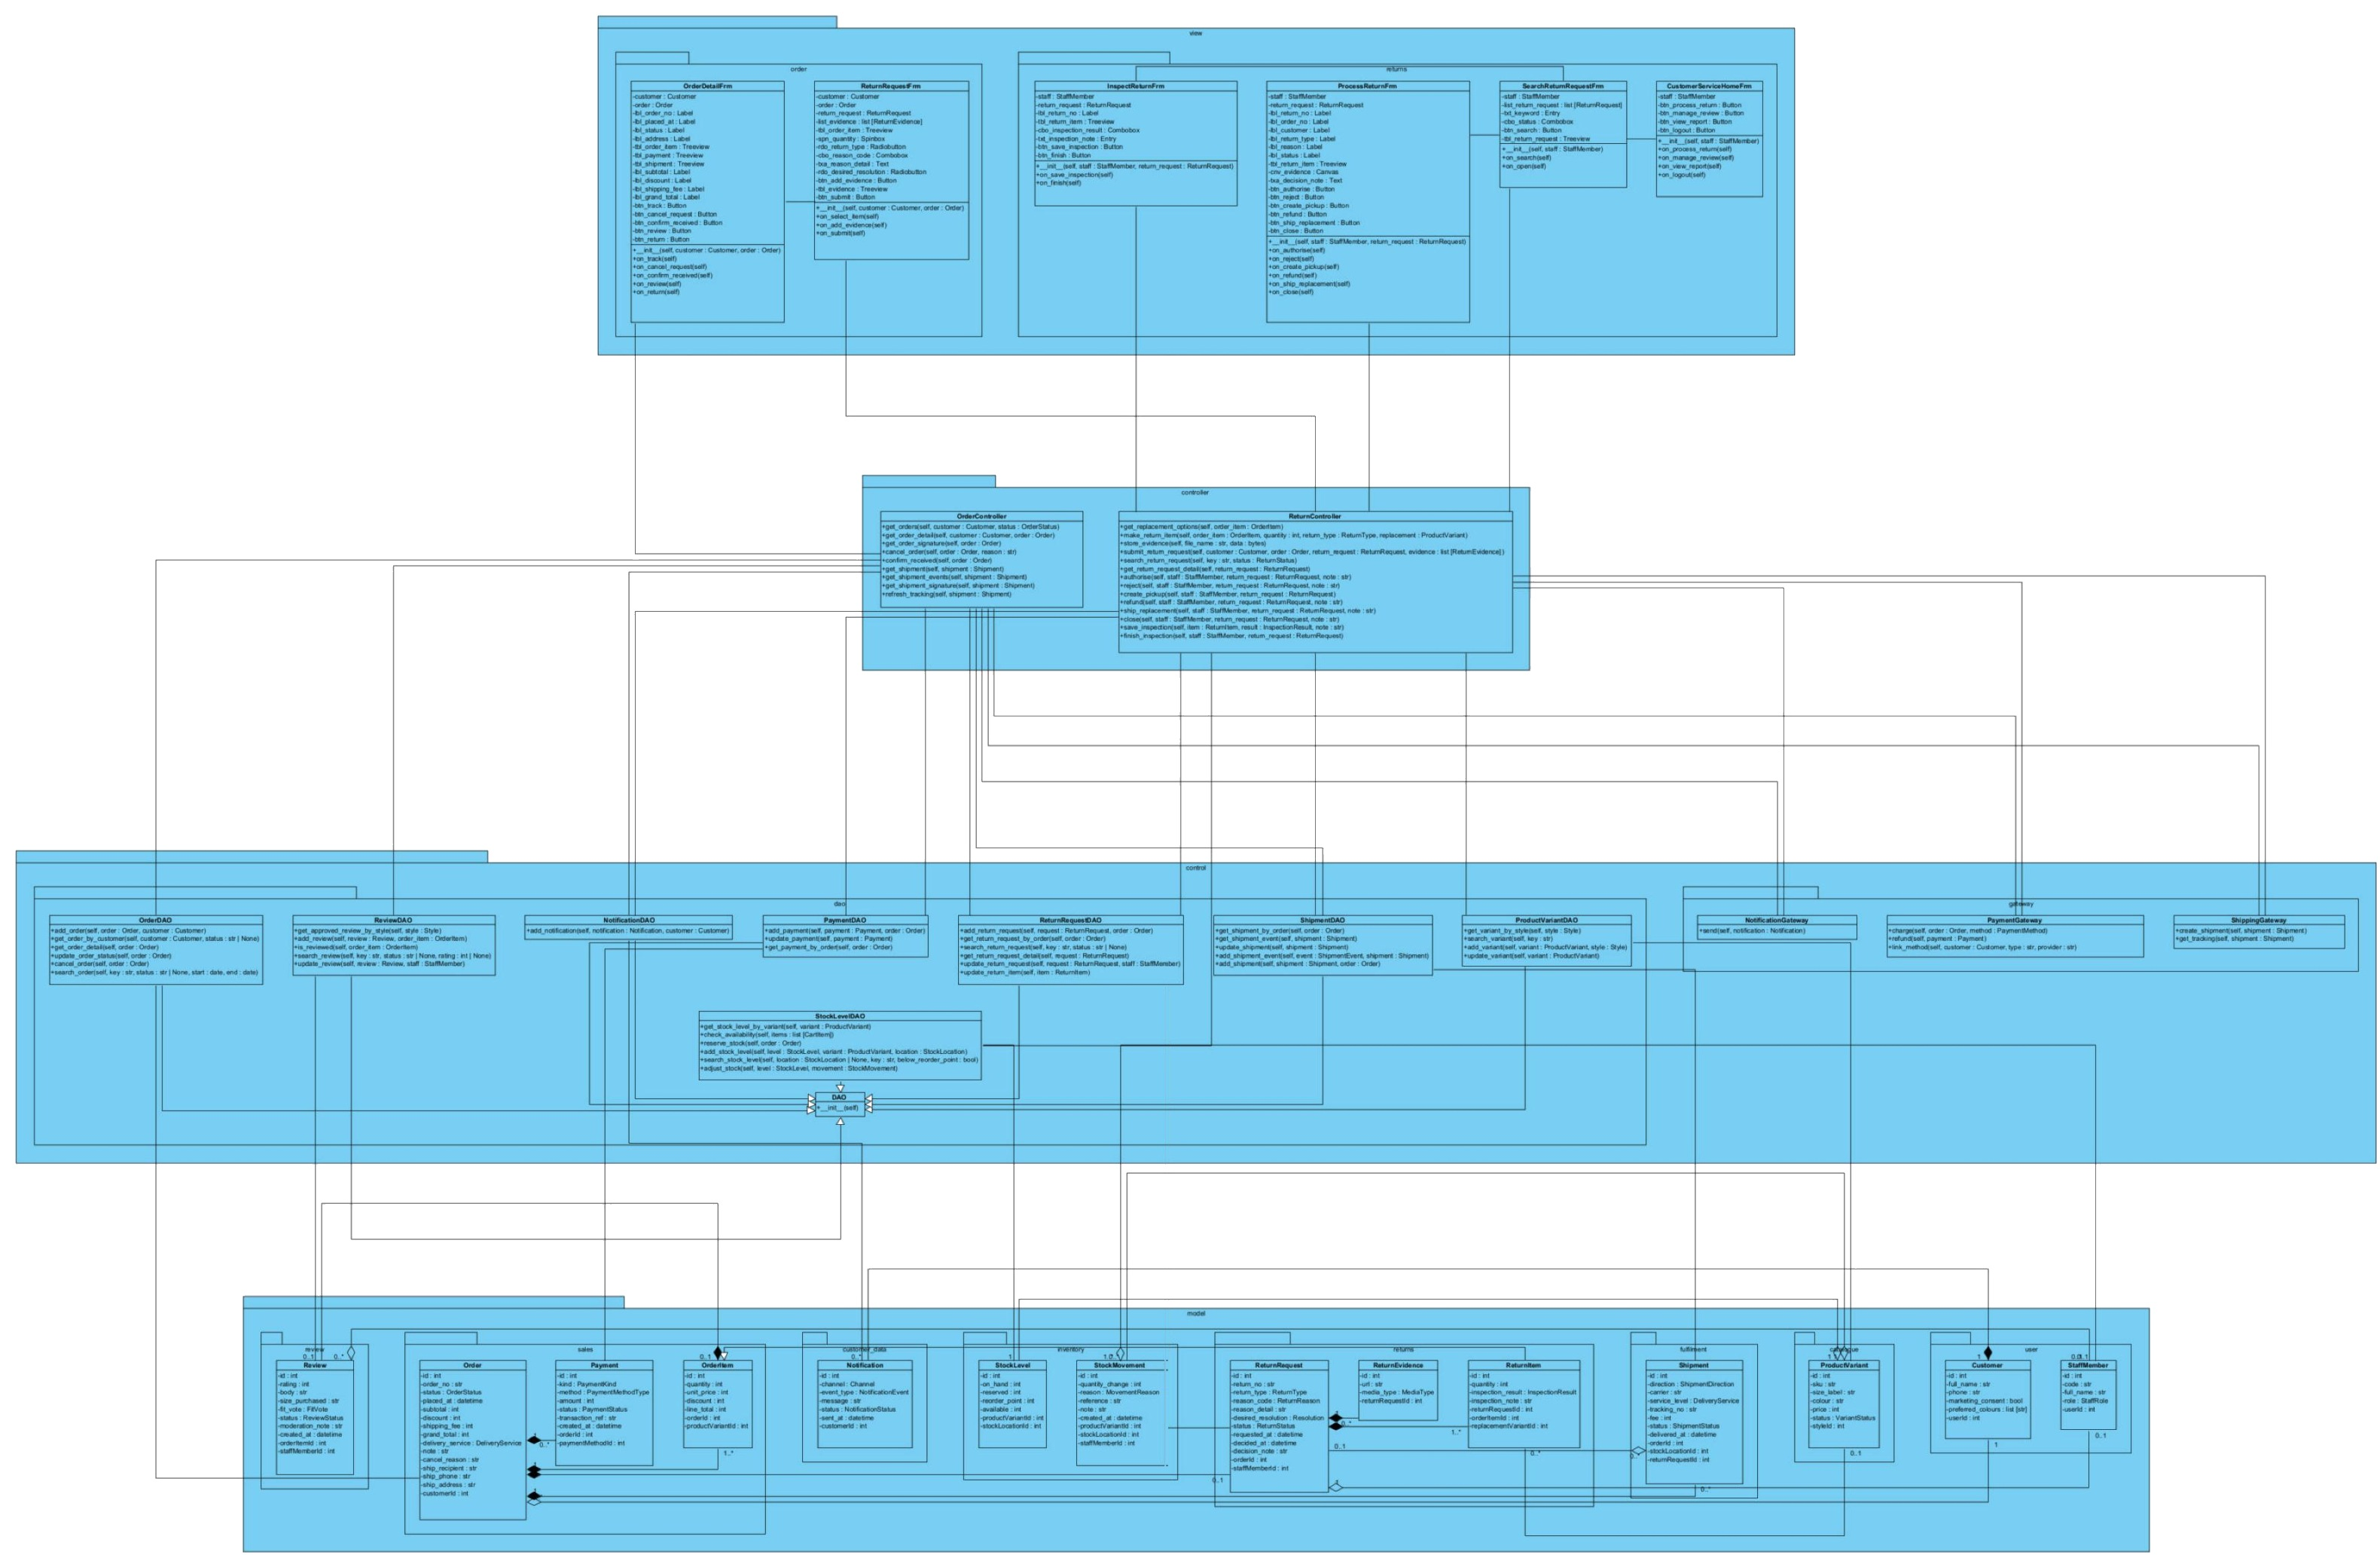
\includegraphics[width=\linewidth,height=0.92\textheight,keepaspectratio]{ly_l2_returns.jpg}
\caption{Layered view L2 --- return and exchange: customer request, processing by customer service and inspection in the warehouse}
\label{fig:slicereturns}
\end{figure}
\end{landscape}

\subsubsection*{L3 --- Catalogue and AI Assistant (UC04--UC06, UC32, UC33)}
Figure~\ref{fig:slicesearch} connects the AI components of Chapter~\ref{ch:ai} with the catalogue through \textsf{CatalogueController} and \textsf{CartController}. \textsf{BrowseStyleFrm} shows the category tree (\texttt{get\_categories()}) and filters styles with \texttt{browse\_style()}, which calls \texttt{StyleDAO.get\_style\_by\_category()}. \textsf{SearchStyleFrm} searches by keyword with \texttt{search\_style()}; for a photo or a spoken query the controller calls \texttt{SearchEngine.search\_by\_image()} or \texttt{search\_by\_voice()}, which return the ids of the matching styles, and reads these styles with \texttt{StyleDAO.search\_style\_by\_ids()}. \textsf{StyleDetailFrm} assembles the product page from \texttt{get\_style\_detail()} (style, variants, media, material, size chart), \texttt{get\_stock\_level()}, \texttt{get\_final\_price()} with the active promotion and \texttt{summarise\_reviews()}, which passes the approved reviews to \texttt{AssistantEngine.summarise\_reviews()} (UC33); \texttt{on\_add\_to\_cart()} calls \texttt{CartController.add\_to\_cart()}. \textsf{AssistantFrm} sends the question to \texttt{ask\_assistant()}, which gives \texttt{AssistantEngine.ask()} the real data of the style, and logs the answer with \texttt{save\_assistant\_turn()} and \texttt{AssistantTurnDAO}; the checks applied to the answer are stored as \textsf{GroundingEvent} rows (UC32).

\begin{landscape}
\begin{figure}[p]
\centering
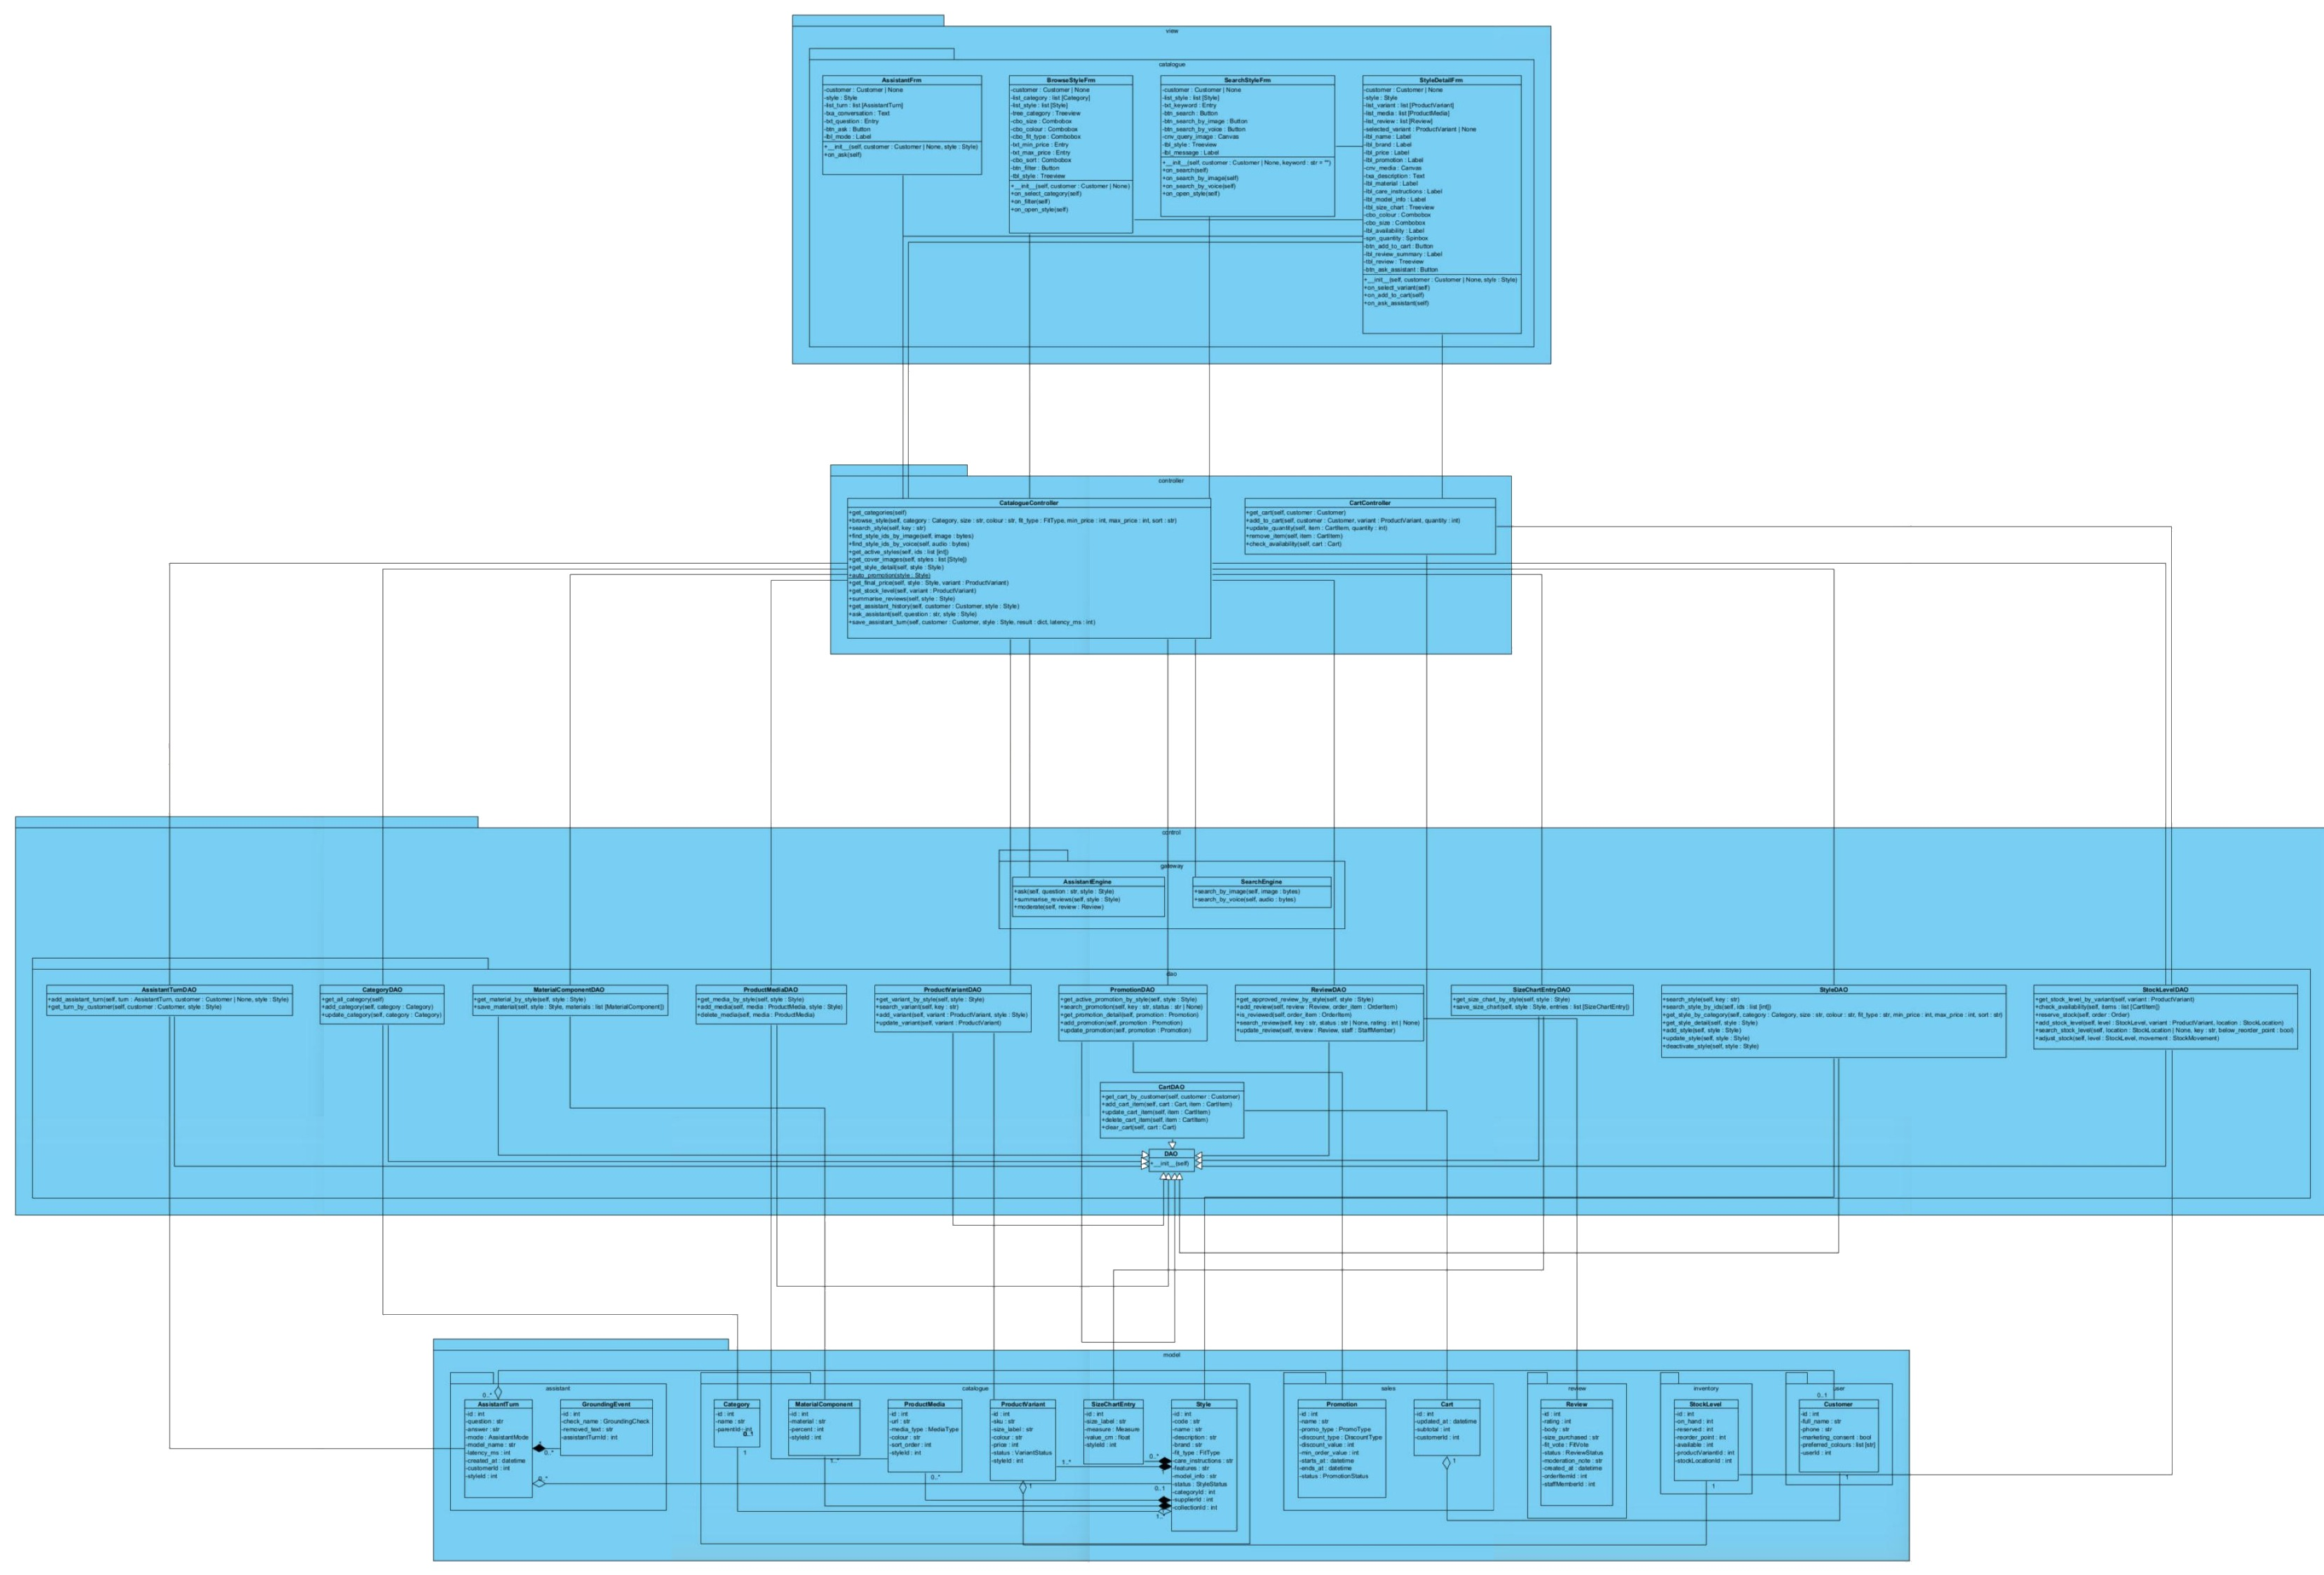
\includegraphics[width=\linewidth,height=0.92\textheight,keepaspectratio]{ly_l3_catalogue_assistant.jpg}
\caption{Layered view L3 --- catalogue, search and AI assistant: views, controllers, DAO classes, the gateways \textsf{SearchEngine} and \textsf{AssistantEngine}, and entities}
\label{fig:slicesearch}
\end{figure}
\end{landscape}

\subsubsection*{L4 --- Inventory and Restocking (UC17)}
Figure~\ref{fig:sliceinventory} contains the nine screens of package \texttt{view.inventory}, all served by \textsf{InventoryController}. \textsf{StockLevelFrm} lists the stock per warehouse with \texttt{search\_stock\_level()} and \texttt{get\_stock\_locations()}, optionally only the rows below the reorder point. \textsf{AdjustStockFrm} calls \texttt{adjust\_stock()} with a mandatory reference and reason; the controller changes the \textsf{StockLevel}, writes the \textsf{StockMovement} in one transaction (NFR11) and records an \textsf{AuditLogEntry}. \textsf{StockMovementFrm} shows the movements of a variant (\texttt{get\_movements()}). \textsf{ManageRestockFrm} and \textsf{EditRestockRequestFrm} create and send restock requests (\texttt{search\_restock\_request()}, \texttt{save\_restock\_request()}, with \texttt{get\_suppliers()} and the variants chosen in \textsf{SelectVariantFrm}); sending a request e-mails the supplier through \textsf{NotificationGateway}. The supplier answers in \textsf{SupplierHomeFrm} and \textsf{ConfirmRestockFrm} (\texttt{confirm\_restock()}, \texttt{refuse\_restock()}). When the goods arrive, \texttt{receive\_restock()} increases the stock and writes one \emph{restock} movement per item.

\begin{landscape}
\begin{figure}[p]
\centering
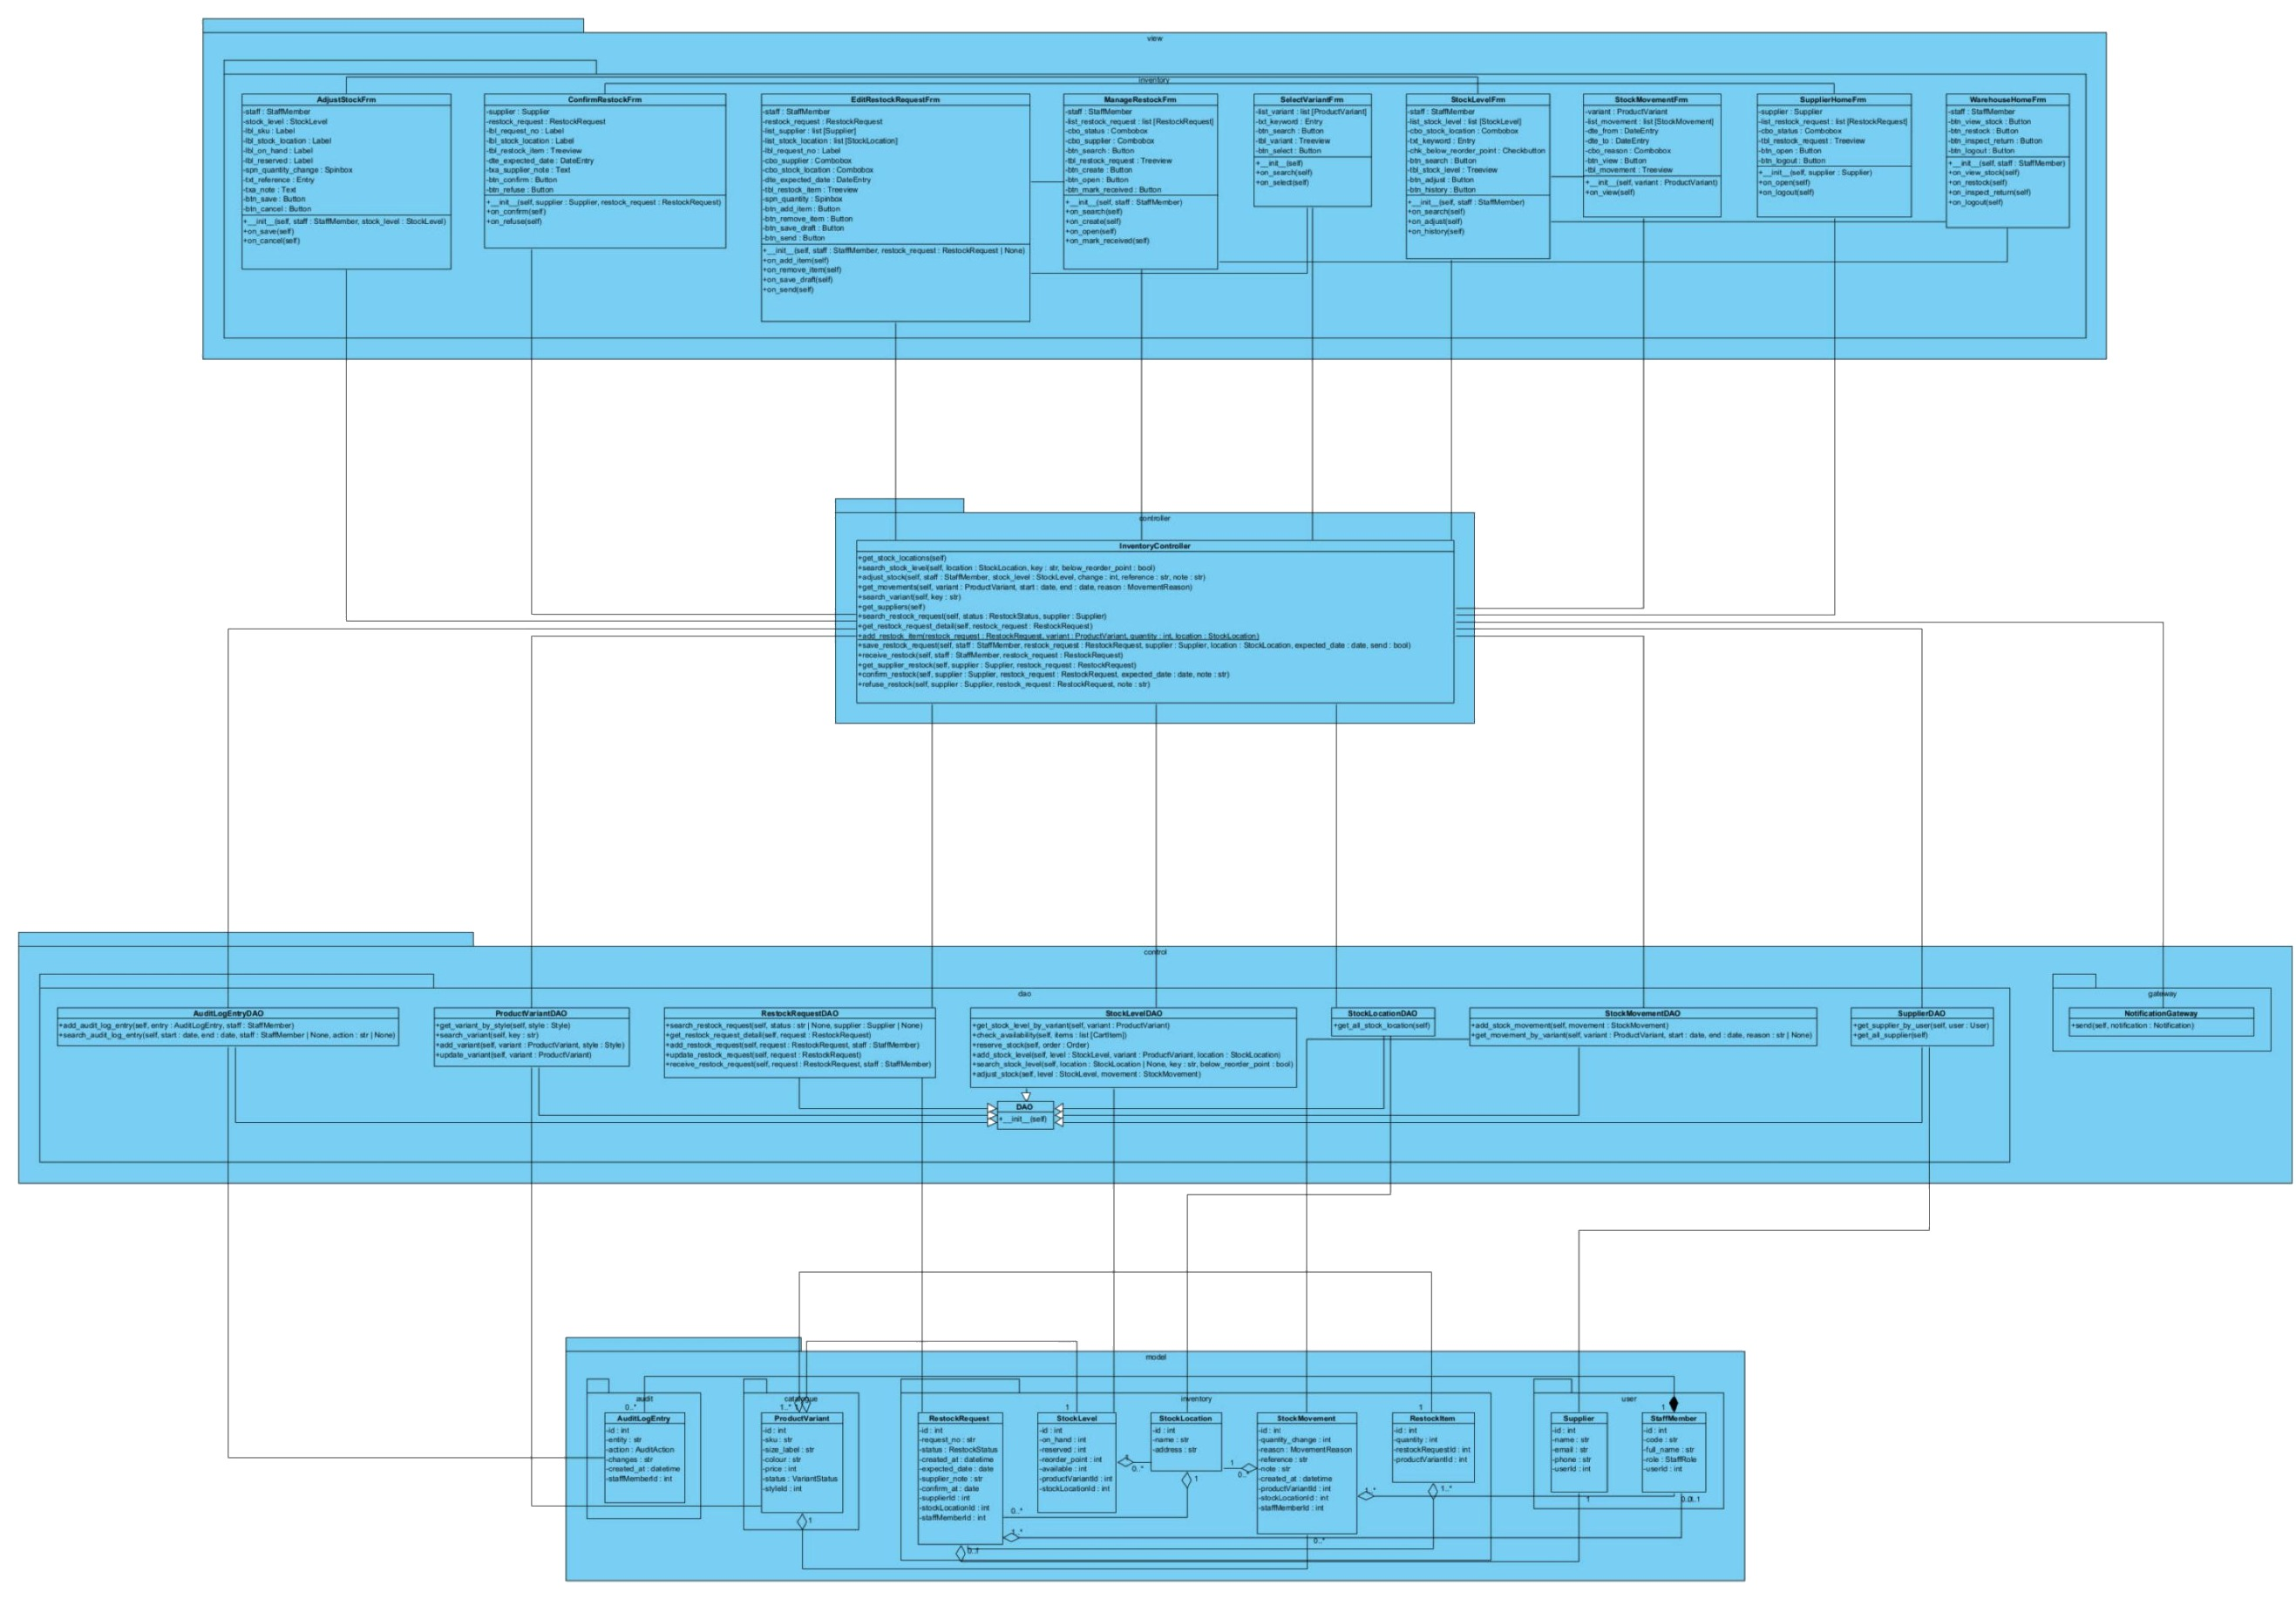
\includegraphics[width=\linewidth,height=0.92\textheight,keepaspectratio]{ly_l4_inventory.jpg}
\caption{Layered view L4 --- inventory and restocking: warehouse and supplier screens, \textsf{InventoryController}, inventory DAO classes and entities}
\label{fig:sliceinventory}
\end{figure}
\end{landscape}

\subsubsection*{L5 --- Back-Office: Accounts, Products, Promotions and Reports (UC15, UC16, UC20, UC21, UC24, UC27)}
Figure~\ref{fig:slicebackoffice} is the largest view, with 17 screens and four controllers. The administrator manages the accounts in \textsf{SearchAccountFrm} and \textsf{EditAccountFrm} through \textsf{AccountAdminController} (\texttt{search\_user()}, \texttt{suspend\_account()}, \texttt{activate\_account()}, \texttt{reset\_password()}, \texttt{change\_role()}), each change being written to the audit log, which \textsf{AuditLogFrm} reads with \texttt{search\_audit\_log()}. \textsf{ManageStyleFrm}, \textsf{EditStyleFrm} and \textsf{EditVariantFrm} maintain a style with its variants, media, material composition and size chart through \textsf{ProductController} (\texttt{save\_style()}, \texttt{upload\_media()}, \texttt{save\_variant()}), which uses the seven catalogue DAO classes, creates the stock row of a new variant (\texttt{StockLevelDAO.add\_stock\_level()}) and updates the search index of \textsf{SearchEngine}. The merchandiser defines promotions and vouchers in \textsf{ManagePromotionFrm} and \textsf{EditPromotionFrm} through \textsf{PromotionController} and chooses the styles in \textsf{SelectStyleFrm}. The marketing staff open the reports through \textsf{ReportController}: \texttt{get\_sales\_report()} returns \textsf{StyleStat} objects from \texttt{StyleStatDAO} for \textsf{SalesReportFrm}, \texttt{get\_return\_report()} returns \textsf{ReturnStat} objects from \texttt{ReturnStatDAO} for \textsf{ReturnReportFrm}, and the detail screens list the order items and return items (Figure~\ref{fig:statclasses}).

\begin{landscape}
\begin{figure}[p]
\centering
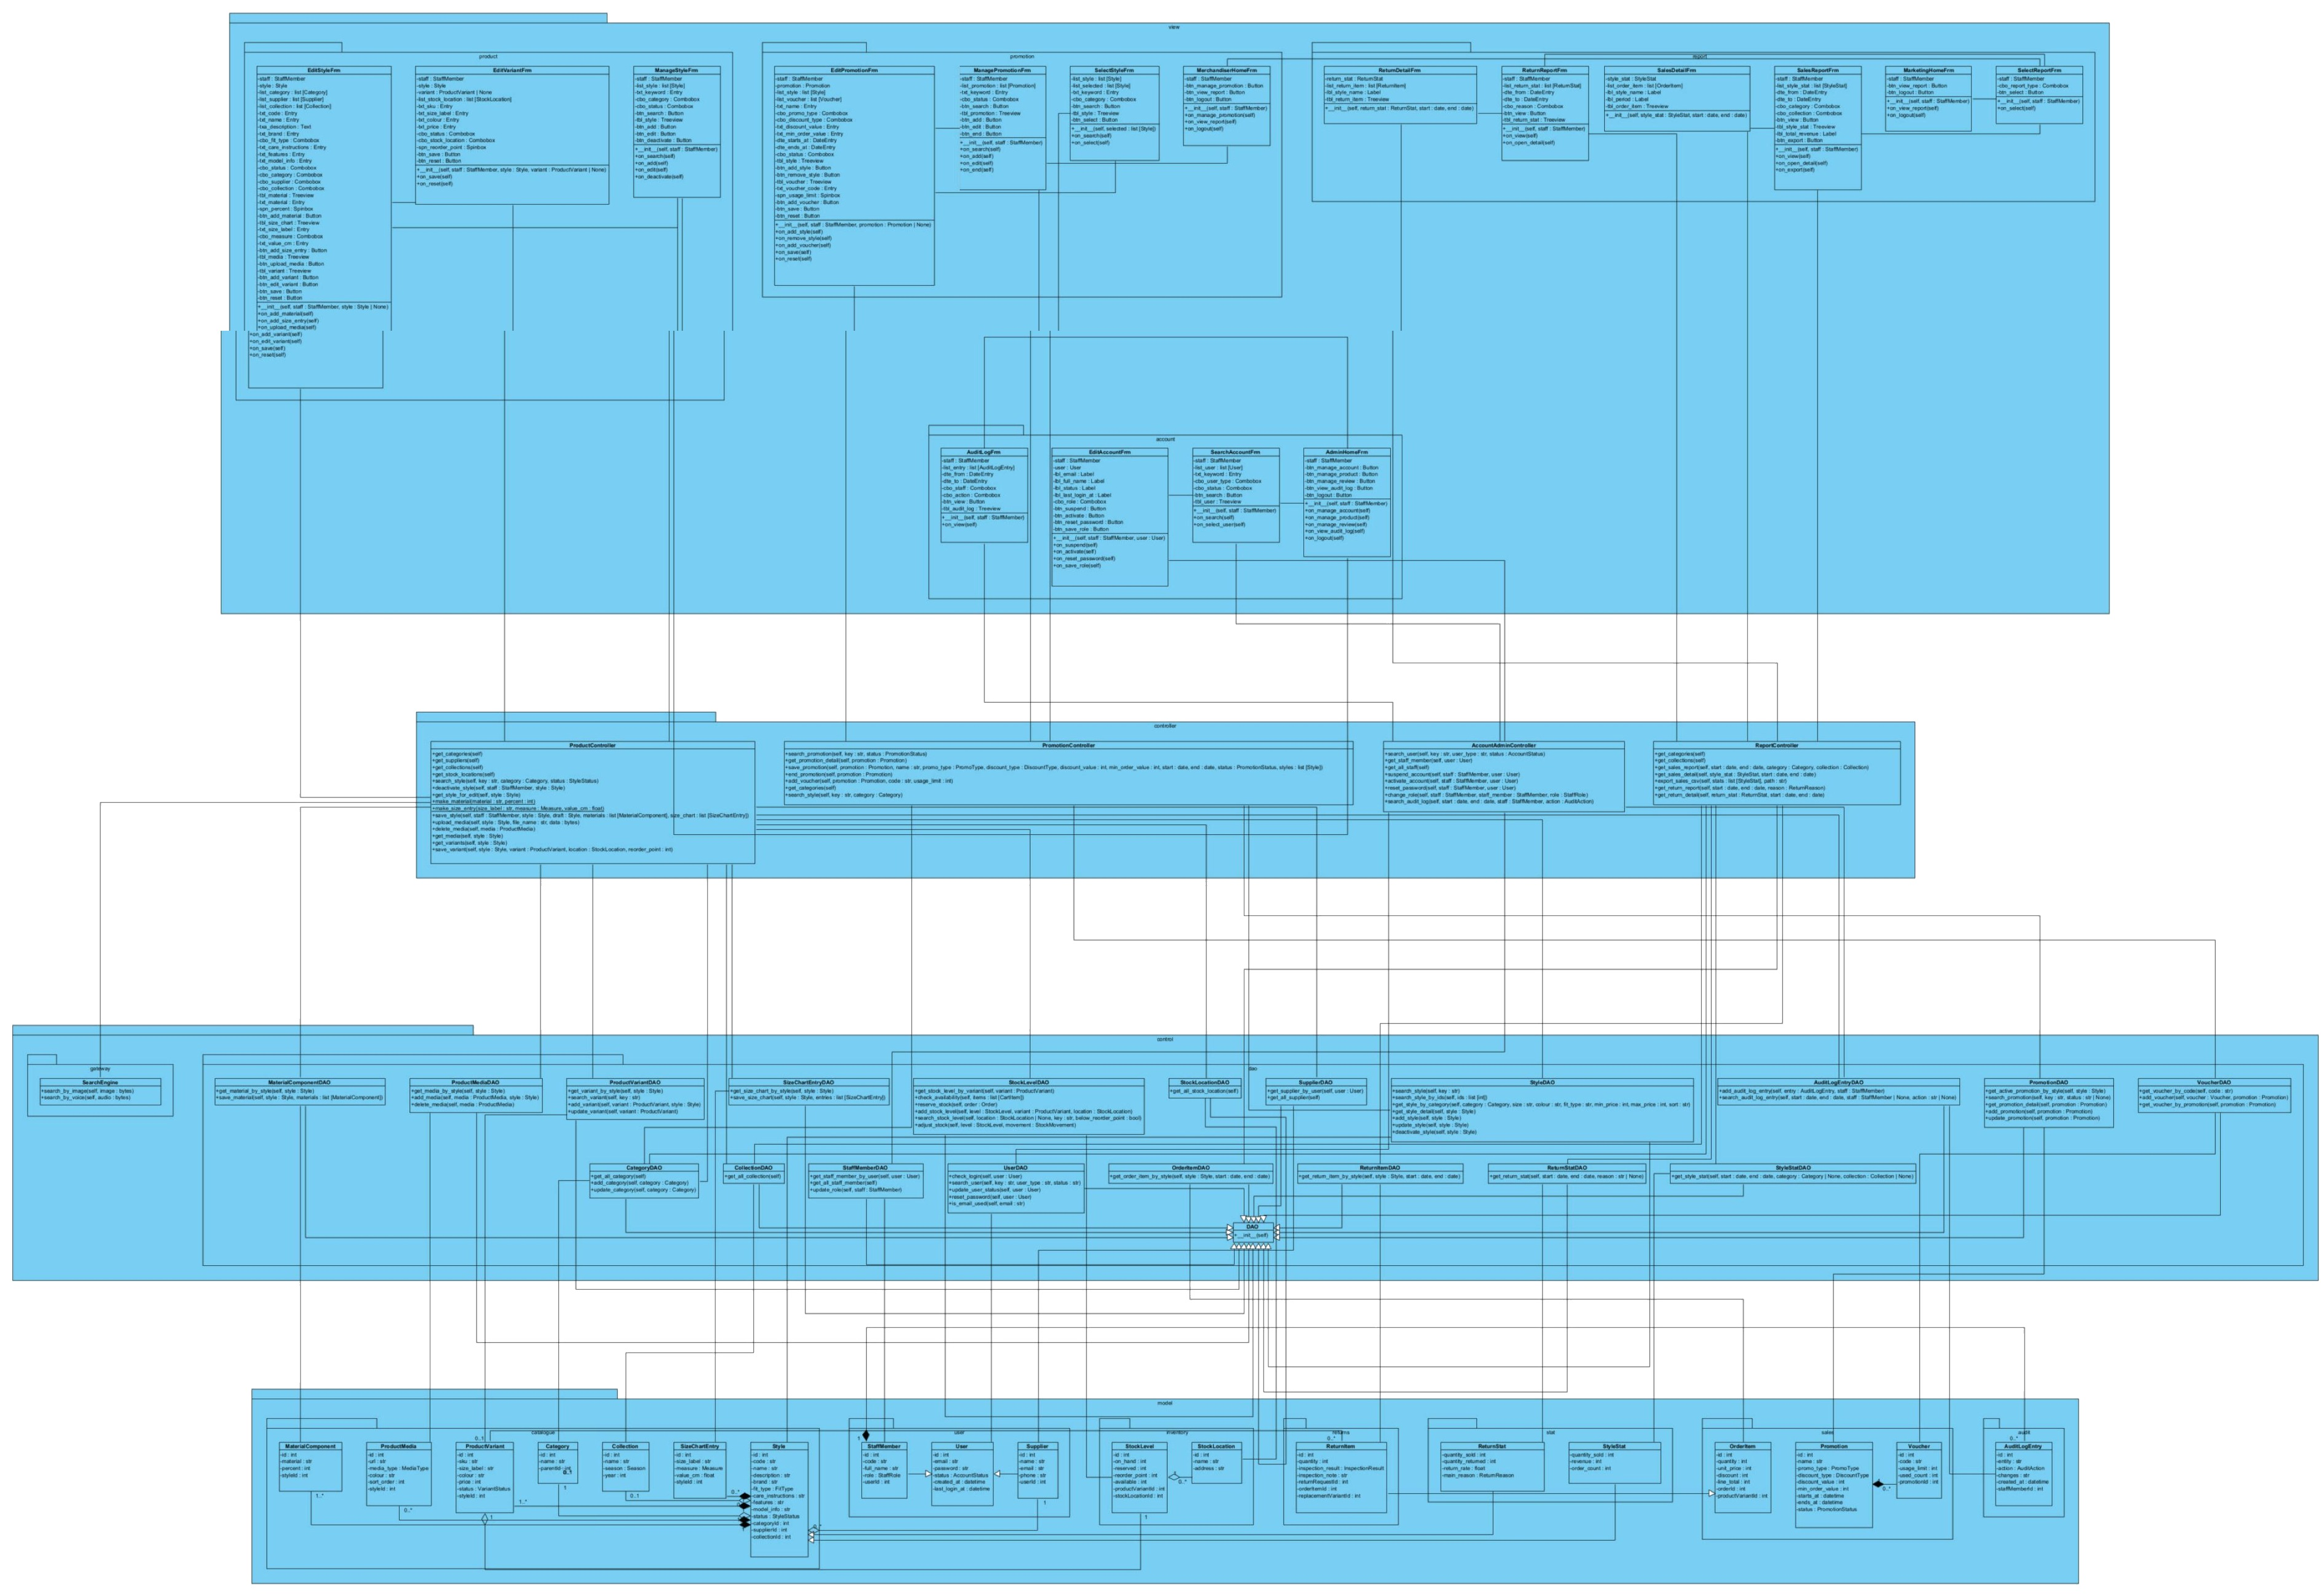
\includegraphics[width=\linewidth,height=0.92\textheight,keepaspectratio]{ly_l5_backoffice.jpg}
\caption{Layered view L5 --- back-office: accounts, products, promotions and reports}
\label{fig:slicebackoffice}
\end{figure}
\end{landscape}

\begin{figure}[H]
\centering
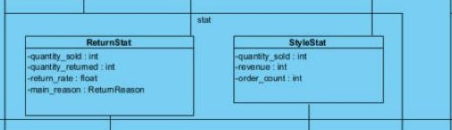
\includegraphics[width=0.55\textwidth]{ly_stat.png}
\caption{Statistic classes \textsf{ReturnStat} and \textsf{StyleStat} in package \texttt{model.stat}}
\label{fig:statclasses}
\end{figure}

\subsection{Component Diagram}
\label{subsec:component}
The component diagram (Figure~\ref{fig:component}) shows the system one level above the classes: the deployable parts, the interfaces between them and the external systems. The whole Python application is the subsystem \textsf{ABC Fashion Application}. Inside it, seven UI components group the view packages and \textsf{ABC Fashion Web} is the customer web application; six controller components group the 15 controllers and provide one \emph{service} interface each; six data-access components group the DAO classes and provide the data interfaces; \textsf{Integration Gateways} provides the interfaces to the external systems. The UI components require only service interfaces, so the diagram shows the same rule as the class diagram: a screen never reaches the data or the external services directly. Table~\ref{tab:components} lists the components and Table~\ref{tab:interfaces} the interfaces.

\begin{landscape}
\begin{figure}[p]
\centering
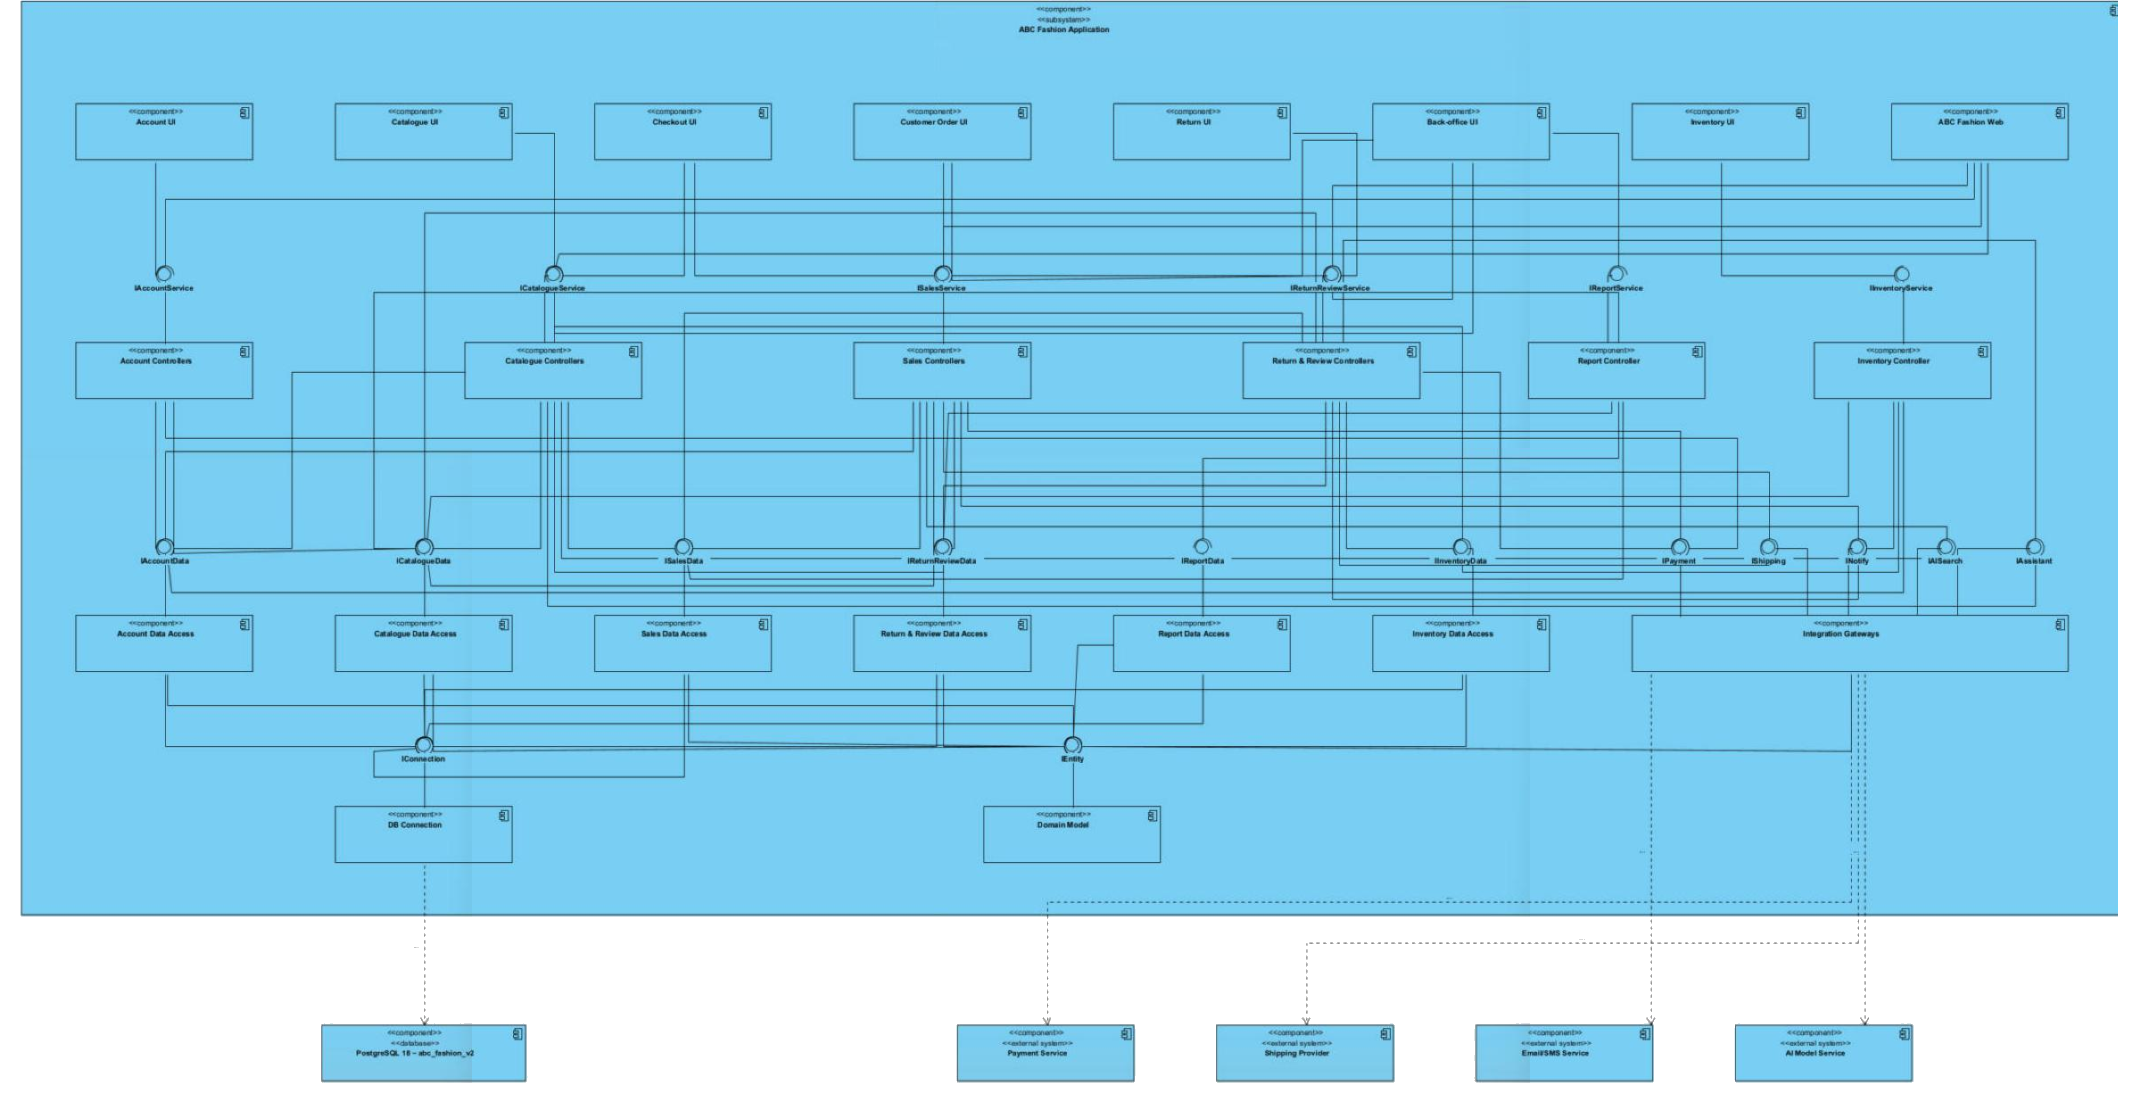
\includegraphics[width=\linewidth,height=0.90\textheight,keepaspectratio]{ly_component.png}
\caption{Component diagram of ABC Fashion IS --- UI, controller, data-access and gateway components with their provided and required interfaces, the database and the external systems (Visual Paradigm)}
\label{fig:component}
\end{figure}
\end{landscape}

{\small
\begin{xltabular}{\textwidth}{@{}r L{4.2cm} L{2.4cm} Y@{}}
\caption{Components of ABC Fashion IS}\label{tab:components}\\
\toprule
\textbf{\#} & \textbf{Component} & \textbf{Stereotype} & \textbf{Contains} \\ \midrule
\endfirsthead
\toprule
\textbf{\#} & \textbf{Component} & \textbf{Stereotype} & \textbf{Contains} \\ \midrule
\endhead
\bottomrule
\endlastfoot
1 & ABC Fashion Application & subsystem & components 2--24 \\
2--8 & Account UI, Catalogue UI, Checkout UI, Customer Order UI, Back-office UI, Inventory UI, Return UI & component & the view packages: \texttt{account}; \texttt{catalogue}; \texttt{checkout}; \texttt{order}; \texttt{order\_admin}, \texttt{product}, \texttt{promotion}, \texttt{review}, \texttt{report}; \texttt{inventory}; \texttt{returns} \\
9 & ABC Fashion Web & component & the customer web application \texttt{abc\_fashion\_web} (routes and HTML templates) \\
10 & Account Controllers & component & \textsf{AuthController}, \textsf{ProfileController}, \textsf{AccountAdminController} \\
11 & Catalogue Controllers & component & \textsf{CatalogueController}, \textsf{CartController}, \textsf{ProductController} \\
12 & Sales Controllers & component & \textsf{CheckoutController}, \textsf{OrderController}, \textsf{OrderAdminController}, \textsf{PromotionController}, \textsf{SyncController} \\
13 & Inventory Controller & component & \textsf{InventoryController} \\
14 & Return \& Review Controllers & component & \textsf{ReturnController}, \textsf{ReviewController} \\
15 & Report Controller & component & \textsf{ReportController} \\
16 & Account Data Access & component & User, Customer, StaffMember, Supplier, Address, PaymentMethod, SavedSize, AuditLogEntry DAO \\
17 & Catalogue Data Access & component & Category, Collection, Style, ProductVariant, ProductMedia, MaterialComponent, SizeChartEntry DAO \\
18 & Inventory Data Access & component & StockLocation, StockLevel, StockMovement, RestockRequest DAO \\
19 & Sales Data Access & component & Cart, Promotion, Voucher, Order, OrderItem, Payment, Shipment, Notification DAO \\
20 & Return \& Review Data Access & component & ReturnRequest, ReturnItem, Review, AssistantTurn DAO \\
21 & Report Data Access & component & StyleStat, ReturnStat DAO \\
22 & DB Connection & component & the base class \textsf{DAO} \\
23 & Domain Model & component & the whole \texttt{model} layer (41 entity classes, 34 enumerations) \\
24 & Integration Gateways & component & the five gateway classes \\
25 & PostgreSQL 18 -- abc\_fashion\_v2 & database & the 39 tables \\
26--29 & Payment Service, Shipping Provider, Email/SMS Service, AI Model Service & external system & sandbox payment provider, carrier, message service, models of Chapter~\ref{ch:ai} \\
\end{xltabular}
}

{\small
\begin{xltabular}{\textwidth}{@{}L{2.9cm} L{2.8cm} L{3.2cm} Y@{}}
\caption{Interfaces of the component diagram}\label{tab:interfaces}\\
\toprule
\textbf{Interface} & \textbf{Provided by} & \textbf{Required by} & \textbf{Operations} \\ \midrule
\endfirsthead
\toprule
\textbf{Interface} & \textbf{Provided by} & \textbf{Required by} & \textbf{Operations} \\ \midrule
\endhead
\bottomrule
\endlastfoot
\textsf{IAccountService} & Account Controllers & Account UI, ABC Fashion Web & login, register, update\_profile, save\_address, link\_payment\_method, search\_user, reset\_password, search\_audit\_log \\
\textsf{ICatalogueService} & Catalogue Controllers & Catalogue, Checkout, Back-office UI, ABC Fashion Web & browse\_style, search\_style, find\_style\_ids\_by\_image, get\_style\_detail, ask\_assistant, add\_to\_cart, check\_availability, save\_style, save\_variant \\
\textsf{ISalesService} & Sales Controllers & Checkout, Customer Order, Back-office UI, ABC Fashion Web & start\_checkout, apply\_voucher, place\_order, retry\_payment, get\_orders, cancel\_order, update\_status, save\_promotion, release\_expired\_orders \\
\textsf{IInventoryService} & Inventory Controller & Inventory UI & search\_stock\_level, adjust\_stock, save\_restock\_request, receive\_restock, confirm\_restock \\
\textsf{IReturnReviewService} & Return \& Review Controllers & Customer Order, Return, Back-office UI, ABC Fashion Web & submit\_return\_request, authorise, create\_pickup, refund, finish\_inspection, submit\_review, moderate\_review \\
\textsf{IReportService} & Report Controller & Back-office UI & get\_sales\_report, get\_sales\_detail, export\_sales\_csv, get\_return\_report, get\_return\_detail \\
\textsf{IAccountData}, \textsf{ICatalogueData}, \textsf{IInventoryData}, \textsf{ISalesData}, \textsf{IReturnReviewData}, \textsf{IReportData} & the six data-access components & the controller components that use their DAO classes & the operations of the DAO classes of Table~\ref{tab:operations} \\
\textsf{IConnection} & DB Connection & all data-access components & \_\_init\_\_ (open the connection), transaction, commit, rollback \\
\textsf{IEntity} & Domain Model & data-access components & the entity classes \\
\textsf{IPayment}, \textsf{IShipping}, \textsf{INotify}, \textsf{IAISearch}, \textsf{IAssistant} & Integration Gateways & the controller components of Table~\ref{tab:gateways} & charge, refund, link\_method; create\_shipment, get\_tracking; send; search\_by\_image, search\_by\_voice; ask, summarise\_reviews, moderate \\
SQL / TCP 5432 & PostgreSQL 18 & DB Connection & --- \\
REST API & the four external systems & Integration Gateways & --- \\
\end{xltabular}
}

The operations of every service interface are operations of the controllers inside the component, and those of every data interface are operations of its DAO classes, so the component diagram is consistent with the class diagram. A provided interface is drawn as a ball attached to its component by a realisation, a required interface as a socket attached by a usage dependency.

\textbf{One use case through the components.} Placing an order (L1) crosses the components as follows: Checkout UI requires \textsf{ISalesService}; Sales Controllers require \textsf{ISalesData} to store the order, \textsf{ICatalogueData} for the promotion prices, \textsf{IPayment} to charge the customer and \textsf{INotify} to confirm the order; Sales Data Access requires \textsf{IConnection}, through which DB Connection reaches PostgreSQL over SQL/TCP port 5432, and Integration Gateways call the Payment Service and the Email/SMS Service over their REST APIs. All components exchange \textsf{Cart}, \textsf{Order} and \textsf{Payment} objects of the Domain Model.

\subsection{How the Design Meets the Non-Functional Requirements}
\label{subsec:nfrdesign}
{\small
\begin{xltabular}{\textwidth}{@{}L{2.4cm} Y@{}}
\caption{Design decisions for the non-functional requirements}\label{tab:nfrdesign}\\
\toprule
\textbf{Requirement} & \textbf{Design decision} \\ \midrule
\endfirsthead
\toprule
\textbf{Requirement} & \textbf{Design decision} \\ \midrule
\endhead
\bottomrule
\endlastfoot
NFR01, NFR02 & Each screen reads its data with one controller call that uses a small, fixed number of DAO operations; indexes on the foreign keys used by browsing and order look-up \\
NFR03 & \textsf{AuthController.login()} identifies the user once and \textsf{LoginFrm} passes the \textsf{Customer} or \textsf{StaffMember} object to the screens it opens; every controller operation of a customer receives this object, filters by it and refuses another customer's order (\texttt{OrderController.get\_order\_detail(customer, order)}) \\
NFR04 & Card data go only to the Payment Service through \textsf{PaymentGateway}; the database stores the provider's token and the masked number (\textsf{PaymentMethod}) \\
NFR07 & Operations that change several tables (\texttt{add\_order}, \texttt{adjust\_stock}, \texttt{receive\_restock}) run in one transaction of the shared connection of class \textsf{DAO}, opened by the DAO or by the controller: commit at the end, rollback on any error; external services are called only after the commit \\
NFR09 & Layers with downward dependencies only: a change of a table touches its entity class and its DAO; a change of a business rule touches one controller; a new carrier or payment provider is a change of one gateway class \\
NFR10 & \texttt{StockLevelDAO.reserve\_stock()} locks the stock rows (\texttt{SELECT \ldots{} FOR UPDATE}); the table refuses \texttt{reserved > on\_hand} \\
NFR11 & Every stock change goes through \textsf{StockLevelDAO} and writes a \textsf{StockMovement} in the same transaction \\
NFR12 & The cart is stored in the database (\textsf{Cart}, \textsf{CartItem}), not on the client \\
NFR13--NFR16 & AI functions only behind \textsf{SearchEngine} and \textsf{AssistantEngine}; \texttt{moderate()} before a review or a question is stored or sent to a model; each answer and its checks are logged (\textsf{AssistantTurn}, \textsf{GroundingEvent}) \\
\end{xltabular}
}

% =====================================================================
\section{Implementation of the Layered Design}
\label{sec:code}

\subsection{From the Model to the Code}
\label{subsec:forward}
The system was programmed in Python on the basis of the Visual Paradigm model of Section~\ref{sec:layers}; the complete source code is kept in the repository \url{https://github.com/DongDucNguyen/PTTKHTTT} (folder \texttt{code}). The model and the code are kept consistent in four steps:
\begin{enumerate}
  \item \textbf{Design model.} The Visual Paradigm project contains the layers \texttt{view}, \texttt{controller}, \texttt{control} and \texttt{model} with 29 packages (including \texttt{abc\_fashion}), 182 classes with typed attributes and 459 operations, and all relationships of Table~\ref{tab:layerrelations}. It is exported with \emph{Project $\rightarrow$ Export $\rightarrow$ XML} into one file (\texttt{project.xml}).
  \item \textbf{Skeleton.} The script \texttt{vp2py.py} reads this XML file and writes one Python module per class of the view, controller and control layers and one module per package of the model layer, following the rules of Table~\ref{tab:codemapping}: names, types, parameters, generalisations and associations are copied from the model.
  \item \textbf{Implementation.} The bodies of the operations were then programmed by hand: SQL in the DAO classes, the use-case logic in the controllers, the calls of the external APIs in the gateways and the widgets in the view classes. Helper modules whose names start with an underscore (for example \texttt{controller/\_flows.py}, \texttt{controller/\_errors.py} with the class \textsf{BusinessError}) are implementation details and are not drawn in the model.
  \item \textbf{Verification.} \texttt{vp2py.py --check} compares the exported model with the programmed code, and \texttt{check\_gen.py} imports every module and applies the layer rules of Table~\ref{tab:layers} to the import statements (Section~\ref{subsec:verification}). A change of the design is therefore made first in Visual Paradigm and then checked against the code.
\end{enumerate}

{\small
\begin{xltabular}{\textwidth}{@{}L{4.0cm} Y@{}}
\caption{Rules for mapping the UML model to Python code}\label{tab:codemapping}\\
\toprule
\textbf{UML element} & \textbf{Python code} \\ \midrule
\endfirsthead
\toprule
\textbf{UML element} & \textbf{Python code} \\ \midrule
\endhead
\bottomrule
\endlastfoot
Package (layer, sub-package) & Python package: a directory with \texttt{\_\_init\_\_.py} (\texttt{abc\_fashion/view/checkout/}) \\
View class \textsf{XxxFrm} & Module \texttt{xxx\_frm.py} with \texttt{class XxxFrm(tk.Toplevel)}: every screen is a window of \texttt{tkinter} \\
Controller, DAO and gateway class & One module per class (\texttt{checkout\_controller.py}, \texttt{order\_dao.py}, \texttt{payment\_gateway.py}) \\
Entity class, enumeration & One module per model package; entity $\rightarrow$ \texttt{@dataclass(kw\_only=True)} with the analysis name of the class (\texttt{class Order}), enumeration $\rightarrow$ \texttt{Enum} whose values are the lower-case literals stored in the database \\
Attribute \texttt{-name : Type} & Typed attribute \texttt{name: Type}; type modifiers give \texttt{list[Address]} and \texttt{X | None} \\
Operation & Method with the designed parameters and types; class-scope operations become \texttt{@staticmethod} \\
Generalisation & Inheritance: \texttt{class OrderDAO(DAO)}, \texttt{class Customer(User)} \\
Association view $\rightarrow$ controller & The constructor of the view creates its controller (\texttt{self.checkout\_controller = CheckoutController()}) \\
Association controller $\rightarrow$ DAO / gateway & The constructor of the controller creates the DAO and gateway objects (\texttt{self.order\_dao = OrderDAO()}) \\
Association view $\rightarrow$ view; associations between entities & Recorded in the docstring of the class (\emph{Opens}, \emph{Relationships} with kind and multiplicity); the foreign-key attributes are fields of the entity \\
\guillemotleft import\guillemotright{} dependency & \texttt{from \ldots{} import} statements only for the classes a module uses; they therefore follow the package dependencies of Figure~\ref{fig:layers} \\
Base class \textsf{DAO} & Opens the connection to PostgreSQL with \texttt{psycopg}; all DAO objects share it, so that a controller can wrap several DAO calls in one transaction \\
\end{xltabular}
}

\subsection{Structure of Packages and Classes}
\label{subsec:structure}
The program has exactly the package structure of the design (Listing~\ref{lst:tree}, Table~\ref{tab:packages}); \texttt{main.py} starts the desktop application with \textsf{LoginFrm}, and the package \texttt{abc\_fashion\_web} next to \texttt{abc\_fashion} starts the customer web application, which uses the same controllers.

\begin{lstlisting}[caption={Package structure of the code}, label={lst:tree}, numbers=none]
abc_fashion/
  main.py              starts Tk with LoginFrm (UC02)
  view/                VIEW - 53 Frm modules in 11 sub-packages
    account/ catalogue/ checkout/ order/ order_admin/ product/
    promotion/ inventory/ returns/ review/ report/
  controller/          CONTROLLER - 15 modules
                       auth_, profile_, account_admin_, catalogue_,
                       cart_, product_, checkout_, order_,
                       order_admin_, promotion_, inventory_,
                       return_, review_, report_, sync_controller
  control/             MODEL - data access and integration
    dao/               dao.py (base class DAO) + 33 DAO modules
    gateway/           payment_gateway, shipping_gateway,
                       notification_gateway, search_engine,
                       assistant_engine
  model/               MODEL - entities and enumerations
    user.py  customer_data.py  audit.py  catalogue.py
    inventory.py  sales.py  fulfilment.py  returns.py
    review.py  assistant.py  stat.py
abc_fashion_web/       VIEW - customer web application
  app.py  routes.py  templates/  static/
\end{lstlisting}

{\small
\begin{xltabular}{\textwidth}{@{}L{3.2cm} r r r Y@{}}
\caption{Packages, modules and classes of the code}\label{tab:packages}\\
\toprule
\textbf{Package} & \textbf{Model modules} & \textbf{Classes} & \textbf{Operations} & \textbf{Content} \\ \midrule
\endfirsthead
\toprule
\textbf{Package} & \textbf{Model modules} & \textbf{Classes} & \textbf{Operations} & \textbf{Content} \\ \midrule
\endhead
\bottomrule
\endlastfoot
\texttt{view} (11 sub-packages) & 53 & 53 & 212 & screens: widgets as typed attributes, \texttt{\_\_init\_\_} and the \texttt{on\_\ldots} handlers \\
\texttt{controller} & 15 & 15 & 130 & use-case logic, transactions, calls of the gateways, notifications \\
\texttt{control.dao} & 34 & 34 & 106 & base class \textsf{DAO} with the connection; 33 DAO classes with the SQL \\
\texttt{control.gateway} & 5 & 5 & 11 & interfaces to the external systems \\
\texttt{model} & 11 & 41 + 34 enum. & --- & data classes, enumerations and pure business rules \\
(root) & 1 & --- & --- & \texttt{main()} \\ \midrule
\textbf{Total} & \textbf{119} & \textbf{148 + 34} & \textbf{459} & \\
\end{xltabular}
}

The technology follows from earlier decisions: Python, because the AI components of Chapter~\ref{ch:ai} are written in Python; \texttt{tkinter.ttk} for the desktop screens, as fixed by the widget types of the view classes; PostgreSQL~18 through the \texttt{psycopg} driver with plain SQL in the DAO classes, so that the SQL of Section~\ref{sec:datamodel} stays visible.

\subsection{Presentation of the Code}
\label{subsec:codeexcerpts}
The following listings show the classes of use case L1 (place order) from the bottom up. They are copied from the source code; only repeated parts are shortened with \texttt{...}.

\textbf{Model layer.} Each entity is a data class whose fields are the columns of its table and whose name is the analysis name of the class (Listing~\ref{lst:model}).

\begin{lstlisting}[language=Python, caption={Model layer: entity class \texttt{Order} (\texttt{model/sales.py}, abridged)}, label={lst:model}]
@dataclass(kw_only=True)
class Order:
    """Relationships: OrderItem (composition, 1..*); Customer (aggregation, 1);
    Payment (composition, 0..*); Shipment (composition, 0..*); ReturnRequest (composition, 0..1).
    """
    id: int | None = None
    order_no: str | None = None
    status: OrderStatus | None = None
    placed_at: datetime | None = None
    subtotal: int | None = None
    discount: int | None = None
    shipping_fee: int | None = None
    grand_total: int | None = None
    ...
    ship_recipient: str | None = None
    ship_phone: str | None = None
    ship_address: str | None = None
    customerId: int | None = None
\end{lstlisting}

\textbf{Model part --- DAO class.} \texttt{OrderDAO.add\_order()} writes the order, its items and vouchers and reserves the stock in one transaction of the shared connection (Listing~\ref{lst:dao}).

\begin{lstlisting}[language=Python, caption={\texttt{OrderDAO.add\_order()} (\texttt{control/dao/order\_dao.py}, abridged)}, label={lst:dao}]
def add_order(self, order: Order, customer: Customer) -> bool:
    items: list[OrderItem] = getattr(order, "items", [])
    if not items:
        return False
    try:
        with self.con.transaction():
            no = _next_no(self.con, "ORD", "tblOrder", "order_no")        # (1) order
            row = self.con.execute(
                'INSERT INTO "tblOrder"("order_no","status","placed_at",...,"customerId") '
                'VALUES (%s,%s,now(),...,%s) RETURNING "id","placed_at"', (...)).fetchone()
            ...
            for it in items:                                              # (2) items
                ...
            for v in getattr(order, "vouchers", []):                      # (3) vouchers
                ...
\end{lstlisting}

\textbf{Controller layer.} \texttt{CheckoutController} creates the DAO and gateway objects of its associations; \texttt{place\_order()} checks the input, stores the order and then runs the payment step (Listing~\ref{lst:controller}).

\begin{lstlisting}[language=Python, caption={Controller layer: \texttt{CheckoutController} (\texttt{controller/checkout\_controller.py}, abridged)}, label={lst:controller}]
class CheckoutController:
    def __init__(self):
        self.address_dao = AddressDAO()
        self.payment_method_dao = PaymentMethodDAO()
        self.voucher_dao = VoucherDAO()
        self.order_dao = OrderDAO()
        self.payment_dao = PaymentDAO()
        self.notification_dao = NotificationDAO()
        self.promotion_dao = PromotionDAO()
        self.payment_gateway = PaymentGateway()
        self.notification_gateway = NotificationGateway()
    ...
    def place_order(self, customer: Customer, order: Order, address: Address | None,
                    method_type: PaymentMethodType, method: PaymentMethod | None,
                    note: str) -> bool:
        if address is None:
            raise BusinessError("...")  # choose a delivery address
        if method_type == PaymentMethodType.CARD and method is None:
            raise BusinessError("...")  # choose a linked card
        ...
        self.recalc(order)
        if not self.order_dao.add_order(order, customer):                  # (1)
            raise BusinessError("...")  # sold out / voucher used up
        return _flows.pay_order(self, order, customer, method_type, method)   # (2) + (3)
\end{lstlisting}

\textbf{View layer.} The view knows only its controller: \texttt{on\_place\_order()} passes the input to \texttt{place\_order()} and opens the next screen (Listing~\ref{lst:view}).

\begin{lstlisting}[language=Python, caption={View layer: \texttt{CheckoutFrm.on\_place\_order()} (\texttt{view/checkout/checkout\_frm.py}, abridged)}, label={lst:view}]
class CheckoutFrm(tk.Toplevel):
    def __init__(self, customer: Customer, cart: Cart):
        ...
        self.checkout_controller = CheckoutController()
    ...
    def on_place_order(self) -> None:
        o = self.order
        o.delivery_service = DeliveryService(self.var_delivery_service.get())
        try:
            self.checkout_controller.place_order(self.customer, o, self.cbo_address.value(),
                                                 PaymentMethodType(self.var_payment_method.get()),
                                                 self.cbo_linked_method.value(), self.txt_note.get())
        except ServiceUnavailable as e:   # order already reserved: retry payment, never place twice
            ...
        self.destroy()
        ConfirmOrderFrm(self.customer, o)
\end{lstlisting}

\subsection{Verification}
\label{subsec:verification}
The code is checked against the design with two scripts of the repository (Table~\ref{tab:codetests}).

{\small
\begin{xltabular}{\textwidth}{@{}L{3.6cm} Y L{3.0cm}@{}}
\caption{Checks of the code against the design}\label{tab:codetests}\\
\toprule
\textbf{Check} & \textbf{What is checked} & \textbf{Expected result} \\ \midrule
\endfirsthead
\toprule
\textbf{Check} & \textbf{What is checked} & \textbf{Expected result} \\ \midrule
\endhead
\bottomrule
\endlastfoot
Syntax and imports (\texttt{check\_gen.py}) & Every module is compiled and imported; all \texttt{from \ldots{} import} statements resolve and there is no import cycle & 119 of 119 model modules \\
Layer rules (\texttt{check\_gen.py}) & The import statements of every module (read with the Python \texttt{ast} module): \texttt{view} and \texttt{abc\_fashion\_web} import only \texttt{view}, \texttt{controller}, \texttt{model}; \texttt{controller} only \texttt{controller}, \texttt{control}, \texttt{model}, never \texttt{tkinter} or the web framework; \texttt{control} only \texttt{control}, \texttt{model}; \texttt{psycopg} only in \texttt{control.dao}; no SQL in views or controllers & 0 violations \\
Conformance with the model (\texttt{check\_gen.py}) & Number of classes per layer & 53 view, 15 controller, 34 DAO, 5 gateway, 41 entity classes, 34 enumerations \\
Operations (\texttt{check\_gen.py}) & Operations of the view, controller, DAO and gateway classes & 212 + 130 + 106 + 11 = 459, as in the model \\
Model against code (\texttt{vp2py.py --check}) & Names, parameters and types of every class and operation of \texttt{project.xml} compared with the code & 0 deviations \\
\end{xltabular}
}

% =====================================================================
\section{Chapter Summary}
This chapter designed the E-Commerce Information System of ABC Fashion. The \textbf{analysis class diagram} identified 37 classes and 34 enumerations in packages and explained their relationships, including the generalisation of customers, staff and suppliers as users, the generalisation chain that follows one article from cart to order to return, and the compositions of styles, orders and returns. The \textbf{data model} mapped them, through an entity--relationship diagram drawn in Visual Paradigm, to 39 tables in third normal form (including two junction tables) with 57 foreign keys and the business rules as UNIQUE and CHECK constraints; the database was generated in PostgreSQL~18 with pgAdmin~4, filled with sample data and shown in screen captures. The \textbf{design class diagram} organised the system in the Model--View--Controller style into 53 view classes (one per screen), 15 controller classes (one per business area), 34 DAO classes (one per table), 5 gateway classes for the external systems and 41 entity classes named with the analysis names (the prefix \texttt{tbl} is kept only for the tables), in all 182 classes with 459 operations. The \textbf{layered design} placed these classes in the layers \texttt{view}, \texttt{controller}, \texttt{control} and \texttt{model} with 29 packages and downward \guillemotleft import\guillemotright{} dependencies only; it showed the whole class diagram, five use-case views of the layers and a component diagram with controller components and service interfaces between the user interface and the data. Finally, the \textbf{implementation} follows the same package structure: 119 Python modules whose classes and operations are checked against the Visual Paradigm model and the layer rules.
\fussy
